\documentclass[twoside,11pt]{MPSthesis}

% Information for the title page
\author{Bo{\v s}tjan Kalu{\v z}a}         % Name and Surname of the Author

\title{DETECTION OF ANOMALOUS AND\\SUSPICIOUS BEHAVIOR PATTERNS FROM\\SPATIO-TEMPORAL AGENT TRACES}    % Title in English

\naslov{ODKRIVANJE NENAVADNIH IN\\SUMLJIVIH VZORCEV OBNA{\v S}ANJA\\IZ PROSTORSKO-{\v C}ASOVNIH SLEDI AGENTA} % Title in Slovene 

\supervisor{Prof. Dr. Matja\v{z} Gams}   % Supervisor: Name and Surname with the title
\cosupervisor{Dr. Mitja Lu\v{s}trek}  % Co-Supervisor: Name and Surname with the title

\month{May}
\year{2013} 
%\version{\ \[Version\ 0.02.14\]}

\supervisorlong{Prof.\ Dr.\ Matja\v{z} Gams, Jo\v{z}ef Stefan Institute, Ljubljana, Slovenia}
\cosupervisorlong{Dr.\ Mitja Lu\v{s}trek, Jo\v{z}ef Stefan Institute, Ljubljana, Slovenia}


\evaluationBoardMember{Prof.\ Dr.\ Bogdan Filipi\v{c}}
\evaluationBoardMemberAffiliation{Jo\v{z}ef Stefan Institute, Ljubljana, Slovenia}

\evaluationBoardChairman{Prof.\ Dr.\ Marko Bohanec}
\evaluationBoardChairmanAffiliation{Jo\v{z}ef Stefan Institute, Ljubljana, Slovenia}

\evaluationBoardMembers{Prof.\ Dr.\ Gal A.\ Kaminka}
\evaluationBoardMemberAffiliations{Bar Ilan University, Ramat-Gan, Israel}


\usepackage{amsmath}
%\usepackage{trackchanges}
\usepackage{caption}


%------------------------------------------------------------------
% custom definitions and shortcuts
%

\usepackage{amsthm}
\newtheorem{definition}{Definition}
\newtheorem{lemma}{Lemma}
\newtheorem{theorem}{Theorem}
%\newtheorem{proof}{Proof}


% Boxes
\newcommand\FramedBox[3]{%
  \setlength\fboxsep{0pt}
  \fbox{\parbox[t][][c]{#2}{
		\vskip 0.5cm
		\leftskip=1cm #3
		\vskip 0.5cm
	}}}
%\FramedBox{4cm}{4cm}{Some text}

% include pdf...
\newcommand{\eincludepdf}[1][]{%
  \begingroup\edef\x{\endgroup\noexpand\includepdf[#1]}\x}


%
\newcommand{\xvec}[1]{\mathbf{x}^{\scriptsize(#1)}}
\newcommand{\avec}[1]{\mathbf{a}^{\scriptsize(#1)}}
\newcommand{\evec}[1]{\mathbf{e}^{\scriptsize(#1)}}
\newcommand{\UPR}{\mathit{UPR}}
\newcommand{\FUPR}{\mathit{F-UPR}}
\newcommand{\Prob}{\text{Pr}}

\newcommand{\bsig}{\mathbf{\tilde{b}}}
\newcommand{\tuple}[1]{\langle #1 \rangle}


\newcommand{\argmax}[1]{\underset{#1}{\operatorname{arg}\,\operatorname{max}}\;}
\newcommand{\argmin}[1]{\underset{#1}{\operatorname{arg}\,\operatorname{min}}\;}

\usepackage{nameref}

% show full bib entries
\usepackage{bibentry}
\nobibliography*
% use:
% \bibentry{foo}


\usepackage{algorithmic}
%\usepackage[plain]{algorithm}


% extra hyphenation
\hyphenation{Di-ser-ta-ci-ja}
\hyphenation{ana-li-zi}
\hyphenation{me-thod-ology}

%---------------------------------------------------------------------

\begin{document}
%fot the coverpage, you have to create the file DissertationCoverPage.pdf from the file Dissertation_Cover_Page_ENG.doc and put it into the same directory as the other files.
%\coverpage

\frontmatter
\makepreamble
\maketitle 

\cleardoublepage
\include{0_1_dedication}
\newpage \thispagestyle{empty}

\cleardoublepage
%!TEX root = thesis.tex

%\begin{preliminary}{Abstract} 

  \cleardoublepage
  \thispagestyle{fancy}
  \fancyhead{}
  \fancyfoot{}
  \fancyhead[RO]{\thepage}
  \fancyhead[LO]{}
  \fancyhead[LE]{\thepage}
  \fancyhead[RE]{\footnotesize Abstract}
  \vspace{-2.4cm} 
  {\noindent \Large \bfseries Abstract}
  \vspace{1.5cm}

\vspace{-1mm}

% Motivation
% - what is the domain
% - why is it interesting
% - why is it hard
\noindent
Many applications, including smart environments, surveillance, human-robot interaction, and ambient assisted living, involve the problem of learning patterns of agent behavior from sensor data. Deviant behavior is a pattern in the data that either does not conform to the expected behavior, that is, anomalous behavior, or matches previously defined unwanted behavior, that is, suspicious behavior. The present thesis focuses on the detection of behavior patterns representing a security risk, health problem, or  other abnormal behavior contingency. 
%Examples include a suspicious passenger who appears to turn away at the presence of the police officer, and an attacker who tries to access a high-security access point using a stolen identity.

% Problem statement
% - what are the concrete problems
% - what are the challenges
% - how were addressed
%
Real-life applications for deviant behavior detection present several challenges. First, plan recognition research has assumed that atomic actions are either given or can be trivially obtained, while real-life applications require activity recognition from raw sensor readings. The second challenge is how to flexibly encode complex, unstructured, daily-living behavior patterns that do not follow predefined scenarios. Thirdly, deviant behavior may be reflected on different time scales and different modalities, which raises the question of how to combine different time scales and modalities into a single evaluation. Finally, many domains include behavior in which no single event is sufficient to decide whether the behavior is deviant; therefore, an advanced approach is required to 
%combine and 
accumulate deviation over time. 
%Real-life applications for deviant behavior detection raise several challenges. The first challenge is how to recognize atomic activities that comprise behavior patterns. Previous work in plan recognition assumes that atomic actions are either given or trivially obtained, while real-life applications require recognition from raw sensor readings. The second challenge is how to present complex real-life behavior patterns that do not follow predefined scenarios. Presentation must be robust and flexible to describe unstructured real-life behavior patterns. Third, deviant behavior may reflect on different time scales and different modalities, hence the question is how to combine different time scales and modalities to a single evaluation. Finally, many domains include behavior where no single event is sufficient to decide whether behavior is deviant or not, hence an advanced approach is required to combine and accumulate deviation over time. 

% Our solution
% - what we propose
% - main contributions
%This dissertation proposes a framework for analyzing agent's activities from prior knowledge and external observations to detect deviant behavior patterns, regardless of whether the observed entities are software agents, humans, or even robots. Specifically, the framework includes an algorithm for recognition of atomic activities, a novel presentation for complex real-life behavior patterns, an approach that combines different time scales and modalities, and a novel algorithm for accumulating deviation over time.
%
%This thesis addresses the problem of analyzing agent's activities from prior knowledge and external observations to detect deviant behavior patterns. We propose a general framework for anomalous and suspicious behavior detection that accommodates the above-mentioned challenges. The main contributions are listed as follows:
%
This thesis proposes a unified framework to analyze agent behavior from prior knowledge and external observations in order to detect deviant behavior patterns, regardless of whether the observed entities are humans, software agents, or even robots. To address the problem of activity recognition from sensor data, the thesis introduces an activity recognition pipeline that includes filtering, attribute construction, activity identification, and activity smoothing. %Within the pipeline, several novel algorithms are introduced including body filter, which applies human-body constraints to location-based sensors attached to body, and two approaches for reducing spurious activity transitions that cannot occur in reality are demonstrated.
%
From the behavior analysis perspective, we propose a novel, efficient encoding that we refer to as a spatio-activity matrix. This matrix is able to capture behavior dynamics in a specific time period using spatio-temporal features, whereas its visualization allows visual comparison of different  behavior patterns. The thesis also provides a feature extraction technique, based on principal component analysis, in order to reduce the dimensionality of the spatio-activity matrix. We then introduce a clear problem definition that helps establish a theoretical framework for detecting anomalous and suspicious behavior from agent traces in order to show how to optimally perform detection. We discuss why detection error is often inevitable and prove the lower error bound, and provide several heuristic approaches that either estimate the distributions required to perform detection or to directly rank the behavior signatures using machine learning approaches. The established theoretical framework is extended to show how to perform detection when the agent is observed over longer periods of time and no significant event is sufficient to reach a decision. We specify conditions that any reasonable detector should satisfy, analyze several detectors, and propose a novel approach, referred to as a F-UPR detector, that generalizes utility-based plan recognition with arbitrary utility functions.
%
%\textbf{Empirical studies}: We tested our framework in several real world domains and show that it generally outperforms the competing baselines. In ambient assisted living domain we demonstrate how to apply the framework to monitor an elderly person in home environment to detect anomalies in daily living. In surveillance domain, we address the issue of repeated behavior detection and apply the framework to detect suspicious passengers at the airport. The novel F-UPR detector significantly outperformed competing approaches. Finally,  
%
% Results
%  - experiments on domains
The unified framework is demonstrated empirically in three studies. %, in which it generally outperforms the competing baselines. 
The first study addresses detection of decreased behavior that indicates disease or deterioration in the health of elderly persons, while the second study deals with the detection of suspicious passengers in the airport simulation. Finally, the third study concerns the verification of persons at an access control point in high-security application.


%\end{preliminary} 


\newpage \thispagestyle{empty}

\cleardoublepage
%!TEX root = thesis.tex

%\begin{preliminary}{Povzetek} 

  \cleardoublepage
  \thispagestyle{fancy}
  \fancyhead{}
  \fancyfoot{}
  \fancyhead[RO]{\thepage}
  \fancyhead[LO]{}
  \fancyhead[LE]{\thepage}
  \fancyhead[RE]{\footnotesize Povzetek}
  \vspace{-2.4cm} 
  {\noindent \Large \bfseries Povzetek}
  \vspace{1.5cm}

\vspace{-1mm}
\noindent
Aplikacije na podro{\v c}jih pametnih okolij, video nadzora, interakcije {\v c}lovek-robot in ambientalno podprtega {\v z}ivljenja obi{\v c}ajno vklju{\v c}ujejo problem u{\v c}enja vzorcev obna{\v s}anja agenta iz senzorskih podatkov. Odklonsko obna{\v s}anje je vzorec v podatkih, ki se bodisi ne ujema s pri{\v c}akovanim obna{\v s}anjem, kar ustreza nenavadnemu obna{\v s}anju, bodisi se ujema s predhodno definiranim neza{\v z}elenim obna{\v s}anjem, kar ustreza sumljivemu obna{\v s}anju. Pri{\v c}ujo{\v c}a disertacija se osredoto{\v c}a na detekcijo vzorcev, ki lahko predstavljajo varnostno gro{\v z}njo, zdravstveni problem ali kakr{\v s}nokoli drugo tveganje, povezano z obna{\v s}anjem agenta. 
%Primeri vklju{\v c}ujejo detekcijo sumljivih potnikov na letali{\v s}{\v c}u, ki se izogibajo stiku z varnostnim osebjem, in napadalca, ki sku{\v s}a pridobiti dostop do visoko varovane vstopne to{\v c}ke z zlorabo identitete.


Pri aplikacijah v realnem {\v z}ivljenju se soo{\v c}amo s {\v s}tevilnimi izzivi. Raziskave na podro{\v c}ju razpoznavanja planov so predpostavile, da so osnovne akcije agenta podane ali pa jih je mogo{\v c}e enostavno pridobiti, medtem ko mnoge aplikacije v realnem {\v z}ivljenju zahtevajo prepoznavanje akcij iz surovih senzorskih podatkov. Drugi izziv je kako predstaviti zapleteno, nestrukturirano obna{\v s}anje ljudi, ki ne sledijo vnaprej dolo{\v c}enim vzorcem. Tretji izziv predstavlja dejstvo, da se odklonsko obna{\v s}anje lahko odra{\v z}a na razli{\v c}nih {\v c}asovnih intervalih in preko razli{\v c}nih zaznavnih vhodov, pri {\v c}emer se poraja vpra{\v s}anje kako zdru{\v z}evati razli{\v c}ne {\v c}asovne intervale in zaznavne vhode pri pridobivanju zanesljive ocene obna{\v s}anja. In nenazadnje, v mnogih domenah je prisotno obna{\v s}anje, kjer iz posameznega zaznanega dogodka ni mogo{\v c}e sklepati ali je obna{\v s}anje odklonsko ali ne, zato je potrebno vpeljati pristop, ki lahko kopi{\v c}i ocene obna{\v s}anja v dalj{\v s}ih {\v c}asovnih obdobjih. 


V pri{\v c}ujo{\v c}i disertaciji predstavimo enoten okvir za analizo oba{\v s}anja agenta na podlagi predhodnega znanja in zunanjih opa{\v z}anj. Namenjen je odkrivanju odklonskega obna{\v s}anja agentov, ne glede na to ali je predmet opazovanja {\v c}lovek, programski agent ali robot. Disertacija najprej predstavi cevovod za razpoznavanje aktivnosti, ki vklju{\v c}uje odstranjevanje {\v s}uma, izdelavo zna{\v c}ilk, identifikacijo aktivnosti in izravnavanje {\v s}uma pri razpoznavanju. V nadaljevanju opi{\v s}e novo predstavitev, poimenovano prostorsko-akcijska matrika, namenjeno analizi obna{\v s}anja. Z matriko je mogo{\v c}e z uporabo prostorsko-akcijskih zna{\v c}ilk opisati dinamiko obna{\v s}anja v dolo{\v c}enem {\v c}asovnem obdobju ter grafi{\v c}no ponazoriti primerjavo med razli{\v c}nimi vzorci obna{\v s}anja. Predstavljen je postopek, ki s pomo{\v c}jo analize glavnih komponent zmanj{\v s}a dimenzije matrike ter poda njene zna{\v c}ilke. V disertaciji se nato osredoto{\v c}imo na definicijo problema in vzpostavimo formalni okvir za detekcijo nenavadnega in sumljivega obna{\v s}anja. Na podlagi formalnega okvira razlo{\v z}imo, zakaj je napaka pri detekciji obi{\v c}ajno neizogibna, podamo dokaz za spodnjo mejo napake in predstavimo {\v s}tevilne pribli{\v z}ne metode, ki bodisi neposredno ocenijo porazdelitve, potrebne za detekcijo, bodisi razvrstijo vzorce obna{\v s}anja z uporabo strojnega u{\v c}enja. Formalni okvir je nato raz{\v s}irjen z mo{\v z}nostjo zaznavanja odklonskega obna{\v s}anja v dalj{\v s}em {\v c}asovnem obdobju, kjer posamezen dogodek ne zadostuje za odlo{\v c}itev. Disertacija poda pogoje, ki jih mora detektor izpolnjevati, in predstavi nov pristop poimenovan detektor F-UPR, ki posplo{\v s}i razpoznavanje planov na podlagi koristnosti s poljubnimi funkcijami koristnosti. Uporabo enotnega okvira za analizo obna{\v s}anja agenta predstavimo v treh empiri{\v c}nih {\v s}tudijah. Prva {\v s}tudija se nana{\v s}a na detekcijo obna{\v s}anja, ki nakazuje poslab{\v s}anje zdravstvenega stanja starej{\v s}ega posameznika, medtem ko se druga ukvarja z detekcijo sumljivih potnikov na simuliranem letali{\v s}kem terminalu. Tretja {\v s}tudija zadeva preverjanje identitete vstopajo{\v c}e osebe v visoko varovanih kontrolnih to{\v c}kah vstopa.

%\end{preliminary} 

\newpage \thispagestyle{empty}


\cleardoublepage
\fancyhead{}
\fancyfoot{}
\fancyhead[RO]{\footnotesize \thepage}
\fancyhead[LO]{}
\fancyhead[LE]{\footnotesize \thepage}
\fancyhead[RE]{\footnotesize {Contents}}
\renewcommand{\contentsname}{\vspace{-2.4cm} \Large Contents \vspace{1.5cm}}
\tableofcontents
\newpage \thispagestyle{empty}


%\iffalse
\cleardoublepage
\fancyhead{}
\fancyfoot{}
\fancyhead[RO]{\footnotesize \thepage}
%\fancyhead[LO]{}
\fancyhead[LE]{\footnotesize \thepage}
\fancyhead[RE]{\footnotesize {List of Figures}}
\addcontentsline{toc}{chapter}{List of Figures}
\renewcommand\listfigurename{\vspace{-2.4cm} \Large List of Figures \vspace{1.5cm}}
\listoffigures
%\newpage \thispagestyle{empty}
%\cleardoublepage

\cleardoublepage
\fancyhead{}
\fancyfoot{}
\fancyhead[RO]{\footnotesize \thepage}
\fancyhead[LO]{}
\fancyhead[LE]{\footnotesize \thepage}
\fancyhead[RE]{\footnotesize {List of Tables}}
\addcontentsline{toc}{chapter}{List of Tables}
\renewcommand\listtablename{\vspace{-2.4cm} \Large List of Tables \vspace{1.5cm}}
\listoftables
\newpage \thispagestyle{empty}

\cleardoublepage
\fancyhead{}
\fancyfoot{}
\fancyhead[RO]{\footnotesize \thepage}
\fancyhead[LO]{}
\fancyhead[LE]{\footnotesize \thepage}
\fancyhead[RE]{\footnotesize {List of Algorithms}}
\addcontentsline{toc}{chapter}{List of Algorithms}
\renewcommand\listalgorithmname{\vspace{-2.4cm} \Large List of Algorithms \vspace{1.5cm}}
\begingroup
\let\oldnumberline\numberline
\renewcommand{\numberline}{Algorithm~\oldnumberline}
\listofalgorithms
\endgroup
%\listofalgorithms
%\addtocontents{loa}{\def\string\figurename{Algorithm}}
\newpage \thispagestyle{empty}


\cleardoublepage
%!TEX root = thesis.tex

\begin{preliminary}{Abbreviations}



\begin{tabular}{lcl}

AAL			& \dots & ambient assisted living \\

ADL			& \dots & activities of daily living \\

AmI			& \dots & ambient intelligence \\

ARPipe		& \dots & activity-recognition pipeline \\

ACC			& \dots &	accuracy \\

BN			& \dots & Bayesian net \\

C4.5			& \dots & C4.5 algorithm \\

CHMM		& \dots & coupled hidden Markov model \\

DLD			& \dots & daily-living dynamics \\

FFT			& \dots &	fast Fourier transform \\

FN			& \dots &	false negative \\

FP		 	& \dots &	false positive \\

F-UPR		& \dots & utility-function based plan recognition \\

GPS		 	& \dots &	global positioning system \\

HCI			& \dots &	human-computer interaction\\

ID			& \dots &	intrusion detection\\

k-NN			& \dots & k-nearest neighbors \\

LOF			& \dots & local outlier factor \\

HMM			& \dots &	hidden Markov model\\

ML			& \dots &	machine learning \\

OWL			& \dots &	web ontology language \\

PCA			& \dots & principal component analysis \\

RFID		& \dots & radio-frequency identification \\

ROC			& \dots & receiver operating characteristic (curve) \\

RTLS		& \dots & real-time location system \\

SWRL		& \dots & semantic web rule language \\

TN			& \dots &	true negative \\

TP			& \dots &	true positive \\

SGBC 		& \dots & sequential grammar-based classifier \\

SVM 		& \dots & support vector machine \\

UPR			& \dots & utility-based plan recognition \\

UWB			& \dots & ultra-wideband \\

\end{tabular}

\end{preliminary} 

\newpage \thispagestyle{empty}

\cleardoublepage
%!TEX root = thesis.tex

\begin{preliminary}{Symbols}



\begin{supertabular}{lcl}


$\mathbf{x}_t$				& \dots & observation vector at time step $t$\\

$\mathbf{f}_t$				& \dots & feature vector at time step $t$ obtained from $\mathbf{x}_t$\\

$T$							& \dots & upper limit for time-series observation in period $1 \leq t \leq T$\\

$\mathcal{B}_T$				& \dots & feature vector dataset\\

$\mathbf{W}$				& \dots & overlapping feature window\\

$\mathbf{X}$				& \dots & sequence of observation vectors \\

$\mathbb{A}=\{a_i\}$		& \dots & a set of possible activities \\

$a_{i,j}$						& \dots & an activity in time span $i \leq t \leq j$, $a_{i,j}\in\mathbb{A}$ \\

$a_t$						& \dots & an activity at time $t$, $a_t\in\mathbb{A}$, also atomic action \\

$\avec{T}$					& \dots & activity sequence of length $T$ \\

$\mathbb{B}=\{b_i\}$		& \dots & a set of compound activities, also behaviors  \\

$b_k$						& \dots & a compound activity describing $\avec{k}$ \\

$\mathbb{I}=\{\chi_i\}$		& \dots & a set of interactions  \\

$\chi(\tuple{\mathbf{a}_A,\mathbf{a}_B})$	& \dots & an interaction describing  activity sequences of agents $A$ and $B$\\

$\mathbb{S}=\{s_i\}$		& \dots & a set of static landmarks in the environment\\

$s_i$						& \dots & a static landmark, $b_s, a\in\mathbb{S}$ \\


$\mathbf{b}$				& \dots & behavior trace, a sequence of tuples $\tuple{a,s}_t$\\

$\mathcal{B}_T$				& \dots & behavior trace dataset\\

$\mathbf{M}(\mathbf{b})$	& \dots & spatio-activity matrix\\

 $\mathbf{m}$				& \dots & spatio-activity matrix $\mathbf{M}$ unrolled into a vector \\

$\bsig$						& \dots & behavior signature \\

$s(\bsig)$					& \dots & probability that signature is generated by suspicious agent\\

$n(\bsig)$					& \dots & probability that signature is generated by normal agent\\

$\mathcal{B}$				& \dots & behavior signature dataset\\

$D_g$						& \dots & graded detector\\
$D_b$						& \dots & binary detector\\

$e_t$						& \dots & trigger event\\
$\evec{k}$					& \dots & trigger event trace\\
$\mathcal{E}$					& \dots & trigger event dataset\\

$\Prob$						& \dots & probability of an item\\

$s(e_t)$						& \dots & probability that event is generated by suspicious agent\\

$n(e_t)$						& \dots & probability that event is generated by normal agent\\

$\mathcal{D}$				& \dots & event trace dataset\\

$\theta(\mathbb{H}, \mathbb{A}, \delta, \nu, \pi)$	& \dots & HMM model\\
$\mathbb{H}=\{h_i\}$			& \dots & a set of HMM hidden states in HMM\\
$\delta = \{\delta_{ij}\}$		& \dots & HMM state transition probability distribution\\
$\nu = \{\nu_{j}(k)\}$			& \dots & HMM state observation probability distribution\\
$\pi={\pi_i}$					& \dots & HMM initial state distribution\\
%	& \dots & \\
%	& \dots & \\
%	& \dots & \\
%	& \dots & \\
%	& \dots & \\
%	& \dots & \\
%	& \dots & \\


\end{supertabular}

\end{preliminary} 

\newpage \thispagestyle{empty}

\mainmatter
\mychapterstyle

%
%==========================================================================================
%

%!TEX root = thesis.tex

\chapter{Introduction}
\label{chap:introduction}

% Chapter intro...
The problem of learning behavior patterns from sensor data arises in many applications including smart environments, video surveillance, network analysis, human-robot interaction, and ambient assisted living. Our focus is on detecting behavior patterns that deviate from regular behaviors and might represent a security risk, health problem, or any other abnormal behavior contingency. In other words, deviant behavior is a data pattern that either does not conform to the expected behavior (anomalous behavior) or matches previously defined unwanted behavior (suspicious behavior). Deviant behavior patterns are also referred to as outliers, exceptions, peculiarities, surprise, misuse, etc. Such patterns occur relatively infrequently; however, when they do occur, their consequences can be quite dramatic, and often negatively so. Typical examples include credit card fraud detection, cyber-intrusions, and industrial damage.

This thesis targets a large class of problems with complex, spatio-temporal, sequential data generated by an entity capable of physical motion in environment, regardless of whether the observed entity is human, software agent, or even robot. In such domains, an agent often has an observable spatio-temporal structure, defined by the physical positions relative to static landmarks and other agents in environment. We suggest that this structure, along with temporal dependencies and patterns of sequentially executed actions, can be exploited to perform deviant behavior detection on traces of agent activities over time. Examples of such detection include: elderly persons, who are being monitored in their smart home and faces a gradual decrease in his health; a reckless driver zigzagging across two lanes; an attacker that tries to gain access at a high-security access point with a stolen identity; and a potentially suspicious passenger at the airport that appears to turn away in a presence of a police officer, but not blatantly so, hence no single observation is enough to raise a suspicion.

%Anomalies translate to significant (often critical) real life entities

%The main reason to perform deviant behavior detection is 



% Cyber intrusions
% Credit card fraud

% Credit Card Fraud
% An abnormally high purchase made on a credit card

% Cyber Intrusions
% A web server involved in ftp traffic


% Rare Class Mining
% Chance discovery
% Novelty Detection
% Exception Mining
% Noise Removal
% Black Swan*


% Defining a representative normal region is challenging
% The boundary between normal and outlying behavior is often not precise
% The exact notion of an outlier is different for different application domains
% Availability of labeled data for training/validation
% Malicious adversaries
% Data might contain noise
% Normal behavior keeps evolving

% spatio-temporal sequental data


% Supervised Anomaly Detection
% Labels available for both normal data and anomalies
% Similar to rare class mining
% Semi-supervised Anomaly Detection
% Labels available only for normal data
% Unsupervised Anomaly Detection
% No labels assumed
% Based on the assumption that anomalies are very rare compared to normal data


% Network intrusion detection
% Insurance / Credit card fraud detection
% Healthcare Informatics / Medical diagnostics
% Industrial Damage Detection
% Image Processing / Video surveillance 
% Novel Topic Detection in Text Mining



%
%==========================================================================================
%
\section{Problem Formulation}

%We leverage definitions by \cite{Sukthankar-AAAI2008} to formulate the problem. 

% Define plan recognition / keyhole plan recognition
The general problem of deviant behavior detection from an agent's sequential spatio-temporal traces is related to the problem of keyhole plan recognition. 
%
\index{agent}
We use the term \textbf{agent} to denote an intelligent, independent entity capable of physical motion and action, such as humans, simulated entities in virtual environments, or robots \citep{Sukthankar-AAAI2008}. 
%
\index{plan recognition}
\textbf{Plan recognition} refers to inferring the plan, or plans, of an intelligent agent from action observations in the environment~\citep{Schmidt1978}. % Charles F. Schmidt - http://www-rci.rutgers.edu/~cfs/472_html/Planning/PlanRecog.html
%
In \textbf{keyhole} \index{plan recognition!keyhole} plan recognition, the observed agent is unaware of, or indifferent to, being observed, whereas \textbf{intended} \index{plan recognition!intended} plan recognition assumes that the agent actively cooperates by choosing actions to make its intentions clear to the observer. 
By contrast, \textbf{obstructed} \index{plan recognition!obstructed} plan recognition assumes that the agent actively obstructs the plan recognition process \citep{Waern1995}.
Our work follows the assumptions of keyhole plan recognition, but it is not restricted to plan recognition only; instead, behavior is represented by patterns, as defined below.

%TODO: make a connection between keyhole plan recognition or remove it

\index{trace!spatio-temporal trace}
Agents are observed via \textbf{spatio-temporal traces}, a vector time series of the agent's physical positions and other sensor data describing the agent's state, such as inertial information, action, or activity. 
\index{behavior!agent's behavior}
Such vectors are used to determine \textbf{agent behavior}, a term that refers to the agent's responses to various perceptual inputs, whether those responses are overt or covert, and voluntary or involuntary. In other words, behavior is the range of actions and mannerisms made by an intelligent agent in conjunction with its environment, situation, and other agents. 

%Define actions, atomic activity, complex activity
\index{action}
\index{activity}
\index{activity!atomic activity}
\index{activity!complex activity}
From a complete set of observed spatio-temporal traces, we recognize and identify the following characteristics:
\begin{itemize}

\item \textbf{Actions and activities}: \index{action} \index{activity}
Actions and activities are defined as behavior primitives; that is, elements that help explain and describe the observed behavior of an agent in a specific time span.

\item \textbf{Behavior signature}: \index{behavior signature}
Agent behavior is presented in the form of \textbf{behavior signature}, such as a plan or pattern that encodes agent actions and responses to a situation over a period of time.

\item \textbf{Degree of deviation}: Behavior signature is compared to reference behavior signatures and expressed as a degree of deviation, which measures the likelihood that the observed behavior does not conform to the desired behavior.

\end{itemize}



\index{behavior!deviant behavior}
\index{behavior!suspicious behavior}
\index{behavior!anomalous behavior}
We use the term \textbf{deviant behavior} to denote agent behavior  that deviates from regular behavior of the same agent or other agents. There are two approaches to deviant behavior detection \citep{Avrahami-Zilberbrand2009}: \textit{suspicious} and \textit{anomalous} behavior detection. \textbf{Suspicious behavior} detection assumes a behavior library that encodes \textsl{negative} behavior signatures; that is, patterns are considered unwanted or suspicious as they correspond to an identifying match in the library. \textbf{Anomalous behavior} detection uses the behavior library in an inverse fashion, encoding only positive behavior signatures. When an observed behavior cannot be matched against the library, it is considered anomalous.

%
%==========================================================================================
%
\section{Challenges}

Deviant behavior detection is related to problems such as novelty detection~\citep{Markou03}, rare class mining~\citep{Elkan01}, chance discovery~\citep{Ohsawa2009}, exception mining~\citep{Luo2008}, and black swan events \citep{Taleb2007}. The common key challenges include defining a representative library of behavior signatures, the availability of labeled data for training/validation, dealing with noisy data, modeling normal behavior that keeps evolving, and different application domains' differing notions of an outlier. The class of problems tackled in this thesis, that is, problems with complex, spatio-temporal sequential data generated by an agent moving in a physical environment, poses several additional challenges. 

The first challenge is how to recognize atomic activities that constitute behavior patterns. Previous work in plan recognition assumes that atomic actions are either given or trivially obtained, while real-life applications require recognition from raw, and often multimodal, sensor readings. 

The second challenge is how to present complex, real-life behavior patterns that do not follow predefined scenarios. Presentation must be robust and flexible to describe sequential spatio-temporal traces compactly.

Third, deviant behavior may reflect on (i) different time scales, and (ii) different modalities. For example, an elderly person can quickly start limping after a minor stroke, which can be detected within hours with accelerometers attached to ankles, or can slowly start limping due to arthritis, which can be detected by comparing month-to-month behavior of daily activities (since the change is not significant for hourly comparison). The question is how to combine different time scales and modalities into a single evaluation. 

Finally, many domains include behavior where no single event is sufficient to decide whether behavior is deviant or not. 
%Consider a potentially suspicious passenger at the airport that turns away in a presence of a police officer. This single event on its own is not enough to raise a flag, since this can be simply a coincidence or noisy detection, but many such events put together cause the passenger to be threated as suspicious. 
There are three issues that need to be addressed. First, there is no single significant event or incident that would help to immediately reach a decision; rather the observed sequence is a series of observations that allow a decision. Second, there is no knowledge about the exact plans devised by the observed agent. Third, the behavior pattern's deviance degree depends on the past agent behavior. For example, a subsequent deviant pattern is evaluated differently than the first one, since the prior behavior indicates a tendency for deviant behavior. Hence, the simple counting of deviant patterns cannot be applied, since it accumulates all observations linearly. Furthermore, most of the plan recognition methods, which rely on a plan library, are insufficient, since plans are not known in advance.
%
Hence, an advanced approach is required to combine and accumulate deviation over time. 


%
%==========================================================================================
%
\section{Approach and Hypothesis}

There are four general evidence classes that are potentially valuable for deviant behavior detection: 
\begin{enumerate}
	\item spatio-temporal relationship of agent movement between landmarks fixed over a period of time,
	\item temporal dependencies between atomic actions in behavior patterns,
	\item time scales and modalities at which behavior patterns are processed, and
	\item behavior patterns that can be considered deviant when repeated.
\end{enumerate}

\vskip 0.5cm
\textbf{The hypothesis is that it is possible to leverage the available spatio-temporal cues, temporal dependencies, various time scales and modalities, and repetitive behavior patterns to detect anomalous and suspicious behavior.}
\vskip 0.5cm

\vskip 0.2cm
\noindent
\textbf{Spatio-temporal relationships and temporal dependencies}: Unlike the existing methodology, which tries to recognize exact or flexible behavior patterns or describe them, our proposed method focuses on activity dynamics and explores the relations between the spatial information and the activities. Spatio-temporal cues assume that the positive behavior patterns of the observed entity can be learned over time since they remain stable.

\vskip 0.2cm
\noindent
\textbf{Time scales and modalities at which behavior patterns are processed:} Most of the related work focuses on one specific viewpoint, be it in terms of time scale or sensor modality. Our main idea is to consider various aspects and hypotheses about a behavior pattern and the environment in order to construct a situational awareness and then, on this basis, make a reliable deviation estimation.

\vskip 0.2cm
\noindent
\textbf{Repetitive behavior patterns}: The main question addressed is how to combine multiple events to decide whether an event trace corresponds to normal or a deviant agent behavior. %T




%
%==========================================================================================
%
\section{Scientific Contributions}

This thesis led to the following original contributions:

\begin{enumerate}

	\item A unified anomalous and suspicious behavior detection framework,  incorporating the elements below, as well as demonstration on real-world domains.

	\item Problem definition and theoretical analysis of anomalous and suspicious behavior detection from agent traces, including optimality conditions and error bounds.

	\item New heuristic functions for detecting deviant agent behavior observed over longer periods of time where no significant event is sufficient to reach a decision.

	\item New representation of spatio-temporal behavior patterns that allows visual comparison of various patterns and can be efficiently deployed in anomaly detection algorithms.

	\item A comprehensive and flexible approach to activity recognition that  addresses sensor noise and activity mislabeling to provide activity primitives at various abstraction levels (that is, atomic activities and compound activities).

\end{enumerate}



%
%==========================================================================================
%
\section{Overview of the Thesis Structure}

This thesis comprises 11 chapters, organized in two parts as shown in Figure~\ref{fig:thesis-structure}. Chapter~\ref{chap:related_work} presents the background and surveys the related activity recognition work and anomalous and suspicious behavior detection. 

\begin{figure}[!ht]
\centering
\FramedBox{10cm}{\textwidth}{
Chapter \ref{chap:introduction}: \nameref{chap:introduction}

Chapter \ref{chap:related_work}: \nameref{chap:related_work}

	\leftskip=0.5cm 
	\FramedBox{5cm}{0.95 \textwidth}{
		\leftskip=0.5cm 
		Part \ref{part:theory}: \textbf{\nameref{part:theory}}
		
		\leftskip=1cm
		Chapter \ref{chap:activity_recognition}: \nameref{chap:activity_recognition}\\
		Chapter \ref{chap:signatures}: \nameref{chap:signatures}\\
		Chapter \ref{chap:detection}: \nameref{chap:detection}\\
		%Chapter \ref{chap:combine}: \nameref{chap:combine}\\
		Chapter \ref{chap:accumulation}: \nameref{chap:accumulation}\\
		Chapter \ref{chap:framework}: \nameref{chap:framework}
	}
	\vskip 0.5cm
	\leftskip=0.5cm 
	\FramedBox{3cm}{0.95 \textwidth}{
		\leftskip=0.5cm 
		Part \ref{part:applications}: \textbf{\nameref{part:applications}}
		
		\leftskip=1cm
		Chapter \ref{chap:confidence}: \nameref{chap:confidence}\\
		Chapter \ref{chap:lax}: \nameref{chap:lax}\\
		Chapter \ref{chap:civabis}: \nameref{chap:civabis}
	}
	\vskip 0.5cm

\leftskip=1cm 
Chapter \ref{chap:conclusions}: \nameref{chap:conclusions}
}
\caption{Thesis consists of 11 chapters structured in two parts.}
\label{fig:thesis-structure}
\end{figure}

Chapters~\ref{chap:activity_recognition}--\ref{chap:framework} constitute Part~\ref{part:theory} of the thesis, which gradually introduces components of the unified detection framework. Chapter~\ref{chap:activity_recognition} deals with activity recognition and introduces activity recognition pipeline as well as compound activity recognition and the recognition of agent-agent interactions. Chapter~\ref{chap:signatures} then presents the spatio-activity matrix approach to encode daily-living behavior patterns along with a visualization technique and a dimensionality reduction approach. Next, Chapter~\ref{chap:detection} establishes a formal detection framework, theoretically analyzes detection optimality and error bounds, and proposes several heuristics. Chapter~\ref{chap:accumulation} then further extends the framework to address the problem of repeated detection and proposes the F-UPR approach to accumulating suspicion over time. Finally, Chapter~\ref{chap:framework} connects all the components into a unified detection framework.

Chapters~\ref{chap:confidence}--\ref{chap:civabis} constitute Part~\ref{part:applications} of the thesis, which demonstrates how the framework is applied in three real-world domains. First,  Chapter~\ref{chap:confidence} focuses on the ambient assisted living domain, where the goal is to assess an elderly person's well-being to detect anomalies in daily-living patterns.
Second, Chapter~\ref{chap:lax} targets a class of applications where no single event is sufficient to determine whether behavior of an agent is suspicious or not; that is, suspicious passenger detection at an airport and dangerous driver detection. Third, in Chapter~\ref{chap:civabis}, the unified framework is utilized to improve security at a biometric access point using several modalities.

Finally, Chapter~\ref{chap:conclusions} summarizes the thesis, outlines the main contributions and discusses future work.


\section{Publications}
A number of previous publications underlie this thesis. The initial work on activity recognition was published by \cite{Lustrek2009Fall}. To address the challenges caused by sensor noise, \cite{Kaluza2009Glajenje} developed and published pre-processing filtering techniques, while \cite{Kaluza09Reducing} published the removal of spurious activity transitions (post-processing). The complete activity recognition pipeline was then fully applied and first published at the \textit{European Conference on Ambient Intelligence} \citep{Lustrek2009Behavior}. This publication enabled analyzing high-level behavior patterns such as spatio-activity matrices, which in turn was published at the \textit{International Conference on Machine Learning and Data Mining}~\citep{Kaluza2010ADL} and won the best student paper award. The paper was then further extended and published in \textit{Journal of Ambient Intelligence and Smart Enviroments} \citep{Kaluza2012:JAISE}.

The initial ideas for repeated anomalous and suspicious behavior detection's theoretical foundations were published at the PAIR workshop at the \textit{AAAI Conference on Artificial Intelligence} \citep{Kaluza2011:PAIR}, and then distilled along with the F-UPR detector as a full paper at the \textit{International Conference on Autonomous Agents and Multiagent Systems} \citep{Kaluza2012:AAMAS}.

Empirical studies on the ambient assisted living domain were also published at the \emph{International Joint Conference on Ambient Intelligence} \citep{Kaluza2010Agentbased} and demonstrated at the \textit{European Conference on Artificial Intelligence} \citep{Lustrek2012:ECAI} and the \textit{International Conference on Autonomous Agents and Multiagent Systems} \citep{Kaluza2012:AAMASdemo}. Results on the security domain were published in the \textit{Journal of Ambient Intelligence and Smart Environments} \citep{Dovgan2010jami} and \textit{Expert Systems with Applications} \citep{Kaluza2010:ESWA}. The comprehensive list of related publications is collected in Appendix~B.





\newpage \thispagestyle{empty}

%!TEX root = thesis.tex

\chapter{Related Work}
\label{chap:related_work}

%TODO\footnote{This chapter is not ready yet.}

In this chapter, we review the related work in two research areas: activity recognition, which includes activity recognition in computer vision and sensor-based activity recognition; and anomalous and suspicious behavior detection based on pattern analysis, transaction analysis, and plan recognition.

%
%==========================================================================================
%
\section{Activity Recognition}

\index{activity recognition}
Activity recognition is the process whereby an agent's behavior and its situated environment are monitored and analyzed to infer the undergoing activities~\citep{Chen2012}. Researchers from different application domains have investigated activity recognition for the past decade by developing a diversity of approaches. We broadly classify activity recognition in categories based on monitoring facilities, which are responsible for capturing contextual information for activity recognition systems to infer agent's activity. There are currently two main activity recognition approaches: vision-based and sensor-based activity recognition.

%---------------------------------------------------------------------------
%
\subsection{Vision-Based Activity Recognition}

Tracking and understanding the behavior of agents through videos has been a research focus for a long period due to its important role in areas, such as human-computer interaction and surveillance. In vision-based activity recognition, researchers have attempted a wide variety of methods, such as optical flow, Kalman filtering, hidden Markov models, and conditional random fields, under different modalities such as single camera, stereo, and infrared. In addition, researchers have considered multiple aspects on this topic, including single agent tracking, multiple-agent tracking, activity recognition, compound-activity recognition, and finally recognition of multi-agent interactions.

The activity recognition process is typical composed of four steps, namely agent detection, agent tracking, activity recognition and then a high-level activity evaluation. \cite{Chen2011} in their review conclude that while 
%considerable work has been undertaken and 
significant progress has been made, vision-based activity recognition approaches suffer from issues related to scalability and re-usability due to complexity of real world settings; that is, high variability of activities and environment. In addition, cameras are in some communities perceived as invasive, which may prevent this approach from large-scale uptake in some applications, such as home environments.


%Muncaster~\cite{Muncaster07model} presented a framework for hierarchical activity recognition, where a moving object was first extracted from a video stream and then a dynamic Bayesian network was applied to model the activities at different granularities. In the test scenario the system was able to distinguish a person entering, leaving or passing the shop. 

%---------------------------------------------------------------------------
%
\subsection{Sensor-Based Activity Recognition}

\index{sensors}
Sensor-based activity recognition exploits a wide range of sensors, including accelerometers, RFID tags, audio and motion detectors, to name but a few, to monitor an agent behavior along with its environment. These sensors differ in purpose, technical infrastructure, output signals, and underpinning theoretical principles. However, they can be classified in two main categories in terms they are deployed in activity monitoring applications~\citep{Chen2012}: wearable sensors and embedded sensors.


%Many researchers have contributed to automated activity recognition. Typically, an automated system for daily-living analysis has three main components: (i) sensing hardware that gathers relevant information about activities (for example, a video camera, a marker-based motion capture, accelerometers, gyroscopes, a localization system); (ii) low-level activity recognition that discriminates sensed postures (for example, walking, sitting, lying etc); and (iii) high-level activity analysis or recognition of activity patterns or daily behavior (for example, preparing a meal, shopping, daily dynamics). Choudhury et al.~\cite{Choudhury06towards} reviewed several approaches identifying rich sensors (camera, microphone), personalized sensors (attached to a person -- accelerometers, location tags) and dense sensors (attached to objects -- RFID) as the most common sensing component, while methods used in the second and the third components can be divided into generative (na{\"i}ve Bayesian model, hidden Markov models, dynamic Bayesian networks) and discriminative (SVMs, logistic regression, conditional random fields). 

\subsubsection{Wearable Sensors}

\index{sensors!wearable}
Wearable sensors are positioned directly or indirectly on the body of an agent to generate signals while the agent performs activities. When the observed entity is human, wearable sensors can be embedded into clothes, eyeglasses, waists, shoes, mobile device, or positioned directly on the body. They can be used to collect information, such as position, velocity and acceleration of various body parts, pulse, and skin temperature. In the following, we summarize the inertial sensors (for example, accelerometers, gyroscopes, magnetometers), vital sign sensors (heart rate, temperature), and visual markers.


Accelerometer sensors are probably the most frequently exploited wearable sensors, since they are both inexpensive and effective. The first generation of methods was based on a tri-axial accelerometer with threshold algorithms \citep{Kangas2008}. \cite{Bourke} introduced a threshold algorithm to distinguish between normal activities (sitting down and standing up, lying down and standing up, getting in and out of a car seat, walking etc.) and falls. The ability to discriminate was achieved using a bi-axial gyroscope mounted on the torso, measuring pitch and roll angular velocities. They applied a threshold algorithm to the peaks in the angular velocity signal, angular acceleration and torso angle change.
%
The second generation of methods is able to classify activities with machine-learning methods, such as decision trees, SVM, kNN, and na{\"i}ve Bayes. 
\cite{Hunyhn07scalable} presented an approach for recognizing daily activities. The movement was sensed by three body-worn accelerometers, while the recognition of 15 low-level and three high-level activities was performed using four approaches: k-means clustering, SVM, nearest neighbor classifier, and hidden Markov models. In the experimental setting the system achieved an accuracy of $69 - 80\%$ for low-level (for example, sit, eat, walk) and $83 - 92\%$ for high-level (preparing for work, shopping, housework) activities. 
%
\cite{Tapia2007} presented a real-time algorithm for automatic recognition of not only physical activities, but also, in some cases, their intensities, using five wireless accelerometers and a wireless heart rate monitor. The accelerometers were placed at shoulder, wrist, hip, upper part of the thigh and ankle. The features, for example, FFT peaks, variance, energy, correlation coefficients, were extracted from time and frequency domains using a predefined window size on the signal. The classification of activity was done with C4.5 and na{\"i}ve Bayes classifiers into three groups: postures (for example, standing, sitting), activities (for example, walking, cycling) and other activities (for example, running, using stairs). For these three classes they obtained the recognition accuracy of 94.6\% using subject-dependent training and 56.3\% using subject-independent training. 
%
\cite{Kwapisz2011} used an accelerometer placed on the thigh and compared the results of three classification methods on dynamic activities such as walking, running and jogging. 
%Ravi et al. [21] used an accelerometer on a mobile phone and tested their single-layer approach with five classification methods. The results showed that when the same person's data was used for training and testing, the accuracy was 90\%, but when a different person's data was used for the testing, the accuracy dropped to 65\%. 
%
\cite{Banos2013} proposed a hierarchical-weighted classification that combines the majority voting and weighted hierarchical aggregation: at the first level each sensor makes decision about the recognized activity using binary classifiers, while at the next level, weighted majority vote scheme aggregates the decision in order to make the final decision. 
 
\cite{Qian2004} introduced a gesture-driven interactive dance system capable of real-time feedback. They used 41 markers on the body recorded by eight cameras with the frame rate of 120 Hz to construct a human body model. The model was used to extract features such as torso orientation, angles between adjacent body parts etc., which was used to represent different gestures. Each gesture was statistically modeled with a Gaussian random vector defined as the statistical distribution of the features for that gesture. To recognize a new pose, the likelihood of its feature vector given the vector of each known gesture was computed. The new pose was classified as the gesture for which this likelihood was the largest. Experimental results with two dancers performing 21 different gestures achieved gesture recognition rate of 99.3\%. \cite{Sukthankar2005} presented a system that reconstructs the users’ posture and recognizes pre-defined behaviors. The data were captured with 43 body markers and 12 cameras with the sampling rate of 120 Hz. They constructed a human body model from the raw marker coordinates, and computed features, for example the angles between body parts, limb lengths, range of motion etc. from the model. Learning was performed using SVM. The method achieved 76.9\% accuracy in detecting walking, running, sneaking, being wounded, probing, crouching, and rising. Behavior was defined as a sequence of elementary activities and was modeled with hidden Markov models. The authors defined a number of behavior models and classified a new sequence of activities into the model that fit it best.

Our work follows the second-generation acceleration-based activity recognition, but it demonstrates an approach based on wearable location sensors, where considerable amount of noise is present. In contrast to related work, it performs activity recognition in pipeline; that is, noise removal, activity recognition, removal of spurious activity transitions, and recognition of complex activities. Compared to work by \cite{Sukthankar2005} and \cite{Qian2004}, our work deals with two orders of magnitude less accurate location system and only four location tags.

Activity recognition based on wearable sensors suffers from some limitations~\citep{Chen2012}; that is, most of the sensors need to run constantly and be operated hands-free. Practical issues involve the user acceptability and ability to wear the sensors, while technical issues include size, battery life and ease of use. Moreover, wearable sensors may not be suitable for monitoring activities that include interactions with the environment. As a result, it is often advantageous to combine wearable sensors with embedded sensors, which are described bellow.



\subsubsection{Embedded Sensors}

\index{sensors!embedded}
\index{sensors!dense}
Embedded sensors, sometimes referred to as dense sensors, are attached to objects and activities are monitored by detecting object-agent interactions. Using dense sensing, a large number of usually low-cost, miniaturized sensors are deployed in a range of objects and locations within in an environment. This approach is based on the assumption that activities are characterized by the objects that are manipulated during their performance; that is, activities can be recognized from sensor data that monitor agent interactions with the objects in the environment~\citep{Chen2012}. 

\index{ambient assisted living, AAL}
\index{activities of daily living, ADL}
Activity recognition based on embedded sensors has been widely adopted in AAL via smart home paradigm to monitor an inhabitant's movements and environmental events, providing just-in-time context-aware ADL assistance. For example,
\cite{Storf} studied recognition of ADLs from sensors embedded in the environment. They introduced a multiagent approach that uses an event-driven activity recognition language to compose atomic activities into high-level activities. The authors report accuracy of higher than 80\%.  In a similar setting \cite{Cook2012} applied hidden Markov models for recognition of ADLs and varied the number of sensors used for recognition. The achieved accuracy ranged between 80\% and 90\%, and dropped below 75\% when significant number of sensors was removed.

Different types of sensors and modalities have been in different combinations for activity recognition, and it is impossible to claim that one sensor combination is superior. The suitability and performance are tightly related to the type of activities being assessed and the characteristics of the concrete applications.

%\subsection{Activity Recognition}

%\subsection{Mutliagent Activity Recognition}


% Activities of Daily Living (ADL) is a term used in medicine and nursing, especially in the care of the elderly. It describes the things we normally do during a day. Manual assessment by an observer or self-reporting helps practitioners determine how independent persons are and what skills they can accomplish on their own, for example, driving, cleaning, cooking, shopping, bathing, dressing, feeding, and toileting. The evaluator scores various activities in each category to determine the person's skill. The score is compared to the score of the previous visit, which leads to a decision as to whether supervision or assistance is needed [2]. 

% 


% %
%
% %
% 
% %


% In this paper the system uses a localization system (in other publications, accelerometers are more often used) with body-worn wireless tags (described in Section \ref{sec:experiments}), while low-level activity recognition is performed with a Random Forest classifier. These two modules were developed within the Confidence system~\cite{Confidence08}. The focus of this paper is on the third component, the analysis of daily patterns that aims to detect changes in behavior that indicate an early discovery of a potential health problem, for example, a person visits a toilet unusually often. In contrast to related work, which mainly dealt with a description of high-level activities, our method focuses on the dynamics of activities, and in addition on Markov models, for exploring the relations between spatial information and activities. %The method detects anomalous behavior regardless of the cause. 



%\subsection{Overview}

% \subsubsection{Body-Worn Sensors}
% \subsubsection{Visual Markers}
% \subsubsection{Video and Other Sensors}



% \subsection{Complex Activity Recognition}
% \subsubsection{Logical Approaches}
% \subsubsection{Probabilistic Approaches}


%
%==========================================================================================
%
\section{Anomalous and Suspicious Behavior Detection}

 There are two approaches to detecting deviant behavior~\citep{Avrahami-Zilberbrand2009}: \emph{suspicious} and \emph{anomalous} behavior detection. The first approach assumes a behavior library that encodes \emph{negative behavior}, and thus recognizing observed behavior corresponds to identifying a match in the library. The second approach uses the behavior library in an inverse fashion, meaning that the library encodes only \emph{positive behavior}. When an observed behavior cannot be matched against the library it is considered as anomalous. Several approaches have been proposed to tackle the problem either way. We broadly classify anomalous and suspicious behavior detection in three categories: pattern analysis, transaction analysis, and plan recognition.

\subsection{Pattern Analysis}
Anomalous and suspicious behavior detection from patterns is usually based on visual modalities, such as camera. Trajectories of moving objects have been used to infer anomalous agent paths~\citep{Zhang2004,Vaswani}, although image-plan trajectory itself is sensitive to translations, rotations and scale changes. \citet{Zhang2007} proposed a system for a visual human motion analysis from a video sequence, which recognizes unusual behavior based on  walking trajectories, namely treading tracks. Two types of line shapes were studied: the closed curve and the spiral line. If preson's treading track takes on one of these shapes, this person is wandering around and is, therefore, suspicious. \citet{Lin2008} described a video surveillance system based on color features, distance features, and a count feature, where evolutionary techniques are used to measure observation similarity. The system tracks each person and classifies their behavior by analyzing their trajectory patterns. This is performed with a hybrid genetic algorithm that uses a Gaussian synapse. Another approach includes behavior patterns based on visual features, for example, \cite{Arsic} introduced an approach to visual surveillance of public transportation systems. The system extracts a set of visual low-level features in different parts of the image, and performs a classification with SVMs to detect aggressive, cheerful, intoxicated, nervous, neutral, and tired behavior.



\subsection{Transaction Analysis}
\label{related:behavior:transaction}

\index{intrusion detection}
Transaction analysis assumes discrete states/transations in contrast to pattern analysis, which is based on continuous observations. A major research area is intrusion detection (ID) that aims detecting attacks against information systems in general. There are two types of ID systems: signature based and anomaly based. \cite{Helman1993} proposed an intrusion detection system that provides a rating for computer activities, demonstrating frequentist estimator \index{frequentist estimator} and matching rules. \cite{Esponda2004} analyzed trade-offs between positive and negative activity patterns in the library and presented an approach based on partially matching rules. These approaches similarly address the problem of how to decide whether a user's activity is suspicious, but differ significantly in the approach to matching and assessing the  behavior. A comprehensive review of ID approaches was recently published by~\cite{Gyanchandani2012}. \citet{Quah2008} presented an approach to online-banking fraud detection based on persons' spending behaviors. Their approach makes use of a self-organization map to learn persons' spending patterns, while neural networks filter any unusual events and analyze the person behavior in order to detect fraud. In addition, \citet{Alexandre1997}  proposed a system based on the keyboard signature behavior recognition, which is more difficult to copy or fake than a fingerprint or a smart card. The presented technique implements a neural network, which is evaluated in terms of efficiency and performance. 

Our work leverages ideas by \cite{Helman1993} and \citet{Esponda2004} to establish a formal detection framework based on behavior patterns and analyze detection errors. On this basis, we extend the framework to formally address repeated behavior detection and specify conditions any reasonable detector should satisfy.

\index{ambient assisted living, AAL}
Furthermore, AAL applications based on wearable sensors also fit to transaction analysis, since sensing is typically event based. \cite{Lymberopoulos} proposed a system for automatic extraction of the users' spatio-temporal patterns from the sensor network deployed inside their home. The proposed method, based on location, time and duration, was able to extract frequent patterns using the Apriori algorithm and to encode the most frequent patterns in the form of a Markov chain, while our work uses the location and the activity performed by the user to build a model of normal behavior and detect anomalous behavior patterns. 
%We focus to related research within recognition from multiple events emphasasing  probabilistic models and plan recognition. 
\index{hidden Markov models} Another area of related work includes hidden Markov models (HMMs)~\citep{Rabiner1989} that are widely used in traditional activity recognition for modeling a sequence of actions.  \cite{Brand} introduced coupled HMMs as an extension with multiple hidden interacting chains that are able to model interactive behavior. 
%Moreover, layered HMMs~\cite{Oliver2004} and hierarchical HMMs~\cite{Fine1998} can handle activities that have hierarchical structure, for example, activity recognition from trajectories \cite{Nguyen2005}. 
\cite{Duong2005} focused on the duration of activities and introduced switching hidden semi-Markov models that provide probabilistic constraints over the duration of plans, and applied them to the detection of anomalies in the activities of daily living. 
%Vaswani et al.~\cite{Vaswani} introduced Continuous State HMMs for modeling trajectories in order to detect anomalous activities. 
~\cite{Monekosso} used embedded sensors and also addressed the problem of anomalous behavior detection. The output of the sensors was directly used to train a HMM model based on normal observations. If the likelihood that a new observation was generated by the trained model was low, the behavior was considered abnormal. Our work first recognizes the user's activities from sensor data and then combines them with spatial information. Compared to HMMs, it does not require an estimation of the parameters in the learning phase.
Although widely used, HMMs may become inadequate when actions are more complex or have long-term temporal dependencies~\citep{KollerFriedman2009}. 

\cite{Lee04daily} proposed a fuzzy-association analysis of an individual's daily patterns based on an infrared location sensor and activity sensor groups (for example, sleeping, eating, leisure sensor group). They defined two fuzzy membership functions: start time (for example, dawn, morning) and duration (for example, short, medium), and transformed a sequence of activities using these two functions to categorical attributes. Afterwards, the Apriori algorithm was applied to the dataset, searching for activity patterns. The authors suggest that the behavioral pattern changes indicate that the person is not well. 
%
\cite{Lymberopoulos} proposed a system for automatically extracting person spatio-temporal patterns from a home-deployed sensor network. The proposed method, based on location, time, and duration, was able to extract patterns using the Apriori algorithm and to encode the most frequent ones in a Markov chain. 

In contrast to related work, we propose a presentation that encodes activity dynamics; that is, it explores the relations between spatial information and activities to capature behavior dynamics in a specific time period. Our work first recognizes the user's activities from sensor data and then combines them with spatial information. %Compared to HMMs, it does not require an estimation of the parameters in the learning phase.


\subsection{Plan Recognition}

\index{plan recognition}
Plan recognition focuses on a mechanism for recognizing the unobservable state of an agent, given observations of its interaction with its environment~\citep{Avrahami-Zilberbrand2009}. Most existing investigations assume discrete observations in a form of activities. To perform anomalous and suspicious behavior detection, plan recognition algorithms may use a hybrid approach: a symbolic plan recognizer is used to filter consistent hypotheses, passing them to an evaluation engine, which focuses on ranking. 

\index{utility-based plan recognition!UPR}
\cite{Avrahami-Zilberbrand2007} presented Utility-based Plan Recognition (UPR) that introduces utility to the observer in selecting the recognition hypotheses. The main strength of UPR is that it can incorporate an observer's bias to events with a low likelihood, for example, the a-priori probability for planting a bomb is very low, but detecting it has a high expected utility. We further discuss this approach in Section~\ref{sec:UPR}.  \cite{Geib2009} presented PHATT, a probabilistic approach based on tree grammars able to cope with interleaved goals, partially ordered plans, and failed observed actions. \cite{Sukthankar-AAAI2008} addressed plan recognition for multiagent teams, where plans were ordered by linear accumulation of observed actions consistent with the plan.

Our work leverages UPR approach to perform repeated behavior detection. The notion of utility, which is assigned to each plan step by the observer, is extended with the notion of utility function that generalizes utility-based plan recognition with arbitrary utility functions. This allows to assign utility to repeated plan steps according to agent past behavior. 


%
%==========================================================================================
%


\newpage \thispagestyle{empty}


%
%==========================================================================================
%
\part{Deviant Behavior Detection}
\label{part:theory}

%!TEX root = thesis.tex

%
%==========================================================================================
%
\chapter{Activity Recognition}
\label{chap:activity_recognition}
\index{activity recognition}
Activity recognition is an underpinning task in behavior analysis. It transforms sensor data to a higher-level description of behavior primitives. This chapter presents a pipeline for recognizing an agent's atomic activities from multidimensional, sequential, spatio-temporal data. We first formulate the problem and discuss the basic ideas, followed by a description of the pipeline components, including noise filtering (Section~\ref{sec:ar:noise}), designing feature vectors and model learning (Section \ref{sec:ar:ml}), and providing recognized activity continuity (Section~\ref{sec:ar:spurious}). In addition, we present approaches for recognizing compound activities and activities that result from interactions among agents (Section~\ref{sec:ar:interactions}). %Finally, a brief discussion of the proposed algorithms concludes the chapter.

%We first formulate the problem and discuss our basic ideas in Section~\ref{sec:ar:problem}, followed by description of our proposed filtering algorithm for location-based sensors. Next, we descrei


\section{Problem Statement and Basic Ideas}
\label{sec:ar:problem}

Observing an agent's atomic activities is relatively straightforward in domains with discrete states. For example, observing a person on a computer terminal consists of typing a command that changes the state; hence, an atomic action corresponds to a command. Other continuous domains, where an agent is observed with sensors providing sequential numerical data, require more steps, since these sequences are not automatically labeled with activities. The main problem is how to segment sequences into atomic activities.

Consider an environment where the movement of an agent is observed with several sensors providing measurements at each time step $t$.
\index{observation}
\begin{definition}
\label{def:observation}
	\emph{Observation vector} $\mathbf{x}_t$ is a multi-dimensional signal vector containing stochastic values from each sensor at a given time point $t$. 
\end{definition}
\noindent At this point, we assume that it is possible to construct an observation from all the sensors regardless of the frequency with which a particular sensor provides measurements.

\index{observation!observation sequence}
\begin{definition}
\label{def:observation_vector}
	\emph{Observation sequence} $\mathbf{X}$ consists of $T$ observation measurements such that $\mathbf{X}=\{ \mathbf{x}_t | 1 \leq t \leq T \}$.
\end{definition}

%\begin{definition}
%\label{def:observation_vector}
%	\emph{Action sequence} $X$ consist from $T'$ actions observation measurements s.t. $X=\{x_t | 1 \leg t \leq t\}$.

Given a finite set of possible activities $\mathbb{A}=\{a_1, ..., a_K\}$, our  goal is to automatically segment an observation sequence $\mathbf{X}=\{\mathbf{x}_1, ..., \mathbf{x}_T\}$ into a sequence of activities $\{a_1, ..., a_{T}\}$. %, more precisely, to assign an activity to each observation $\mathbf{x}_t$. 
In the literature, activity is often referred to as action, activity, complex activity, compound task, goal, or plan. The main difference is how many observations are used to assign an activity. We define activity as behavior in a specific time span, as follows:
\begin{definition}
\label{def:activity}
\index{activity}
	\emph{Activity} $a_{i, j} \in \mathbb{A}$ describes an action as behavior caused by an agent in a particular situation limited by time span $i \leq t \leq j$ that explains observations $\mathbf{x}_i, ..., \mathbf{x}_j$, where $\mathbb{A}$ is a set of possible activities.
\end{definition}

A special case is when activity corresponds to a single observation; that is, $a_{i,i}$. We denote such activity as atomic action.
\begin{definition}
\label{def:action}
\index{action!atomic action}
	\emph{Atomic action} $a_t \in \mathbb{A}$ at time step $t$ is an activity from a set of possible activities $\mathbb{A}$ assigned to an observation $\mathbf{x}_t$ with function  
	$$
	f: \mathbb{R}^{|\mathbf{x}|} \rightarrow \mathbb{A}.
	$$
\end{definition}

However, in general, the number of observations described by an activity is not fixed, since different behaviors require a different number of observations, and behavior itself can be presented at different granularities. For example, behavior {\it breakfast routine} can be an activity itself, or it can be segmented into several activities, for example, {\it making coffee}, {\it putting food on the table}, {\it eating}, and {\it cleaning}.

Labeling multi-dimensional time-series sensor data is inherently more complex than classifying traditional, nominal data that contain little noise. First, each observation is temporally connected to the previous and next observations, making it very difficult to apply a straightforward classification of a single observation only. Second, the data obtained by sensors at different time points are stochastic due to sensor noise, environmental disturbances, and many other reasons. Moreover, an activity can comprise various sub-activities executed in different manners, resulting in high intra-class differences. Finally, all these reasons make an activity recognition model imprecise, resulting in unseen observation vectors being mislabeled. Therefore, it is highly desirable to ensure continuity and consistency in the recognized activity sequence.

\index{activity recognition pipeline}
To deal with the above-mentioned challenges, we propose an activity-recognition pipeline, referred to as ARPipe, as shown in Figure~\ref{fig:ar:pipeline}. We first devise a noise removal phase, which is strongly tightened with the type of sensors deployed in the domain; then we show an approach based on location-based sensors attached to the human body. The next phase extracts domain-dependent features from a set of observations and constructs a feature vector, which is used in the next step. Based on the feature vector, an activity recognition model assigns an atomic action to each observation. Finally, transitions between activities that cannot occur in reality are removed in the last step.
\index{activity recognition!activity recognition pipeline}

\begin{figure}[!ht]
\centering
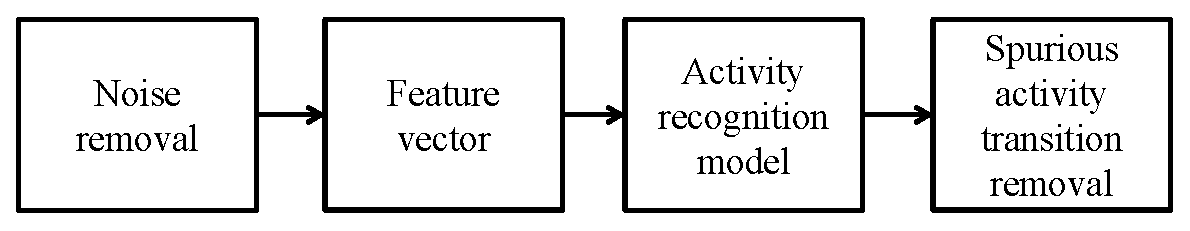
\includegraphics[width=0.9\linewidth]{chap_AR/ARPIPE}
\caption{ARPipe, an activity recognition pipeline.}
\label{fig:ar:pipeline}
\end{figure}

The activity recognition model is constructed with a supervised learning approach, which consists of training and classification steps. In the training step, a set of labeled data is provided to train the model. The second step is used to assign a label to new, unseen data by the trained model. The data in both phases must be pre-processed with the same set of tools, such as filtering and feature vector computation. 

The post-processing phase; that is, spurious activity removal, can also be a model itself and, hence, also requires a learning step. In this case, the pre-processing step also includes activity recognition. Therefore, it is important that the dataset used for training is not the same as that used for the training activity recognition model.


The first two phases in the proposed pipeline are domain-dependent, while the last two phases are general. We demonstrate our methods in the ambient-assisted living domain (see Chapter~\ref{chap:confidence}) to recognize activities performed by an elderly person in a home environment, wearing location-based tags that provide absolute three-dimensional coordinates. The goal is to label an observation vector with eight atomic actions. Specifically, we present two approaches for filtering and feature vector construction to illustrate how they can be used to robustly recognize activities in the presence of noise, clutter, and human action execution variability.



%\section{Motivating Domain}
%\label{sec:ar:problem}


\section{Dealing with Noise}
\label{sec:ar:noise}

\index{noise removal}
An important sensor technology that makes human activity recognition possible relies on real-time location systems (RTLSs). They provide three-dimensional coordinates of tags attached to the human body. High-fidelity optical system, such as \cite{Vicon2009} and SMART \citep{SMART2009}, provide accurate measurements ($\pm 2$ mm), but often include outliers due to marker occlusion and mislabeling. Furthermore, they require a line-of-sight between the body-attached tags and the cameras. They are good for lab use, but fail in real-world applications as they are usually too expensive, hard to install, and have limitations, such as line-of-sight or a confined operational area. More affordable systems rely on radio technology, which is less obtrusive and cheaper, but less accurate. Systems based on ultra-wideband technology (UWB), such as Ubisense~\citep{Ubisense}, achieve $\pm 15$ cm accuracy in an ideal setting, which makes human activity recognition challenging. The main problem addressed in this section is how to de-noise human-motion trajectories captured with UWB RTLS in order to improve activity recognition.

We demonstrate noise filtering on Ubisense, a commercially available localization system. Ubisense allows local positioning by tracking a set of reasonably small tags, which are attached to a person's body. A sampling frequency of around 10 Hz can be achieved with up to four tags attached to a person simultaneously. Each tag maintains radio contact with a stationary sensor (for example, mounted on the wall). These sensors and tags communicate using UWB radio technology. Both the time arrival difference and the radio signal arrival angle are used to calculate the tag position. In a typical open environment, a location accuracy $\pm$15 cm can be achieved across 95\% of the readings. However, in real-life scenarios the accuracy occasionally exceeds $\pm$ 200 cm, which represents quite a challenge for preprocessing and filtering. 

%Generally, more tags worn by a person enables more accurate activity recognition; however, given large enough noise, even an increased number of tags does not necessarily improve the results. For example, it turns out that the accuracy of the activity-recognition model was comparable when using only eight or four tags [ref]. However, having less than two tags significantly impacts the activity recognition accuracy. Since more tags require more effort from the person, it is desirable to use as little tags as possible. It this section we show an approach using four tags attached to at the following locations on the body (as shown in Figure~\ref{fig:tags}): chest, waist (optional), left and right ankles.

De-noising human motion captured with UWB sensors raises several challenges. First, motion-capture data may contain a certain percentage of missing values due to packet loss, temporal sensor disability, low battery, etc. Second, due to sensor noise and environment disturbances, motion-capture data often include outliers and unstable measurements, which corrupt body posture reconstruction. This results in a violation of physical body constraints as well as spatio-temporal body constraints, which in turn introduces additional noise into the activity recognition models. Finally, essential activity recognition features that are computed from noisy measurements (for example, velocity, acceleration) may have an integral error term; that is, the error accumulates over time.

In this section, we propose an efficient approach for de-noising human-motion trajectories that not only filters corrupted motion data, but also enforces the human body's spatio-temporal constraints and enables more accurate feature computation. The key idea is to construct a series of filters that addresses the above-mentioned challenges.

% :\\
% (i) median\\
% (ii) body\\
% (iii) Kalman\\
% (iv) adaptive low-pass  

%
%	? vrstni red filtrov
%	? body filter kot kalmanov filter
%	mediana (B)
%	body filter (B)
%	kalmanov filter (izracuna tudi hitrosti, ki jih ne merimo direktno = feature za ML) (B prpi?i)
%	is moving (R predelaj)
%	low pass filter (R+B)
%	setting parametters:
%		mediana: dolzina okna
%		body: izmeri cloveka
%		kalman: std odkloni iz analize suma
%		is moving: iz analize suma
%		low-pass: parameter za nastavljanje lambde


% In this section we introduce a set of filters that address...

\subsection{Dealing with Outliers}
\label{sec:ar:noise:median}

% Idea: weighted median filter \cite{Yin1996median}

Median filter is a non-linear filter that can suppress impulsive, isolated noise without blurring sharp changes in the signal \citep{Yin1996median}. The filter consists of a sequential sample window with odd length $w=2n+1$. At each time step $t$, the filter returns the median of the elements in the window:
\begin{equation}
	x_t' = \text{median}(x_{t-n}, ..., x_t, ..., x_{t+n}).
\end{equation}

The only parameter of the median filter is the window length $w$, which introduces a delay of length $\lfloor w/2 \rfloor$. A larger window size may smooth the signal too much, while a smaller window size may not remove the high density noise. A common approach is to choose a window length such that desired signal features are preserved while attenuating noise.

%The majority of computational time is spent on calculating the media of each window, hence an efficient median calculation is crucial for the filter speed. While a vanilla approach sorts samples in every window, histogram-based algorithms implemented with binary trees can be more efficient [?].

In our case, we apply the median filter at each tag, separately for each dimension. The filter removes isolated spikes in the signal, while parts with high oscillation remain unsuppressed.



\subsection{Missing Values and Velocity Estimation}
\label{sec:ar:noise:kamlan}

Motion capture data contains missing values due to packet loss or delay during transmission, sensor failure, corrupted packets, etc. Our first goal is, hence, to fill the missing values. Furthermore, we would like to estimate additional quantities such as velocity. For this task, we use the recursive linear Kalman filter \citep{Kalman1960} for optimally estimating he system's state, assuming that the underlying system is a linear dynamical system and that all measurement errors have a multivariate Gaussian distribution. The underlying system, that is, human body, is assumed to be reasonably approximated by a linear dynamical system. Even though the original measurement error distribution is not Gaussian, the median filtering removes signal spikes, which results in a measurement error distribution that better resembles Gaussian distribution.

The Kalman filter performs the following three tasks: smoothing of the UWB measurements, estimating the velocities of tags, and predicting the missing measurements. We defined filter state as a six-dimensional observation vector $\mathbf{x}_t$ that includes positions and velocities in each of the three dimensions at time $t$, $\mathbf{x}_t=[p_{x, t}, p_{y, t}, p_{z, t}, v_{x, t}, v_{y, t}, v_{z, t}]^\intercal$.

The next state is estimated from the previous state as follows:
\begin{equation}
\label{eq:kalmanUpdate}
\mathbf{x}_{t+1} = \mathbf{F} \mathbf{x}_t + \mathbf{B} \mathbf{u}_t + \mathbf{w}_t,
\end{equation}
where $\mathbf{F}$ encodes the linear dynamical system, $\mathbf{B}$ is a control matrix and $\mathbf{w}_t$ is noise covariance matrix. In our case, the Kalman update is  simplified to Equation~(\ref{eq:kalman}). The next state is calculated as a sum of the previous position and a product of the previous velocity and the time between the consecutive measurements $\Delta t$ for each direction separately. The velocities remain constant. The measurement noise covariance matrix was set based on UWB system specification, while the process noise covariance matrix was fine-tuned experimentally. 
\begin{equation}
\label{eq:kalman}
\begin{bmatrix}
p_{x, t+1} \\
p_{y, t+1} \\
p_{z, t+1} \\
v_{x, t+1} \\
v_{y, t+1} \\
v_{z, t+1}
\end{bmatrix} 
=
\begin{bmatrix}
1 & 0 & 0 & \Delta_t & 0 & 0 \\
0 & 1 & 0 & 0 & \Delta_t & 0 \\
0 & 0 & 1 & 0 & 0 & \Delta_t \\
0 & 0 & 0 & 1 & 0 & 0 \\
0 & 0 & 0 & 0 & 1 & 0 \\
0 & 0 & 0 & 0 & 0 & 1 \\
\end{bmatrix} 
\begin{bmatrix}
p_{x, t} \\
p_{y, t} \\
p_{z, t} \\
v_{x, t} \\
v_{y, t} \\
v_{z, t}
\end{bmatrix}
+ \mathbf{w}_t.
\end{equation}

%\subsection{Adaptive Low-Pass Filter}
%\label{sec:ar:noise:isMoving}

%\subsubsection{Movement Detection}

%\subsubsection{Low-Pass Filtering}



\subsection{Spatio-Temporal Body Constraints}
\label{sec:ar:noise:body}
Up to this point, each tag was considered as a separate measurement. In reality, the tags are attached to a human body, which implies a set of tag position constraints. In activity recognition, it is expected that a set of measurements resembles human body proportions as well as spatio-temporal patterns in natural human motion. We construct a filter based on iterative constraint relaxation that: (i) projects measured values in a valid domain; (ii) applies human body constraints to the measured positions; and (iii) constrains spatio-temporal motion patterns.

%\subsubsection{Mapping Measurements to a Valid Domain}
In the first step, we make an assumption about valid measurement domain. For example, we expect all the measurements to be within a room, that is, cuboid, bounded with two extreme points $\mathbf{p}_X$ and $\mathbf{p}_Y$ (assuming the coordinate system is aligned with the room). 
%To keep a new measurement $\mathbf{p}_t$ within the expected bounds, it has to be translated to an edge (in case it is not already within the cuboid) as shown in Figure~\ref{fig:cuboid}:
%\begin{equation}
%\label{eq:validDomain}
%p_A \leq p_t \leq  p_B.
%\end{equation} 
To keep the measurement $\mathbf{p}_t$ within the expected bounds, it has to be translated to an edge (in case it is not already within the cuboid) as shown in Figure~\ref{fig:cuboid}. The update step is:
\begin{equation}
\label{eq:validDomain}
\mathbf{p}_t' = \min(\max(\mathbf{p}_t, \mathbf{p}_X), \mathbf{p}_Y).
\end{equation} 

\begin{figure}[!h]
\centering
\includegraphics[width=0.4\textwidth]{img/box}
\caption{All the measurements are bounded within a cuboid.}
\label{fig:cuboid}
\end{figure}


%\subsubsection{Body Constraints}
We model the human body using rigid-body components, which assume that there is no deformation.   Rigid-body components are connected to each other with joints and form an \textit{articulated rigid body} that approximates the human body as shown in Figure~\ref{fig:tags:noise}. The distance between any two connected joints is constant regardless of external forces. Note that at this point we do not pose any joint constraints.

\begin{figure}[!h]
\centering
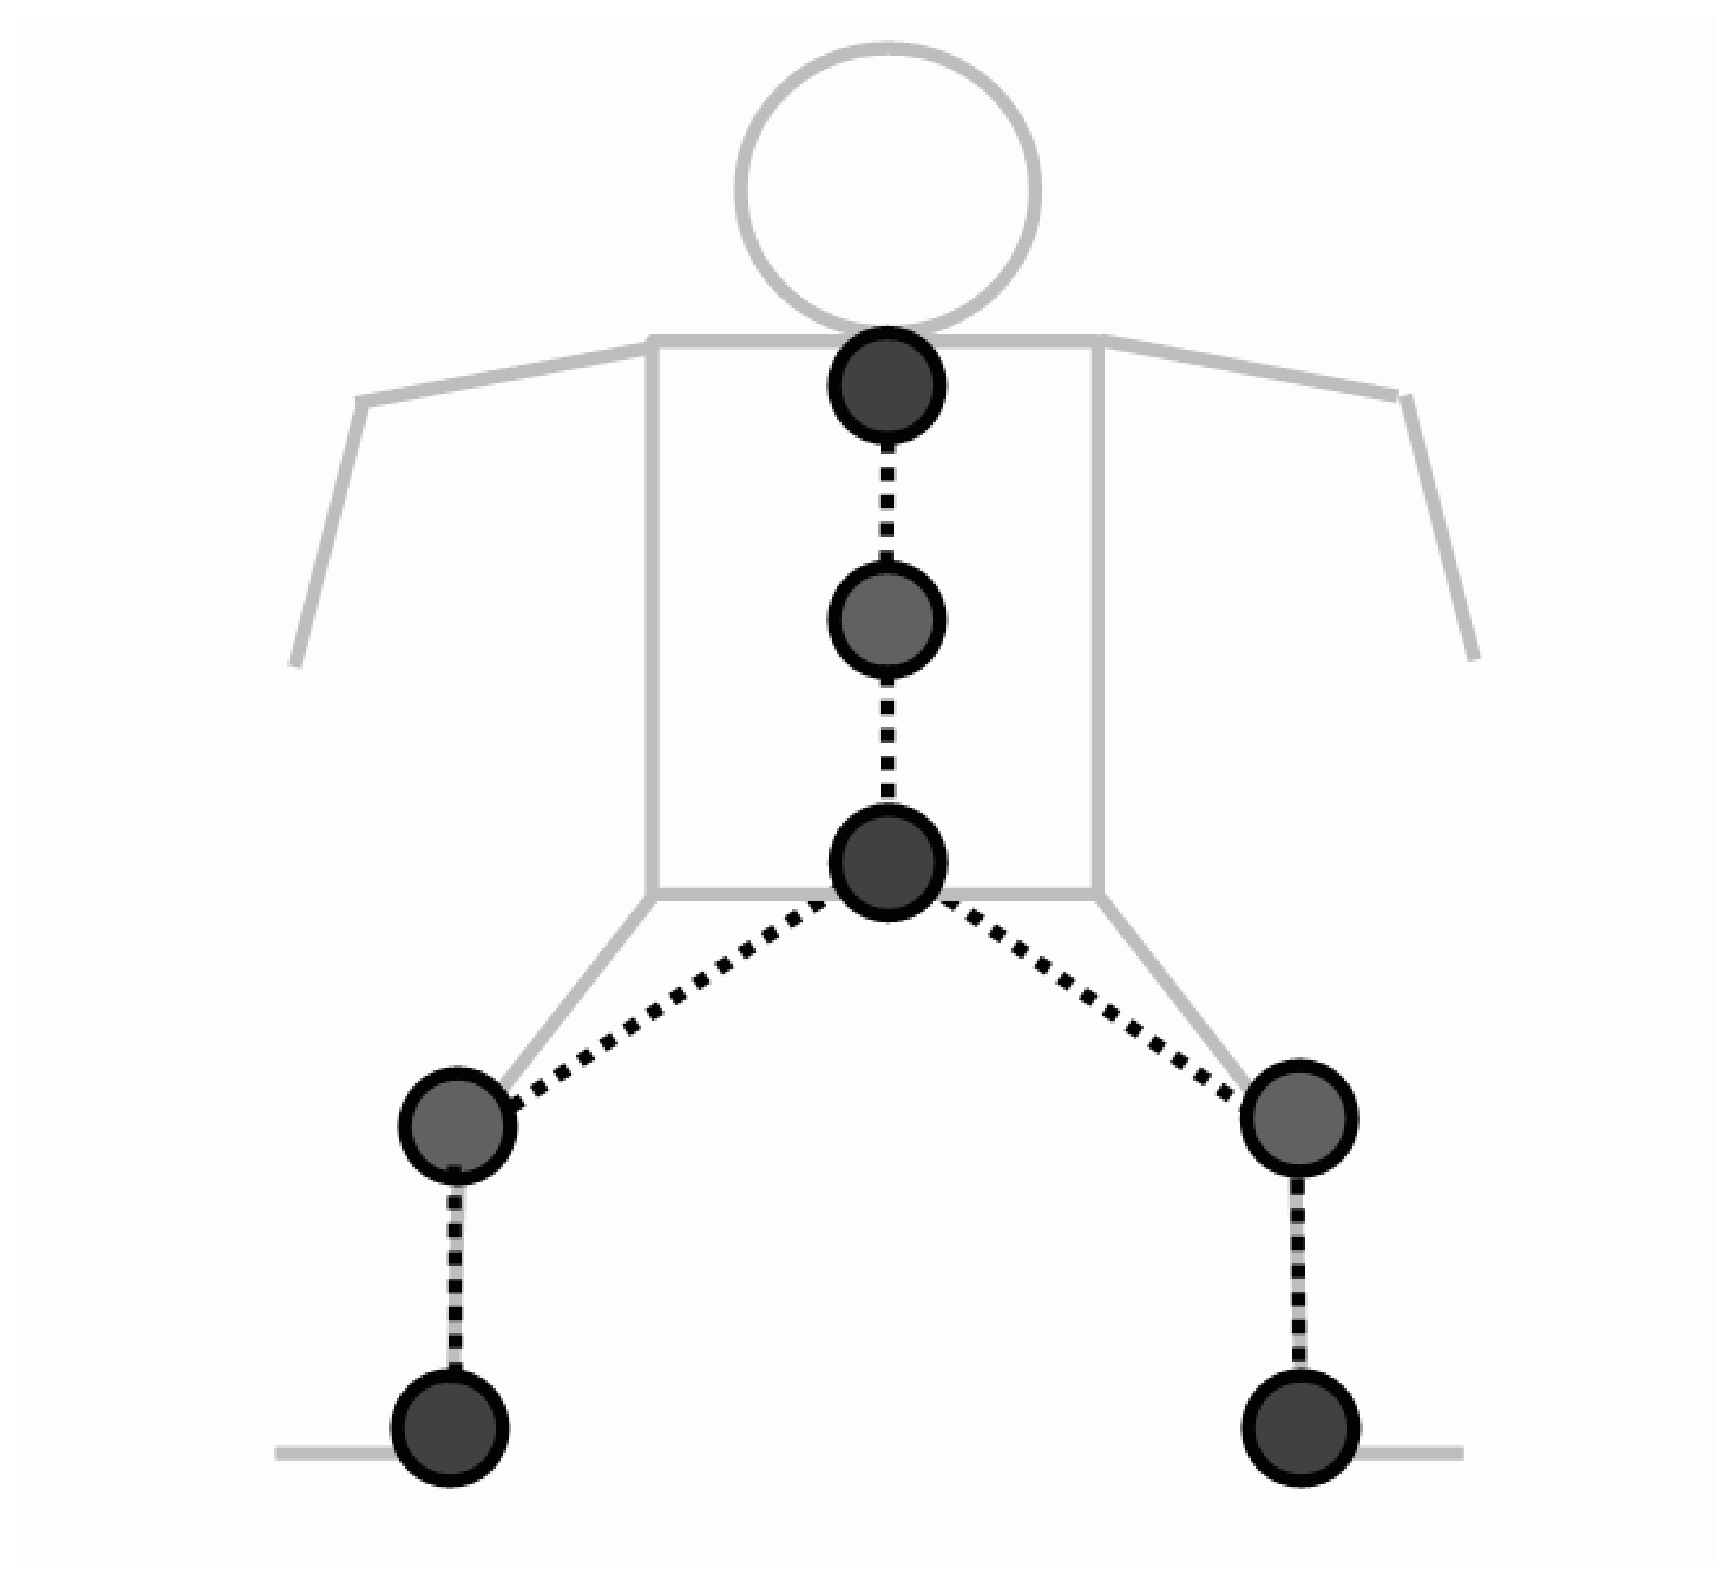
\includegraphics[width=5cm]{img/tags1}
%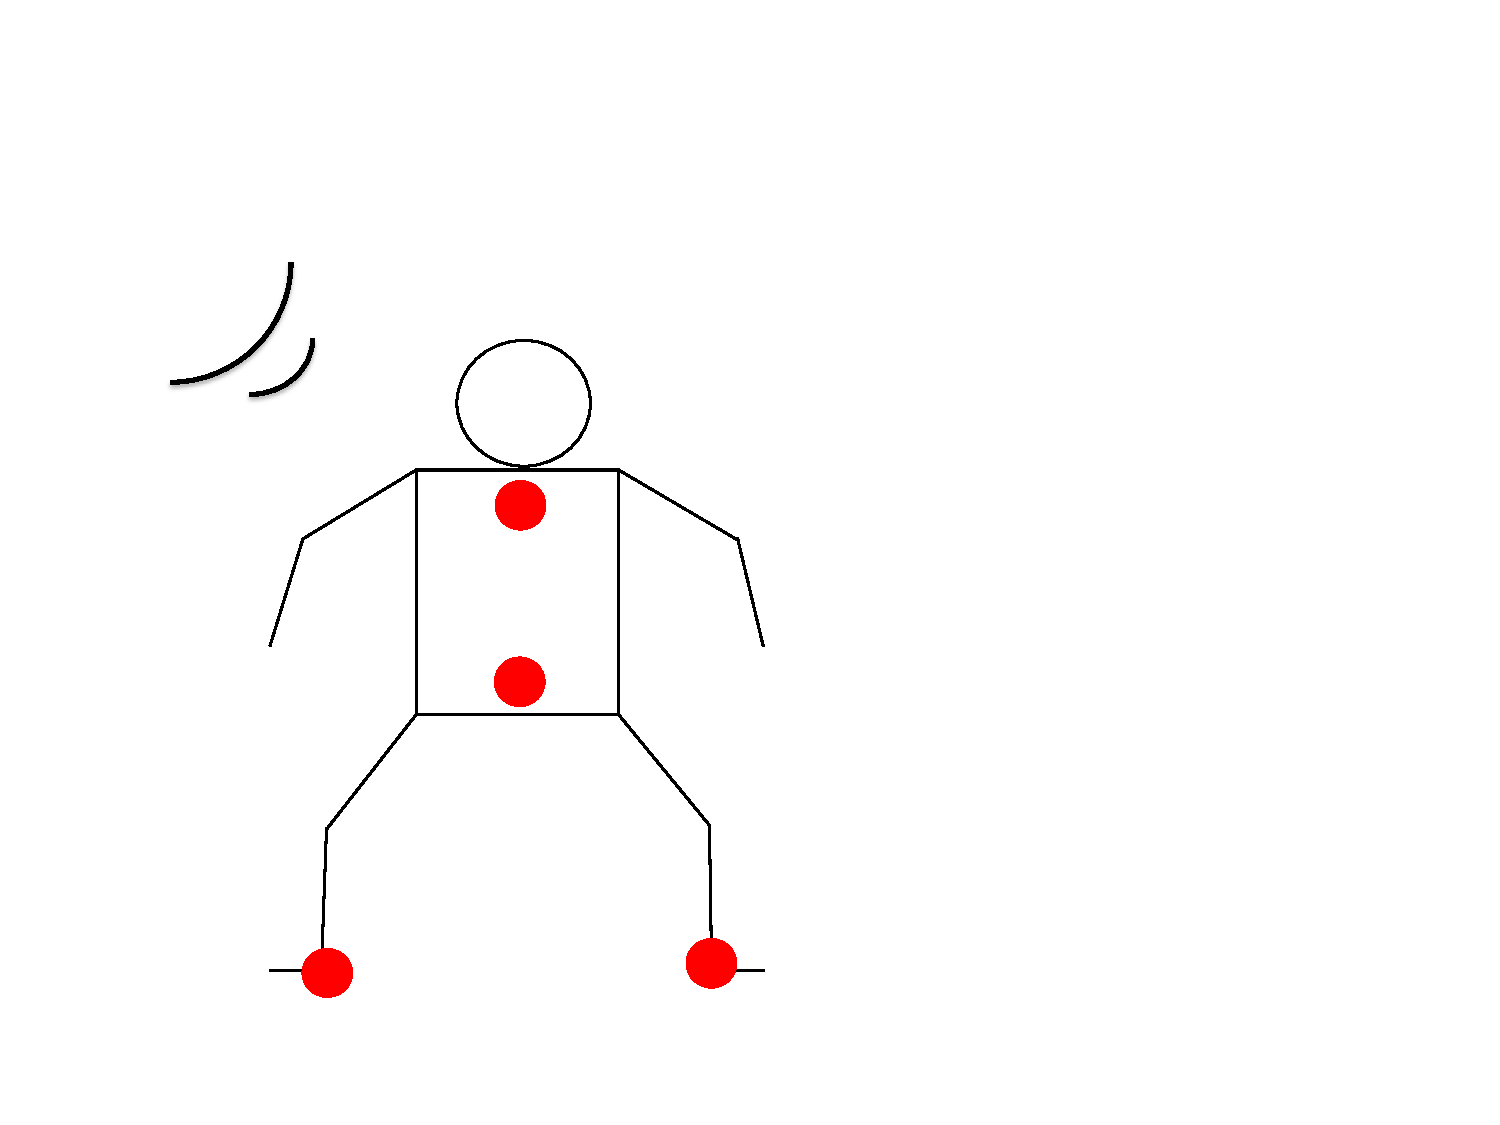
\includegraphics[bb=220 300 340 410, width=5cm]{img/tags.pdf}
\caption{Human body is modeled with an articulated rigid body.}
\label{fig:tags:noise}
\end{figure}

In our case, the four RTLS tags provide the joint positions (ankles, waist, and chest), but do not allow reconstructing the skeleton displayed in Figure~\ref{fig:tags:noise} since the knees and abdomen are missing. 

The missing joints are reconstructed as follows: suppose we have two points $A$ and $C$ with known positions and a joint $B$ that interconnects $A$ and $C$, with an unknown position. Since the distances $r_A=d(A, B)$ (between $A$ and $B$) and $r_c=d(C, B)$ are known, the point $B$ then lies at the intersection of two spheres, centered at $A$ with radius $r_A$ and at $C$ with radius $r_C$. 

In general, there are three cases when the measurements are obtained: (i) $r_A+r_B=d$, that is, the intersection includes a single point; (ii) $r_A+r_B>d$, that is, there is no solution; and (iii) $r_A+r_B<d$, that is, the intersection consists of a circle. In the second case we position the point $B$ on a line between points $A$ and $C$ so that the distances between points is in the same proportion as the lengths of $r_A$ and $r_B$.
%
In the third case, we proceed as follows: to calculate the position of the point $B$, we use a new coordinate system in which the first sphere is centered at the origin and the second sphere is centered at a point on the positive x-axis, at distance $d$ from the origin, as shown in Figure~\ref{fig:sphere-sphere}. Subtracting the sphere equations, we find a set of points representing a circular intersection of the spheres:
\begin{eqnarray}
\label{eq:circle}
x = \frac{d^2 - {r_C}^2 + {r_A}^2}{2d}, \\
\label{eq:circle1}
y^2 + z^2 = {r_A}^2 - (\frac{d^2 - {r_C}^2 + {r_A}^2}{2d})^2.
\end{eqnarray}
We are not interested in the exact position of B, hence we pick an arbitrary point from the circle and transform it to the original coordinate system.  As explained below, the distance between joints is enforced with Equations~(\ref{eq:fixDistance}) and (\ref{eq:fixDistance1}).

\begin{figure}[!h]
\centering
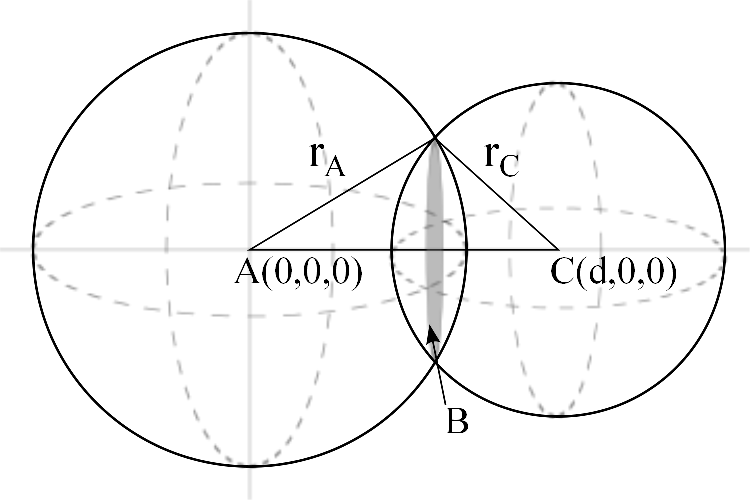
\includegraphics[width=0.5\textwidth]{img/sphere-sphere}
\caption{The result of sphere-sphere intersection is a circle.}
\label{fig:sphere-sphere}
\end{figure}

Once we have all the joint positions we can introduce constraints between the connected pairs. For example, suppose the true distance between joints A and  B is $r_A$, that is,
\begin{equation}
\label{eq:constraint}
\|\mathbf{p}_A - \mathbf{p}_B\| = r_A.
\end{equation}
If measurements $p_{A}$ and $p_B$ violate the constraint given by Equation~(\ref{eq:constraint}), the position of both points is adjusted \citep{Jakobsen2001}. 
%We differentiate two cases. In the first case, the measured distance is less than the true distance; that is, $d(p_A, p_B) < r_A$.
Each point is translated along the line connecting the points for half of the error defined as the difference between the measured and the true distance as shown in Figure~\ref{fig:distance-fix}. The update is:
\begin{eqnarray}
\label{eq:fixDistance}
\mathbf{p}'_A = \mathbf{p}_A + \frac{\|\mathbf{p}_B-\mathbf{p}_A\| - r_A}{2\|\mathbf {p}_B-\mathbf{p}_A\|}(\mathbf{p}_B-\mathbf{p}_A),\\
\label{eq:fixDistance1}
\mathbf{p}'_B = \mathbf{p}_B - \frac{\|\mathbf {p}_B-\mathbf{p}_A\| - r_A}{2\|\mathbf{p}_B-\mathbf{p}_A\|}(\mathbf {p}_B-\mathbf{p}_A).
\end{eqnarray}

\begin{figure}[!h]
\centering
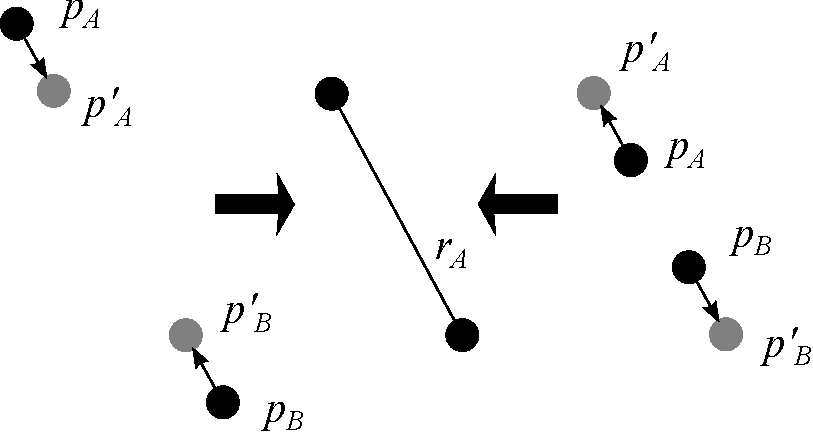
\includegraphics[width=0.5\textwidth]{img/distance-fix}
\caption{Move the points $\mathbf{p}_A$ and $\mathbf{p}_B$ to match the constraint given by Equation~(\ref{eq:constraint}).}
\label{fig:distance-fix}
\end{figure}

%Articulated rigid bodies & joint constraints


%\subsubsection{Spatio-Temporal Motion Patterns}
In addition to the constraints introduced by human body proportions, we also consider physical motion constraints such as velocity and acceleration, of limbs. Suppose that  $a$~m/s$^2$ is the greatest possible acceleration of an ankle. This implies that it can travel at most $l=(v_{t-1}+a\Delta t/2)\Delta t$ meters in time interval $\Delta t$, where $1/\Delta t$ is the sampling frequency. Hence, the next ankle's position $\mathbf{p}_{t}$ is limited with a sphere with radius $l$, that is, 
\begin{equation}
\|\mathbf{p}_{t} - \mathbf{p}_{t-1}\| \leq l.
\end{equation}
In case the new position is outside the sphere, the position is translated on the edge of the sphere in the direction of the measurement. The update step is:
\begin{equation}
\mathbf{p}'_t = \mathbf{p}_t + \frac{l (\mathbf{p}_t - \mathbf{p}_{t-1})}{\|\mathbf{p}_t-\mathbf{p}_{t-1}\|}.
\end{equation}


%image with sphere
%In order to speed up the computations we  approximate the sphere with a cube with edge length $l$. In this case we can limit the new position using Equation~\ref{eq:validDomain}. 


%\subsubsection{Iterative Constraint Relaxation}

Finally, all the constraints are put together. Consider $\mathbf{C}=\{\Phi_i\}$ as a set of constraints, where $\Phi(\mathbf{p})$ applies the update step on point $\mathbf{p}$ using Equation~(\ref{eq:validDomain}); that is, $\mathbf{p}' \leftarrow \Phi(\mathbf{p})$, while $\Phi(\mathbf{p}_A, \mathbf{p}_B)$ applies the update step on both points $A$ and $B$ using Equations~(\ref{eq:fixDistance}) and (\ref{eq:fixDistance1}); that is, $\mathbf{p}'_A, \mathbf{p}'_B \leftarrow \Phi(\mathbf{p}_A, \mathbf{p}_B)$.  If a constrained between points $A$ and $B$ is not present, then $\Phi(\mathbf{p}_A, \mathbf{p}_B)$ does not alter the corresponding points.
The algorithm below takes the set of constraints and its value updates as an input and iteratively updates the values until the convergence threshold $\tau_c$ or maximal number of iterations $k$ is reached.

\begin{algorithm}
\caption{Iterative constraint relaxation.}
\label{alg:LOF}
\begin{algorithmic}
\REQUIRE set of constraints $\mathbf{C}$, set of points $\mathbf{P}$, maximal number of iterations $k$, convergence threshold $\tau_c$
\ENSURE set of points $P$
\REPEAT
	\STATE $\Delta = 0$
	\FOR{$\mathbf{p} \in \mathbf{P}$}
		\FOR{$\mathbf{q} \in \mathbf{P}$}
			\STATE $\mathbf{p}', \mathbf{q}' \leftarrow \Phi(\mathbf{p}, \mathbf{q})$
			\STATE $\Delta \leftarrow \Delta + |\mathbf{q}-\mathbf{q}'|$
			\STATE $\mathbf{q} \leftarrow \mathbf{q}'$
		\ENDFOR
		\STATE $\mathbf{p}' \leftarrow \Phi(\mathbf{p})$
		\STATE $\Delta \leftarrow \Delta + |\mathbf{p}-\mathbf{p}'|$
		\STATE $\mathbf{p} \leftarrow \mathbf{p}'$
	\ENDFOR
	\STATE $k \gets k-1$
\UNTIL{$k > 0$ \AND $\Delta > \tau_c$}
\end{algorithmic}
\end{algorithm}


An example of filter effects is shown in Figure~\ref{fig:noise}, which shows $x$ (top), $y$ (middle) and $z$ (bottom) coordinates for a tag attached to the waist for $T=600$ time steps (one time step lasts approximately $1/8$ s). The vertical axis corresponds to meters. The blue line represents the original location measurements, the green line represents the median filter result, and the red line represents the Kalman filtering and spatial body constraints results.
\begin{figure}[!h]
\centering
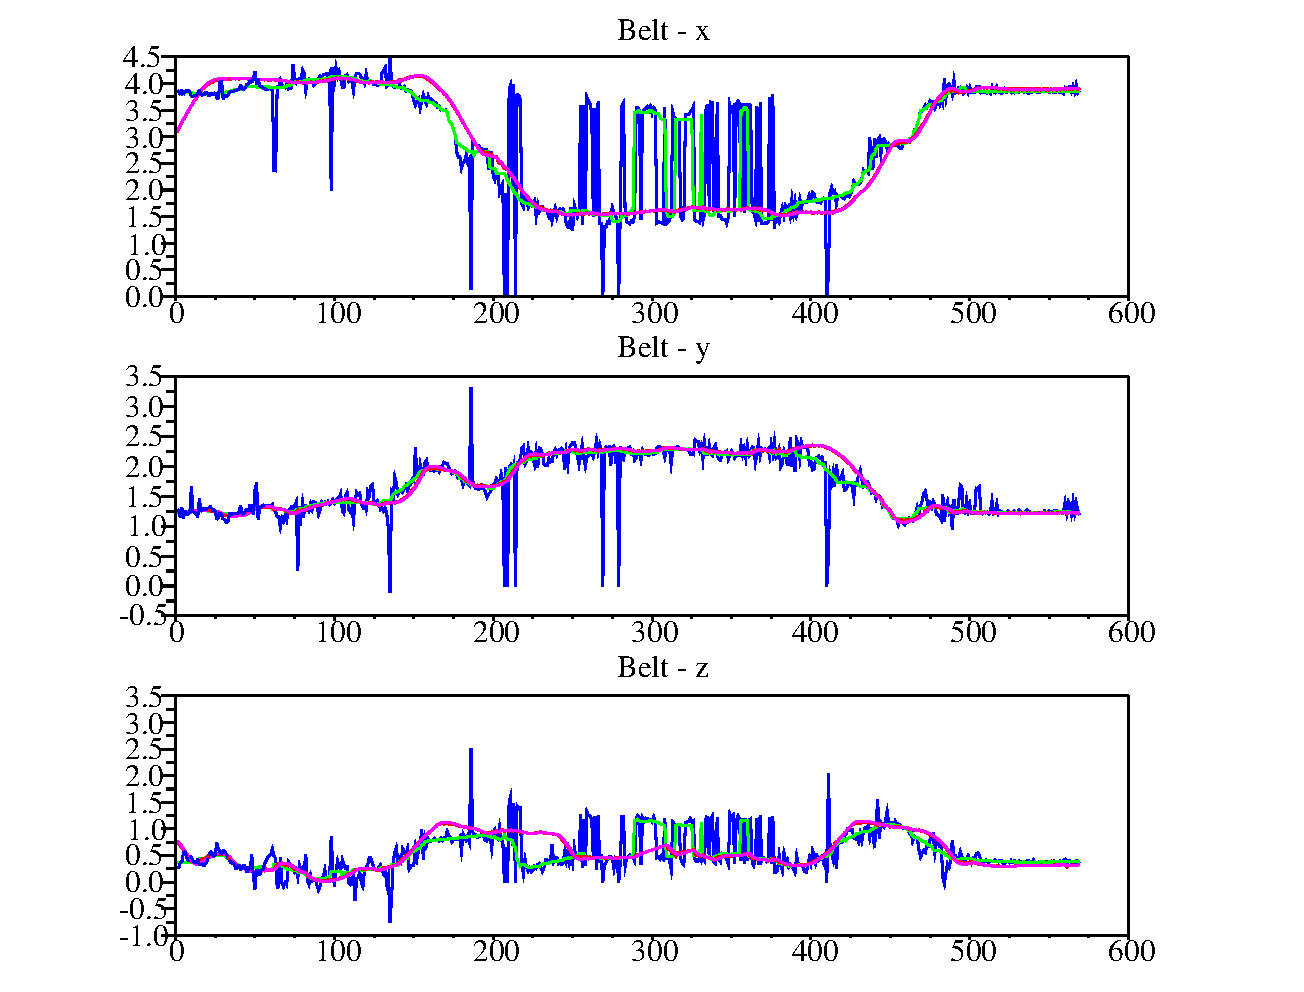
\includegraphics[width=0.85\linewidth]{chap_AR/cld-belt}
\caption{Filtered coordinates $x$ (top), $y$ (middle) and $z$ (bottom) of a tag attached to the waist.}
\label{fig:noise}
\end{figure}


%
%==========================================================================================
%
\section{Feature Vector}
\label{sec:ar:ml}

%The goal is to assign an activity $a$ from a set of possible actions in  $\mathbb{A}$ to an observation $x_t$. This section first discusses a 

%The goal of our research was to classify the person’s behavior into one of the following activities: falling, lying down, sitting down, standing/walking, sitting and lying. To obtain training data for a classifier to recognize these activities, we recorded 45 examples of the behavior of three persons. Each recording consisted of multiple activities:
%•	3 × 15 recordings of falling, consisting of standing/walking, falling and lying.
%•	3 × 10 recordings of lying down, consisting of standing/walking, lying down and lying.
%•	3 × 10 recordings of sitting down, consisting of walking, sitting down and sitting.
%•	3 × 10 recordings of walking.
%The recordings consisted of the coordinates of 12 body tags attached to the shoulders, elbows, wrists, hips, knees and ankles. This is the full complement of tags that will probably be reduced in the future. Since the equipment with which the Confidence system will acquire tag coordinates is still under development, the commercially available Smart infrared motion capture system [6] was used instead. The coordinates were acquired with 60 Hz. The frequency was afterwards reduced to 10 Hz, which is the expected Confidence data acquisition frequency. To make the recordings even more similar to what we expect of the Confidence equipment, we added Gaussian noise to them. The standard deviation of the noise was 4.36 cm horizontally and 5.44 cm vertically. This corresponds to the noise measured in the Ubisense real time location system [19]. The Ubisense system is similar to the equipment planned for acquiring tag coordinates in Confidence. The noise in the recordings was smoothed with Kalman filter [14].



%\subsection{Features}

Finding an appropriate representation of the person's activities is probably the most challenging part of activity recognition. The behavior needs to be represented with simple and general features, so that the model using these features will also be general and work well on behaviors different from those in the learning set. 
In fact, it is not difficult to design features specific to captured observations in a training set; such features would work well on them. However, since the training set captures only a part of the whole range of human behavior, overly specific features would likely fail on general behavior.

\begin{definition}
\label{def:feature}
	\emph{Feature vector} $\mathbf{f}_t$ at time step $t$ is a vector of descriptors obtained from observation $\mathbf{x}_t$. 
\end{definition}
\noindent
Feature $\mathbf{f}_t$ can hence contain values from observation as well as additional values computed from observation $\mathbf{f}_t$ or other observations. In general, the feature vector can be interpreted as observation extended with additional descriptors that capture targeted behavior.

\subsection{Features}

\index{feature extraction}
We propose three sets of features describing the person behavior in a selected domain. We demonstrate a possible feature set on a kinematic model of a human with 12 points as shown in Figure~\ref{fig:kinematic} to illustrate potential variety. In practice, however, it is possible to use a reduced feature set. First, reference features are expressed in the reference coordinate system, which is fixed with respect to the person's environment. Second, body features are expressed in a coordinate system affixed to the person's body. Third, angle features are the angles between adjacent body parts.

\begin{figure}[!h]
\centering
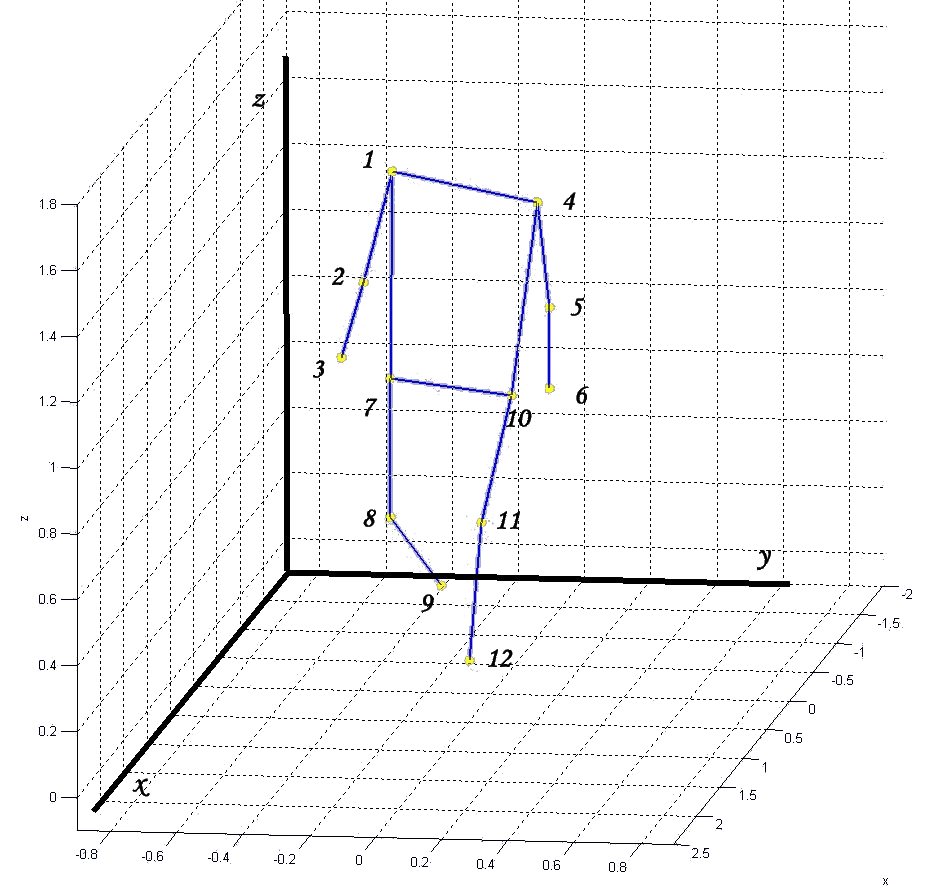
\includegraphics[width=0.7\linewidth]{chap_AR/kinematic_model}
\caption{Kinematic model of a human body.}
\label{fig:kinematic}
\end{figure}

\subsubsection{Reference Features}
When selecting reference features, the $x$ and $y$ coordinates are usually ignored, since these coordinates describe the person's location in the environment, but the activities of interest can generally take place at any location. A reasonable set of features can include $z^{(i)}_t$ coordinate of sensor tag $i$ at time $t$, the velocity of sensor tag in $z$ direction $v^{(i)}_t$, the absolute distance $d^{(i,j)}_t$between sensor tags $i$ and $j$, and others.


\subsubsection{Body Features}
Body features are expressed in a coordinate system affixed to the person's body. This makes it possible to observe $x$ and $y$ coordinates of the person's body parts, since these coordinates no longer depend on locations within the environment.

The body coordinate system is shown in Figure~\ref{fig:body_coordinate}. Its origin $\mathbf{o}$ is at the mid-point of the line connecting the hip tags ($\mathbf{p}_7$ and $\mathbf{p}_{10}$ in Figure~\ref{fig:body_coordinate}). This line also defines the $y$ axis, which points towards the left hip. The $z$ axis is perpendicular to the $y$ axis, touches the line connecting both shoulder tags ($\mathbf{p}_1$ and $\mathbf{p}_4$ in Figure~\ref{fig:body_coordinate}) at point $\mathbf{p}_z$, and points upwards. The $x$ axis is perpendicular to the $y$ and $z$ axes and points forwards.


\begin{figure}[!h]
\centering
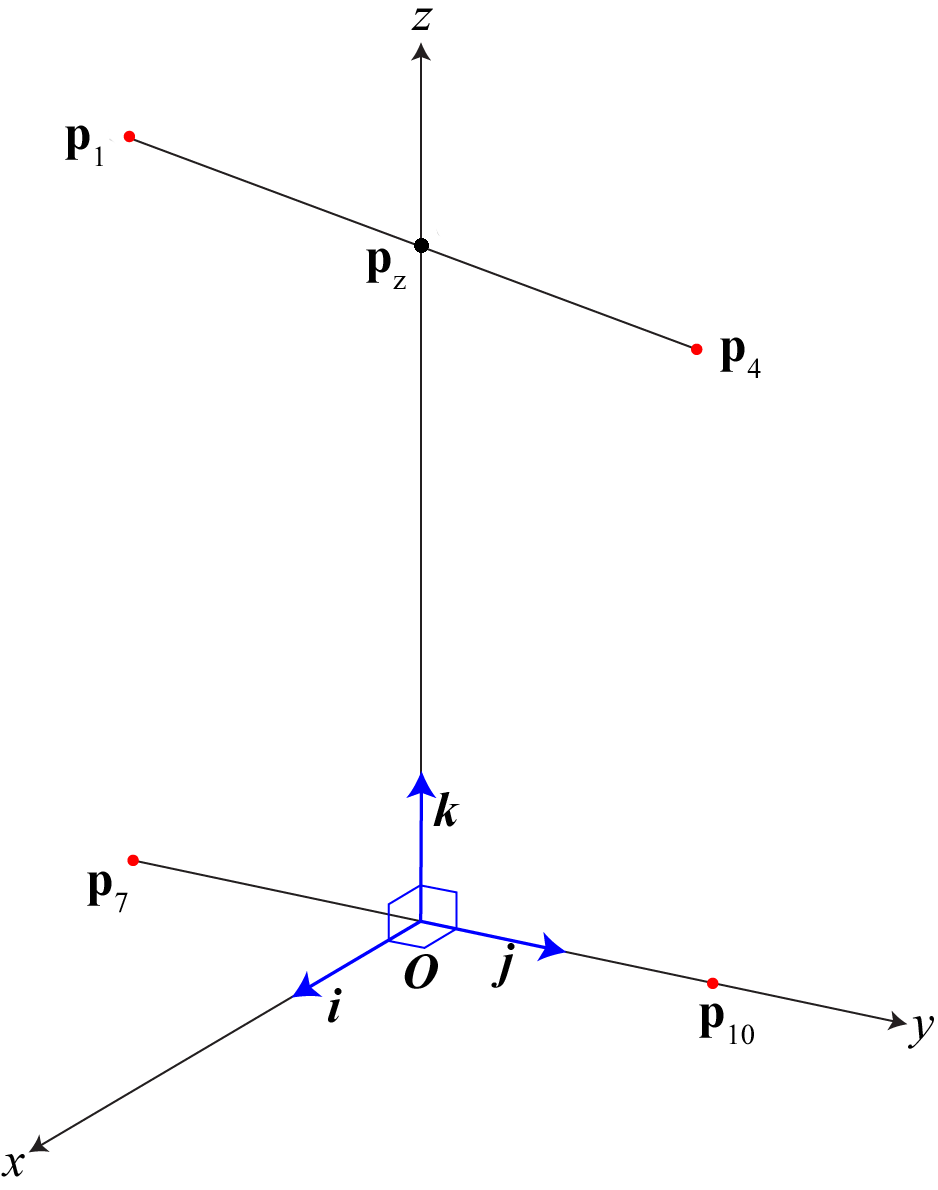
\includegraphics[width=0.5\linewidth]{chap_AR/body_coordinates}
\caption{The body coordinate system.}
\label{fig:body_coordinate}
\end{figure}

In order to translate reference coordinates into body coordinates, Equation~(\ref{eq:origin}) expresses the origin $\mathbf{o}$ and basis $(\mathbf{i}, \mathbf{j}, \mathbf{k})$ of the body coordinate system in the reference coordinate system, which gives us the basis vector $\mathbf{j}$:

\begin{equation}
\label{eq:origin}
\mathbf{o}=\frac{\mathbf{p}_7 + \mathbf{p}_{10} }{2},
\end{equation}

\begin{equation}
\label{eq:basis_j}
\mathbf{j}=\frac{\mathbf{p}_7 - \mathbf{o} }{|\mathbf{p}_{10} - \mathbf{o}|}.
\end{equation}

\noindent
To obtain the basis vector $\mathbf{k}$, Equation~(\ref{eq:p_z}) is first used to calculate $\mathbf{p}_z$; Equation~(\ref{eq:basis_k}) then gives us $\mathbf{k}$:
\begin{equation}
\label{eq:p_z}
\mathbf{p}_z = \mathbf{p}_7 + a(\mathbf{p}_4 - \mathbf{p}_7),
\end{equation}

\begin{equation}
a 	= \frac{(\mathbf{p}_1 - \mathbf{o}) \cdot (\mathbf{p}_{10} - \mathbf{p}_7)}{(\mathbf{p}_4 - \mathbf{p}_1) \cdot  (\mathbf{p}_{10} - \mathbf{p}_7)},
\end{equation}

\begin{equation}
\label{eq:basis_k}
\mathbf{k}=\frac{\mathbf{p}_7 - \mathbf{o} }{|\mathbf{p}_{10} - \mathbf{o}|}.
\end{equation}

Finally, we obtain basis vector $\mathbf{i}$ using Equation~(\ref{eq:basis_i}):
\begin{equation}
\label{eq:basis_i}
	\mathbf{i}=\mathbf{j} \times \mathbf{k}.
\end{equation} 

	 
To translate a point $\mathbf{p}$ coordinates in the reference coordinate system into the body coordinate systems, Equation~(\ref{eq:transform}) is used. The vector $\mathbf{p}_R = (x_R, y_R, z_R, 1)$ corresponds to the point $\mathbf{p} = (x, y, z)$ in the reference coordinate system. The vector $\mathbf{p}_B = (x_B, y_B, z_B, 1)$ corresponds to the point $\mathbf{p}=(x_B, y_B, z_B)$ in the body coordinate system. Matrix $\mathbf{T}_{R \rightarrow B}$ is the transformation matrix from the reference to the body coordinate system. 

\begin{equation}
\label{eq:transform}
\mathbf{p}_B=\mathbf{T}_{R \rightarrow B} \mathbf{p}_B^\intercal,
\end{equation} 
$$
 \mathbf{T}_{R \rightarrow B} = \begin{bmatrix}
        \mathbf{i}_x &	\mathbf{i}_x &	\mathbf{i}_x &	-\mathbf{o} \cdot \mathbf{i} \\
        \mathbf{j}_x &	\mathbf{j}_x &	\mathbf{j}_x &	-\mathbf{o} \cdot \mathbf{i} \\
        \mathbf{k}_x &	\mathbf{k}_x &	\mathbf{k}_x &	-\mathbf{o} \cdot \mathbf{i} \\
        0 &	 			0 &				0 &				1
      \end{bmatrix}.
$$

Based on the above equations, a reasonable set of body attributes may include the tag's body features, absolute velocity, and the angles of movement with respect to the $z$ axis and $xz$ plane, and others.

\subsubsection{Angle Features}	

Once the body coordinate system is obtained, it is possible to compute an advanced set of features describing relative angles between different body parts represented by quaternions. Unit quaternions provide a convenient mathematical notation for representing object orientations and rotations in three dimensions. Compared to Euler angles, they are simpler and avoid the gimbal lock problem. Compared to the rotation matrices, they are more efficient and numerically stable. %Quaternions have found their way into applications in computer graphics, robotics, navigation, and orbital mechanics of satellites. 

This thesis will not go into further details on angle equations; the reader is referred to \cite{Lustrek2008report} for details. A reasonable set of attributes may include the angles of the left and right elbow, the left and right knee, the left and right shoulder (represented by quaternions), the left and right hip (also represented by quaternions), and others.


\subsection{Canonical Representation}
\index{canonical representation}
Due to its continuous nature, determining the exact transition points between activities is difficult. We address this issue by combining features into short, overlapping time windows during which we assume that a single activity is dominant. We denote this representation as canonical form that represents the equivalence classes. To test whether two activities in specific time interval are equivalent, it suffices to test their canonical forms for equality. A canonical form thus enables classification and gives a distinguished (canonical) representative of an action.

In practical terms, one wants to be able to recognize the canonical forms; that is, overlapping windows. Each window is classified independently as described in the next section (Section~\ref{sec:ArModel}).

More formally, we define:
\begin{itemize}
	\item $w$ is window length that contains an even number of observations,
	\item $i$ is an index over $|w|$ elements in window, and
	\item $j$ is an index over $W$ overlapping windows.
\end{itemize}

Given a sequence of observations $\{\mathbf{x}_1, \mathbf{x}_2, ..., \mathbf{x}_T\}$, we first compute the sequence of features $\{\mathbf{f}_1, \mathbf{f}_2, ..., \mathbf{f}_T\}$. Then, for constants $m$ and $n$, where $m$ is the number of elements before $t$, and $n$ after $t$; that is, $m+n=|w|+1$, we construct $W_j$, $1 \leq j \leq (|T|-|w|+1)$ windows such that
\begin{equation}
\label{eq:window}
W_j = \{\mathbf{f}_i | j - m \leq i \leq j + n \}.
\end{equation}
Each $W_j$ is labeled with a dominant activity from $\mathbb{A}$ that is assigned to the feature vector $\mathbf{f}_t$. Note, that Equation~(\ref{eq:window}) allows $\mathbf{f}_t$ to adopt any position in $W_j$; in practice it is placed at the beginning ($m=0$), middle ($m=n$), or at the end ($n=0$).
%
An example for $w=9$ and $m=n=4$ is shown in Figure~\ref{fig:canonical}. First, each feature vector is constructed by three sets of attributes. Then, the vector is presented in canonical representation with a window. The end of the window is labeled with the dominant activity.
%observation are captured for 10 time steps and extended to feature vectors. ...

\begin{figure}[!h]
\centering
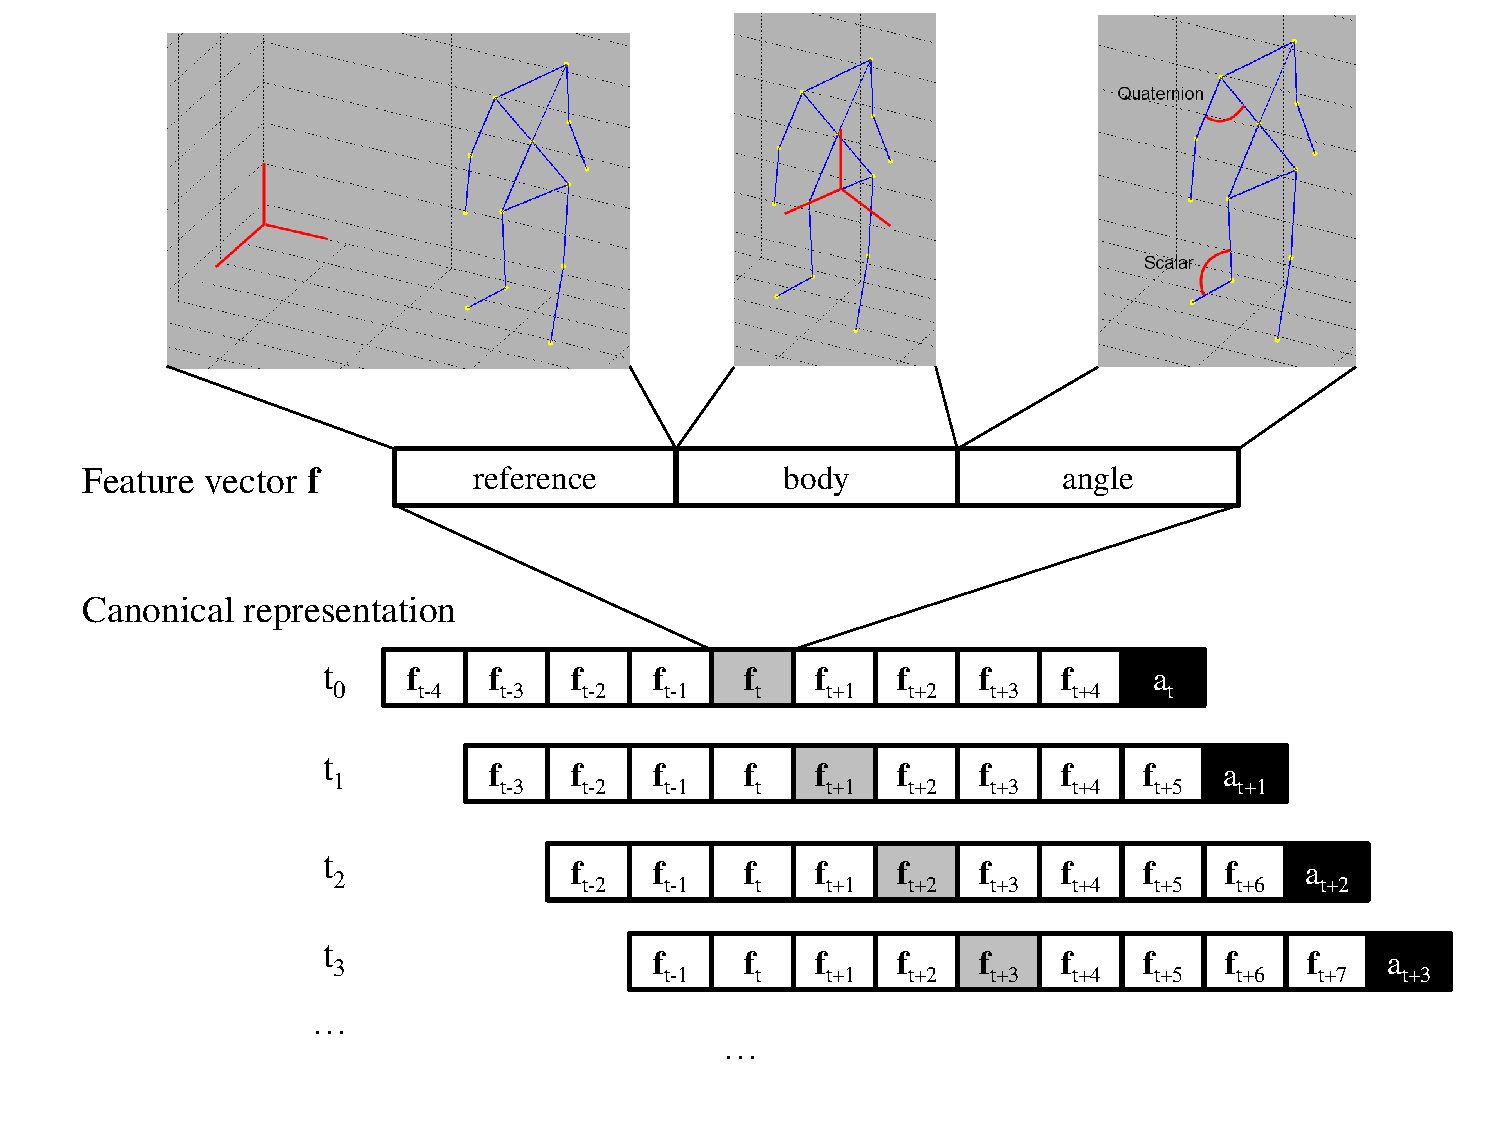
\includegraphics[width=\linewidth]{chap_AR/features}
\caption{An example of 10 feature vectors in canonical representation.}
\label{fig:canonical}
\end{figure}

The intuition behind the canonical representation is that an agent's actions are continuous and, hence, defined not only by the current values but also by the values in a certain time span. 
%Window length is chosen manually; long window length may lead to high 
So far, the features were expressed in corresponding coordinate systems at each time step $t$. However, the features $\mathbf{f}_i$ at time steps $i \not= t$ in the canonical representation can be expressed in the coordinate system belonging to the feature at time step $t$. This explicitly captures the changes between time steps within the interval. 





\subsection{Activity Recognition Model}
\label{sec:ArModel}
%\subsection{Results}
Once feature vectors are represented in the canonical form, it is possible to apply standard techniques for supervised classification, including feature selection, feature discretization, model learning, $k$-fold cross-validation, etc. The thesis will not delve into the details of the machine-learning algorithms. Any algorithm that supports numerical features can be applied to canonical representation, including SVMs, random forest, AdaBoost, decision trees, neural networks, multi-layer perceptrons, and others.

An important note considers $k$-fold cross-validation. Overlapping windows have a large degree of similarity and hence straight-forward $k$-fold cross-validation may produce an optimistic estimate of model performance. A better approach is to use folds that correspond to different sets of measurements or even different agents. For example, if the available dataset contains measurements of five agents, it makes sense to run {\it k-agent} cross-validation, where the model is trained on four agents and tested on the fifth.  The procedure is repeated for each agent and results are averaged.

%Activity recognition may be enhanced by appending A previous activities as recognized by the classifier to the attribute vector. This is particularly relevant in the first case where only a single set of attributes is used. The danger of appending previous activities is that the machine learning algorithm may learn that the current activity is always the same as the previous one, since this will often be the case. The problem may be circumvented by having two classifiers CA and C0. CA’s attribute vector contains A previous activities as recognized by C0. C0’s attribute vector does not contain any previous activities. This way even if CA gives a lot of weight to previous activities, the previous activities as recognized by C0 will change, as C0 is not burdened with CA’s inertia.

%
%==========================================================================================
%
\section{Reducing Spurious Activity Transitions}
\label{sec:ar:spurious}

\index{spurious activity transitions}
\index{noise removal}
An activity-recognition model classifies each window into one of the predefined activities; however, regardless of our efforts, it may still mislabel activities. The model usually mislabels single moments or short intervals more often than longer intervals. Activity recognition can be improved by taking into account the continuity of activities, for example, the agent cannot switch between walking and lying every tenth of a second. Such transitions between activities that do not occur in reality, but are caused by mislabeling, are considered spurious. 

One approach to enhancing the activity recognition model is to the extend feature vector with $k$ previous activities as recognized by the classifier. This leads to a potential problem, namely, the machine-learning algorithm may learn that the current activity is always the same as the previous one, since this is often the case. The problem may be circumvented by having two activity recognition models $\theta_A$ and $\theta$, where $\theta_A$'s attribute vector does not contain any previous activities, and $\theta$'s attribute vector contains $k$ previous activities as recognized by $\theta_A$. This way, even if $\theta$ heavily weights previous activities, those  recognized by $\theta_A$ will change, as $\theta_A$ is not biased with $\theta$'s inertia.

Based on the above intuition, we introduce two candidate approaches for reducing spurious activity transitions: sequential grammar-based classifier (SGBS) and hidden Markov models (HMM).  The input to these models is a sequence of actions $\mathbf{a}$ labeled by an activity recognition model $\theta_A$. 
\begin{definition}
\index{action!action sequence}
	\emph{Activity sequence} $\avec{T}$ is a totally-ordered sequence of $T$ actions s.t. $\avec{T}=\{a_t; 1 \leq t \leq T\}$.
\end{definition}
\noindent
The goal is to assign the best possible sequence of actions $\mathbf{a}'$ given a criterion and a sequence of input actions $\mathbf{a}$, often referred to as an observation sequence.


\subsection{Sequential Grammar-Based Classifier}

\index{sequential grammar-based classifier}
A sequential grammar-based classifier, introduced by \cite{Goshorn2001}, classifies an observed activity sequence $\mathbf{a}$ to the behavior which it most closely resembles. The similarity is defined in terms of the transformation cost of a sequence into a syntactically correct sequence belonging to that behavior. 

Suppose there is a set of $n$ possible behaviors $\mathbf{b}_i \in \mathbb{B}$, $1 \leq i \leq n$. A behavior $\mathbf{b}_i$ consists of a sequence of actions $a \in \mathbb{A}$ and is generated with a corresponding finite state machine $M_i(\mathbb{A}, S, s_o, \delta, F)$, where $\mathbb{A}$ is the input alphabet (activities), $S$ is a finite, non-empty set of states, $s_0$ is an initial state, $\delta: S \times \mathbb{A} \rightarrow S$ is state-transition function, and $F$ is the set of final states.


Suppose you want to classify an observation sequence $\avec{k}=\{a_1, a_2, ..., a_k\}$. If $\avec{k}$ is recognized by any of the automata $M_i$, then it is classified as behavior $\mathbf{b}_i$. If it is not, then it must be edited into a sequence that is. In order to do so, a new automaton $M'_i$ is created, which is able to parse unrecognizable sequence $\avec{k}$ by transforming any symbol within its alphabet, but with an associated cost, as follows. There are two operations that are used for transformations: substitution and deletion. Let $S(a_i, a_j)$ denote the operation of substituting an input symbol $a_i$ with $a_j$, and let $D(a_i)$ denote the operation of deletion of symbol $a_i$. Denote edit costs as $c_S(a_i, a_j)$ and delete cost $c_D(a_i)$, respectively. 

In order to utilize the performance of the classifier $\theta_A$, we use its performance measures obtained from its confusion matrix. The error rate for mislabeling an activity $a_i$ with $a_j$ is relevant for assigning the cost of substituting action $a_i$ with $a_j$. Therefore, to derive $c_S(a_i, a_j)$, we simply invert the probability $\Prob\{a_i|a=a_j\}$ from the confusion matrix:
\begin{equation}
\label{eq:sgbc}
c_S(a_i, a_j) = \frac{1}{\Prob\{a_i|a=a_j\}}.
\end{equation}

Similarly, the cost for deleting the action $a_i$ is defined inversely proportional to the inherent probability that classifier $\theta_A$ labels $a_i$ with true activity correctly. The deletion cost $c_D(a_i)$ is:
\begin{equation}
\label{eq:sgbc}
c_D(a_i) = \frac{1}{\Prob\{a_i|a=a_i\}}.
\end{equation}

Suppose, that in order to transform the action sequence $\avec{k}$ into a behavior $\mathbf{b}_i$, there need to be $n_S(a_i, a_j)$ substitutions of $a_i$ with $a_j$ and $n_D(a_i)$ deletions of $a_i$. Then, the distance $d(\avec{k}, \mathbf{b}_i)$ between the action sequence $\avec{k}$ and a behavior $\mathbf{b}_i$ is given by Equation~(\ref{eq:sgbc}):
\begin{equation}
\label{eq:sgbc}
d(\mathbf{a}, \mathbf{b}_i) = \sum_{i=0}^{|\mathbb{A}|} \sum_{j=0}^{|\mathbb{A}|} c_S(a_i, a_j) n_S(a_i, a_j) + \sum_{i=0}^{|\mathbb{A}|} c_D(a_i) n_D(a_i).
\end{equation}

The action sequence $\avec{k}$ is classified as a behavior $\mathbf{b}_i$ represented by a finite state machine $M_i'$ that outputted the smallest distance:
\begin{equation}
\label{eq:sgbc-argmin}
\mathbf{a} = \argmin{\mathbf{b}_i \in \mathbb{B}} d(\mathbf{a}, \mathbf{b}_i).
\end{equation}

In general, the lengths of behaviors $\mathbf{b}_i$ and action sequence $\mathbf{a}$ need not be be the same (although the lengths of behaviors $\mathbf{b}_i$ should be in to avoid length normalization). 
To avoid this problem,
%we can initialize one behavior $b$ for each action from $\mathbb{A}$. Then, given the input sequence $\mathbf{a}$, 
we use the overlapping sliding windows of length $|\mathbf{b}|$ and assign the classified behavior to the activity at the selected window index.



\subsection{Hidden Markov Models} 
\label{sec:ar:hmm}

\index{hidden Markov models}
Hidden Markov model (HMM) is a temporal probabilistic model with two embedded stochastic processes: a hidden process $Q$ that can be observed only through another visible process $O$. Each state has state-transition probabilities, which are visible, and a probability distribution over the possible values of $\mathbb{A}$. The key assumption is that the current hidden state of the agent is affected only by its previous state.  

A hidden Markov model $\theta(\mathbb{H}, \mathbb{A}, \delta, \nu, \pi)$ is characterized by the following:
\begin{itemize}
	\item $\mathbb{H}=\{h_i\}$ is a set of $N$ hidden states, individual states are denoted as $\mathbb{H}=\{h_1, h_2, ..., h_N\}$, and the state at time $t$ as $Q_t$,
	\item $\mathbb{A} = \{a_j\}$ is a set of distinct observation symbols (that is, activities) per state,
	\item $\delta = \{\delta_{ij}\}$ is the state transition probability distribution, where 
		\begin{equation}
			\label{eq:hmm-a}
			\delta{ij} = \Prob\{q_{t+1} = s_j | q_t = h_i\}, 1 \leq i,j \leq N,
			\end{equation}
	\item $\nu = \{\nu_{j}(k)\}$ is the state observation probability distribution, where 
			\begin{equation}
			\label{eq:hmm-b}
			\nu_{j}(k) = \Prob\{a_k | q_t = h_j\}, 1 \leq j \leq N, 1 \leq k \leq M, 
			\end{equation}
	\item $\pi=\{\pi_i\}$ is the initial state distribution, where
			\begin{equation}
			\label{eq:hmm-pi}
			\pi_i = \Prob\{q_1 = h_i\}, 1 \leq i \leq N.
			\end{equation}
\end{itemize}
\noindent An example of a hidden Markov model with $N=4$ hidden states and $M=3$ observation symbols is shown in Figure~\ref{fig:hmm}. 

\begin{figure}[!h]
\centering
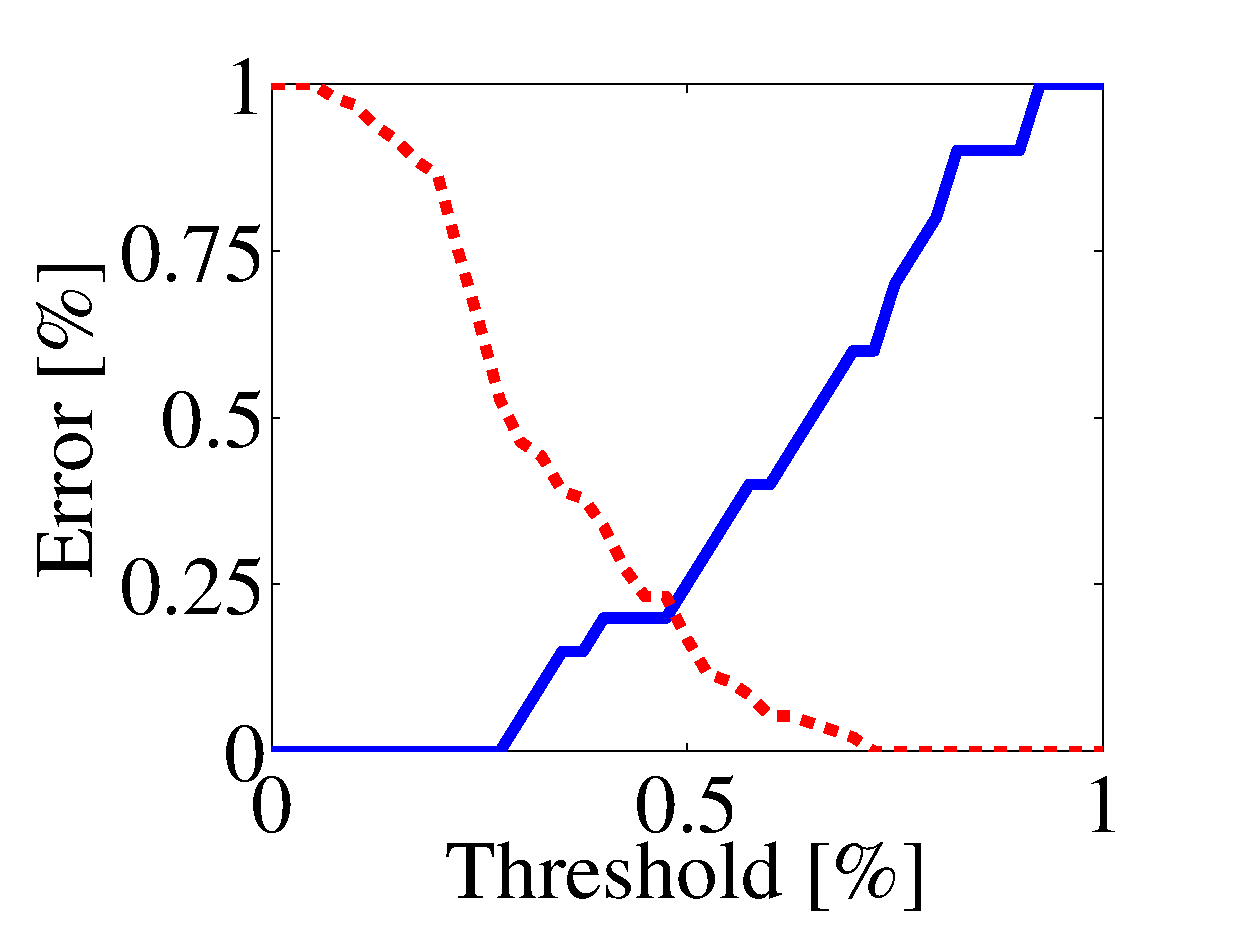
\includegraphics[width=\linewidth]{chap_AR/hmm}
\caption{An example of a hidden Markov model with four hidden states and three observation symbols.}
\label{fig:hmm}
\end{figure}

Given a learning set of observation sequences, there are two problems of interest that must be solved; that is, how to adjust model parameters so as to best describe agent behavior observation sequences, and, given a new observation sequence $\mathbf{a}^{(t)}$ and a model $\theta$, how to choose a corresponding state sequence $\mathbf{s} = \{q_i=h_j | 1 \leq i \leq t, 1 \leq j \leq M\}$, that best explains the observations.

%Consider a model $\theta$ characterized with $N$ hidden states, denoted as $S1, S2, …, SN$. Let aij denote state transition probability from state Si to Sj and let πi denote initial state distribution of state Si. Denote M as the number of distinct output symbols s1, s2, …, sm and output symbol distribution in state j as bj(k). Then, given appropriate values N, M, aij, πi, and bj(k), the HMM can be used as generator of output sequence s=s1s2s3…sk.

The first problem, where the goal is to adjust model parameters in order to maximize observation sequence probability, has no optimal solution. Parameters can be locally maximized with the Baum-Welch method~\citep{Baum1970}, which maximizes the likelihood of the training set. Instead of calculating the required state transitions from the observations, it iteratively estimates the parameters. The method starts with arbitrarily chosen values and then computes the expected frequencies by weighting the observed sequences over the current model probabilities. The expected frequencies substitute the old parameters and the procedure iterates until converging on a local maximum. 

The second problem, {\it uncovering} the hidden part of the model, is solved with the Viterbi algorithm~\citep{Viterbi1967}, which assumes that the output symbols in observation sequence $\mathbf{a}$ correspond to hidden state sequence $\mathbf{h}$. It finds the optimal state sequence $\mathbf{h}$ for the given observation sequence $\mathbf{a}$ in terms of maximizing the expected number of correct states, which is achieved with dynamic programming.

Suppose the task is to classify an observation sequence $\mathbf{a}$. First, an HMM model $\theta$ is created from the learning set of observations with the Baum-Welch method. Then, the Viterbi algorithm applied on model $\theta$ and observation sequence $\mathbf{a}$ returns the most probable hidden state sequence $\mathbf{h}$. In the last step, we take into account the $\theta$'s state observation probability distribution $\nu$ to assign the most probable symbol to each state; that is, it is assumed that a hidden state corresponds to the activity that is most likely observed in that state.

%
%==========================================================================================
%
\section{Compound-Activity Recognition}
\label{sec:ar:interactions}

\index{activity!compound activity}
We use the term compound activity to describe behavior within an activity sequence. %; that is, it describes behavior of an agent in a longer time interval 
Activities, in particular atomic actions, are mainly used as behavior primitives describing the most elementary behavior aspects, while compound activities describe higher-level behavior aspects, usually spanned over longer periods of time.

\begin{definition}
\label{def:compound_activity}
\index{interaction}
	\emph{Compound activity} $b_k \in \mathbb{B}$ describes an activity sequence $\avec{k}$ as behavior caused by an agent in a particular situation limited by time span $1 \leq t \leq k$ that explains activities $a_1, ..., a_k$, where $\mathbb{A}$ is a set of possible activities.
\end{definition}

The main difference between activities and compound activities is in the mapping function: an activity is assigned from observation vector(s), that is, $f: \mathbb{R}^{|\mathbf{x}|} \rightarrow \mathbb{A}$, while a compound activity is assigned from an activity sequence, that is, $g: \mathbb{A}^{|\avec{k}|} \rightarrow \mathbb{B}$. Given a set of possible compound activities $\mathbb{B}=\{b_i\}, 1 \leq i \leq K$, the goal is to classify an activity sequence $\mathbf{a}$ into one of the activities from $\mathbb{B}$.

For this task, we utilize hidden Markov models introduced in the previous section. The idea is to segment the learning set by different behavior types and to create an HMM model $\theta_i$ for each of the behaviors $b_i \in \mathbb{B}, 1 \leq i \leq K$.

Next, we compute the probability of the sequence $\mathbf{a}$ given a model $\theta_i$, that is, $P[a|\theta_i]$. The straightforward approach through enumerating every possible state sequence of length $T=|\mathbf{a}|$ involves the order of $2TN^T$ calculations~\citep{KollerFriedman2009}, which is computationally unfeasible even for small values of $N$ and $T$, for example, $N=5$ states and $T=100$ requires $~10^{72}$ calculations. A more efficient procedure, denoted as the forward-backward algorithm~\citep{Rabiner1989}, first computes a set of forward probabilities that predicts the likelihood of ending up in any particular state given the first $t$ observations in the sequence $\mathbf{a}$. In the second pass, the algorithm computes a set of backward probabilities that predicts the likelihood of the remaining observations given any starting point $t$. These two probability distributions can then be combined to obtain the distribution over states at any specific point in time given the entire observation sequence. The reader is referred to \cite{KollerFriedman2009} for details.

Finally, the atomic action sequence $\mathbf{a}$ is classified as the behavior $b_i$ that outputted the highest probability $\Prob\{\mathbf{a}|\theta_i\}$:
\begin{equation}
\label{eq:hmm-max}
\argmax{b_i \in \mathbb{B}} \Prob\{\mathbf{a}|\theta_i\}.
\end{equation}

%
%==========================================================================================
%
\section{Recognition of Agent-Agent Interactions}
\label{sec:ar:interactions}
\index{activity!compound activity}
The previous sections were mainly focused on single-agent behavior. In order to assess all the behavior aspects, some domains require recognition of interactions among agents.

\begin{definition}
\label{def:observation_vector}
\index{interaction}
	\emph{Interaction} between agents $A$ and $B$ or interactive behavior $\chi_{i, j}(\tuple{\mathbf{a}_A,\mathbf{a}_B}) \in \mathbb{I}$ is behavior in time span $i \leq t \leq j$ that explains activity sequences $\mathbf{a}_A$ and $\mathbf{a}_B$ that correspond to activity sequence of the agent $A$ and agent $B$, respectively. $\mathbb{I}$ is a set of possible interactions.
\end{definition}

\noindent In other words, an interaction describes joint behavior of two agents in a specific time span. 

\index{hidden Markov models!coupled hidden Markov models}
This section demonstrates an approach for interaction recognition based on coupled hidden Markov models (CHMMs), which are briefly described below. The reader is referred to \cite{Brand} for details. The observation sequence $\hat{\mathbf{a}}=\tuple{\mathbf{a}_A, \mathbf{a}_B}$ consists of two activity sequences, namely $\mathbf{a}_A$ of agent $A$ and $\mathbf{a}_B$ of agent $B$, when they are within some predefined radius $R$. The CHMMs are able to model complex, interactive behavior by two HMM chains, where the hidden states from one chain directly impact the hidden states from the other chain. 

Figure~\ref{fig:CHMMs} illustrates a CHMM for a pair of action traces with length $l=3$. The current state $Q_t^A$ of agent $A$ is affected by both its previous state $Q_{t-1}^A$ and previous state $Q_{t-1}^B$ of the agent $B$ (similarly $Q_t^B$ is affected by $Q_{t-1}^B$ and $Q_{t-1}^A$). Each state $Q_i$ also impacts the corresponding observation state $Y_t$. 
For example, if agent $A$ moves toward agent $B$, the next state of the latter takes this into account and produces a corresponding atomic action, for example, an avoidance maneuver. 

\begin{figure}[!ht]
\centering
\includegraphics[width=0.5\linewidth]{chap_AR/chmm}
\caption{An example of CHMM for a pair of action traces with length $T=3$.}
\label{fig:CHMMs}
\end{figure}

Similarly to the previous section, we create a CHMM model $\hat \theta_i$ for each interaction $\chi_i$ from the set of possible interactions $\mathbb{I}$. For an observation sequence $\hat{\mathbf{a}}$, the posterior probability is computed given the model $\hat \theta_i$ using slightly modified standard HMM algorithms. The reader is referred to \cite{Brand} and \cite{KollerFriedman2009} for details.
Finally, the interaction is classified by the model that outputs the highest probability $\Prob\{\hat{\mathbf{a}}|\hat \theta_i\}$:
\begin{equation}
\label{eq:chmm-max}
\argmax{\chi_i \in \mathbb{I}} \Prob\{\hat{\mathbf{a}}|\hat \theta_i\}.
\end{equation}


\section{Summary and Discussion}
This chapter addressed the activity recognition from sensor data, where considerable amount of noise is present. We introduced a pipeline-based approach, ARPipe, that includes noise removal, feature vector construction, activity recognition classifier, and spurious activity transition removal. The noise removal as well as feature vector construction steps were demonstrated on location-based sensors, which provide significantly less accurate measurements compared to location sensors used in related work \citep{Sukthankar2005, Qian2004}. Since real locations, that is, true locations of a moving object, were infeasible to obtain, the noise removal was evaluated indirectly in \citep{Kaluza2009Glajenje, Lustrek2009Behavior}, where it proved beneficial. The removal of spurious activity transitions was investigated in \citep{Kaluza09Reducing}, where HMM approach achieved better results. In summary, the main two novelties presented in this chapter are activity recognition from noisy location sensors, and the ARPipe, which represents a comprehensive approach to activity recognition.

ARPipe provides the fist step to anomalous and suspicious behavior detection by recognizing behavior primitives, that is, activities. Additional approaches, such as compound activity recognition and recognition of agent interactions, help us to recognize more complex behaviors. The next chapter will discuss how to encode and evaluate such behavior components.





\newpage \thispagestyle{empty}

%!TEX root = thesis.tex

%
%==========================================================================================
%
\chapter{Behavior Signatures}
\label{chap:signatures}

\index{behavior signature}
This chapter discusses how to encode a sequence of actions into a behavior signature. It introduces a novel presentation denoted as a spatio-activity matrix, demonstrates a  visualization technique, and proposes a feature extraction approach.

%
%==========================================================================================
%
\section{Definitions}
In Chapter~\ref{chap:activity_recognition}, we transformed a sequence of observation vectors to a higher-level description of behavior primitives. This chapter discusses how to efficiently encode the sequence of behavior primitives in order to perform additional analysis and effectively visualize the data. By effective visualization, we aim at a presentation that allows humans to quickly compare various behavior patterns and to find the main differences among them.

First, we define static points in the environment that refer to significant locations, specific spatial areas, or regions of partitioned space (for example, squared partitioning).
\begin{definition}
\label{def:landmark}
\index{static landmark}
	\emph{Static landmark} $s$ is a point in the environment that remains fixed over the observed period of time. A set of static landmarks in the environment is denoted as $\mathbb{S}=\{s_i\}$.
\end{definition}
\noindent 

Next, given a set of static landmarks $\mathbb{S}$ and a set of activities $\mathbb{A}$, the behavior can be described in landmark-activity state space $\mathbb{S} \times \mathbb{A}$.
The behavior can be then represented as a trajectory through the landmark-action state space as follows. 

\begin{definition}
\label{def:behavior_trace}
\index{behavior trace}
	\emph{Behavior trace} $\mathbf{b}=\{\tuple{a, s}_t\}, 1 \leq t \leq T$ is a sequence of tuples in which each tuple $\tuple{a,s}_t$ indicates the environmental state $s$ and the activity $a$ being performed at this state at time step $t$.
\end{definition}




%
%==========================================================================================
%

\section{Spatio-Activity Matrix}

\index{feature extraction}
This section introduces a behavior-trace encoding that captures activity distributions, landmark distribution, distribution of activities over landmarks, and distribution of landmarks over activities. 

Consider a set $\mathbb{A}=\{a_1, a_2, ..., a_M\}$ of predefined activities and a set $\mathbb{S}=\{s_1, s_2, ..., s_K\}$ of static landmarks where the agent can be present. Let $\mathbf{v}_t$ denote a spatio-activity vector of size $M+K$ at time step $t$. The first $M$ elements correspond to $M$ activities in $\mathbb{A}$ and the last $K$ elements correspond to static landmarks in $\mathbb{S}$; that is, $i$-th element corresponds to $a_i$ if $i\leq M$ or $s_{i-M}$ if $M < i \leq K$. 

A tuple $(a, s)_t$ is then transformed to the spatio-activity vector with Equation~(\ref{eq:spatio-activity-vector}), which assigns a binary value to $i$-th element of the vector: 1, if the activity is equal to $i$-th activity in $\mathbb{A}$ or if the landmark is equal to landmark at position $i-M$ in $\mathbb{S}$; 0, otherwise.
\begin{equation}
\label{eq:spatio-activity-vector}
\index{spatio-activity matrix}
\mathbf{v}_{t(i)} = \left\{
\begin{array}{l l}
 1 & \quad ;\mbox{if } a=a_i, 1 < i \leq M \mbox{ or } s=s_{i-M}, M < i \leq K,\\
 0 & \quad ;\mbox{otherwise.}\\ \end{array} \right. \
\end{equation}
\noindent A spatio-activity vector is basically a binary representation of activities and landmarks present in a tuple.

Suppose we have two spatio-activity vectors $\mathbf{v}_i$ and $\mathbf{v}_j$. Let $\mathbf{t}(\mathbf{v}_i, \mathbf{v}_j)$ denote a transition vector from the spatio-activity vector $\mathbf{v}_i$ to $\mathbf{v}_j$ as an indication of a change constrained by $\|\mathbf{t}(\mathbf{v}_i, \mathbf{v}_j)\|=1$:
\begin{equation}
\mathbf{t}(\mathbf{v}_i, \mathbf{v}_j) = \neg(\mathbf{v}_j \rightarrow \mathbf{v}_i),
\label{eq:transition}
\end{equation}
\noindent
where operator `$\rightarrow$' is binary implication and `$\neg$' is binary negation.

Now suppose we want to encode the behavior trace $\mathbf{b} = \{(a,s)_t\}, 1 \leq t \leq T$. First, we assign a new vector $\mathbf{v}_t$ to each tuple $(a,s)_t$. Let $\mathbf{M}(\mathbf{b})$ denote the spatio-activity matrix, where the dynamics of a person in the given behavior trace $\mathbf{b}$ is captured:
\begin{equation}
\mathbf{M}(\mathbf{b}) = \mathbf{v}_1  {\mathbf{v}_1}^\intercal + \sum_{t\in[2, ..., T]} [\mathbf{v}_t {\mathbf{v}_t}^\intercal + \mathbf{t}(\mathbf{v}_{t-1}, \mathbf{v}_t) \mathbf{t}(\mathbf{v}_{t-1}, \mathbf{v}_t)^\intercal]
\label{eq:matrix}.
\end{equation}
\noindent
At this step, the spatio-activity matrix $\mathbf{M}$ registered element frequency in a spatio-activity vector and their transitions. In order to make $\mathbf{M}$ comparable to other matrices constructed from behavior traces of different lengths, the matrix $\mathbf{M}$ must be normalized.

Define $norm(\mathbf{M})$ as an operation that normalizes the values of the matrix $\mathbf{M}$ to the interval $[0, 1]$. The $norm(\mathbf{M})$ is defined for an element $\mathbf{M}_{i,j} \in \mathbf{M}$ by the expression
%
\begin{equation}
\mathbf{M}_{i, j} =  \left\{
\begin{array}{l l}

 \frac{\mathbf{M}_{i,j}}{\sum_{k=1}^{M} \mathbf{M}_{k,k}} & ; i = j \wedge i \leq M  \\

 \frac{\mathbf{M}_{i,j}}{\sum_{k=M+1}^{M+K} \mathbf{M}_{k,k}} & ; i = j \wedge i > M  \\

 \frac{\mathbf{M}_{i,j}}{\sum_{\substack{k=1\\l=1\\l\not = k}}^{M} \mathbf{M}_{k,l}} & ; i \neq j \wedge i \leq M \wedge j \leq M  \\

 \frac{\mathbf{M}_{i,j}}{\sum_{\substack{k=M+1\\l=M+1\\l\not = k}}^{M+K} \mathbf{M}_{k,l}} & ; i \neq j \wedge i > M \wedge j > M  \\

 \frac{\mathbf{M}_{i,j}}{\sum_{k=M+1}^{M+K} \mathbf{M}_{i,k}} & ; i \leq M \wedge j > M  \\

 \frac{\mathbf{M}_{i,j}}{\sum_{k=1}^{M} \mathbf{M}_{i,k}} & ; i > M \wedge j \leq M  \\

\end{array}. \right. \
\label{eq:normalize}
\end{equation}
%
Intuitively, the matrix $\mathbf{M}$ consists of six regions as shown in Figure~\ref{fig:matrix-regions}.
\begin{figure}[!ht]
\centering
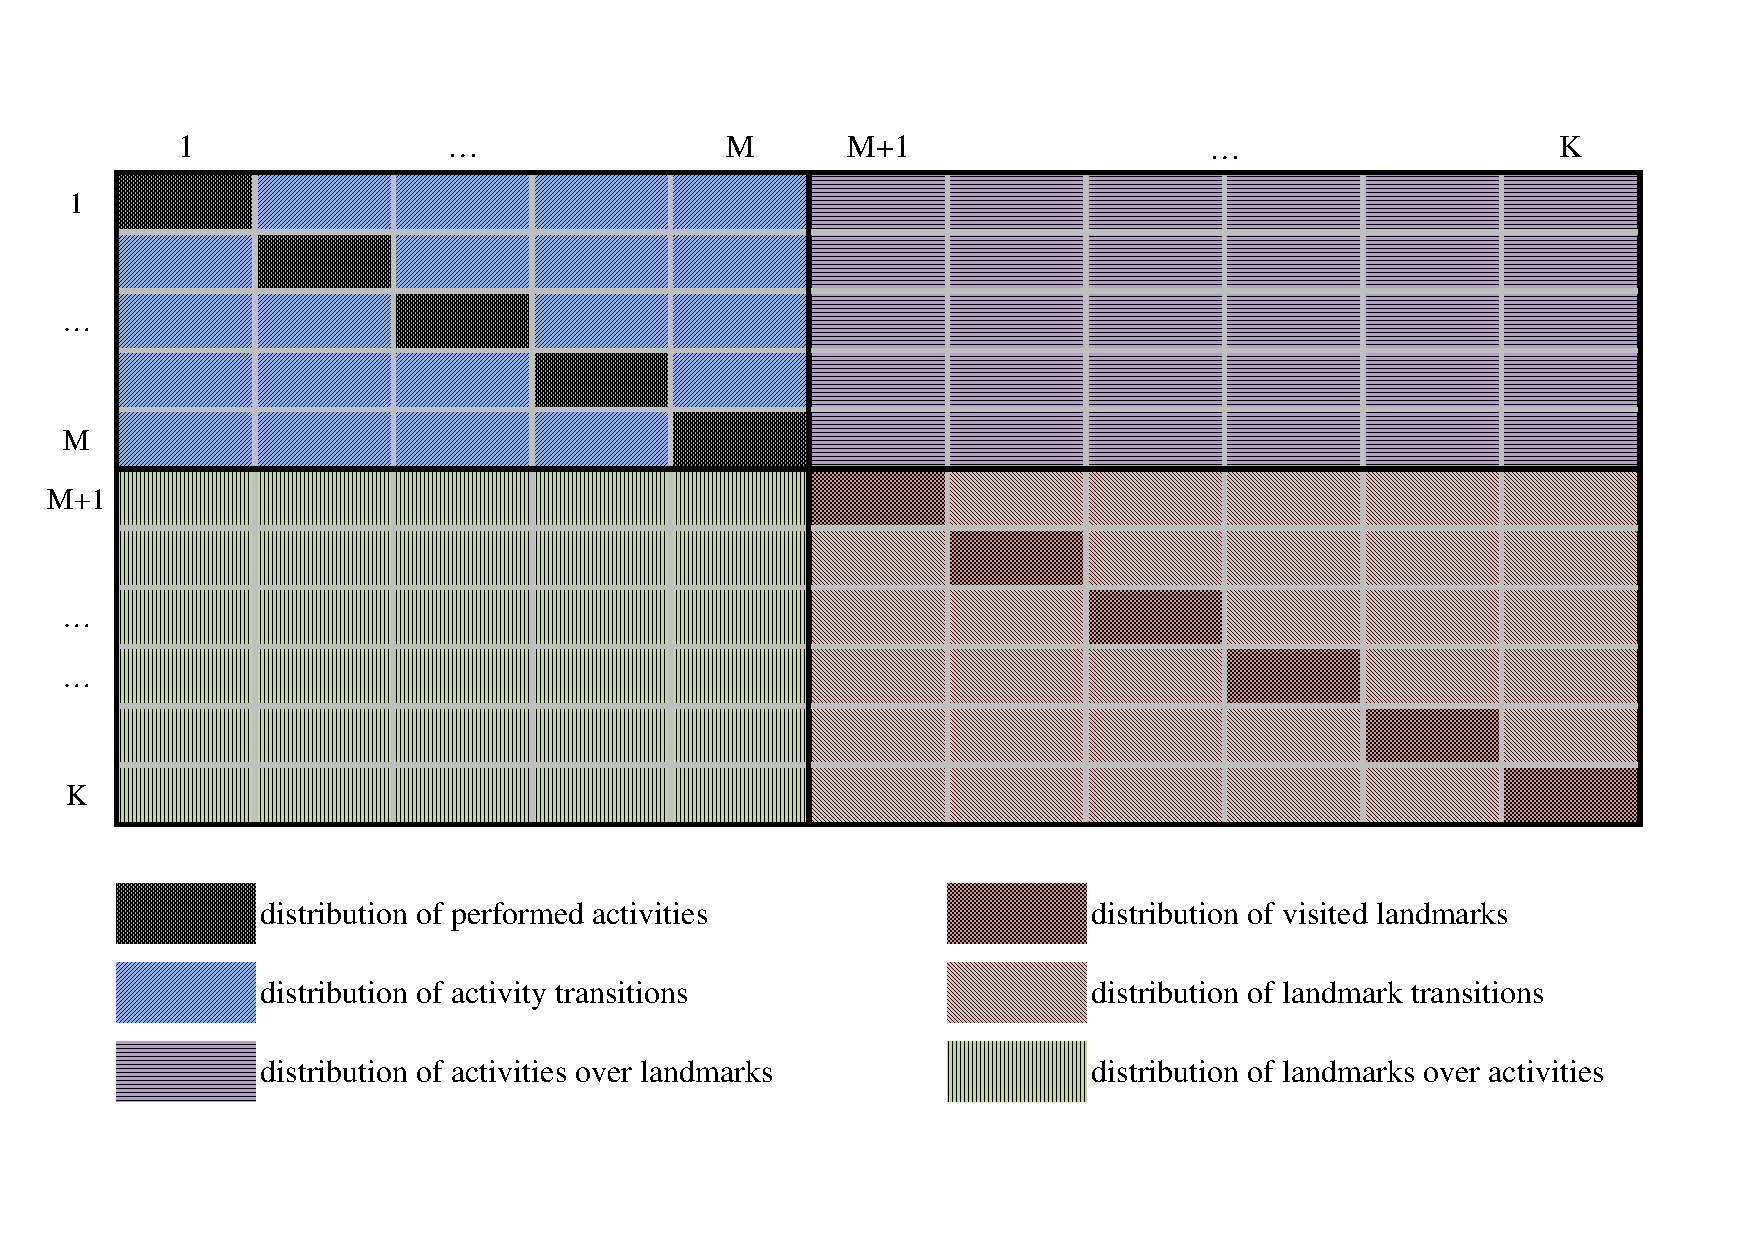
\includegraphics[width=\textwidth]{chap_BS/matrix}
\caption{Regions of spatio-activity matrix.}
\label{fig:matrix-regions}
\end{figure}
The interpretation of the regions is as follows: the activity-activity part (top left) includes the fractions of the time spent performing particular activities (diagonal elements) and the distribution of transitions between activities (non-diagonal elements); the spatio-spatio part (bottom right) includes the fractions of time spent at the particular landmarks (diagonal elements) and the distribution of transitions  between landmarks (non-diagonal elements); the activity-spatio part (top right) describes the distribution of activities over landmarks; and the spatio-activity part (bottom left) describes the distribution of landmarks over activities.

The complete spatial-activity construction procedure is described in Algorithm~\ref{alg:SA_matrix}. The input is a behavior trace $\mathbf{B}$. Each tuple $(a, s)_t \in \mathbf{B}$ is first transformed into the spatio-activity vector $\mathbf{v}_t$ using Equation~(\ref{eq:spatio-activity-vector}) and added to a temporary sequence of vectors $\mathbf{V}$. The sequence $V$ is then used to compute the spatio-activity matrix $\mathbf{M}$ using Equation~(\ref{eq:matrix}). Finally, the matrix $\mathbf{M}$ is normalized by Equation~(\ref{eq:normalize}).

\begin{algorithm}
\caption{Create spatio-activity matrix.}
\label{alg:SA_matrix}
\begin{algorithmic}
\REQUIRE behavior trace $\mathbf{b}=\{\tuple{a,s}_1,\tuple{a,s}_2,...,\tuple{a,s}_n\}$
\ENSURE normalized matrix $\mathbf{M}(\mathbf{b})$
\STATE $\mathbf{V}\gets \{\}$
\FOR {$\tuple{a,s} \in \mathbf{b}$}
\STATE $\mathbf{v} \gets sa\_vector({\tuple{a,s}}) $
\STATE $\mathbf{V} \gets \mathbf{V} \cup \mathbf{v} $
\ENDFOR
\STATE $\mathbf{M} \gets \mathbf{v}_1  {\mathbf{v}_1}^\intercal$
\FOR {$v_i \in \mathbf{V}$, $i>1$}
 \STATE $\mathbf{M} \gets \mathbf{M} +  \mathbf{v}_i{\mathbf{v}_i}^\intercal + \mathbf{t}_{i-1, i}  {\mathbf{t}_{i, i-1}}^\intercal$
\ENDFOR
%+ \sum_{i\in[1, ..., k]}( v_i*{v_i}^\intercal + t_{i-1, i} * {t_{i, i-1}}^\intercal)$
\STATE $norm(\mathbf{M})$
\end{algorithmic}
\end{algorithm}

%==========================================================================================

\subsection{Time Complexity Analysis}

The runtime complexity increases linearly with the behavior trace length $T$ and quadratically with the sizes of sets $\mathbb{A}$ and $\mathbb{S}$. First, $T(M+K)$ operations are required to transform each tuple to a spatio-activity vector. Next, there are $2(T-1)(M+K)$ operations to compute $T-1$ transition vectors using implication and negation on each pair of spatio-activity vectors. The next step builds the spatio-activity matrix, where each of vector-vector multiplications requires $2(M+K)$ operations that result in matrices. Matrix summarization requires $(M+K)^2$ steps, and is applied for each T. In total there are $2(M+K)+(M+K)^2+T(4(M+K)+(M+K)^2)$ operations. The normalization step can be implemented by pre-computing the six divisors and applying them on each element in the matrix. This requires $T(M+K+M^2+K^2+2(MK))$ operations in total. The overall time complexity, then, is $O(T(M+K)^2)$.

In practice, however, the behavior trace is a few orders of magnitude larger than the number of activities and landmarks; that is, $(M+K) << T$, which makes the computation of spatio-activity matrix dependent only on the behavior trace length $T$.


%==========================================================================================

\subsection{Visualizations}

Since the matrix $\mathbf{M}$ is normalized to the interval $[0, 1]$, it can be visualized with a color map. Figure~\ref{fig:Mmatrix} shows an example of such a matrix $\mathbf{M}$ visualization, where the color ranges from low frequency (blue) to high frequency (red); a warmer color represents a higher intensity (see the legend on the left-hand side). It shows a behavior matrix constructed from a daily behavior trace of a person for activities $\mathbb{A}=\{lying, sitting, standing\}$ and landmarks $\mathbb{S}=\{lounge, bedroom, kitchen, toilet\}$.

\begin{figure}[!ht]
\centering
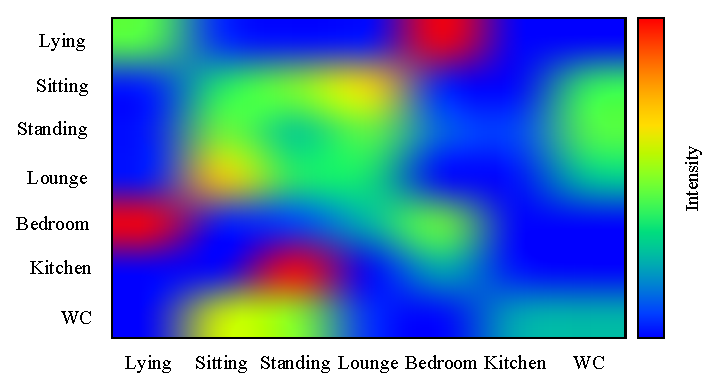
\includegraphics[width=0.9\textwidth]{chap_BS/spatial-activity-matrix}
\caption{Visualization of a daily spatio-activity matrix of one person. A warmer color represents a higher value.}
\label{fig:Mmatrix}
\end{figure}

Figure~\ref{fig:Mmatrix} can be interpreted as follows. There are three red squares that indicate a high ratio: $M_{bedroom, lying}$ indicates that lying is the prevailing bedroom activity;  $M_{kitchen, standing}$ indicates that standing is the prevailing kitchen activity; and $M_{lying, bedroom}$ indicates that lying is mostly carried out in the bedroom. Next, blue squares indicate activity absence; for example, $M_{kitchen, lying}$ and $M_{kitchen, sitting}$ indicate that lying and sitting rarely occurred in the kitchen. Diagonal elements in the bottom-right part of the table (that is, $M_{lounge, lounge}$, $M_{bedroom, bedroom}$, $M_{kitchen, kitchen}$, $M_{toilet, toilet}$) reveal that the person spent most of the time in the bedroom followed by the lounge and toilet, and almost no time in the kitchen.

The visualization is especially useful in a comparison of multiple behavior traces. A small change, for example, in the ratio between sleeping in the bed (being ill) and walking around the apartment (a healthy person), is rapidly propagated through the spatio-activity matrix and, therefore, one can quickly notice the change and the type of change at the same time.


%==========================================================================================

\subsection{Feature Extraction}
\label{sec:ba:PCA}

The behavior matrix can be directly fed into models for anomalous and suspicious behavior detection (discussed in Chapter~\ref{chap:detection}) by transforming the spatio-activity matrix $\mathbf{M}^{M+K, M+K}$ to a feature vector $\mathbf{m}$. Note that the vector $\mathbf{m}$ contains $(M+K)^2$ elements, and some of them rarely change in different behavior traces. The main idea, then, is to reduce the number of features to the most representative set. This section presents an approach based on dimensionality reduction technique denoted as principal component analysis.

\index{principal component analysis}
Principal component analysis (PCA) is an orthogonal linear transformation of possibly correlated variables onto a subspace. The choice of the $k$-dimensional projection subspace is made such that the projection distances have a minimal deformation: squares of the  $k$-dimensional subspace distances are as large as possible. By projecting the data onto the new coordinate system, the greatest variance emerges on the first coordinate (called the first principal component), while the second greatest variance emerges on the second coordinate, and so on.

Implementing PCA is the equivalent of applying Singular Value Decomposition (SVD) to the covariance matrix. Consider a set of spatio-activity matrices $\mathbb{M}=\{\mathbf{M}_i\}$, $1 \leq i \leq L$.
Each spatio-activity matrix $\mathbf{M}_i$ is unrolled into a vector $\mathbf{m}_i$. Then we construct a matrix $\mathbf{\widehat M}$, which consists of $L$ vectors $\mathbf{m}_i$, each unrolled from $\mathbf{M}_i$, $i=1...L$.

\begin{eqnarray}
\mathbf{\widehat M} = \begin{bmatrix}
		\mathbf{m}_1 \\
		\mathbf{m}_2 \\
		\vdots \\
		\mathbf{m}_L \\
	\end{bmatrix} = \begin{bmatrix}
		\mathbf{M}_{1,1} & \mathbf{M}_{1,2} & \cdots & \mathbf{M}_{1, (M+K)^2} & \\
		\mathbf{M}_{2,1} & \mathbf{M}_{2,2} & \cdots & \mathbf{M}_{2, (M+K)^2} & \\
		\vdots 			 &	\vdots			& \ddots & \cdots \\
		\mathbf{M}_{L,1} & \mathbf{M}_{L,2} & \cdots & \mathbf{M}_{L, (M+K)^2} & \\
	\end{bmatrix}
\end{eqnarray}

 The PCA proceeds as follows:  first, we compute the mean vector $\mathbf{\bar\mu}$ with $\mu_j$ elements, $1 \leq j \leq (M+N)^2$ with Equation~(\ref{eq:PCA-1}), and subtract the mean from $\mathbf{\widehat M}$ with Equation~(\ref{eq:PCA-2}), which gives us matrix $\mathbf{\widehat M}_z$ with zero mean.

\begin{equation}
\mu_j = {1 \over L} \sum_{k=1}^L \mathbf{M}_{k, j}, 1 \leq j \leq (M+N)^2
\label{eq:PCA-1}
\end{equation}

\begin{equation}
\mathbf{\widehat M}_z = \mathbf{\widehat M} - \begin{bmatrix}
		1 \\
		1 \\
		\vdots \\
		1 \\
	\end{bmatrix}_{L} \mathbf{\bar\mu}
\label{eq:PCA-2}
\end{equation}

Next, a matrix $\mathbf{C}$ of variances and covariances is computed with Equation~(\ref{eq:PCA-3}), where the diagonal elements $i = j$ are variances $\sigma_{ij}^2$ and the non-diagonal elements $i \neq j$ are covariances $\sigma_i\sigma_j$. 

\begin{equation}
\mathbf{C} = {1 \over L} \mathbf{\widehat M}_z \mathbf{\widehat M}_z^\intercal
\label{eq:PCA-3}
\end{equation}

Finally, $\mathbf{C}$ is decomposed into three matrices with SVD (Equation~(\ref{eq:PCA-4})). $\mathbf{S}$ is a diagonal matrix that stores singular values $\lambda_1, \lambda_2, ..., \lambda_n$. $\mathbf{U}$ and $\mathbf{V}$ are orthogonal matrices, while their column vectors are the so-called left and right eigenvectors of $\mathbf{C}$. 

\begin{equation}
\mathbf{C} = \mathbf{USV}^\intercal
\label{eq:PCA-4}
\end{equation}

When these eigenvectors multiply $\mathbf{\widehat M}_z$, the coordinates are shifted and rotated until they end up aligned with basis vectors. Note that PCA now re-expresses the data as a linear combination of its basis vectors, $\mathbf{\widehat M}_z\mathbf{V}$. $\mathbf{V}$ columns are found to produce the desired linear combinations. The first $\mathbf{V}$ column corresponds to the largest principal component, the second column corresponds to the second largest, and so on. These define the direction in which the variability of the original data set is maximized.

The transformed data now enable the use of anomalous and suspicious behavior detection models. All the behavior matrices $\{\mathbf{M}_i\} \in \mathbb{M}$, $1 \leq i \leq L$ are first expressed in the new coordinate system. When a new behavior matrix $\mathbf{M}_{L+1}$ is obtained, it is first expressed in the same system; the first components are subsequently used for further detection.
%As the first method we have chosen Local Outlier Factor algorithm because it has proven successful in several previous projects (literature?).


%
%==========================================================================================
%

\section{Summary and Discussion}
This chapter proposed a novel, efficient encoding denoted as spatio-activity matrix that is able to capture behavior dynamics in a specific time period using spatio-temporal features. We provided a visualization technique to compare different behavior patterns. We further provided a feature extraction technique based on principal component analysis to reduce the spatio-activity matrix dimensionality, which can be directly used in anomaly detection algorithms. Compared to related work based on HMMs~\citep{Monekosso}, the behavior patterns dynamics is expressed explicitly and can be visualized. Moreover, in contrast to research based on rule induction~\citep{Lee04daily,Lymberopoulos}, the presentation does not extract the exact behavior patterns, which leads to better generalization.

The obtained spatio-temporal features or their principal componentes will be used in the next chapter, which evaluates behavior patterns to perform anomalous and suspicious behavior detection. The spatio-temporal matrix can be constructed on various time intervals, such as hours, days, weeks, which provides different behavior encoding granularities; Section~\ref{sec:combine} discusses how to combine such evaluations. Also, the approach was demonstrated on spatio-temporal feature space, but in general, it can be applied on other feature spaces as well, which is an interesting direction for further investigations.

%


% \section{Behavior Trace Visualization}


% %---------------------------------------------------------------------

% \begin{algorithm}
% \caption{Trace visualization.}
% \label{alg:SA_matrix}
% \begin{algorithmic}
% \REQUIRE behavior trace $B=\{(a,s)_1,(a,s)_2,...,(a,s)_n\}$
% \ENSURE normalized matrix $M(B)$
% \STATE $V\gets \{\}$
% \FOR {$e \in S$}
% \STATE $v \gets sa\_vector(e) $
% \STATE $V \gets V \cup v $
% \ENDFOR
% \STATE $M \gets v_1 * {v_1}^\intercal$
% \FOR {$v_i \in V$, $i>1$}
%  \STATE $M \gets M +  v_i*{v_i}^\intercal + t_{i-1, i} * {t_{i, i-1}}^\intercal$
% \ENDFOR
% %+ \sum_{i\in[1, ..., k]}( v_i*{v_i}^\intercal + t_{i-1, i} * {t_{i, i-1}}^\intercal)$
% \STATE $norm(M)$
% \end{algorithmic}
% \end{algorithm}

% \begin{figure}[!ht]
% \centering
% 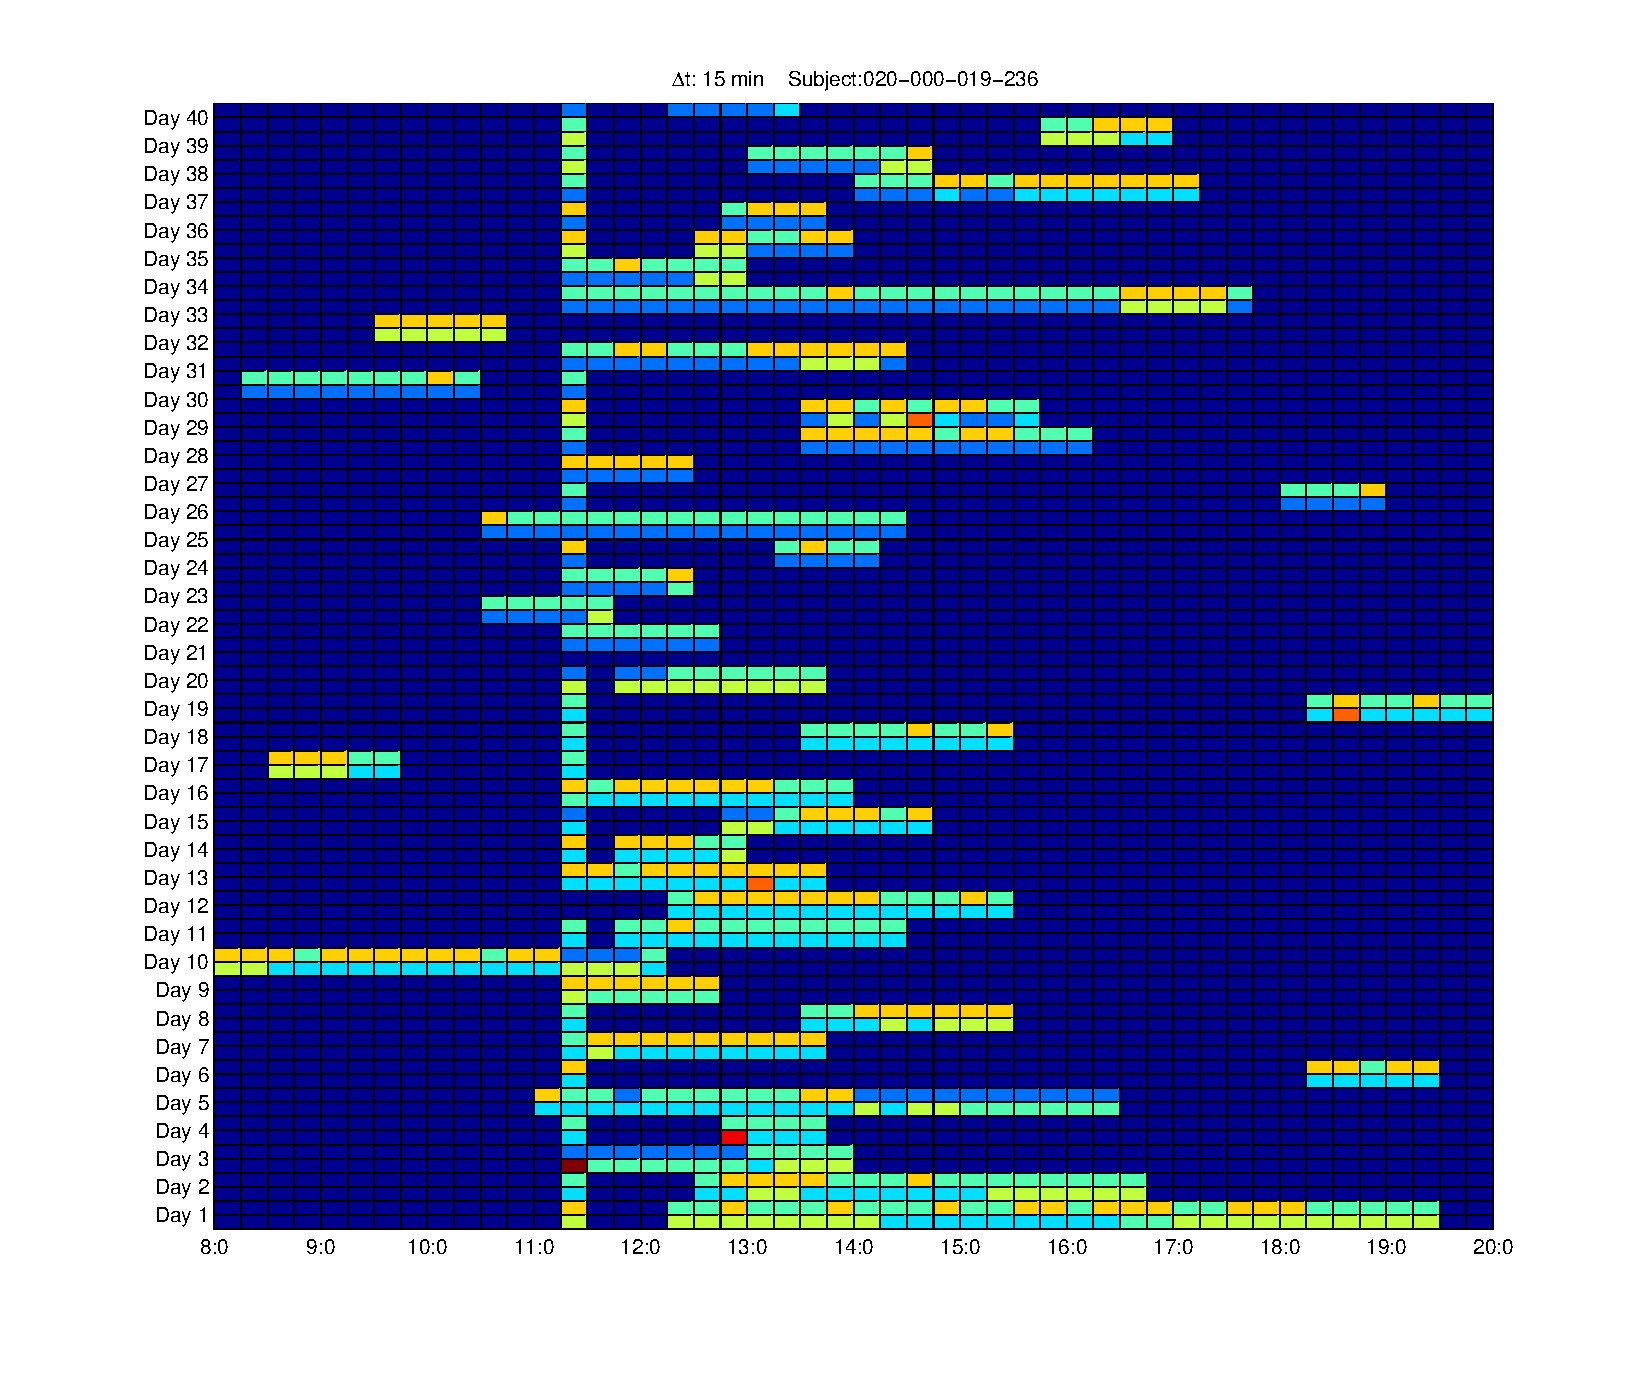
\includegraphics[width=\textwidth]{chap_BS/days}
% \caption{An example of monthly visualization.}
% \label{fig:month-signature}
% \end{figure}

% %---------------------------------------------------------------------

% \begin{algorithm}
% \caption{Behavior trace over time intervals.}
% \label{alg:SA_matrix}
% \begin{algorithmic}
% \REQUIRE behavior trace $B=\{(a,s)_1,(a,s)_2,...,(a,s)_n\}$
% \ENSURE normalized matrix $M(B)$
% \STATE $V\gets \{\}$
% \FOR {$e \in S$}
% \STATE $v \gets sa\_vector(e) $
% \STATE $V \gets V \cup v $
% \ENDFOR
% \STATE $M \gets v_1 * {v_1}^\intercal$
% \FOR {$v_i \in V$, $i>1$}
%  \STATE $M \gets M +  v_i*{v_i}^\intercal + t_{i-1, i} * {t_{i, i-1}}^\intercal$
% \ENDFOR
% %+ \sum_{i\in[1, ..., k]}( v_i*{v_i}^\intercal + t_{i-1, i} * {t_{i, i-1}}^\intercal)$
% \STATE $norm(M)$
% \end{algorithmic}
% \end{algorithm}

% \begin{figure}[!ht]
% \centering
% 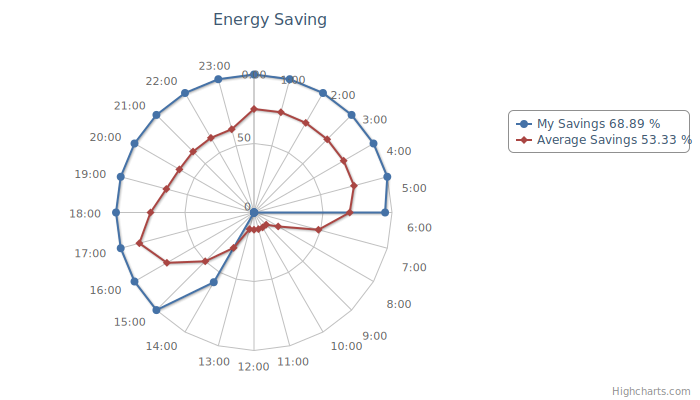
\includegraphics[width=\textwidth]{chap_BS/spider}
% \caption{An example of daily visualization.}
% \label{fig:spider}
% \end{figure}

\newpage \thispagestyle{empty}

%!TEX root = thesis.tex

%
%==========================================================================================
%
\chapter{Anomalous and Suspicious Behavior Detection}
\label{chap:detection}

This chapter discusses how to approach anomalous and suspicious behavior detection. It first formalizes the problem and shows how to optimally perform detection. It then discusses why optimal detection is not always possible, proves the lower error bound and discusses heuristics approaches. Finally, it describes how to design multi-view detectors and combine their evaluations. 

%
%==========================================================================================
%
\section{Detection Objectives}

Our focus is detection of deviant behavior patterns that might represent a security risk, health problem, or any other abnormal behavior contingency. Such patterns occur  infrequently; however, when they do occur, their consequences can be quite dramatic, and  often negatively. Typical examples include credit card fraud detection, cyber intrusions, industrial damage, etc. 

\index{feature extraction}
More formally, we define behavior pattern as follows:
\begin{definition}
\index{behavior pattern}
	\emph{Behavior pattern} $\bsig$ is a vector of features extracted from behavior trace $\mathbf{b}=\{(a, s)_t | 1 \leq t \leq T\}$.
\end{definition}
\noindent
The definition implies that a behavior pattern can be constructed from a behavior trace by an arbitrary function. The main idea is to introduce a set of features that effectively encodes the behavior trace, such as the spatio-activity matrix introduced in Chapter~\ref{chap:signatures}.


% is related to the lack of complete pos false alarms
%For example, 
\index{behavior!deviant behavior}
We use term \emph{deviant behavior} to refer to behavior that is either suspicious or anomalous and cast the deviant behavior detection problem in a statistical framework, which builds upon \cite{Helman1993} intrusion detection framework. This will help introduce rigorous notions, which are required later in the thesis, and allow future work to evolve toward broader objectives.

At time step $t$, we observe a behavior pattern $\bsig_t$, generated by a hidden stochastic process $H$. Now suppose that $H$ is a mixture of two auxiliary stochastic processes, namely the normal process $N$ and the suspicious process $S$, that correspond to a legitimate and a deviant behavior of an agent, respectively. The random variable $y_t=0$ if $\bsig_t$ is generated by $N$ and $y_t=1$ if $\bsig_t$ is generated by $S$. 
%Since an anomalous agent always emits an anomalous behavior pattern (and a legitimate agent a legitimate pattern), $y$ for a specific agent does not change over time. 
In reality, there can be many subprocesses contributing to both $N$ and $S$; that is, many legitimate agents with different behavior patterns or an agent with many legitimate and deviant behavior profiles. However, here we assume only a single $N$ and a single $S$ that capture all the variability. 

To this point, we have assumed that an observer is able to observe perfectly whether a behavior pattern is generated by $S$ or $N$. In practice, however, it may appear that a legitimate agent emits deviant behavior patterns (or vice-versa). An observer might be limited for various reasons, such as an inability to detect characteristic features, and noisy activity recognition models. Therefore, we relax this assumption as follows: a behavior pattern $\bsig_t$ is observed as generated by $N$ with the probability 
\begin{equation}
	n(\bsig_t) = \Prob\{H(t)=\bsig_t|y_t=0\},
\end{equation}
and as generated by $S$ with the probability 
\begin{equation}
	s(\bsig_t) = \Prob\{H(t)=\bsig_t|y_t=1\}.%= 1 - n(\bsig_t).
\end{equation}
Given the preceding assumption, that is, \emph{a priori} probability $\lambda$ that a behavior pattern is legitimate, the mixture distribution of a pattern $\bsig_t$ is
\begin{equation}
  \Prob\{H(t)=\bsig_t\} = \lambda n(\bsig_t) + (1-\lambda) s(\bsig_t).
\end{equation}
\noindent
Note that in most applications, $\lambda$ is close to 1, since deviant behavior patterns are rare, necessitating the application of modeling techniques such as those described in the next section.

We illustrate via a simple example the above-mentioned definitions and concepts. Suppose the behavior pattern consists of only two features, \emph{activity} and \emph{landmark}, and that the possible values for \emph{activity} are $\mathbb{A}=\{standing, lying\}$, while the possible values for \emph{landmark} are $\mathbb{S}=\{kitchen, bedroom\}$. Hence, the spatio-activity space can be presented by the set $\{\tuple{kitchen, standing}, \tuple{kitchen, lying}, \tuple{bedroom, standing}, \tuple{bedroom, lying}\}$ of ordered pairs.
Assume the following probability distribution on spatio-activity space for $1 \leq t \leq T$:
\begin{eqnarray*}
\Prob\{H(t)=\tuple{kitchen, standing}|y_t=0\} 	= n(\tuple{kitchen, standing}) &=& 0.950, \\
\Prob\{H(t)=\tuple{kitchen, lying}|y_t=0\}  	= n(\tuple{kitchen, lying}) &=& 0.020, \\
\Prob\{H(t)=\tuple{bedroom, standing}|y_t=0\}  = n(\tuple{bedroom, standing}) &=& 0.250, \\
\Prob\{H(t)=\tuple{bedroom, lying}|y_t=0\} 	= n(\tuple{bedroom, lying}) &=& 0.850,\\
\Prob\{H(t)=\tuple{kitchen, standing}|y_t=1\}  = s(\tuple{kitchen, standing}) &=& 0.020, \\
\Prob\{H(t)=\tuple{kitchen, lying}|y_t=1\}  	= s(\tuple{kitchen, lying}) &=& 0.900, \\
\Prob\{H(t)=\tuple{bedroom, standing}|y_t=1\}  = s(\tuple{bedroom, standing}) &=& 0.050, \\
\Prob\{H(t)=\tuple{bedroom, lying}|y_t=1\} 	= s(\tuple{bedroom, lying}) &=& 0.050.
\end{eqnarray*}

Then, if, for example, $\lambda=0.9$, the mixture probability is:
\begin{eqnarray*}
\Prob\{H(t)=\tuple{kitchen, standing}\} 	&=& 0.857, \\
\Prob\{H(t)=\tuple{kitchen, lying}\} 		&=& 0.108, \\
\Prob\{H(t)=\tuple{bedroom, standing}\} 	&=& 0.230, \\
\Prob\{H(t)=\tuple{bedroom, lying}\} 		&=& 0.770.
\end{eqnarray*}

The objective of behavior detection is to identify those patterns that are likely to be deviant activities, that is, patterns $\bsig$ for which
\begin{equation}
		\Prob\{y_t=1|H(t)=\bsig_t\} > \tau,
\label{eq:detect}
\end{equation}
is above some threshold $\tau$ or is large relative to the probability for other traces.

According to Bayes theorem and our definitions
\begin{equation}
\begin{aligned}
\Prob\{y_t=1|H(t)=\bsig_t\} = \\
& = \frac{(1-\lambda)\Prob\{H(t)=\bsig_t|y_t=1\}}{(1-\lambda)\Prob\{H(t)=\bsig_t|y_t=1\} + \lambda \Prob\{H(t)=\bsig_t|y_t=0\}}\\
& = \frac{(1-\lambda)s(\bsig)}{(1-\lambda)s(\bsig) + \lambda n(\bsig)}\\
& = \frac{(1-\lambda)r(\bsig)}{(1-\lambda)r(\bsig) + \lambda}\\
& = \frac{r(\bsig)}{r(\bsig) + \lambda/(1-\lambda)},
\end{aligned}
\label{eq:detect-bayes}
\end{equation}
\noindent
where $r(\bsig)=s(\bsig)/n(\bsig)$ if $n(\bsig) > 0$, and $r(\bsig)=\infty$ if $n(\bsig)=0$. We derive from Equation~(\ref{eq:detect}) and Equation~(\ref{eq:detect-bayes}) that a behavior pattern is deviant iff:
\begin{equation}
		r(\bsig) > \frac{\lambda \tau}{(1-\lambda)(1-\tau)}.
\label{eq:detect-condition}
\end{equation}

Assuming the probabilities in the previous example, we can compute
\begin{eqnarray*}
r(\tuple{kitchen, standing}) 	&=& 0.021, \\
r(\tuple{kitchen, lying}) 		&=& 0.450, \\
r(\tuple{bedroom, standing}) 	&=& 0.200, \\
r(\tuple{bedroom, lying})		&=& 0.059.
\end{eqnarray*}

However, in practice, some or all of the probabilities for the above calculations are unknown. We have no direct knowledge of the \emph{a priori} probability $\lambda$ and distribution of processes $N$ and $S$. Our primary concern is hence to develop models that estimate the likelihood of ratio $r(\bsig)$ and, therefore, distributions $s(\bsig)$ and $n(\bsig)$. 

% \begin{definition}
% 	\emph{Behavior evaluation} is a function
% 	$$
% 	f: \mathbb{R}^{||\mathcal{B}||} \rightarrow \mathbb{R}
% 	$$
% 	that assigns a real value to a behavior pattern as a degree of suspiciousness or anomalousness. It is expressed as a probability of 
% \end{definition}
% \noindent



%
%==========================================================================================
%
\section{Detection Performance}
\index{detector}
\index{detection performance}
First, we define \emph{detector} as a behavior signature ranking mechanism. The larger the value provided by the detector, the more deviation is attributed to the signature.
\begin{definition}
\index{detector!graded detector}
	\emph{Graded detector} $D_g$ is a function from behavior signature space $\tilde{\mathbb{B}}$ to non-negative real set:
	$$
	D_g: \tilde{\mathbb{B}} \rightarrow \mathbb{R}_0^+.
	$$
\end{definition}
\begin{definition}
\index{detector!binary detector}
	\emph{Binary detector} $D_g$ is a function from behavior signature space $\tilde{\mathbb{B}}$ to binary set:
	$$
	D_b: \tilde{\mathbb{B}} \rightarrow \{0,1\}.
	$$
\end{definition}
\noindent
For any graded detector $D_g$, we can associate a set of binary detectors $D_{b, \tau}$ satisfying
\begin{equation}
		D_{b, \tau} = \begin{cases}
		   1; & D_g \geq \tau \\
		   0; & \text{else }
		  \end{cases}.
\label{eq:freq-n}
\end{equation}
\noindent
For example, we could define a graded detector as $D_g(\bsig)=r(\bsig)$. Similarly, we could define a binary detector $D_b(\bsig)=1$ if $r(\bsig) \geq \lambda/(1-\lambda)$ and $D_b(\bsig)=0$ otherwise.

In general, legitimate process $N$ and deviant process $S$ may overlap, which means that for some signatures $\bsig$, both $n(\bsig)$ and $s(\bsig)$ are non-zero. Therefore, a detector (graded or binary) can map two signatures to the same value, even if one was generated by $N$ and the other by $S$. Consequently, some error is unavoidable.

\index{detection performance!true positive}
\index{detection performance!false positive}
\index{detection performance!true negative}
\index{detection performance!false negative}
There are four possible outcomes as shown in Table~\ref{tab:outcome}. The first column contains possible signatures (deviant or legitimate), while the first line contains detector outcomes. 
\begin{table}[!ht]
\centering
\caption{Detection outcomes.}
\renewcommand{\arraystretch}{1.2}
\begin{tabular}{ccc}
\toprule
							& Detector: legitimate					& Detector: deviant					\\
	\hline
	Deviant signature		& miss (false negative)					& hit (true positive)			\\
	Legitimate signature	& correct rejection	(true negative)		& false alarm (false positive)	\\
\toprule
\end{tabular}
\label{tab:outcome}
\end{table}
\index{detection performance!type II error}
\index{detection performance!type I error}
There are two types of error: type I error or false positive, which can be thought of as \emph{convicting a legitimate agent}; and type II error or false negative; that is, \emph{letting a suspicious agent go free}. A perfect detector would have $0\%$ false negatives and $0\%$ false positives; that is, it would correctly identify all deviant and legitimate signatures. However, theoretically any detector will possess a minimum error bound if the distributions $N$ and $S$ overlap.

Figure~\ref{fig:error} illustrates an example of overlapping distributions $N$ and $S$ \citep{Duda2000}. The red and blue shaded areas in the tail of distributions $N$ and $S$ represent type I and type II errors, respectively. An arbitrarily chosen decision point $\tau*$ represents the binary detector's decision boundary; that is, regions $D_b(\bsig)=0$ and $D_b(\bsig)=1$. The marked triangular area represents \emph{reducible error}, which can be eliminated if the decision boundary is moved to $\tau_{opt}$, the optimal decision boundary, which gives the lowest error probability.

\begin{figure}[!ht]
\centering
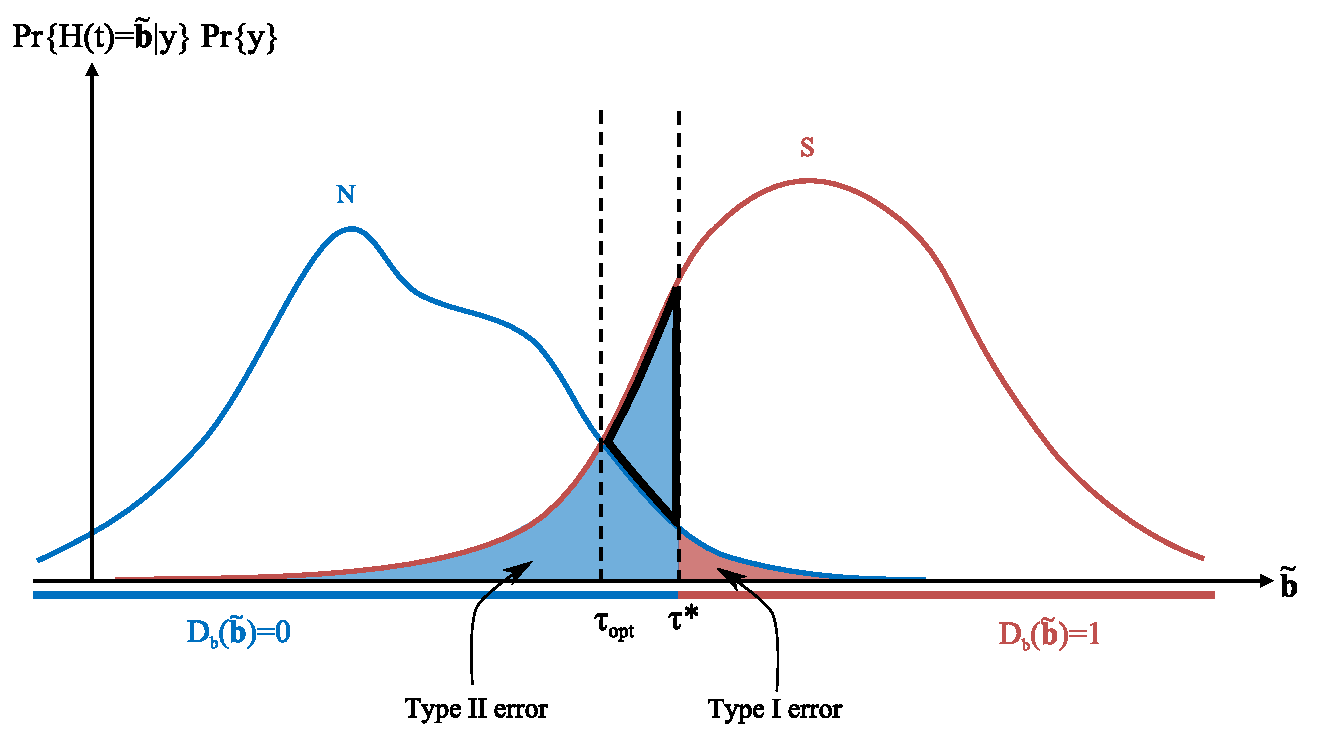
\includegraphics[width=0.9\textwidth]{chap_DET/error}
\caption{Overlapping distributions $N$ and $S$.}
\label{fig:error}
\end{figure}


\begin{theorem}
For any binary detector $D_b$, the symmetric error is bounded below by
$$
\sum_{t=1}^T \min{(s(\bsig_t) (1-\lambda), n(\bsig_t) \lambda)}.
$$
\end{theorem}
\begin{proof}
The error probability consists of two terms; that is, type I and type II errors as shown in Equation~(\ref{eq:det-error}).
\begin{equation}
\begin{aligned}
		\Prob\{error\} 
		&= \sum_{\substack{t=1 \\ D_b(\bsig)=0}}^T s(\bsig_t) \Prob\{y=1\} + \sum_{\substack{t=1 \\ D_b(\bsig)=1}}^T n(\bsig_t) \Prob\{y=0\} \\
		&= \sum_{\substack{t=1 \\ D_b(\bsig)=0}}^T s(\bsig_t) (1-\lambda) + \sum_{\substack{t=1 \\ D_b(\bsig)=1}}^T n(\bsig_t) \lambda
\end{aligned}
\label{eq:det-error}
\end{equation}
\noindent
As follows from Equation~(\ref{eq:det-error}), it is advantageous to classify a behavior signature $\bsig$ as legitimate if $s(\bsig_t) (1-\lambda) < n(\bsig_t) \lambda$ so that the smaller quantity will contribute to the error sum; the other way around follows analogously. Consequently, the lower error bound as defined in the theorem's statement is achieved.
\end{proof}

Frequently, the type I and type II errors are not considered of equal importance; hence, we can weight them with two constants $\alpha, \beta \in [0,1]$ s.t. $\alpha+\beta=1$. The error probability then follows from Equation~(\ref{eq:det-error-nonsym}). 
\begin{equation}
\begin{aligned}
		\Prob\{error\} 
		&= \alpha \sum_{\substack{t=1 \\ D_b(\bsig)=0}}^T s(\bsig_t) (1-\lambda) + \beta \sum_{\substack{t=1 \\ D_b(\bsig)=1}}^T n(\bsig_t) \lambda
\end{aligned}
\label{eq:det-error-nonsym}
\end{equation}

%A reasonable performance measure is defined as a wighted harmonic mean of 


%
%------------------------------------------------------------------------------------------
%

\subsection{Performance Measures}
\index{detection performance!sensitivity}
\index{detection performance!specificity}
\index{detection performance!precision}
\index{detection performance!F-measure}
Optimality conditions assume that detection is performed with the benefit of perfect information. In practice, knowledge of distributions is not readily available and the detectors are evaluated on a behavior-signature database. 
The common performance measures are:
\begin{itemize}
	\item \emph{sensitivity}, also \emph{true positive rate} or \emph{recall} -- the proportion of deviant signatures, which are correctly identified as such
		\begin{equation}
				\text{sensitivity} = \frac{\text{TP}}{\text{TP}+\text{FN}},% = 1 - \textit{type I error},
		\label{eq:sensitivity}
		\end{equation}
	\item \emph{specificity}, or \emph{true negative rate} -- the proportion of correctly identified legitimate signatures
		\begin{equation}
				\text{specificity} = \frac{\text{TN}}{\text{TN}+\text{FP}},% = 1 - \textit{type II error},
		\label{eq:specificity}
		\end{equation}
	\item \emph{precision}, or \emph{positive predictive value} -- the proportion of correctly raised alarms
		\begin{equation}
				\text{precision} = \frac{\text{TP}}{\text{TP}+\text{FP}}.
		\label{eq:precision}
		\end{equation}
\end{itemize}
In addition, sensitivity and precision, that is, the fraction of detected deviant signatures and the fraction of relevant alarms are ideally close to $100\%$ (that is, no type I and type II errors). \emph{F-measure} considers both the precision and the recall to compute the score as a weighted precision and recall average, where the score reaches its best value at 1 and worst at 0. 
\begin{equation}
	F = 2 \cdot \frac{\text{precision} \cdot \text{recall}}{\text{precision} + \text{recall}}
\label{eq:F-measure}
\end{equation}



%
%------------------------------------------------------------------------------------------
%
\subsection{False Positive Paradox}
%http://en.wikipedia.org/wiki/False_positive_paradox

\index{false positive paradox}
The false positive paradox~\citep{Rheinfurth1998} occurs when the behavior signature-database has a low deviant behavior signature share and the detector's hit rate is lower than the false positive rate. In this case, the false positive test is more probable than the true positive test.

Consider the following example:  suppose a detector $D$ has false alarm rate $0.04\%$ and false negative rate (miss) $0\%$; that is, it marks all deviant signatures.  Now suppose we have a behavior signature database $\mathcal{B}_A$ with a million signatures in which $2$ of $100$ signatures are deviant; that is, $2\%$. The detection scores are as follows:
\begin{equation*}
\begin{aligned}
\text{TP} &= 1,000,000 * 0.02 * 1.0 = 20,000 \text{ signatures (hits)},\\
\text{FP} &= 1,000,000 * 0.98 * 0.0004 = 392 \text{ signatures (false alarms)}.
\end{aligned}
\label{eq:paradox-example1}
\end{equation*}
Hence, a signature is classified as deviant with over $98\%$ confidence; that is, $precision=20,000/20,392$.

Now suppose the same detection is applied to a behavior signature database $\mathcal{B}_B$ in which $1$ of $10,000$ signatures are deviant; that is, $0.01\%$. The detector in this case scores as follows:
\begin{equation*}
\begin{aligned}
\text{TP} &= 100,000 * 0.0001 * 1.0 = 100 \text{ signatures (hits)},\\
\text{FP} &= 100,000 * 0.9999 * 0.0004 \approx 400 \text{ signatures (false alarms)}.
\end{aligned}
\label{eq:paradox-example1}
\end{equation*}
A signature is now classified as deviant with only $20\%$ confidence, since only $100$ of total $500$ signatures marked as deviant are indeed deviant. Given the results on database $\mathcal{B}_A$, it is considered paradoxical that deviant detection is mostly a false alarm in database $\mathcal{B}_B$. The probability of a deviant detection result is hence determined not only by the accuracy of the detection, but also by the distribution of the sampled behavior signatures. Hence it is crucial that historical behavior signature distribution matches the behavior signature distribution on which the detector is applied.



%
%==========================================================================================
%
\section{Detectors}
\index{detector}
\cite{Helman1993} divided detectors into: \emph{modeling approaches}, which require estimation of distributions $s(\bsig)$ and $n(\bsig)$ to directly attack the problem of deviant behavior detection, for example, neural networks~\citep{Biermann2001}, k-nearest neighbors \citep{Govindarajan2009}, na\"ive-Bayes estimators \citep{Kruegel2003}; and \emph{non-modeling approaches} that do not explicitly estimate $s(\bsig)$ or $n(\bsig)$, but use various heuristics to flag deviant behavior patterns, for example, expert rules~\citep{Esponda2004}, plan recognition~\citep{Avrahami-Zilberbrand2007}, and decision trees~\citep{Ektefa2010}.

%Approaches for estimating $r(\bsig)$ include neural networks, k-nearest neighbors, na\"ive-Bayes estimators, 

%
%==========================================================================================
%
\subsection{Frequentist Estimator}
\index{frequentist estimator}
Frequentist estimator is a basic approach that estimates distributions $n(\bsig)$ or $s(\bsig)$. The distribution $n(\bsig)$ is estimated from a historical database of behavior signatures $\mathcal{B}$:
\begin{equation}
		\bar{n}(\bsig) = \Prob\{\bsig\} = \frac{\eta(\bsig) }{|\mathcal{B}|},
\label{eq:freq-n}
\end{equation}
\noindent
where $\eta(\bsig)$ counts the number of the occurrences of the signature $\bsig$ in $\mathcal{B}$.

Two promising models for estimating distribution $s(\bsig)$ are \emph{uniform} and \emph{independence} model.
The uniform model assumes that all signatures are equally likely, regardless of the historical database:
\begin{equation}
		\bar{s}_u(\bsig) = \frac{1}{|\bsig|}.
\label{eq:freq-n}
\end{equation}
\noindent
The \emph{independence} model assumes that the features in the behavior signature $\bsig=\langle f_1, ..., f_L \rangle$ are independent, that is:
\begin{equation}
		\bar{s}_i(\bsig) = \Prob\{f_1, \dots, f_L\} = \prod_{i=1}^{L}{\Prob\{f_i\}}  = \prod_{i=1}^{L}\frac{\eta(f_i)}{|\mathcal{B}|}.
\label{eq:freq-n}
\end{equation}

The models are best illustrated by means of example. Consider a behavior signature structure from the previous example. Suppose further that the historical database consists of $100$ signatures, yielding observed frequencies of the four possible behavior signatures as shown in Table~\ref{tab:freq-example}.
\begin{table}[!ht]
\centering
\caption{Example: Observed frequencies of four possible behavior signatures.}
\renewcommand{\arraystretch}{1.2}
\begin{tabular}{ccc}
	\toprule
	Activity / Landmark		& Kitchen	& Bedroom	\\
	\hline
				Standing	& 3 		& 8			\\
				Lying		& 7 		& 82			\\
	\toprule
\end{tabular}
\label{tab:freq-example}
\end{table}

The frequentist estimator gives us, for example, $\bar{n}(\tuple{kitchen, standing})=0.030$ and $\bar{n}(\tuple{kitchen, lying})=0.070$. With the uniform model, we obtain $\bar{s}_u(\bsig)=0.25$ for any $\bsig$, which gives us ratios $\bar{r}_u(\tuple{kitchen, standing})=8.333$ and $\bar{r}_u(\tuple{kitchen, lying})=3.571$. The uniform model simply exposes signatures less likely to be generated by process $N$, without any reference to process $S$. Hence, the signature $\tuple{kitchen, standing}$ is considered as anomalous, as it is the least frequent in the historical database. 

The independence model gives us $\bar{s}_i(\tuple{kitchen, standing})=0.011$ and $\bar{s}_i(\tuple{kitchen, lying})=0.089$, leading us to ratios $\bar{r}_i(\tuple{kitchen, standing})=0.367$ and $\bar{r}_i(\tuple{kitchen, lying})=1.271$. In this case, the signature $\tuple{kitchen, lying}$ is marked as suspicious because activity \emph{lying} is something relatively unusual to be performed at landmark \emph{kitchen}.


Each of the models is clearly better than the other for certain tasks. While we believe those basic models to be reasonable starting points, we envision a framework in which several models are combined to yield the final evaluation.

%
%==========================================================================================
%
\subsection{Density Estimator}

 The estimation can be based on a distance measure to deviant and legitimate behavior signatures in the historical database $\mathcal{B}$. Suppose the historical database $\mathcal{B}$ can be split into legitimate $\mathcal{B}_n$ and deviant $\mathcal{B}_s$ signatures. The ratio $r(\bsig)$ can be then defined as a ratio between distance to the $k$-nearest legitimate and deviant signatures:
\begin{equation}
		r(\bsig) = \frac{\sum_{\bsig_i \in nn(\bsig, \mathcal{B}_s)}^k d(\bsig, \bsig_i)}{\sum_{\bsig_i \in nn(\bsig, \mathcal{B}_n)}^k d(\bsig, \bsig_i)},
\label{eq:density-r}
\end{equation}
\noindent
where $d$ is a distance measure (for example, Manhattan, Euclidean, or Mahalanobis distance) and $nn$ is a set of signatures ordered by the distance to behavior signature $\bsig$:
\begin{equation}
		nn(\bsig, \mathcal{B})=\{\bsig_1, \bsig_2, \cdots, \bsig_{|\mathcal{B}|}| d(\bsig, \bsig_i) \leq d(\bsig, \bsig_{i+1})\}.
\label{eq:density-nn}
\end{equation}

Practical applications are frequently faced with absence of one of the $\mathcal{B}_n$ or $\mathcal{B}_s$ databases. In this case, the detection is focused on one of the tasks: \emph{suspicious} or \emph{anomalous} behavior detection \citep{Avrahami-Zilberbrand2009}.

 %(\cite{Avrahami-Zilberbrand2009}), where the preceding assumption is that a set of historical behavior patterns $\mathcal{B}$ is already available.
%In other words, deviant behavior is a pattern in the data that either does not conform to the expected behavior (anomalous behavior) or matches previously defined unwanted behavior (suspicious behavior). Deviant behavior patterns are also referred to as outliers, exceptions, peculiarities, surprise, misuse, etc. 

\index{behavior!suspicious behavior}
\begin{definition}
	Consider a set of behavior patterns $\mathcal{B}_s$ that encodes negative (suspicious) behavior. A behavior pattern $\mathbf{b} \not \in \mathcal{B}_s$ is \emph{suspicious} iff
	$$
	\exists \mathbf{b}_i \in \mathcal{B}_s: d(\mathbf{b}, \mathbf{b_i}) < \epsilon.
	$$
\end{definition}
\noindent
In other words, a behavior pattern is considered suspicious if it matches at least one suspicious behavior pattern. 
Since suspicious behavior is usually rare, this approach requires an expert that specifies all the suspicious patterns. Thus, such detection systems can only discover threats that are known {\it a priori}. 
Examples include models that encode possible attacks in intrusion detection systems~\citep{Biermann2001}, trying to identify if an attack is under progress; and models with fall-dynamic templates in remote eldercare systems~\citep{Lee04daily} that are compared to observation to infer whether the situation matches one or more templates.


\index{behavior!anomalous behavior}
The other approach uses a set of behavior patterns in an inverse fashion.
\begin{definition}
	Consider a set of behavior patterns $\mathcal{B}_n$ that encode positive (normal) behavior. A behavior pattern $\mathbf{b} \not \in \mathcal{B}_n$ is \emph{anomalous} iff
	$$
	\forall \mathbf{b}_i \in \mathcal{B}_n:  d(\mathbf{b}, \mathbf{b_i}) > \epsilon'.
	$$
	%where $\Phi(\mathbf{b}, k)$ is a set of $k$ patterns $\mathbf{b}_i$ ordered by the distance to $\mathbf{b}$ ($k$-nearest patterns).
	%$$
	%\Phi(\mathbf{b}, k) = \{b_j| d(\mathbf{b}_j, \mathbf{b}) < d(\mathbf{b}_{j+1}, \mathbf{b}), 1 \leq j \leq k \leq |\mathcal{B}_p|\}.
	%$$
\end{definition}
\noindent
The set of behavior patterns is limited to covering only positive, expected behavior patterns. If a behavior pattern cannot be matched against those patterns, it is announced as anomalous. An advantage of this approach is that it requires only examples of positive behavior, which are usually abundant and attainable. This approach can thus detect unforeseen threats and contingencies. However, one potential issue is false positives caused by an incomplete legitimate behavior set; that is, a legitimate behavior pattern is marked as anomalous if it was not previously included in the set $\mathcal{B}_n$. 
%Examples of anomalous behavior detection include models of legitimate person activities... 


\index{local outlier factor, LOF}
A notable approach is Local Outlier Factor (LOF)~\citep{Breunig00lof}, an outlier-detection algorithm based on computing the local neighborhoods densities. The main idea of the LOF algorithm is to assign to each signature a degree of being an outlier. This degree is the LOF of a vector. Vectors with a high LOF have local densities smaller than their neighborhood and typically represent stronger outliers, unlike vectors belonging to uniform clusters that usually tend to have lower LOF values. 
Due to the local approach, LOF is able to identify outliers in a data set that would not be outliers in another area of the same data set. For example, a point at a small distance to a very dense cluster is an outlier, while a point within a sparse cluster might exhibit similar distances to its neighbors.
%The main advantages of the LOF algorithm are that: (i) it detects outliers with respect to local density, not global model; and (ii) it is able to detect outliers regadless of the data distribution (since it does not make any assumptions about distribution). 

%Assume that $A$ is a set of daily-behavior traces $A={B_1, B_2, ..., B_n}$. To detect an anomalous behavior trace we apply the procedure described in Algorithm~\ref{alg:LOF}. First, for each behavioral trace $B_i$ compute the spatio-activity matrix $M_i$ using Algorithm~\ref{alg:SA_matrix}, then compute the vector $p_i$ of the principal components (Equation~\ref{eq:PCA-1}-\ref{eq:PCA-4}), and add vector $p_i$ to the new dataset $A'$. Next, for each vector $p_i$ compute the $k\_dist_i$ as the distance to the $k^{th}$ nearest neighbor of $p_i$,  compute the reachability distance for each vector $p_i$ with respect to the vector $p_j$, where $d(p_i,p_j)$ is the Euclidean distance from $p_i$ to $p_j$, and compute the local reachability density $lrd_i$ of the vector $p_i$ as the inverse of the average reachability distance based on the $k$ nearest neighbors of the vector $p_i$. Finally, compute the $LOF_i$ of the vector $p_i$ as the ratio of the average local reachability density of $p_i$'s  $k$ nearest neighbors and the local reachability density of the vector $p_i$.


% \begin{algorithm}
% \caption{Anomaly detection.}
% \label{alg:LOF}
% \begin{algorithmic}
% \REQUIRE set of behavior traces $A={B_1, B_2, ..., B_n}$, number of $k$ nearest neighbors
% \ENSURE outlier degree for each behavior trace $LOF_i$
% \STATE $A' \gets \{\}$
% \FOR {$B_i \in A$}
% 	\STATE $M_i \gets sa\_matrix(B_i)$
% 	\STATE $p_i \gets PCA(M_i)$
% 	\STATE $A' \gets A' \cup p_i $
% \ENDFOR
% \FOR {$p_i \in A'$}
% 	\STATE $k\_dist_i \gets k\_distance(p_i)$
% 	\FOR{$p_j \in A', p_j \neq p_i$}
% 		\STATE $r\_dist_{i,j} \gets max(d(p_i, p_j), k\_dist_j))$
% 	\ENDFOR
% 	\STATE $lrd_i = {k \over { \sum_{p_j\in kNN(p_i)}{r\_dist_{i, j}}}}$
% 	\STATE $LOF_i \gets { {1 \over k}{{ \sum_{p_j\in kNN(p_i)}{lrd_j}}} \over lrd_i}$
% \ENDFOR
% \end{algorithmic}
% \end{algorithm}

\index{feature extraction}
The more behavior signature features, the more likely each signature is unique, and the less likely that any fixed size historical set represents a substantial mass of all signatures; that is, any density estimator becomes less reliable.

%
%==========================================================================================
%
\subsection{Machine Learning Approaches}

Detectors employ statistical models generated from historical signatures automatically or by an expert. They specify relationships between the values of features and target value. For example, a rule might state if the landmark is \emph{kitchen} and activity is \emph{lying}, then signature is \emph{suspicious}.

If no historical signature is available, an expert specifies a set of rules covering either desired (legitimate) or unwanted (deviant) behavior. Detection is performed analogously as in the previous section.

Data-driven rule generation is defined as a classification task, which constructs a model able to exploit statistical differences in a database of historical behavior signatures. Notable approaches are decision trees, SVMs, neural networks, etc.



%
%==========================================================================================
%
\section{Combining Multiple Detectors}
\label{sec:combine}

As indicated in several studies, it is often advantageous to combine decisions of several experts to reach the final conclusion~\citep{Woods1996, Gams2011principle, Vilalta02}. A single detector might be weak in certain aspect; that is, unable to reliably detect or evaluate specific behaviors. 
For example, consider the ambient assisted living domain. An anomalous event, such as fall, must be detected within seconds, while gradual degradation of gait resulting in limping might require months to be manifested. A detector specialized for anomalous events on the \textit{seconds} scale would be unable to detect such degradation; analogously, a detector  operating on \textit{months} scale would simply filter out events such as falls. The combination of both would address both behaviors to provide anomalous events detection.

The main idea is to construct several local views; that is, detectors trained on a subset of complete feature space such as modalities differences, time scales,  contextual information, and detection method approaches, into the final evaluation.


There are several possible strategies for performing the final evaluation: first, all detectors are considered equally important/reliable; second, accept the decision delivered by the most reliable expert ignoring majority consensus; third, weight detectors by their importance/past perfomance/reliability. A promising direction is to utilize expert knowledge to encode the last approach in a form of a Bayesian network as a set of random variables and their conditional dependencies via a directed, acyclic graph. For example, a Bayesian network could represent the probabilistic relationships between the behavior in question and detectors. Given detectors' evaluations, the network can be used to compute the probabilities that the behavior deviates.


\section{Summary and Discussion}
This chapter helped to understand the anomalous and suspicious behavior detection problem, and why it is difficult to solve. The chapter gave the first clear problem definition and established a theoretical framework for anomalous and suspicious behavior detection from agent traces. We showed how to optimally perform detection, discussed why detection error is often inevitable, and proved the lower error bound. We further provided several heuristic approaches that either estimated distributions required to perform detection or directly rank the behavior signatures using machine-learning approaches.

The main assumption of this chapter was that the decision must is based on a single agent observation. In practice, however, there are often many observations available, which allows the observer to make a decision based on multiple observations. The next chapter extends the theoretical framework to address multiple observations, discusses emerged issues, and proposes an approach to evaluate multiple observations.



%that specifies releationship

%TODO: allow several local views - detectors trained on a subset of complete feature space, they can be weak

%TODO: two possible strategies: all experts are considered equally reliable/important OR accept the decision delivered by the most reliable expert ignoring majority consensus.

% Each human tends to perform activities in a specific way, be it on the micro or macro scale. However, the behavior of the persons in our system is actually monitored from three different points of view. In the first of these, denoted as the \textit{micro level}, one typically deals with behavior that changes in tenths of a second or seconds. For example, one person always carries his identity card in a wallet and puts the whole wallet near the wireless identity-card reader, while another person carries her card in a handbag and requires some time to take it out, identify herself, and put the card back. The person's movement around the access point depends on his/her habits and mental/physical state. These facts determine the persons' patterns at the micro level.

% The second viewpoint, denoted as the \textit{macro level}, describes the persons' daily routines. The activities of interest are the arrival times at access points, the movements between various access points in the access-control network, and even the connections between persons, for example, person $A$ often enters a short time after person $B$. The time scale used at the macro level can vary from seconds to months.

% The third viewpoint, denoted as the \textit{visual level}, captures the persons' visual movement at an access point using a camera. It is also focused on micro-level movements; that is, behavior that changes over a short time interval, but in addition to micro-level features, it obtains features from the visual characteristics of the person and his/her movement, for example, the person's height and the door-opening dynamics.

% Several rules additionally control the regular entry procedure, the regular working time, and the access permissions.


%\section{Time Scales}
%\section{Modalities}

%\subsection{A Bayesian Network Model}

% After the expert rules, micro, macro, visual and meta-learning have made their assessments, their results are integrated into a joint risk analysis of the current entry. It estimates the probability of the event $E = $ \textit{entry is regular} given the observations of the modules. If the estimated probability does not exceed a threshold value, an alarm is triggered. Note that an alarm can also be triggered by expert rules when there is sufficient certainty (type 1 rules).

% The reasoning in the prototype system is performed with a Bayesian network, structured as shown in Figure~\ref{fig:bayesianNetwork}. Four modules have a direct impact on the event $E$; that is, expert rules, micro learning and visual learning, and a macro meta-learning module, while the macro meta-learning module depends only on the three macro modules. The probabilities in the network are computed from the test data, using the \textit{m-estimate}  for conditional probabilities and the \textit{Laplace estimate} for a-priori probabilities. 
% \begin{figure}[h]
% \centering
% \includegraphics[bb=0 540 440 800,width=8cm]{eswa/BayesNetwork2}
% %\includegraphics[bb=30 590 360 820,width=8cm]{img/BayesNetwork.pdf}
% %\includegraphics[bb=0 540 440 800,width=8cm]{img/BayesNetwork2.pdf}
% \caption{Bayesian network used for the reasoning.}
% \label{fig:bayesianNetwork}
% \end{figure}

% The integration proceeds in three steps. Firstly, the output from each module is converted to interval the $[0, 1]$ representing the a-posterior probability $p_{M_i}$ that the entry is regular. Secondly, given the Bayesian network $N$ and the probabilities $p_{M_i}$, the estimated  probability of an event $E$ is computed from the network.
% %\begin{eqnarray}
% %P(E | M_1, M_2, \dots, M_n) = P(E) \frac{P(M_1, M_2, \dots, M_n | E)}{P(M_1, M_2, \dots, M_n)}
% %\end{eqnarray}
% %Numerator is developed with chain rule and due to the structure of the network is simplified to:
% %\begin{multline}
% %P(M_1, M_2, \dots, M_n | E) = \prod_{i=1}^{n} P(M_i | Parents(M_i)) = \\
% % = \prod_{i=1}^{n} p_{M_i} P(M_i=1|E) + (1-p_{M_i}) P(M_i=0|E)
% %\end{multline}
% %Denominator, on the other hand, is independent of the event E, thus is developed as follows:
% %\begin{multline}
% %P(M_1, M_2, \dots, M_n) = \\
% % = \sum_{e\in\{0, 1\}} P(E=e) P(M_1, M_2, \dots, M_n | E=e)  =\\
% % = \sum_{e\in\{0, 1\}} P(E=e) \prod_{i=1}^{n} (p_{M_i} P(M_i=1|E=e) + \\
% % + (1-p_{M_i}) P(M_i=0|E=e))
% %\end{multline}

% Finally, the integration module outputs the joint analysis as a probability that the entry is regular and provides an explanation. According to the threshold values, the integration module triggers \textit{alarm} or \textit{OK} and stores the results in the ontology. In high-security areas, the cost of a false alarm is negligible compared to the cost of an unrecognized intruder; therefore, the system is set to minimize the latter.


\newpage \thispagestyle{empty}

%%!TEX root = thesis.tex





%
%==========================================================================================
%
\chapter{Combining Time Scales and Modalities}
\label{chap:combine}

Each human tends to perform activities in a specific way, be it on the micro or macro scale. However, the behavior of the persons in our system is actually monitored from three different points of view. In the first of these, denoted as the \textit{micro level}, one typically deals with behavior that changes in tenths of a second or seconds. For example, one person always carries his identity card in a wallet and puts the whole wallet near the wireless identity-card reader, while another person carries her card in a handbag and requires some time to take it out, identify herself, and put the card back. The person's movement around the access point depends on his/her habits and mental/physical state. These facts determine the persons' patterns at the micro level.

The second viewpoint, denoted as the \textit{macro level}, describes the persons' daily routines. The activities of interest are the arrival times at access points, the movements between various access points in the access-control network, and even the connections between persons, for example, person $A$ often enters a short time after person $B$. The time scale used at the macro level can vary from seconds to months.

The third viewpoint, denoted as the \textit{visual level}, captures the persons' visual movement at an access point using a camera. It is also focused on micro-level movements; that is, behavior that changes over a short time interval, but in addition to micro-level features, it obtains features from the visual characteristics of the person and his/her movement, for example, the person's height and the door-opening dynamics.

Several rules additionally control the regular entry procedure, the regular working time, and the access permissions.


%\section{Time Scales}
%\section{Modalities}

\section{A Bayesian Network Model}

After the expert rules, micro, macro, visual and meta-learning have made their assessments, their results are integrated into a joint risk analysis of the current entry. It estimates the probability of the event $E = $ \textit{entry is regular} given the observations of the modules. If the estimated probability does not exceed a threshold value, an alarm is triggered. Note that an alarm can also be triggered by expert rules when there is sufficient certainty (type 1 rules).

The reasoning in the prototype system is performed with a Bayesian network, structured as shown in Figure~\ref{fig:bayesianNetwork}. Four modules have a direct impact on the event $E$; that is, expert rules, micro learning and visual learning, and a macro meta-learning module, while the macro meta-learning module depends only on the three macro modules. The probabilities in the network are computed from the test data, using the \textit{m-estimate}  for conditional probabilities and the \textit{Laplace estimate} for a-priori probabilities. 
\begin{figure}[h]
\centering
\includegraphics[bb=0 540 440 800,width=8cm]{eswa/BayesNetwork2}
%\includegraphics[bb=30 590 360 820,width=8cm]{img/BayesNetwork.pdf}
%\includegraphics[bb=0 540 440 800,width=8cm]{img/BayesNetwork2.pdf}
\caption{Bayesian network used for the reasoning.}
\label{fig:bayesianNetwork}
\end{figure}

The integration proceeds in three steps. Firstly, the output from each module is converted to interval the $[0, 1]$ representing the a-posterior probability $p_{M_i}$ that the entry is regular. Secondly, given the Bayesian network $N$ and the probabilities $p_{M_i}$, the estimated  probability of an event $E$ is computed from the network.
%\begin{eqnarray}
%P(E | M_1, M_2, \dots, M_n) = P(E) \frac{P(M_1, M_2, \dots, M_n | E)}{P(M_1, M_2, \dots, M_n)}
%\end{eqnarray}
%Numerator is developed with chain rule and due to the structure of the network is simplified to:
%\begin{multline}
%P(M_1, M_2, \dots, M_n | E) = \prod_{i=1}^{n} P(M_i | Parents(M_i)) = \\
% = \prod_{i=1}^{n} p_{M_i} P(M_i=1|E) + (1-p_{M_i}) P(M_i=0|E)
%\end{multline}
%Denominator, on the other hand, is independent of the event E, thus is developed as follows:
%\begin{multline}
%P(M_1, M_2, \dots, M_n) = \\
% = \sum_{e\in\{0, 1\}} P(E=e) P(M_1, M_2, \dots, M_n | E=e)  =\\
% = \sum_{e\in\{0, 1\}} P(E=e) \prod_{i=1}^{n} (p_{M_i} P(M_i=1|E=e) + \\
% + (1-p_{M_i}) P(M_i=0|E=e))
%\end{multline}

Finally, the integration module outputs the joint analysis as a probability that the entry is regular and provides an explanation. According to the threshold values, the integration module triggers \textit{alarm} or \textit{OK} and stores the results in the ontology. In high-security areas, the cost of a false alarm is negligible compared to the cost of an unrecognized intruder; therefore, the system is set to minimize the latter.



%\newpage \thispagestyle{empty}

%!TEX root = thesis.tex

%
%==========================================================================================
%
\chapter{Accumulating Behavior Evaluations Over Time}
\label{chap:accumulation}

Anomalous and suspicious behavior detection becomes more challenging when agents are observed over a longer period of time. In many domains, no single event is sufficient to determine deviant behavior. Instead, multiple evaluations must be combined. This contrasts with previous chapters, which focused on the detection of a single, clearly suspicious event. 

This chapter proposes a two-step detection system, which first detects trigger events in behavior trace, and then combines the evidence to provide a degree of suspicion. The chapter specifies conditions that any reasonable detector should satisfy, analyzes  three detectors, and proposes a novel detector that generalizes a utility-based plan recognition with arbitrary utility functions.
%The results on a simulated airport domain and a dangerous-driver domain show that our new algorithm outperforms other approaches in several settings.



%\section{Definitions and Assumptions}
%\label{sec:definitions}
%\noindent



% %\subsection{Trigger Events}
% %\label{sec:events}
% %\noindent
% Trigger events can be any kind of partial observations we are able to extract from the domain. In the airport domain, one can focus on people exhibiting indications of suspicious behavior, such as taking photos of critical infrastructure, revisiting the same location, evading the area when noticed, standing in customer service but not requesting the service, etc. 
% %We focus on a rather novel descriptor we were unable to find in the literature on suspicious behavior detection at the airport. 
% We focus on a well-known detector obtained from conversations with domain experts. %and commonly used by behavior detections officers\footnote{An approach for monitoring behavior of passengers over longer periods of time relies upon security personnel such as behavior detection officers (BDOs) that patrol airport to identify passengers who display \emph{involuntary physical and physiological actions}. US Transportation Security Administration (www.tsa.gov) trained and deployed BDO officers at 161 US airports.}.
% We observe the interactions between agents at the airport, more precisely, we are interested in how a passenger behaves in the presence of a uniformed authority figure. A person exposed to a high level of stress produces behavior that indicates fear, anxiety, pressure, tension, deception, etc. Hence, it is rational for the suspicious agent to minimize contacts with the authorities. Note, that no single avoidance is enough to raise a flag, but many such events put together cause the person to be treated as suspicious. 

% %This results in a set of partial observations describing interactive behavior of a passenger. The recognition process first extracts all interactions between passengers and authority figures inside a given radius, producing a set of trajectory pairs that are transformed to relative presentation. 

% A trigger-event detection able to identify interactive behavior may rely on coupled hidden Markov models (CHMMs), which are briefly described below. The reader is referred to~\cite{Brand} for details; the CHMMs are not the main contribution of the paper.
% %To differentiate between authority-regular and authority-suspicious interactions we present an approach based on coupled hidden Markov models (CHMM). 
% %
% The observations consist of two action traces, namely the action trace of the agent of interest and the action trace of an authority agent when they are within some predefined radius. The CHMMs are able to model the complex, interactive behavior by two HMM chains, where the hidden states from one chain directly impact on the hidden states from the other chain. Figure~\ref{fig:CHMMs} illustrates the CHMM for a pair of action traces with length $l=3$. The current state $Q_t^A$ of agent $A$ is affected by both its previous state $Q_{t-1}^A$ and previous state $Q_{t-1}^B$ of the agent $B$ (similarly $Q_t^B$ is affected by $Q_{t-1}^B$ and $Q_{t-1}^A$). Each state $Q_i$ also impacts the corresponding observation state $Y_t$. For example, if the authority agent moves toward the suspicious agent, the next state of the latter takes this into account and produces an action for an avoidance maneuver. 
% %The joint distribution for a pair of traces of length $k$ can be obtained by unrolling the network until we have $k$ slices, and them multiplying together all of the conditional probability distributions. 


% \begin{figure}[!ht]
% \centering
% \includegraphics[bb=0 0 595 830, angle=-90, width=0.5\linewidth]{graphs/chmm.pdf}
% \caption{An example of CHMM for a pair of action traces with length $l=3$.}
% \label{fig:CHMMs}
% \end{figure}

% A regular passenger may not turn or do anything different in the presence of authorities, while a suspicious person will (although as described below, an observer may not have perfect observability). Therefore, we create and train two CHMMs: $\hat{N}_I$ models the interactions produced by authorities and regular passengers, while $\hat{S}_I$ models the interactions produced by authorities and suspicious passengers. For a new event (interaction) $x$ we compute the posterior probability that the event is generated with both models yielding $\hat{n}_I(x)=\Prob\{x|\hat{N}\}$ and $\hat{s}_I(x)=\Prob\{x|\hat{S}\}$, respectively. %We also experimented with more complex CHMM structures including other features such as relative speed and distance, but the results were comparable or even worse.


%As a trigger event we also extract all turns in absence of authority when the trajectory curvature exceeds a threshold value. Probabilities that a turn event was generated by suspicious $\hat{n}_T(x)$ or regular passenger $\hat{s}_T(x)$ is acquired with frequentist estimator from the learning set $D_l$.
%
%
%The second architecture (Figure~\ref{fig:CHMM-3}) incorporates additional information in the form of a model of relative speed between two agents. This model directly impacts the states of both agents. The idea behind this architecture is to improve recognition results with an additional information.
%
%Note that for an interaction of length $T$ the architectures presented in Figure~\ref{fig:CHMMs} are unrolled to $T$ slices. %(similar as in Figure~\ref{fig:HMM-4}). 


%\begin{figure}[!ht]
%\centering
%\subfigure[]{
%\includegraphics[width=0.25\linewidth]{CHMM-2}
%\label{fig:CHMM-2}
%}
%\subfigure[]{
%\includegraphics[width=0.25\linewidth]{CHMM-3}
%\label{fig:CHMM-3}
%}
%\caption{CHMM presented as 2-sliced DBN: (a) modeling actions of two agents and (b) modeling both actions and relative speed.}
%\label{fig:CHMMs}
%\end{figure}




%%%%%%%%%%%%%%%%%%%%%%%%%%%%%%%%%%%%%%%%%%%%%%%%%%%%%%%%%%%%%%%%%%%%%%%%%%%%%%%%%%%%%%%%%%%


\section{Problem Statement}
\label{sec:problem}

We target a large class of applications where no single event is sufficient to make a decision about whether or not behavior is suspicious. Instead, we face a sparse set of \emph{trigger events} that identifies interesting parts characterizing the behavior trace. 

\begin{definition}
\index{event!trigger event}
	\emph{Trigger event} $e_t$ is an evaluation of a subsequence in behavior trace $\mathbf{b}$. 
	%(s.t.\  $1 \leq i < j \leq k$)
	It is described by probabilities that the corresponding subsequence is suspicious $s(e)$ and normal $n(e)$.
\end{definition}
\noindent

Instead of constructing a behavior pattern from the complete behavior trace, only interesting subsequences are extracted and denoted as trigger events. Each event is then further analyzed as a behavior pattern and evaluated as described in the previous chapter. Multiple trigger events are combined into an event trace.

\begin{definition}
\index{event!event trace}
	\emph{Event trace} $\evec{k}$ is a totally-ordered sequence of $k$ trigger events $\evec{k}=\{e_1,e_2,...,e_k\}$.
\end{definition}

Examples include a potentially suspicious passenger who appears to turn away in the presence of security personnel, but not blatantly so; hence, no single event is enough to raise suspicion.
The main question we address is how to combine multiple events to decide whether an event trace corresponds to the normal or a suspicious agent behavior. 

%There are four challenges that need to be addressed. 
%First, there is no one significant event or incident that would help us to reach a decision immediately; a series of trigger events allows us to reach a decision. Second, we have no knowledge about the exact plans devised by a suspicious person. Third, trigger events include multiple agent interactions complicating recognition in the presence of noise. Fourth, an event's suspicion degree depends on the agent's past behavior. For example, the third suspicious event is evaluated differently than the first, since the agent's previous behavior indicates a tendency to behave suspiciously. Hence, the simple counting of suspicious trigger events cannot be applied, since it accumulates all the events linearly. Furthermore, most plan-recognition methods, which rely on a plan library, are insufficient, since plans are not known in advance.

We address the suspicious behavior detection problem in two steps, as shown in Figure~\ref{fig:two-step-detection}. The first step analyzes an action trace and the surrounding environment to detect trigger events that characterize its interesting parts. The event trace is then evaluated in second step. If the evaluation exceeds a threshold value or is large relative to other evaluations, the event is considered suspicious.


\begin{figure}[!ht]
\centering
\includegraphics[width=0.6\linewidth, bb=34 10 523 530]{graphs/flowchart.pdf}
\caption{Two-step detection of suspicious behavior: (i) detection of trigger events; and (ii) detection of suspicious behavior.}
\label{fig:two-step-detection}
\end{figure}


%This paper presents a two-step approach to suspicious behavior detection from a sequence of an agent's actions. The first step detects trigger events; that is, interesting parts of the sequence that serve as evidence, and estimates the probability that an event is suspicious. For this task we present an approach using coupled hidden Markov models~\cite{Brand} that are able to model interactive behavior. The second step combines evidence from multiple events in order to determine suspiciousness.

The key contributions of this chapter are in the second step, which is defined as a decision problem: {is the behavior of an agent suspicious given a sequence of trigger events?} First, we formally describe the detection problem and specify the conditions that any reasonable detector should satisfy. Second, we analyze three detectors, namely the na{\"i}ve Bayes detector, the hidden Markov models and the utility-based plan recognition (UPR). These detectors, however, either simplify the problem or evaluate the events linearly. Finally, we present a novel detector that generalizes UPR as Function-UPR (F-UPR): we define utilities as a set of functions over state transitions and observations, and introduce an observation utility function that is especially suitable for suspicious behavior detection, since it is able to evaluate events non-linearly.
%
%The experimental evaluation on a simulated airport domain first compares the three detectors with our proposed approach. The best two approaches are additionally compared on the dangerous-driver domain.




%Our methods are general, but for illustrative purposes we will make use of the airport domain to provide examples. We treat subjects as agents in a multi-agent environment. At this point we assume that we can perfectly observe their actions. 

\section{Detection Scheme}

This section formally analyzes how to evaluate a sequence of trigger events. 
Our methods are general, but we will make use of the airport domain (Chapter~\ref{chap:lax}) to provide examples, where the goal is to detect a suspicious passenger from a surveillance camera network. Even though we will be focused on suspicious behavior detection, the same conclusion can be drawn for anomalous behavior detection. 
%We treat subjects as agents in a multi-agent environment. At this point we assume that we can perfectly observe their actions.  

We leverage the Bayesian intrusion-detection framework \citep{Helman1993} to define the problem. At each time step $t$, we observe an event $e_t$, generated by a hidden stochastic process $H$. Now suppose that $H$ is a mixture of two auxiliary stochastic processes, namely the normal process $N$ and the suspicious process $S$. The random variable $y_t=0$ if $e_t$ is generated by $N$ and $y_t=1$ if $e_t$ is generated by $S$. Since a suspicious passenger always emits a suspicious event (and a normal person a normal event), $y$ for a specific agent does not change over time. In reality, there can be many subprocesses contributing to both $N$ and $S$; that is, many normal persons with different behavior patterns. However, here we assume only a single $N$ and a single $S$ that capture all the variability. 

To this point, we assumed that an observer is able to perfectly observe whether an event is generated by $S$ or $N$. In practice, however, it may appear that a normal person emits suspicious events (or vice-versa). An observer might be limited for various reasons, such as an inability to detect characterizing features and noisy trigger-event detectors. Therefore, we relax this assumption as follows. An event $e_t$ is observed as generated by $N$ with the probability 
\begin{equation}
	n(e_t) = \Prob\{H(t)=e_t|y_t=0\}
\end{equation}
and as generated by $S$ with the probability 
\begin{equation}
	s(e_t) = \Prob\{H(t)=e_t|y_t=1\}= 1 - n(e_t).
\end{equation}
The mixture distribution of an event $e_t$ and a prior probability $\lambda$ is
\begin{equation}
  \Prob\{H(t)=e_t\} = \lambda s(e_t) + (1-\lambda) n(e_t).
\end{equation}
  

The objective of suspicious behavior detection is to identify those traces $\evec{k}=(e_1,e_2,...,e_k)$ that are likely to be suspicious activities; that is, traces $\mathbf{x}$ for which
\begin{equation}
		%\Prob\{y_t=1|H(t)=e_t, t=1,...,k\} > \tau,
		\Prob\{y=1|H(t)=e_t, t=1,...,k\} > \tau,
\label{eq:detect-sequence}
\end{equation}
is above some threshold $\tau$ or is large relative to the probability for other traces.
%
%An event $e_t$ may depend on the current step $t$ as well as on the pattern of events generated at time steps prior $t$. 
%This allows that $H$ is non-stationary, where its distribution depends both on actual time step $t$ and previously observed events, for example, if the observer identifies three out of four events in an event trace as generated by $N$, a new event will be most likely again observed as generated by $N$. 
%The non-stationary nature might reflect that: (i) agent behavior depends on his/her prior actions; (ii) agent's executing goals change over time; (iii) behavior changes over time (different population of agents); and (iv) the environment changes over time.

The reason this problem is difficult is the non-linear effect. Consider the following example: suppose we observe a person do a U-turn in front of a police officer, so such that the likelihood that this was a suspicious person becomes high. Later, we see the same person doing a half-turn in front of a police officer. This trigger event, if seen on its own, would not contribute much to the overall suspicion. However, following the initial observed turn, this new turn is a much stronger evidence to be attributed to the overall suspicion, because we bias the new event with our previous observation.

Theoretically, it might be possible to optimally detect suspicious behavior using Equation~(\ref{eq:detect-sequence}). Unfortunately, this is usually not the case in practice. 
%
%TODO: why is this difficult? Why not use existing methods?
%
To see this, let us assume a prior probability $\lambda=\Prob\{y_t=1, t=1, ..., k\}$. In most cases, $\lambda$ is close to $0$, since in real-world applications suspicious activities are rare. 
%
Let the stochastic processes $N$, $S$ and $H$ denote $n(\evec{k})=\Prob\{H(t)=e_t, t=1, ..., k|y=0\}$, ~~$s(\evec{k})=\Prob\{H(t)=e_t, t=1, ..., k|y=1\}$, ~and~~ $h(\evec{k}) = \Prob\{H(t)=e_t, t=1, ..., k\}$, respectively.
Using Bayes theorem we can derive from Equation~(\ref{eq:detect-sequence})
\begin{eqnarray}
\label{eq:bayes}
        \lefteqn {\Prob\{y=1|H(t)=e_t, t=1,...,k\} = \frac{\lambda \cdot s(\evec{k})}{h(\evec{k})} = } \\
		%&&=\frac{\Prob\{y_t=1, t=1, ..., k\} \cdot \Prob\{H(t)=e_t|y_t=1, t=1,...,k\}}{\Prob\{H(t)=e_t|t=1,...,k\}} \nonumber\\
		%&&=\frac{\lambda \cdot s(\evec{k})}{h(\evec{k})} =\nonumber\\
		&&=\frac{\lambda \cdot \prod_{t=1}^k s(e_t|e_i, _{i=t-1,...,1})}{\lambda \prod_{t=1}^k  s(e_t|e_i, _{i=t-1,...,1}) + (1-\lambda) \prod_{t=1}^k  n(e_t|e_i, _{i=t-1,...,1})}. \nonumber
\end{eqnarray}

To this point, we implicitly assumed that the distributions $\lambda$, $n$, and $s$ are reliably estimatable. The degree to which this assumption is valid depends on our detection capability.
%
%For each trace $tr_j=\{e_1,...,e_n\}, tr_j \in D_l$ we have a corresponding trace $Y_j=\{y_1, ..., y_n\}$ that specifies whether events were generated by normal or suspicious agent, meaning $y_1=y_2=...=y_n$. 
Suppose we have a sufficiently large dataset $\mathcal{D}_l$ of labeled event traces: we can estimate the prior probability $\lambda$  using the relative frequency, presenting the number of traces generated by a suspicious agent divided by the total number of traces (since traces can be of different lengths, the quotient is normalized by the traces' length).
%
%TODO: estimation of $\lambda$, $n()$ and $s()$. Prior probability $\lambda$ can be estimated 
%
Note that in order to compute $\Prob\{H(t)=e_t, t=1,...,k|y=1\}$ we have to evaluate
\begin{eqnarray}
\label{eq:bayes-opt}
	&s(e_1) \cdot s(e_{2}|e_1) \cdot ... \cdot s(e_k|e_{k-1},...,e_1).
\end{eqnarray}
%which presents a a challenge since we need to specify (or estimate) conditional probabilities of an event for all possible combinations of history. 
While some first terms, that is, $s(e_t), s(e_t|e_{t-1})$, can still be estimated, latter term estimation, including increasingly more history, becomes less and less reliable. In real-world applications, we have no direct knowledge of the conditional probabilities values; that is, we are unable to specify the probability of an event given all the possible combinations of history. For this reason, we must approximate the Bayes optimality in general. In particular, we will be concerned with estimating $\Prob\{y=1|H(t)=e_t, t=1,...,k\}$ using approximate approaches.

%Problems ??:\\
% - it is hard to get probabilities for every possible history length\\
% - we need to simplify: limited history (we may lose important information), event independence (but events are not independent)\\
% - also: does not incorporate observer's bias (solution: UPR)\\
% - solution: heuristics -- scoring functions




%\subsection{Well-behaved Scoring Functions}
%\noindent
Given an event trace, some events may appear suspicious and some not. Hence, detection systems must have a scoring function that combines the evidence. Function output is interpreted as the degree of suspicion attributed to the event trace. Although any two scoring functions need not be exactly the same, we can specify the conditions that any reasonable scoring function must satisfy.  The class defined below appears to be both natural and general.

The detection system can employ a \emph{scoring function} $f$ that interprets events to produce a score characterizing the overall suspicion of the trace. Given a threshold value $\tau$ and an event trace $\evec{k}$, we can classify $\evec{k}$ as suspicious if $f(\evec{k}) \geq \tau$.
\begin{definition}
	A scoring function $f$ over a trace of events $\evec{k}$ is a function
	$$
	f: \bigcup_{k=1}^{K} \evec{k} \rightarrow  \mathbb{R}.
	$$
%	$$
%	f: <\{s(e_1), n(e_1), ..., s(e_n), n(e_n)\}>^{2n} \rightarrow  R
%	$$
\end{definition}
The function $f$ assigns a real value to any trace $\evec{k}$ of length $k=1,...,K$. 

\noindent
Let $\Delta(e_t)$ decide whether a single event $e_t$ is suspicious or not given a threshold $\tau'$:
\begin{eqnarray}
\label{eq:delta}
        \Delta(e_t) = 
			\begin{cases}
		   1; & \text{if } {s'}(e_t) \geq {\tau'} \\
		   0; & \text{else }
		  \end{cases},\\
		{s'}(e_t)=\frac{\lambda \cdot {s}(e_t)}{\lambda \cdot {s}(e_t) + (1-\lambda) \cdot {n}(e_t)}.
\end{eqnarray}

\begin{definition}
A class of \emph{well-behaved} functions consist of scoring functions s.t. $\forall \evec{k}, e_{k+1}:$
\begin{eqnarray*}
f( \evec{k}, e_{k+1} ) \geq f(\evec{k}) &&\textrm{ if } \Delta(e_{k+1}) = 1, \\
f( \evec{k}, e_{k+1} ) \leq f(\evec{k}) &&\textrm{ if } \Delta(e_{k+1}) = 0.
\end{eqnarray*}
\end{definition}
\noindent The conditions imply that the scoring function $f$'s evaluation increases when a new suspicious event is added to the trace, and decreases when a normal event is added to the trace. The well-behaved scoring functions are motivated by the key observation that a suspicious event $e_{k+1}$ (that is, $\Delta(e_{k+1})=1$) is more likely to be generated by a suspicious process $S$ than a normal process $N$, regardless of the history $\evec{k}$, that is, 
\begin{eqnarray*}
s(e_{k+1}|\evec{k}) \geq n(e_{k+1}|\evec{k}) &&\textrm{ if } \Delta(e_{k+1})=1 \textrm{ and }\\
s(e_{k+1}|\evec{k}) \leq n(e_{k+1}|\evec{k}) &&\textrm{ if } \Delta(e_{k+1})=0.
\end{eqnarray*}
%Given such assumptions the likelihood that a trace is emitted by a suspicious process as given by Equation (\ref{eq:bayes}) is a well-behaved function. 

\section{Detectors}
\label{sec:acc-detectors}
\index{detector}
%Several approaches have been proposed to tackle the problem of suspicious behavior detection and the literature is vast. Much of it is only superficially related, in the sense that the overall goals may be the same, but the application domains and the applied methods differ. For instance, detecting suspicious behavior from video surveillance cameras pursue the same goal, but the focus is on video analytics \cite{Visontai}. Similarly, we will not address here related work on suspicious behavior detection from video features, for example, \cite{Arsic,Bak2009,Barbara2008} or anomalous trajectory shapes \cite{Nguyen2005,Piciarelli,Sillito2008,Tung2010}. We focus instead on the observable actions of agents that reveal their intentions. We thus limit ourselves to related research within recognition of multiple events giving a special focus to Hidden Markov Models (HMMs)~\cite{Rabiner1989} and Utility-based Plan Recognition (UPR)~\cite{Avrahami-zilberbrand2007}. 
%Geib and Goldman~\cite{Geib2002}, for example, addressed the problem of recognizing the plan abandonment resulting in an explosion of hypothesis, which was solved by probabilistic plan revision. However, the main difference between related work in plan recognition and our approach is that we do not assume any plan library but rather evaluate events.


%TODO: optimal detection is not possible...

%Given any set of rules, a new transaction may pass some rules and fail others. 
\noindent
This section analyzes approaches that determine whether an event trace is suspicious. First, we discuss the na{\"i}ve Bayes detector that relaxes the initial assumptions. Next, we discuss an approach that directly tackles estimating the likelihood that a trace was generated by a suspicious process using HMMs. Finally, we analyze an approach based on plan recognition and present two extensions: (i) we define utilities as a potential function; and (ii) we present an observation utility function able to address non-linear accumulation.

%They estimate conditional probabilities either by simplifying the assumptions or by modeling the conditional probabilities with another process. Finally, as an alternative, we discuss approaches that do not explicitly estimate the probability. Instead, they use heuristics, statistical measures, and plan recognition framework to provide an evaluation that the trace is generated by suspicious agent.

%There are two approaches to detecting deviant behavior~\cite{Avrahami-Zilberbrand2009}: \emph{suspicious} and \emph{anomalous} behavior detection. The first approach assumes a behavior library that encodes \emph{negative behavior}, and thus recognizing observed behavior corresponds to identifying a match in the library. The second approach uses the behavior library in an inverse fashion, meaning that the library encodes only \emph{positive behavior}. When an observed behavior cannot be matched against the library it is considered as anomalous. 




\subsection{Na{\"i}ve Bayes Detector}
%myopic approximation of Bayesian
%The resulting Bellman equations are identical to the above equations for Bayesian planning, except the belief state is not updated on the right-hand side
\noindent
A naive approach assumes that events are independent, 
%(i) events are independent and (ii) processes $\hat{N}$ and $\hat{S}$ are stationary, 
which means that the current event depends only on the current time step $t$ and not on the time steps prior to $t$. The evaluation of Equation~(\ref{eq:bayes}) is simplified using the naive assumption:
\begin{eqnarray}
\label{eq:naive-bayes}
    \lefteqn {\Prob\{y=1|H(t)=e_t, t=1,...,k\} = }\nonumber \\
	&&\frac{\lambda \cdot \prod_{t=1}^{k}\hat{s}(e_t)}{\lambda \cdot \prod_{i=1}^{k}\hat{s}(e_t) + (1-\lambda) \cdot \prod_{i=1}^{k}\hat{n}(e_t)}. 
\end{eqnarray}
We have to evaluate the probability $\Prob\{H(t)=e_t|y_t\}$ that an event is generated by both a normal process $\hat{n}(e_t)$ and a suspicious process $\hat{s}(e_t)$, which is tractable in terms of evaluation. The approaches for estimating $\hat{n}$ and $\hat{s}$ may include a frequentist estimator, hidden Markov models, k-nearest neighbors, neural networks, etc. We showed an approach using CHMM in Section~\ref{sec:ar:interactions}. An evaluation of the event trace is also well behaved when $\tau'=\lambda$.

In practice, the model may be oversimplified by the assumptions; however, we will use it as a baseline in our experiments.


\subsection{Hidden Markov Models}
\noindent
\index{hidden Markov models}
A conditional probabilities estimation including the history can be encoded with HMMs \citep{Rabiner1989}, as described in Section~\ref{sec:ar:hmm}. 
%A HMM is a temporal probabilistic model with two embedded stochastic processes: an unobservable (hidden) process $Q$, which can be observed only through another (visible) stochastic process $O$. Each state in $Q$ has state-transition probabilities (which are visible) and a probability distribution over the possible values of $O$. The key assumption is that the current hidden state of the agent is affected only by its previous state. 
%
Now suppose we create an HMM to estimate $\Prob\{H(t)=e_t|y=1, t=1,...,k\}$; more precisely, it models the probability that an event trace is generated by a suspicious agent. The hidden states of the process $Q$ may be referred to as internal states presenting the suspicious agent's intentions. For the sake of clarity, let us assume only two hidden states: a normal intention and a suspicious intention, emitting normal and suspicious events, respectively. The transitions between the hidden states can be explained as probabilities that the agent will either follow or change its current intention. 
Informally, this intention switching  may be interpreted as follows: from an observer's perspective, sometimes suggesting that the observed agent is switching intentions appears to provide a better explanation of the behaviors.
%Note, that HMM here relaxes assumption that a suspicious agent always emits suspicious events and allows hidden states to emit different events. In general, a HMM can comprise several hidden states blurring the intuition what intentions present.

%HMM also relaxes the assumption that a suspicious agent always emits suspicious events. do not assume that a particular hidden state (that is, intention) 

We construct two HMM models: a normal model $\bar{N}$ and a suspicious model $\bar{S}$. We split all the labeled event traces $\mathbf{e} \in D_l$ to traces generated by normal and suspicious agents, and use them to learn the parameters of the models $\bar{N}$ and $\bar{S}$, respectively. The parameters can be locally optimized using an iterative procedure such as Baum-Welch method \citep{Rabiner1989}.
%
Given a new event trace $\evec{k}=(e_1, e_2, ..., e_k)$, we compute the probability that the trace was generated by each model $\Prob\{\evec{x}|\bar{N}\}$ and $\Prob\{\evec{x}|\bar{S}\}$ using a forward-backward procedure \citep{Rabiner1989}. Given the prior probability $\bar{\lambda}=\Prob\{y_t=1, t=1,...,k\}$, we estimate the trace $\evec{k}$ was generated by the suspicious process $S$:
\begin{eqnarray}
\label{eq:hmms}
    \Prob\{y=1|H(t)=e_t, t=1, ..., k\} = \frac{\bar{\lambda} \cdot \Prob\{\evec{k}|\bar{S}\}}{\bar{\lambda} \cdot \Prob\{\evec{k}|\bar{S}\} + (1-\bar{\lambda}) \cdot \Prob\{\evec{k}|\bar{N}\}}. 
\end{eqnarray}

Although the information about previous behavior is now partially encoded in the transition probabilities (that is, given that the agent's intention at time step $t$ is suspicious, it is more likely that the intention at $t+1$ will be suspicious as well), the model still uses the Markov assumption; that is, the next agent's intention depends only on its current intention. It is possible to introduce more complex HMM structures with long-term dependencies, but learning and inference in such models becomes computationally intractable \citep{KollerFriedman2009}.


%Both of these baselines share the property that their re- ward bonuses decrease independently per state's action pair as each is sampled. Both intuitively measure the uncertainty the agent has for that state–action pair. However, neither accounts for information contained in the prior distribution (unless that prior is a fac- tored Dirichlet). In the next subsection, we define the variance-based reward bonus, which is capable of mea- suring the uncertainty of arbitrary Bayesian priors over environments

%The approaches discussed so far require estimation of the conditional probabilities including all the history. We call them \emph{modeling approaches}. On the plus side, they directly attack the problem of suspicious activity detection, while on the minus side, modeling approached require simplifications that are likely to be sensitive to the amount of data available for learning. As an alternative, we discuss \emph{nonmodeling approaches} that do not explicitly estimate probability. Instead, they use heuristics, statistical measures, and plan recognition framework.

%Todo: use Markov assumption

%Hidden Markov Models (HMMs)~\cite{Rabiner1989} are widely used in traditional activity recognition for representing and learning a sequence of actions. HMM is a temporal probabilistic model with two embedded stochastic processes: an unobservable (hidden) process which can be observed only through another stochastic process that produces the sequence of observations. Each state has state transition probabilities (which are visible) and probability distribution over the possible output symbols. The key assumption is that the current state of an agent is affected only by its previous state.


\subsection{Utility-Based Plan Recognition}
\label{sec:UPR}
\index{utility-based plan recognition!UPR}
\index{plan recognition}
%Todo: utility-based approach, incorporates stationary observer's bias 
\noindent
We exploit UPR, a \textit{Utility-based Plan Recognition}, briefly described below. The reader is referred to~\cite{Avrahami-Zilberbrand2007} for details.
%
UPR consists of a plan library, which encodes observed agent behaviors in a form of directed graph, and a matching algorithm. It follows the footsteps
of the hierarchical HMM in representing probabilistic information in a plan library. 
%Plan step $q$ is a set of actions that maintain or achieve a goal. 
A plan step can be atomic, or non-atomic; that is, broken down into atomic sub-steps, each a plan step in itself. 
%A plan sequence $\langle q_1, q_2, ..., q_n \rangle$ is a totally ordered sequence of 
Plan steps are linked via sequential edges, describing the execution order of a given plan and its sub-steps. 
%For each plan step three probabilities are maintained: sequential transition probability,  interruption probability (of the sequence in current plan step), and decomposition probability (from the current plan step into its substeps).
%Each leaf has an output emission probability vector $B=b(o)$ over observation symbols. Similarly, 
%UPR introduces three types of utilities on the edges: (a) sequential utility $u_{i,j}$ from the current step $q_i$ to $q_{i+1}$; (b) interruption utility $v_{i, end}$ from the current step $q_i$ to the end of the current plan step $q_{end}$; and (c) decomposition utility $w_i^{d}$ from the current step $q_i^d$ at level $d$ to its first substep $q_k^{d+1}$ at the level $d+1$. A corresponding probability is maintained for each utility.
%
UPR introduces three types of utilities on the edges: (i) the sequential utility from the current step to the next; (ii) the interruption utility from the current step to the end of the  plan; and (iii) the decomposition utility from the current step at current level to its first substep at the sub-level. A corresponding probability is maintained for each type of utility.
%
%Input to the UPR is an observation sequence $o$ that in our case corresponds to an event trace $\mathbf{x}$. 
The observation sequence $o$ is matched against the library using a \textit{Symbolic Plan Recognizer} \citep{Avrahami-Zilberbrand2009}, which filters hypotheses that are consistent with $o$. Finally, the hypotheses are ranked by their expected utility.

We use a heuristic version of UPR as follows: let $\hat{s}(e_t)=1-\hat{n}(e_t)$ be the probability that the trigger event $e_t$ was generated by a suspicious person. Let $c_s>0$ be the cost of the damage caused by a suspicious person if we do not stop him, and, similarly, let $d_n=0$ be the cost of the damage caused by a normal person. The expected cost of letting this person go (marking him as normal) is $c_{go} = c_s \hat{s}(e_t)  + d_n \hat{n}(e_t) = c_s \hat{s}(e_t)$. Now suppose $c_n>0$ is the cost of arresting an innocent person and $d_s=0$ is the cost of the damage caused by a suspicious person when arrested. The expected cost of stopping this person (marking him as suspicious) is $c_{stop} =  c_n \hat{n}(e_t) + d_s \hat{s}(e_t) = c_n \hat{n}(e_t) $. 
If there was only one event, we would compare both hypotheses and choose the one with the lowest expected cost. Supposing in this case $c_n \hat{n}(e_t)$ is lower, we would call this person suspicious.

One possible approach, based on the above expected-cost calculation, would be to determine whether to categorize a trigger event as suspicious or normal, and then to accumulate the total number of suspicious events, and subtract the total number of normal events; unfortunately, this simple strategy performs poorly. %Therefore, we add weights, so that not only do we count whether an event is suspicious or normal, but give it a weight, proportional to the benefit or cost accrued. 
Therefore, not only do we count whether an event is suspicious or normal, but we give it a weight proportional to the benefit or cost accrued. 
%
%Following the approach for identifying a dangerous driver~\cite{Avrahami-Zilberbrand2009}, we propose two single-plan steps encoded in the plan library, as shown in Figure~\ref{fig:UPR}. Note that instead of utility we use the notion of cost. \hl{An agent producing an event $e_t$ follows step $q_s$ (suspicious event) with the sequential probability $\hat{s}(e_t)$ or step $q_n$ (normal event) with the sequential probability $\hat{n}(e_t)$, followed by the end of the plan. We assign two costs: (i) $c_n$ for marking a normal person as suspicious; and (ii) $c_s$ for marking a suspicious person as normal. All other costs are zero. At each event a hypothesis with the highest expected cost is selected. 
The function $U_{\UPR}$ then evaluates an event trace $\evec{k}$ of a person by accumulating the weighted benefit of stopping this person and subtracting the weighted cost of arresting a normal person:
\begin{eqnarray}
	U_{\UPR}(\evec{k}) &=&  \sum_{t = 1}^{k} u(e_t),\\
	u(e_t) &=& 
		\begin{cases}
		~~~~c_s \hat{s}(e_t); & \text{if } c_n \hat{n}(e_t) \leq c_s \hat{s}(e_t) \\
	   		-c_n \hat{n}(e_t); & \text{if } c_n \hat{n}(e_t) > c_s \hat{s}(e_t) \\
	  	\end{cases}.
\end{eqnarray}
If the accumulated cost exceeds a threshold value $\tau'$, the person (that is, trace $\evec{k}$) is marked as suspicious.

This remains a heuristic approach and further investigations could be a topic for future work; however, given that our next approach has significantly superior results, we chose to investigate that in more detail rather than providing more heuristics for the current approach.

% 
%\begin{figure}[!ht]
%\centering
%\includegraphics[width=0.6\linewidth]{UPRplan}
%\caption{A single-step plan in the UPR plan library.}
%\label{fig:UPR}
%\end{figure}

%Such a plan avoids the precise modeling of adversary plans, which are not known in advance. Instead, the only inputs are trigger events and the plan recognizer must combine the evidence to produce a score. Although the evaluation function $U_{\UPR}$ is well behaved, the utilities are constant and hence do not allow a dynamic adjustment to the behavior of the agent in the past. Thus, for instance, the first time we note a suspicious event, and the second time we note the same agent making a suspicious event, count equally.

%In this approach the utilities are constant and hence do not allow a dynamic adjustment to the behavior of the agent in the past. Thus, for instance, the first time we note a suspicious event, and the second time we note the same agent making a suspicious event, count equally.



\section{Utilities as Potential Functions}
\index{utility-based plan recognition!F-UPR}
\noindent
Although the evaluation function $U_{\UPR}$ is well behaved, the utilities are constant and hence do not allow a dynamic adjustment for past agent behavior; for instance, the first time we note a suspicious event counts equally, with subsequent suspicious events made by the same agent. 
These utilities, however, are unable to express the empirical observation characteristics. Therefore, we extend the notion of utility and define the utility $U$ as follows.
%First, we simplify the notation by writing $u(q_{i-1}, q_i)$, where $u$ is either a sequential, transition or decomposition utility. 
%Next, we define $f$ also over observation sequence $\mathbf{x}$:
\begin{definition}
The utility function $U$ over a plan step $q_a$, a plan step $q_{b}$, and the entire observation sequence $\evec{t}$ until current time step $t$ is a function
$$
U: \langle q_a, q_{b}, \evec{t} \rangle ^n \rightarrow \mathbb{R}. 
$$
\end{definition}
%
Utility function can be written as
$$
U(q_a, q_{b}, \evec{t}) = \sum_{j=1}^n \lambda_j u_j(q_a, q_{b}, \evec{t}),
$$
where each utility function $u_j$ can be sequential, interruption,  decomposition or any other utility, and $\lambda_j$ are parameters to be defined. 
%
This allows us to introduce a set of auxiliary utility functions $u_j$ describing not only the plan-step transitions but also the additional characteristics of the observation sequence. For example, the sequential utility from step $q_i$ to $q_{i+1}$ can be written as $u_t(q_i, q_{i+1}, \evec{t}) = c$, but in general, the constant $c$ can be replaced with any function over $q_i$, $q_{i+1}$ and $\evec{t}$.


\begin{theorem}
$U$ is a well-behaved function iff $$\forall u_j, j=1...k: u_j \text{ is a well behaved function.}$$
\end{theorem}
\begin{proof}
Consider two well behaved functions $f$ and $g$, and two scalar constants $\lambda_f$ and $\lambda_g$. Let  $f'=\lambda_f f$. Since it is easy to see that multiplication with scalar constants preserves the well-behaved property, $f'$ is also a well behaved function. Let function $u$ denote $u=f'+g'$. Then, $u(\evec{t}, e_{t+1})$ $=$ $f'(\evec{t}, e_{t+1})+g'(\evec{t}, e_{t+1}) \geq u(\evec{t})$ $=$  $f'(\evec{t})+g'(\evec{t})$ ~if $\Delta(e_{t+1}=1)$, since $f$ and $g$ ~are ~well behaved ~and ~therefore $f'(\evec{t}, e_{t+1})$ ~and ~$g'(\evec{t}), e_{t+1})$ ~are ~~non-negative. ~~Similarly, $f'$ and $g'$ are non-positive when $\Delta(e_{t+1})=0$.
\end{proof}




%TODO: what is wrong with this

%\subsection{Scoring Functions}
%TODO: summarize previous approaches, motivate our solution
%All of the previous approaches (except HMMs) share the property that events are evaluated according to the probability of being generated by the suspicious process.
%However, neither fully use the information contained in the prior behavior of the agent -- HMMs consider only the previous state, while UPR considers linear relation between the events.
%In this subsection, we define the scoring function, which is capable of estimating event in a trace according to the complete prior history in a non-linear fashion.




%
%The true likelihood function is difficult to obtain. Therefore, we defined the following well-behaved heuristic function to approximate it.
%
%TODO: introduce rule for $\eta_n(j)$


\subsection{Exponential Observation Utility}
\label{sec:FUPR}
\noindent
In order to include agent past behavior in an evidence evaluation, the utility function must be defined over the observation sequence.  We propose an observation utility function that assigns cost using the number of past normal and suspicious events.
%
Consider the example from Section~\ref{sec:problem}. Suppose we see a person do a full U-turn in front of a police officer and we give this event a cost of 1. Later, we see the same person doing a half-turn in front of a police officer. This event if seen on its own, would be given cost 0.5. However, following this initial turn, this new turn becomes a 1 instead of 0.5. So, a linear accumulation would have given us a cost of 1.5, whereas because we bias the new event to register higher on our scale, our cost is 2 instead of 1.5.


Let $\eta_s(\evec{k})$ define the number of suspicious events in an event trace $\evec{k}$:
\begin{equation}
        \eta_s(\evec{k}) = \sum_{t=1}^k\Delta(e_t).
\end{equation}
%where $\lambda_\eta$ is prior probability for detecting suspicious event (if we have no prior knowledge, we can assume $\lambda_\eta=0.5$), $\hat{s}$ and $\hat{n}$ can be the same procedures as discussed previously, and $\tilde{\tau}$ is a threshold value (if $\lambda_\eta = \tilde{\tau} = 0.5$ the condition in~(\ref{eq:delta}) can be simplified to $\hat{s}(e_t) > \hat{n}(e_t)$).
Similarly, let $\eta_n(\evec{k}) = k - \eta_s(\evec{k})$ represent the number of normal events. 
%
Suppose we observed a trace $\evec{k}$ of all the suspicious events; that is, $\forall t, t=1,...,k: \Delta(e_t) = 1$. Intuitively, %terms in Equation~(\ref{eq:bayes-opt}) suggest that
the likelihood that an event $e_t$ was indeed generated by a suspicious process increases exponentially according to the number of suspicious events in the past. % terms; that is, to the number of events. 
On the other hand, if the events in $\mathbf{e}$ were normal; that is, $\forall t, t=1,...,k: \Delta(e_t) = 0$, the likelihood decreases exponentially as the number of normal events increases.
%TODO: introduce an instance of the family\\
We define an observation utility function $u_o$ over the current event $e_t$ and trace $\evec{t-1}$ recursively as follows:
\begin{eqnarray}
\label{eq:fe}
        u_o(e_t, \evec{t-1}) &=& \psi(\evec{t}) \cdot (u_o(\evec{t-1}) + \omega(\evec{t})),\\
		u_o(\evec{0}) &=& 0,\nonumber\\
		\omega(\evec{t}) &=& \alpha \cdot \eta_s(\evec{t})^{s(e_t) / \beta},\\
		\psi(\evec{t}) &=& \gamma \cdot \rho^{{-\eta^*_n(\evec{t})}/{\eta_s(\evec{t})}}.
		%e^{\frac{\delta \cdot \eta'_n(i)}{(\gamma+\eta_s(i))}} \cdot [f_e(e_{i-1}) + \beta \cdot \eta_s(i)^{\alpha (\tilde{s}(e_i) - \tilde{\tau})}]
			%e^{- \ro \eta_n'(i)/{\gamma + \eta_s(i)}}; & \text{else }
		   	%e^{x}; & \text{else }
\end{eqnarray}
The term $\omega(\evec{t})$ uses an exponential function to assign a cost to the likelihood $s(e_t)$ that an event is suspicious. The parameter $\alpha > 0$ is the initial cost,  $\eta_s$ corresponds to the growth factor, and the parameter $0 < \beta < 1$ is the likelihood of the cost increasing by the growth factor. The parameters $\alpha$ and $\beta$ are estimated from the data. In the case of observing two full U-turns, the second U-turn attributes higher cost to the overall suspicion, since the exponent base is increased due to the first U-turn.

Additionally, the term $\psi(\evec{t})$ employs an exponential time decay function that discounts the accumulated cost at time $t$ according to the number of consecutive normal events $\eta^*_n$. The modified $\eta^*_n$ represents \emph{the time elapsed} since the last  event $\Delta(e_i) = 1$; that is, the number of normal events since the last suspicious event. The higher the number of consecutive normal events, the faster the cost decay. The parameter $0 < \gamma \leq 1$ is the initial decay, the parameter $0 < \rho < 1$ is the decay factor, and $\eta_s$ is used to specify the number of events required for the decay to decrease by the decay factor. The parameters $\gamma$ and $\rho$ are also estimated from the data. Suppose we observe two agents, one already having made two U-turns and the other having made a single U-turn. Suppose, then, we observe both agents do a clearly normal event; the overall suspicion of the first agent is less than the overall suspicion of the second agent. Hence, the higher the number of suspicious events, the slower the suspicion decay.


%Parameter $\beta \geq 0$ is also estimated from the data.  The modified $\eta^*_n$ presents \emph{the time elapsed} since the last event $\Delta(e_i) = 1$, that is, the number of normal events since the last suspicious event; the higher the number of normal events the faster the time decay.}
%Finally, we use a threshold value to decide whether a trace is generated by suspicious agent or not $f_e(\mathbf{x}) > \tau_{f_e}$. 
The function $u_o$ is a well-behaved function by definition. Equation~(\ref{eq:fe}) can be rewritten, which gives us the utility function $U_{\FUPR}$: 
%$$u_o(\evec{k}) =  \sum_{t = 1}^{k}(\omega(\evec{t}) \prod_{i=t}^{k} \psi(\evec{i})),$$ 
%which gives us the utility function $U_{\FUPR}$
\begin{eqnarray}
	U_{\FUPR}(\evec{k}) &=&  \sum_{t = 1}^{k} \sum_{j = 1}^n \lambda_j f_j(\evec{t}, q(t-i), q(t)) \nonumber \\
	%&=& \lambda_d \sum_{t = 1}^{k} d(e_t) + \lambda_o \sum_{t = 1}^{k}(\omega(\evec{t}) \prod_{i=t}^{k} \psi(\evec{i})).\nonumber
	&=& \sum_{t = 1}^{k}(\omega(\evec{t}) \prod_{i=t}^{k} \psi(\evec{i})).
\end{eqnarray}
%\hl{The $U_{\FUPR}$ utility function assigns a cost using both the sequential utility $d(e_t)$ and the observational utility $u_o(\evec{t})$. Their contributions to the accumulated cost are regulated by the parameters $\lambda_d$ and $\lambda_o$. In the practical experiments, however, the observational utility proved to be sufficient, hence $\lambda_d=0$ and $\lambda_o=1$.}

%Consider the following example. Suppose we have a trace $\evec{18}=(e_1, ..., e_{18})$, where events $e_i>\tilde{\tau}$, for $t=\{1,6,12\}$ (most likely suspicious) and $e_t<\tilde{\tau}$ elsewhere (most likely not suspicious). The evaluation of trace $f_e(\evec{k})$ is showed in Figure~\ref{fig:ef-plot} for each time step; that is, after each event. The score is much higher for each subsequent suspicious event, while it decreases at slower rate.
%\begin{figure}[!ht]
%\centering
%\includegraphics[width=0.8\linewidth]{ESPY-example}
%\caption{Evaluation of a trace $f_e(\mathbf{x})$ over time.}
%\label{fig:ef-plot}
%\end{figure}

\section{Summary and Discussion}
This chapter extended the theoretical framework established in the previous chapter. It showed how to perform detection when an agent is observed over longer periods of time and no significant event is sufficient to reach decision. We first specified conditions any reasonable detector should satisfy and analyzed several detectors. We further proposed a novel approach denoted as F-UPR detector that generalizes UPR~\citep{Avrahami-Zilberbrand2007} with arbitrary utility functions. This allows to assign utility to repeated plan steps according to agent past behavior, which was, in turn, used to introduce an exponential observation utility function that assigns cost using the number of agent's past normal and suspicious events.




\newpage \thispagestyle{empty}

%!TEX root = thesis.tex

%
%==========================================================================================
%
\chapter{A Unified Detection Framework}
\label{chap:framework}

In this chapter, a unified framework for anomalous and suspicious behavior detection is presented. The goal is to design a framework rich enough to address various domains and different configurations. Therefore, we summarize its components and explain their relationships. The next part of the thesis then shows how to instantiate the detection framework in various real-life domains.

\section{Framework Components}

\index{unified framework}
All the components presented in the previous chapters form the unified framework for anomalous and suspicious behavior detection. This section reviews the components, their hierarchical structure, and explains the processing steps of the unified framework.

\subsection{Framework Levels}

Let us revisit the framework level hierarchy shown in Figure~\ref{fig:stack} that systematically processes agent spatio-temporal data to perform deviant behavior detection. The information flow is bottom-up through three main levels shown on the left-hand side: measurements, activity assessment, and behavior assessment. Each of the main levels contains several sub-levels (right-hand side): 13 in total. 

The measurement level provides sensor data, which are collected at each time step~$t$ in the next sub-level as an \emph{observation vector} $\mathbf{x}_t$. In addition to the sensor data, the observation vector may also contain contextual information and environmental variables such as time, date, weather, etc. Subsequent observation vectors are bundled in an observation sequence $\mathbf{X}$.

\index{activity recognition pipeline}
The next main level is activity assessment. The first four sub-levels basically correspond to ARPipe (activity recognition pipeline, Chapter~\ref{chap:activity_recognition}), which first suppresses the sensor noise, followed by the construction of activity recognition feature vectors and atomic activity recognition itself. Finally, the spurious transitions among atomic activities that cannot occur in reality are smoothed. \emph{Activity sequence} containing an atomic action at each time step $\avec{T}=\{a_t|1 \leq t \leq T\}$ is passed to the next sub-level, which can recognize complex behaviors or interactions among agents.

The top level performs behavior assessment in order to detect deviance. The first sub-level constructs a \emph{behavior trace} that consists of $\tuple{landmark, activity}$ tuples, which are encoded as a \emph{behavior pattern} in the next sub-level. The next sub-level then introduces a set of detectors based on different features, views and modalities to provide different evaluations of the behavior pattern. The evaluations are then combined at each time step in the next sub-level as well as over time at the level above. Finally, the top sub-level outputs the final agent behavior evaluation that comprehends all the behavior to the current time step. 

%This dissertation designs and implements a general framework for deviant behavior detection that addresses several challenges in physical domains. Within the framework four steps are introduced as shown in Figure 1: (i) activity recognition (yellow box), (ii) behavior signatures (green boxes), which are part of (iii) multi-view evaluation (blue box), and (iv) repetitive behavior detection (orange box). Each step conta


\begin{figure}[!h]
\centering
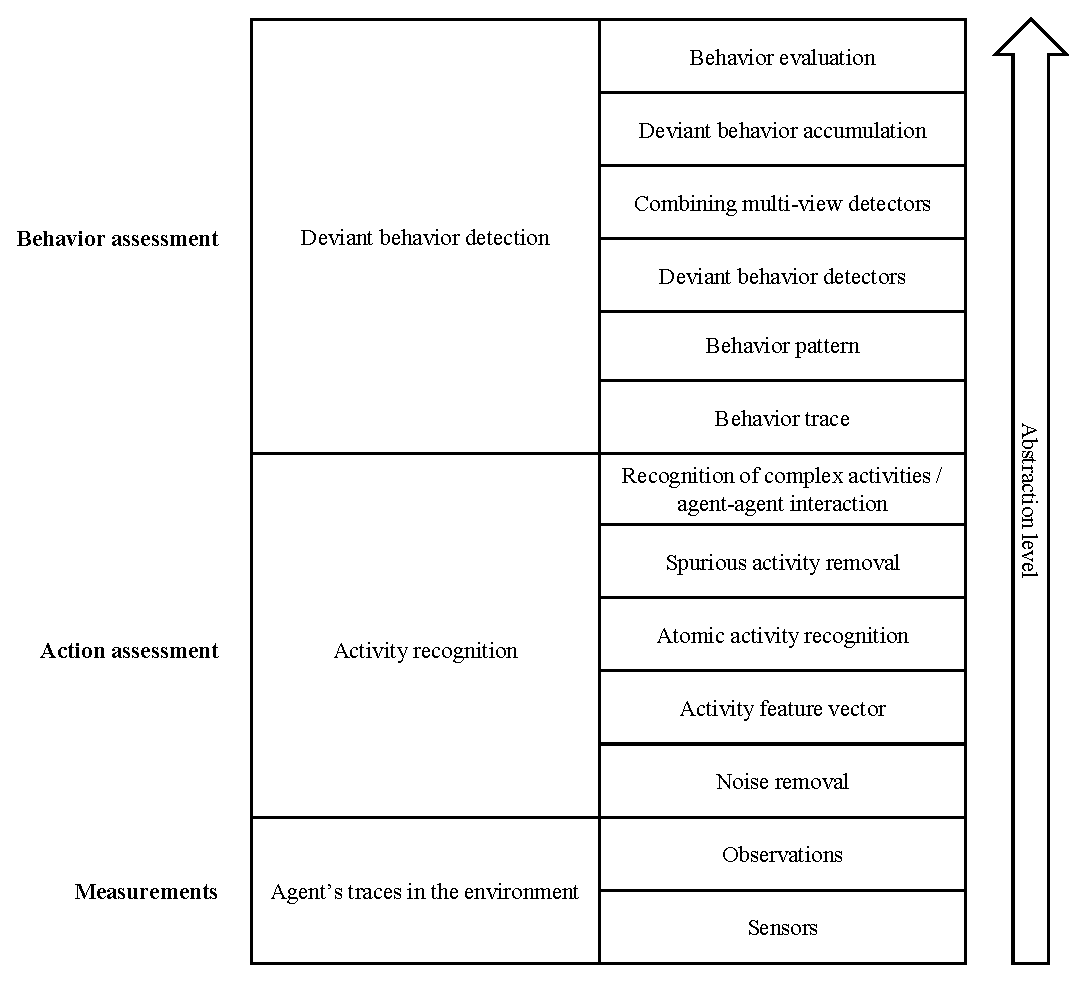
\includegraphics[width=1\textwidth]{chap_FMW/stack}
\caption{Hierarchy of abstraction levels and processes.}
\label{fig:stack}
\end{figure}

\subsection{Processing Steps}

A detailed unified framework flowchart is outlined in Figure~\ref{fig:flowchart}. The start and the end of the process are shown in rounded rectangles, processes are represented as rectangles, and input/output data are represented as a parallelogram.

The process starts with an observation sequence describing agent movements in the environment. The trace is first processed by the activity recognition pipeline as described above and outputs an activity sequence. The activity sequence then enters deviant behavior detection level marked with dashed-squared box. The activity sequence is first augmented to behavior trace, which then enters into a variety of view transformation processes. Each view-transformation process applies its specific viewpoint using either different features, modalities, or time aggregation periods to construct corresponding behavior signatures. Each behavior signature is then evaluated with a deviant behavior detector separately. The next step combines all the evaluations that are further processed in a suspicious behavior accumulation module over time, which finally outputs the input trace deviation.

General implementation principles and the theoretical background of particular flowchart processes were discussed in the previous chapters, while the concreted domain implementation is demonstrated in Part~\ref{part:applications} of this thesis. Note that, in some domains, not all the processes are required; a domain problem may simplify a certain process. For example, if only a single behavior view is required, the multi-view detector combination is simplified accordingly.

\begin{figure}[!h]
\centering
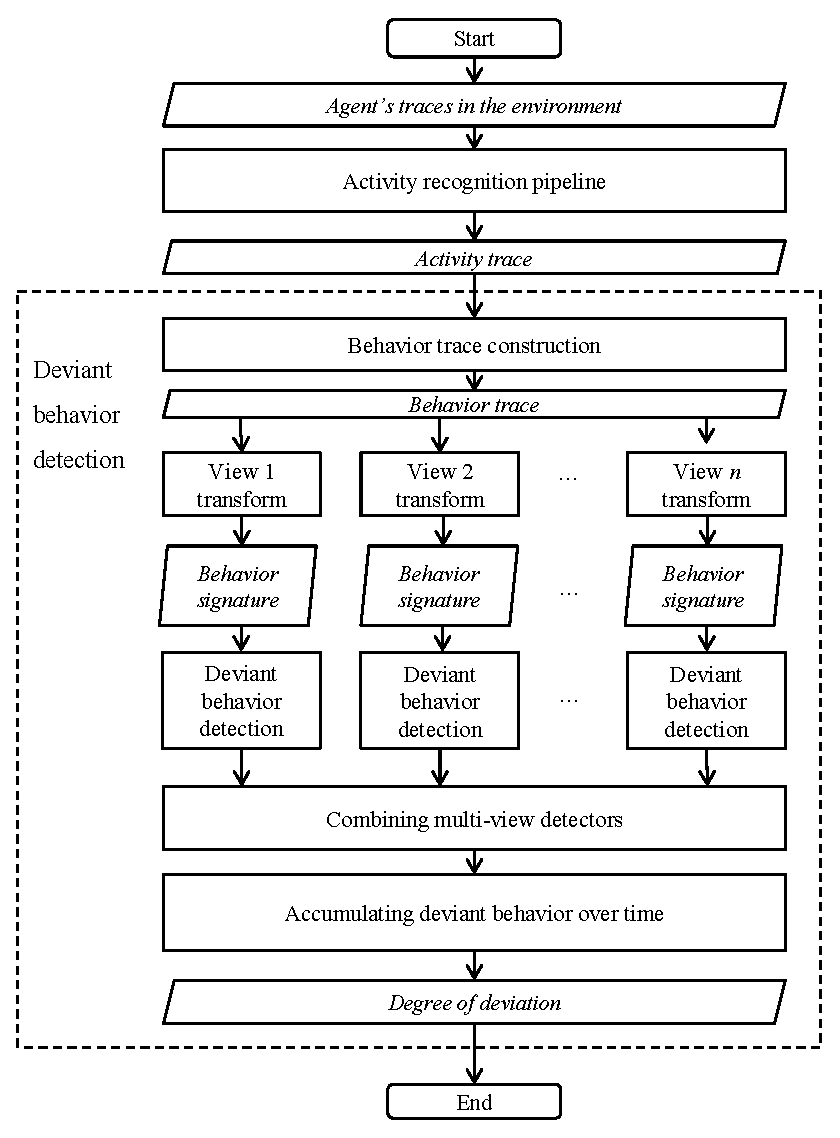
\includegraphics[width=0.8\textwidth]{chap_FMW/flowchart}
\caption{Processing flowchart of the unified framework.}
\label{fig:flowchart}
\end{figure}



\section{Framework Instantiation}
As will be shown in the next part of the thesis, the framework can be instantiated for various domains and problems. 
%The general architecture as shown in Figure~\ref{fig:stack} covers all abstraction hierarchy levels, while specific domains may omit some of the levels due to simplicity or trivial implementation. 
This section covers high-level framework instantiation, emphasizing the learning and detection phases. 

\subsection{Learning and Detection}
Unified framework instantiation includes selecting and designing some
domain-specific components as well as implementing general components described in the previous chapters. Since this will be covered in Part~\ref{part:applications} of this thesis, these components will be abstracted and the focus will be on the learning and detection phase.

Figure~\ref{fig:learning-detection} depicts a high-level block diagram of the learning (left-hand side) and the detection (right-hand side) phase within the unified framework. The goal of the learning phase is to instantiate all the components, which includes building classifiers and detectors, discovering patterns, and fine-tuning the parameters of the models. After that, the framework is deployed in the detection phase, which is dedicated to evaluating new traces at the input.

\begin{figure}[!h]
\centering
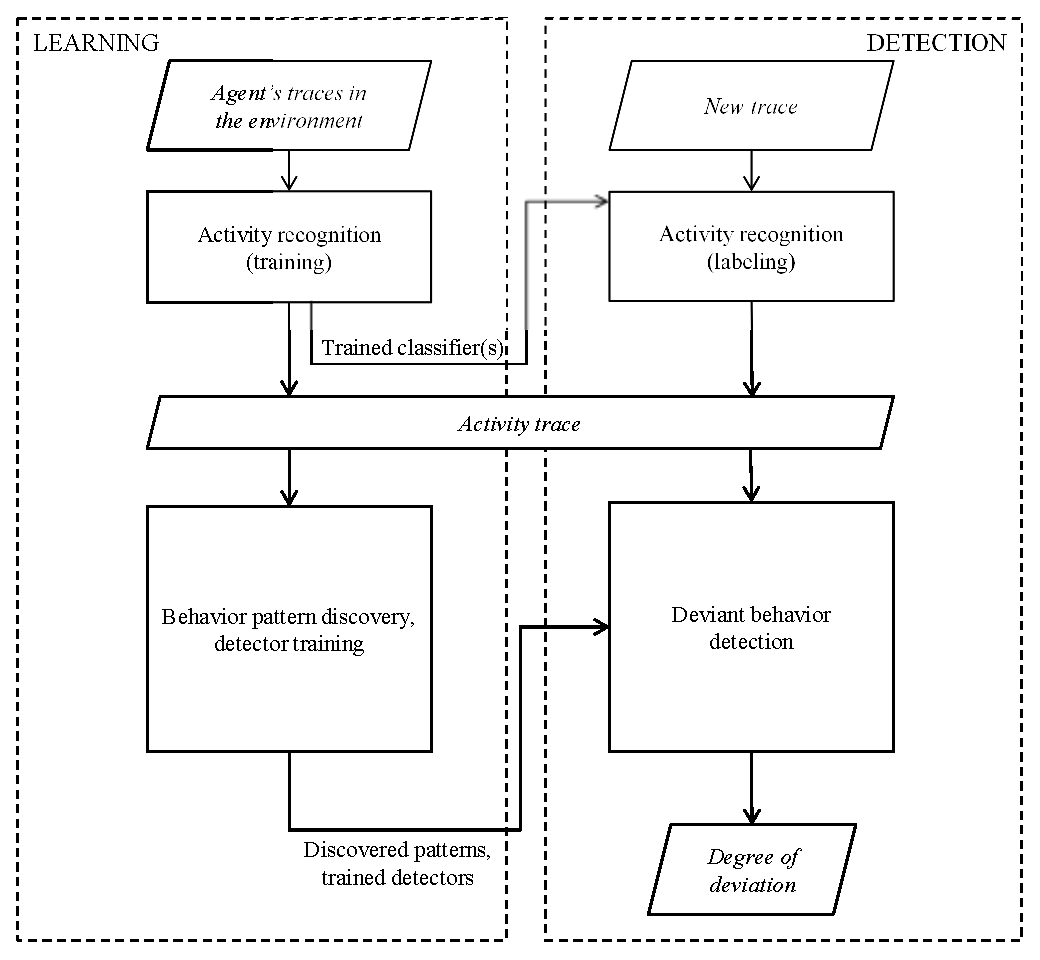
\includegraphics[width=1\textwidth]{chap_FMW/learning-detection}
\caption{Block diagram for learning and detection phases.}
\label{fig:learning-detection}
\end{figure}

The learning phase includes two components that require training. The first component is activity recognition, which, unless the activities are already provided from the environment, requires classifier training. This includes recording labeled training data to construct a training dataset, feature extraction, and building a classification model. Once the model is trained, it can be used in the detection phase. 

%implemented with expert knowledge, ... requires training data ... prerecorded activities .... feature extraction ... model selection ...

The second component is dedicated to behavior patterns construction and detection model training. According to our detection goals, that is, either anomalous or suspicious behavior detection, the aim of this phase is to construct a dataset of positive or negative behavior patterns, respectively, using either automatic/semi-automatic approaches, such as clustering, or domain expert knowledge that encodes behavior patterns. As shown in Figure~\ref{fig:flowchart}, this can be applied for a variety of viewpoints. The next step then includes detector training and initial parameter tuning, which also requires a training dataset.
Note that the second component already requires that the activity recognition component is trained.

\section{Summary}
In summary, we proposed a unified framework for detection of anomalous and suspicious behavior that can be observed from complex, spatio-temporal sequential data generated by an agent moving in a physical environment. The framework incorporates the components introduced in the previous chapters to address the main challenges. The second part of the thesis shows how the framework is instantiated in three empirical studies. 

%For example, behavior evaluation in ambient assisted living domain, where the goal is  some of the levels can be  can be 

%The framework can be applied to 

% \subsection{Framework Evaluation}

% by components...

% "celoten" performance

%\section{Discussion}
%The amount of training data
\newpage \thispagestyle{empty}

%
%==========================================================================================
%
\part{Empirical Studies}
\label{part:applications}

%!TEX root = thesis.tex


%
%==========================================================================================
%
\chapter{Ambient Assisted Living Domain}
\label{chap:confidence}

\index{activities of daily living, ADL}
\index{ambient intelligence, AmI}
\index{daily-living dynamics}
Analyzing  daily-living behavior is an important approach to assessing the wellbeing of an elderly person living at home alone. This chapter presents an approach to monitoring an individual in the home environment by an ambient-intelligence system to detect daily living pattern anomalies. It utilizes the proposed unified framework to recognize activities, extract spatio-activity behavior signatures, and apply an outlier-detection method to classify the individual's daily patterns, regardless of the cause of the problem, be it physical or mental. Experiments indicate that the proposed solution successfully discriminates between healthy person behavior patterns and those of a person with health problems.

\section{Introduction and Background}
\label{sec:introduction}

%
%Set context and motivate the overall field of study 
%
\index{ambient assisted living, AAL}
\index{ambient intelligence, AmI}
Recent years have seen increased interest in the deployment of systems for ambient assisted living (AAL) \citep{Augusto2012}, including remote eldercare \citep{Kaluza2010Agentbased}, smart homes \citep{Cook}, surveillance \citep{Dore}, etc. Whereas some of these systems can be tele-operated, the AAL community strives to design systems that monitor a person autonomously and act in the case of an emergency, warning or suggestion, such as fall detection~\citep{Bourke, Lustrek2009Behavior}. Our study targets persons in the home environment; that is, a male or female senior citizen, who does not need intensive care or assistance in day-to-day living, but accepts an ambient-intelligence (AmI) system to improve their health, safety, and well-being. The main issue is anomaly detection in the monitored person's daily behavior.

%
% Provide a concrete problem statement 
% - person-friendly HW
% - accurate activity recognition
% - uknown activites of DL
% - adaptation to each person
%
A predominant approach consists of three components: a sensor system, an activity-recognition model, and a daily behavior analysis~\citep{Choudhury06towards}. There are several challenges to constructing such a system. First, the person must be monitored with sensors that are not obtrusive, invasive or privacy-violating, yet are precise enough to address the second challenge, which is an accurate activity recognition model. An underlying recognition model needs to detect a wide variety of activities performed differently under different environmental conditions and across many individuals. Third, we have no knowledge about the exact plans and schedules a person may follow during the day. In addition, the system should adapt to each specific person while deployed at the person's home.

%
% Explain why previous work fails in addressing the problem statement 
%
%
% Explain our ideas and why they are new and overcome the limitations of para 3 
%
In remote eldercare, the AAL systems use a wide variety of sensors, such as vision systems~\citep{Fabien}, inertial sensors~\citep{Bourke} and embedded sensors~\citep{Lymberopoulos, Monekosso}. While some sensors might violate privacy issues, for example, a camera, others do not provide additional location context, for example, inertial sensors, or rich information required for accurate activity and posture recognition, for example, embedded sensors. Daily behavior analysis may focus on recognizing or describing exact schedules and assumes that the person will follow them. Another approach relies on either observers, that is, a nurse who periodically observes an elderly person, or on self-reporting, that is, having people complete an activity report at the end of the day. Both ways of reporting have limited accuracy and usefulness due to the aggregation in time, forgetfulness, and misreporting (intentional or unintentional). 

In contrast to related work discussed in Section~\ref{related:behavior:transaction}; that is, fuzzy-association analysis \citep{Lee04daily}, Apriori algorithm combined with Markov chain \citep{Lymberopoulos}, and HMMs \citep{Monekosso}, this chapter uses a localization system (in other publications, accelerometers are more often used) with wireless body-worn tags (described in Section \ref{sec:experiments}), while low-level activity recognition is performed with a SVM classifier. These two modules were developed within the Confidence system \citep{Kaluza2010Agentbased}. This chapter focuses on the third component; that is, daily patterns analysis that detects behavior changes indicating an early discovery of a potential health problem, such as a person visiting a toilet unusually often. In contrast to related work, which mainly dealt with a description of high-level activities, our method focuses on activity dynamics; by contrast to Markov models, it explores the relations between spatial information and activities. %The method detects anomalous behavior regardless of the cause.
The method is general in the sense that it detects unusual behavior regardless of the cause, be it illness of any kind, any physical or mental degradation or even an outside cause, for example, being locked in a room. 

%The central hypothesis is that daily movement patterns can be learned for a specific person and the anomalous behavior can be detected when compared to the learned patterns.
%We propose a presentation that aggregates a daily activity log into a \textit{spatio-activity matrix}. It can be used to visualize the person's daily dynamics. For automatic detection with machine learning we propose a method for evaluating the behavior anomalousness based on principal component analysis (PCA) for feature extraction and the local outlier factor algorithm (LOF)~\cite{Breunig00lof} for detecting anomalous behavior patterns. 


%
% How did you evaluate your new ideas and what were some key results that should motivate the reader to read the rest of the paper
%
%We deployed the system in a lab organized as a near-realistic home apartment of about $25$~$m^2$ and equipped with the Ubisense localization system~\cite{Ubisense}. The activity-recognition model trained on several persons was able to achieve a better than 87\% accuracy in recognizing the activities of a new person~\cite{Kaluza2010Agentbased}. We experimentally tested our new approach in multiple episodes with several persons involving regular behavior and behavior when a person does not feel well. The experiments showed that the proposed method was able to discover all clearly deviating behavior patterns.

%The rest of the paper is structured as follows. Section~\ref{sec:background:related} reviews the related work and delimits this work. Next, Section~\ref{sec:overview} introduces the general structure of the system and describes the deployed sensors and activity recognition method. The main contribution of this work is presented in Section~\ref{sec:ba}, where the method for analysis of daily-living dynamics is proposed. Section~\ref{sec:experiments} presents the experimental setup and provides experimental evaluation, while Sections~\ref{sec:discussion} and \ref{sec:conclusion} close the paper with discussion and conclusion.




%%%%%%%%%%%%%%%%%%%%%%%%%%%%%%%%%%%%%%%%%%%%%%%%%%%%%%%%%%%%%%%%%%%%%%%%%%%%%%%%
\section{System Architecture}
\label{sec:overview}
%
%Overview of the Approach
%
\index{activity recognition pipeline}
\index{activity recognition}
\index{unified framework}
The instantiated unified framework is presented in Figure~\ref{fig:scheme}. % consists of 10 layers. % the learning (left-hand side) and recognizing (right-hand size) phases. Both phases, however, share some steps. 
First, raw sensor readings are obtained from the environment at each time step. Next, the activity recognition pipeline (ARPipe) is deployed as described in Chapter~\ref{chap:activity_recognition}. It prepocesses observation vectors to reduce noise, and compute additional features.  Next, an activity recognition algorithm classifies the observation vector at time $t$ into one of the activities an individual can perform; for example, \emph{walking, sitting, lying}. The output is a behavior trace consisting of activities and the places where they were performed. The trace is converted to a spatio-activity matrix, which is afterwards reduced with principal value decomposition. Finally, the LOF algorithm compares the behavior to an historical behavior signature database.

\begin{figure*}[!ht]
\centering
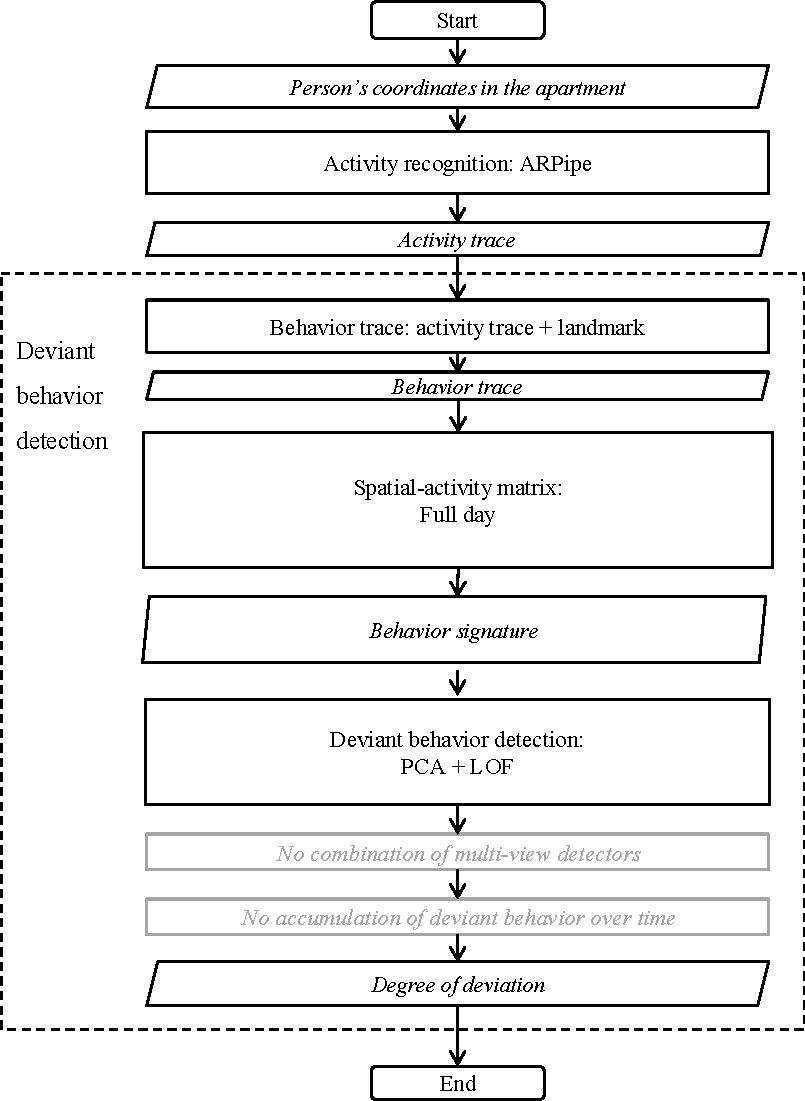
\includegraphics[width=0.8\textwidth]{chap_AAL/stack-AAL.pdf}
\caption{Flowchart of the instantiated unified framework for analyzing daily-living dynamics.}
\label{fig:scheme}
\end{figure*}

\subsection{Sensors and Observations}
\label{sec:overview:data}

We deployed the system in a lab organized as a home apartment, equipped with the Ubisense localization system~\citep{Ubisense}, which allows local positioning by tracking a set of tags attached to a person. The tags were placed at the following locations on the body, as shown in Figure~\ref{fig:tags}: chest, waist, left and right ankle. Each observation vector consists of the absolute $x$, $y$, and $z$ coordinates. 
The observation sequence passed to the next level was a movement trajectory of all the tags in time interval $1 \leq t \leq T$:
$$\mathbf{X}=\{[x_{tag}, y_{tag}, z_{tag}, \cdots]_t | tag \in \{chest, waist, l\_ankle, r\_ankle\}, 1 \leq t \leq T\}.$$

\begin{figure}[!ht]
\centering
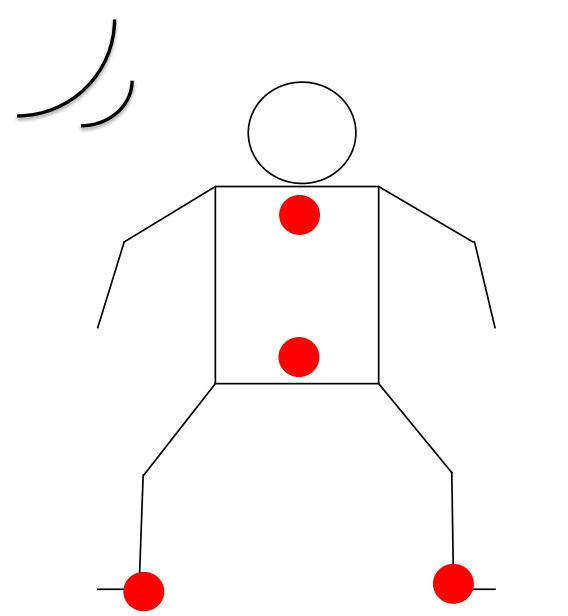
\includegraphics[width=0.3\textwidth, bb=0 0 370 420]{chap_AAL/tags.jpg}
\caption{Ubisense tag placement.}
\label{fig:tags}
\end{figure}



\subsection{Activity Recognition Pipeline}
\label{sec:overview:ar}

\index{activity recognition pipeline}
The raw sensor data are further processed with ARPipe as described in Chapter~\ref{chap:activity_recognition}. First, a median filter is applied to remove the impulsive noise. Next, an iterative constrain satisfaction method that enforces human body constraints between the measured tag positions is applied. Finally, Kalman's filter estimates additional parameters, such as tag velocity.

Activity recognition is performed in three steps. First, we extract tag attributes, such as the $z$ coordinates, all tag velocities, the absolute distances, and the $z$ direction distances between all the tag pairs. Activity recognition omits $x$ and $y$ coordinates because, from the activity-classification point of view, the location of an activity is not important. However, the $x$ and $y$ coordinates are essential for any daily living pattern analysis.

\index{canonical representation}
Second, person postures are classified into one of the following atomic activities: $\mathbb{A}=\{walking, sitting, lying\}$. The feature vector uses canonical representation with window length $W=10$. A new feature window is then obtained after every update, thus overlapping with the previous one, and provides instant classification for each observation vector. We have tested a variety of machine-learning algorithms \citep{Lustrek2009Fall}, including C4.5 decision trees, na{\"i}ve Bayes, SVM, k-NN, bagging, AdaBoost, etc., with SVM offering the highest classification accuracy.

\index{spurious activity transitions}
Third, activity recognition errors that produced spurious activity transitions were reduced using the HMMs \citep{Rabiner1989} as described in Section~\ref{sec:ar:spurious}. Preliminary results indicated that HMMs are superior compared to sequential grammar-based classifiers \citep{Kaluza09Reducing}. The HMM was initialized with $\mathbb{A}=\{walking, sitting, lying\}$ observation symbols, three internal hidden states corresponding to activities, the initial state transition probability $\delta_{ij} = 1/3$, the initial state probability $\pi_i=1/3$, and the output symbol distribution in state $\nu_j(k) = 1$ if $k=j$, otherwise $\nu_j(k)=0$. The parameters were estimated with the Baum-Welch method using $50$ iterations on the training data. The second phase, which finds the optimal hidden state transitions according to the observation sequence, was performed with the Viterbi algorithm. 


%\subsection{Behavior Analysis}
%\label{sec:overview:ba}


%%%%%%%%%%%%%%%%%%%%%%%%%%%%%%%%%%%%%%%%%%%%%%%%%%%%%%%%%%%%%%%%%%%%%%%%%%%%%%%%
\subsection{Behavior Analysis}
\label{sec:ba}

First, the behavior trace is constructed using $\tuple{activity, room}$ tuples. The apartment was divided into logical areas $\mathbb{S}=\{lounge, bedroom, kitchen, toilet\}$ and $(x_{waist},y_{waist})_t$ coordinates were used to determine the area at time step $t$. Then, the behavior trace $\mathbf{b}=\{(a, s)_t|1\leq t \leq T\}$ was passed to the next level.

\index{local outlier factor, LOF}
Behavior signatures were constructed using the spatio-activity matrix approach introduced in Chapter~\ref{chap:signatures} using Algorithm~\ref{alg:SA_matrix}. The matrix dimensionality was further reduced with PCA. Finally, the LOF algorithm \citep{Breunig00lof} assigned each behavior signature an outlier degree, called the local outlier factor (LOF) of a vector. Vectors with a high LOF have local densities smaller than their neighborhood and typically represent stronger outliers, unlike vectors belonging to uniform clusters that tend to have lower LOF values. 

More formally, assume that $\mathcal{B}_T=\{\mathbf{b}_i | 1 \leq i \leq L\}$ is a dataset of behavior traces. First, for each behavioral trace $\mathbf{b}_i$, we compute the spatio-activity matrix $\mathbf{M}_i$ using Algorithm~\ref{alg:SA_matrix}. Next, we compute the principal component vector $\mathbf{m}_i$ (Equations~\ref{eq:PCA-1}--\ref{eq:PCA-4}), and add vector $\mathbf{m}_i$ to a new behavior signature dataset $\mathcal{B}$. Next, for each vector $\mathbf{m}_i$, we compute the $k\_dist_i$ as the distance to the $k^{th}$ nearest neighbor of $\mathbf{m}_i$,  then compute the reachability distance for each vector $\mathbf{m}_i$ with respect to the vector $\mathbf{m}_j$, where $d(\mathbf{m}_i,\mathbf{m}_j)$ is the Euclidean distance from $\mathbf{m}_i$ to $\mathbf{m}_j$, and compute the local reachability density $lrd_i$ of the vector $\mathbf{m}_i$ as the inverse of the average reachability distance based on the $k$ nearest neighbors of the vector $\mathbf{m}_i$. Finally, we compute the $LOF_i$ of the vector $\mathbf{m}_i$ as the ratio of the average local reachability density of $\mathbf{m}_i$'s  $k$ nearest neighbors and the local reachability density of the vector $\mathbf{m}_i$.

\index{detector}
\index{local outlier factor, LOF}
\begin{algorithm}
\caption{Anomaly detection.}
\label{alg:LOF}
\begin{algorithmic}
\REQUIRE set of behavior traces $\mathcal{B}_T=\{\mathbf{b}_i | 1 \leq i \leq L\}$, number of $k$ nearest neighbors
\ENSURE outlier degree for each behavior trace $LOF_i$
\STATE $\mathcal{B} \gets \{\}$
\FOR {$\mathbf{b}_i \in \mathcal{B}_T$}
	\STATE $\mathbf{M}_i \gets spatial\_activity\_matrix(\mathbf{b}_i)$
	\STATE $\mathbf{m}_i \gets PCA(\mathbf{M}_i)$
	\STATE $\mathcal{B} \gets \mathcal{B} \cup \mathbf{m}_i $
\ENDFOR
\FOR {$\mathbf{m}_i \in \mathcal{B}$}
	\STATE $k\_dist_i \gets k\_distance(\mathbf{m}_i)$
	\FOR{$\mathbf{m}_j \in \mathcal{B}, \mathbf{m}_j \neq \mathbf{m}_i$}
		\STATE $r\_dist_{i,j} \gets max(d(\mathbf{m}_i, \mathbf{m}_j), k\_dist_j))$
	\ENDFOR
	\STATE $lrd_i = {k \over { \sum_{\mathbf{m}_j\in kNN(\mathbf{m}_i)}{r\_dist_{i, j}}}}$
	\STATE $LOF_i \gets { {1 \over k}{{ \sum_{\mathbf{m}_j\in kNN(\mathbf{m}_i)}{lrd_j}}} \over lrd_i}$
\ENDFOR
\end{algorithmic}
\end{algorithm}



%
%==========================================================================================
%
\section{Experimental Evaluation}
\label{sec:experiments}

%\subsection{Experimental Setup}
%\label{sec:experimental-setup}
For the prototype deployment we organized a room as an apartment of about~$25$~$m^2$. The apartment was equipped with a bed, a few chairs and tables, and divided into four logical areas: a kitchen, where a person can prepare a meal; a sleeping area; a lounge, where a person can eat a meal, watch TV, write a letter, etc.; and a toilet.



\subsection{Activity Recognition}
\label{sec:experiments:activities}
To build an activity recognition model, we recorded five members of our department. Each participant was recorded performing various activities in three episodes lasting approximately 15--20 minutes each. In total, there were around four hours of recordings. The scenario details are available in \cite{Kaluza2010Agentbased}.

The activity recognition confusion matrix presented in Table~\ref{tab:actRecognition} was obtained with a {\it leave-one-person-out} validation. The left-hand column shows the correct-activity label, and the top row shows the assigned label. The overall classification accuracy is $87.52$\%.

\begin{table}[h!]
\centering
\caption{Confusion matrix for activity recognition. The overall accuracy is $87.52$\%.}
\begin{tabular}{lcccc}
\toprule
True / Labeled [\%] & Lying & Sitting & Standing  \\
\hline
Lying    & 98.99& 0.93& 0.08  \\
Sitting  & 1.67& 67.71& 30.62 \\
Standing & 0.85& 3.27& 95.88 \\
\toprule
\end{tabular}
\label{tab:actRecognition}
\end{table}




\subsection{Anomalous Behavior Detection}
\label{sec:experiments:behavior}

We performed two experiments as follows: the first experiment condensed a full day of activities into scenarios of around half an hour each, while the second test analyzed person behavior in the office for a period of one month.


\begin{figure}[h!t]
 \centering
 \subfloat[Normal day 1]{\label{fig:day-n-1}
 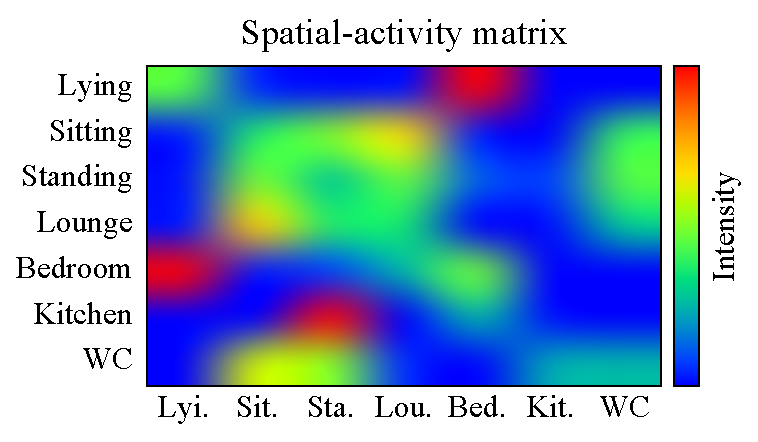
\includegraphics[width=0.50\textwidth]{chap_AAL/matrix-b-3}}
 \subfloat[Normal day 2]{\label{fig:day-n-2}
 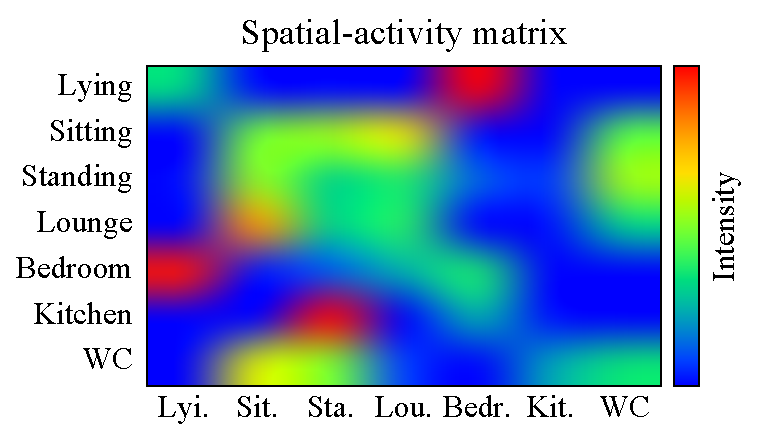
\includegraphics[width=0.50\textwidth]{chap_AAL/matrix-b-4}}

 \subfloat[Normal day 3]{\label{fig:day-n-3}
 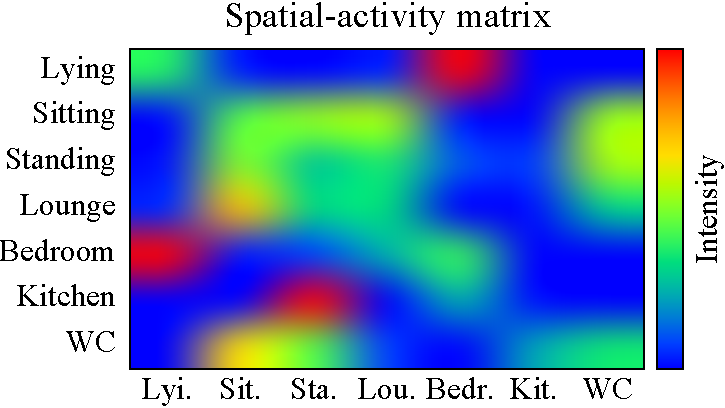
\includegraphics[width=0.50\textwidth]{chap_AAL/matrix-b-5}}
 \subfloat[Normal day 4]{\label{fig:day-n-4}
 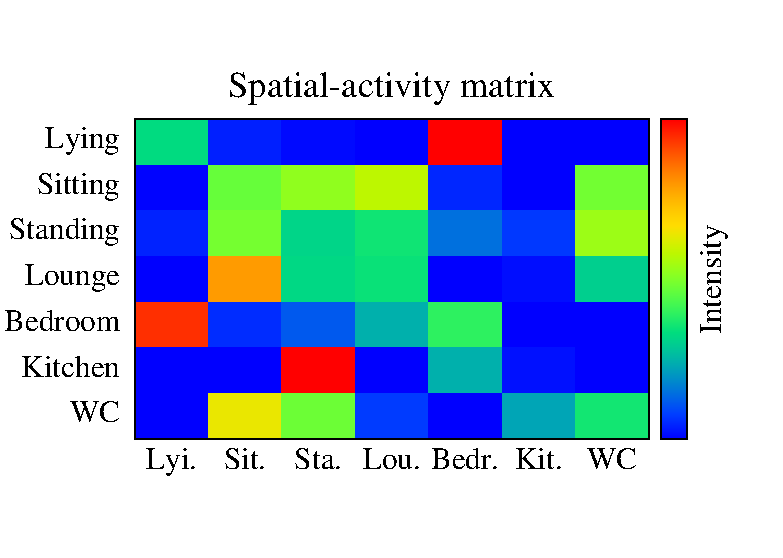
\includegraphics[width=0.50\textwidth]{chap_AAL/matrix-b-6}}

 \subfloat[Slow day]{\label{fig:day-c-1}
 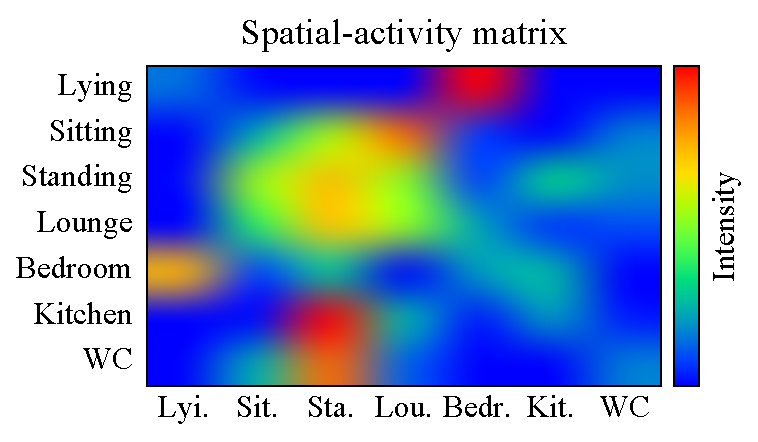
\includegraphics[width=0.50\textwidth]{chap_AAL/matrix-b-c-1}}
 \subfloat[Limping day]{\label{fig:day-c-2}
 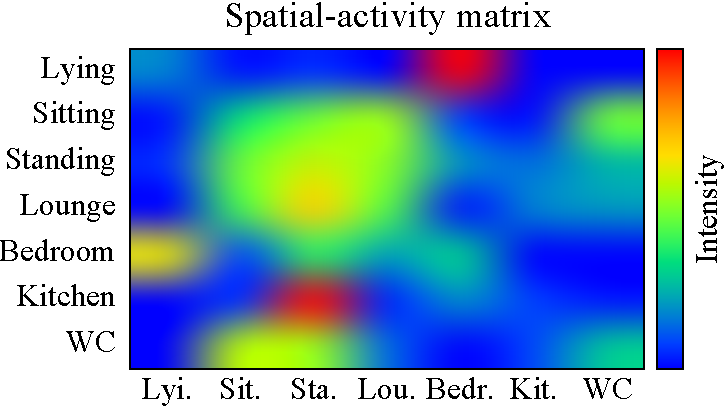
\includegraphics[width=0.50\textwidth]{chap_AAL/matrix-b-c-2}}

 \caption{Behavior matrix visualization for four normal (a,b, c, d) and two deviant days (e, f) of one person.}
 \label{fig:days}
\end{figure}

The first experiments proceeded as follows: the measurements were performed on two people aged between 25 and 32 years, with each day corresponding to a particular scenario, basically the same for each of the persons. The first, usual day represents a typical daily routine for an elderly person. It consists of sleeping, morning routine, breakfast, using toilet/household chores/reading newspaper, preparing and eating lunch, going out/watching TV/household chores/resting, dinner, watching TV/reading, and sleeping. In the second, slow day, the scenario is that the person is not feeling well and, as a consequence, is moving slowly and rests a lot. Such behavior could occur if person had the flu, heart failure, or several other general health problems, either physical or mental. In the third scenario, the person is limping due to, for example, hip pain. As a consequence, the person is also moving slowly and does not stand a lot. The person is not lying as much as on the previous day, but sits more than usual. Each person was given a loose daily scenario and an approximate timing for each activity, but performed it on her/his own. The scenarios were performed and recorded 12 times in total, consisting of eight normal days and four days where the person was not healthy. 
The length of the recordings varied between 25 and 40 minutes. Each recording/day was represented with one behavior trace.


First, we visually compared the usual-day scenario behavior traces with the slow-day and the limping-day scenario behavior traces. Figure~\ref{fig:days} represents spatio-activity matrix visualizations computed from the behavior traces of one person for the four usual days (\ref{fig:day-n-1}--\ref{fig:day-n-4}) and two deviant days (\ref{fig:day-c-1}, \ref{fig:day-c-1}). The spatio-activity matrices plotted in figures \ref{fig:day-n-1}--\ref{fig:day-n-4} captured more or less the same daily dynamics with small variations; for example, there was slightly more standing in the toilet in day~4 (\ref{fig:day-n-4}) than in day~1 (\ref{fig:day-n-1}). The slow day~(\ref{fig:day-c-1}) had an activities over location distribution (lower-right part) quite different compared from the normal days. The most significant feature is an additional orange square, which means that there was more sitting in the lounge. The distribution also deviates during a slow day (\ref{fig:day-c-2}) where, for example, the share of standing is higher than in normal days. 

The difference is even more obvious when PCA is applied. Figure~\ref{fig:PCA} shows the first three PCA components of the behavior traces plotted in Figure~\ref{fig:days}. The four circles `\textbullet' represent the usual days, while the other days are represented by crosses `$\times $'.

\begin{figure*}[t]
\centering
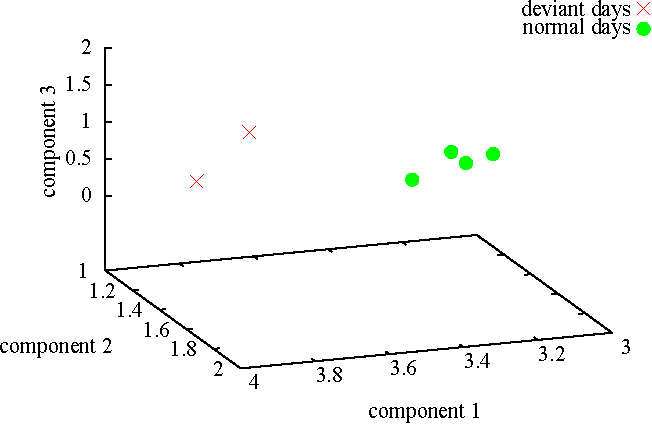
\includegraphics[width=0.8  \textwidth]{chap_AAL/PCA-plot-big}
\caption{Visualization of principal components computed from the matrices shown in Figure~\ref{fig:days}. Normal days are presented with circles, deviation days with  crosses.}
\label{fig:PCA}
\end{figure*}

The anomalous behavioral traces were computed using Algorithm~\ref{alg:LOF}, using {\it leave-one-day-out} validation; that is, one day was used for evaluation while the others were used for training. Table~\ref{tab:LOF-values} shows the LOF values for different values of $k=\{2,3\}$ for all the recordings of both persons. Normal days have $LOF < 1$ in all cases, while the anomalous days have a LOF value significantly higher than $1$.

\begin{table}[h!]
\centering
\caption{LOF values of the behavior traces. A higher value represents a higher outlierness of a behavior trace.}
\begin{tabular}{lcccc}
\toprule
 & $k$=2 & $k$=2 & $k$=3 & $k$=3 \\
Scenario & User 1 & User 2 & User 1 & User 2 \\
\hline
Normal day 1 & 0.619 & 0.615 & 0.887 & 0.963 \\
Normal day 2 & 0.694 & 0.613 & 0.904 & 0.766 \\
Normal day 3 & 0.652 & 0.639 & 0.843 & 0.797 \\
Normal day 4 & 0.601 & 0.743 & 0.832 & 0.841 \\
\hline
Limping day  & 2.369 & 4.270 & 4.519 & 6.465 \\
Slow day     & 3.274 & 2.358 & 5.451 & 4.227 \\
\toprule
\end{tabular}
\label{tab:LOF-values}
\end{table}

In the second experiment, we recorded a member of our department for a period of one month. The person was recorded during working hours, approximately eight hours per day. In this experiment, the person wore only one Ubisense chest tag. The first 10 days were used for training, while the next five days were used for evaluation. Additionally, we recorded three days when the person was experiencing some difficulties: a limping day, where the person limps while he walks; an agitation day, where person occasionally walks around the office for half a minute; and an urinary tract infection day, where the person visits toilets more than usual. In total, there were 18 working days resulting in over 90 recording hours.

The results for five regular and three anomalous days are presented in Table~\ref{tab:LOF-long} for $k={2,3,4}$. The normal working days have LOF values lower than $1$ except on the third day, while the days when the person experienced some kind of difficulty, have significantly higher LOF values.

\begin{table}[h!]
\centering
\caption{LOF values of the long-term test. A higher value represents a higher outlierness of a behavior trace.}
\begin{tabular}{lccc}
\toprule
Day & $k$=1	& $k$=2	& $k$=3 \\
\hline
Regular day 1 & 0.737 & 0.784 & 0.684	\\
Regular day 2 & 0.803 & 0.698 & 0.594	\\
Regular day 3 & 1.618 & 1.579 & 1.281	\\
Regular day 4 & 0.840 & 0.866 & 0.738	\\
Regular day 5 & 0.767 & 0.916 & 0.881	\\
\hline
Limping 		 & 3.706 & 4.820 & 6.216	\\
Agitation 	 & 7.110 & 8.987 & 12.960	\\
Urinary infection & 14.405 & 18.052 & 19.869	\\
\toprule
\end{tabular}
\label{tab:LOF-long}
\end{table}

%%%%%%%%%%%%%%%%%%%%%%%%%%%%%%%%%%%%%%%%%%%%%%%%%%%%%%%%%%%%%%%%%%%%%%%%%%%%%%%%
\section{Discussion}
\label{sec:discussion}

% more tests
%Although the initial results are promising, more realistic, long-term tests are needed to verify the performance of the newly designed method, and further improve it. However, the first results suggest that with further modifications the novel method for daily-living dynamics might prove as useful as indicated. 

% Different periods
In these experiments, we selected one day as a default unit, but in general, the approach can be applied to various period lengths. Furthermore, monitoring the behavior with different granularities by using different periods simultaneously; for example, half a day, a day, a week, or a month, would allow us to detect behavior changes that occur with different pace.

% HMM can model a single 
It should be noted that the task is based on combining activities and spatial information; therefore, applying a uniform method, such as HMMs, is not feasible. The novel method explains the two concepts by combining several existing algorithms, and specializing them for the particular task. In addition, HMMs must estimate the model learning phase parameters, whose quality depends on the labeled data amount \citep{Rabiner1989}. 

% Visulization has two functions
The spatio-activity matrix visualization can be used in two ways. First, it enables visual anomalous behavior detection; by examining the matrices, one cannotice changes in behavior dynamics. Second, it explains those cases when the automatic procedure detects anomalous behavior patterns.

% embedded sensors
The final remark concerns the type of sensors used in the experiments. Even though our approach was evaluated with wireless location sensors (that is, Ubisense), it can be applied to any sensor type from which it is possible to locate and recognize activities; for example, one can use embedded sensors as shown by \cite{Cook2012} and \cite{Storf}. 
%In fact, our future plans include an extensive experiment in an environment with embedded sensors.

%%%%%%%%%%%%%%%%%%%%%%%%%%%%%%%%%%%%%%%%%%%%%%%%%%%%%%%%%%%%%%%%%%%%%%%%%%%%%%%%
\section{Conclusion}
\label{sec:conclusion}

The main goal of this chapter was to deliver a solution whereby a caregiver can constantly and remotely observe a person's daily behavior in an efficient and unobtrusive manner. We demonstrated how to apply the unified detection framework for transforming behavior traces into a spatio-activity matrix, which captures daily behavior and presents a visualization and explanation of behavior deviations. 

We proposed a method for automatic discovery of anomalous daily behavior, which consists of feature extraction based on PCA and outlier detection implemented with the LOF algorithm. The outputs can be directly used to signal a warning to the person and caregivers, providing information that the person dynamics has changed significantly along with a relevant explanation. 
%
The experimental results showed that the proposed approach is successful in discriminating normal days from days where the person's well-being is affected. 

% FUTURE WORK
The method has not been tested thoroughly yet. Further realistic, long-term tests with the target group are needed to verify the newly designed method's performance, and to further improve it. However, the first results are quite promising; with further modifications, the novel method for daily living dynamics might prove useful as indicated. 


%%%%%%%%%%%%%%%%%%%%%%%%%%%%%%%%%%%%%%%%%%%%%%%%%%%%%%%%%%%%%%%%%%%%%%%%%%%%%%%%
%\section*{Acknowledgments}
%\label{sec:conclusion}
%This work was partly supported by the Slovenian Research Agency under the Research Programme P2-0209 Artificial Intelligence and Intelligent Systems, and partly from the European Community's Framework Programme FP7/2007-2013 under grant agreement No. 214986. We would like to thank Mitja Lu{\v s}trek, Erik Dovgan, Bo{\v z}a Cvetkovi{\' c}, Violeta Mirche\-vska for suggestions, discussions and help with the programming. 
\newpage \thispagestyle{empty}

%!TEX root = thesis.tex

%
%==========================================================================================
%
\chapter{Surveillance Domain}
\label{chap:lax}
% 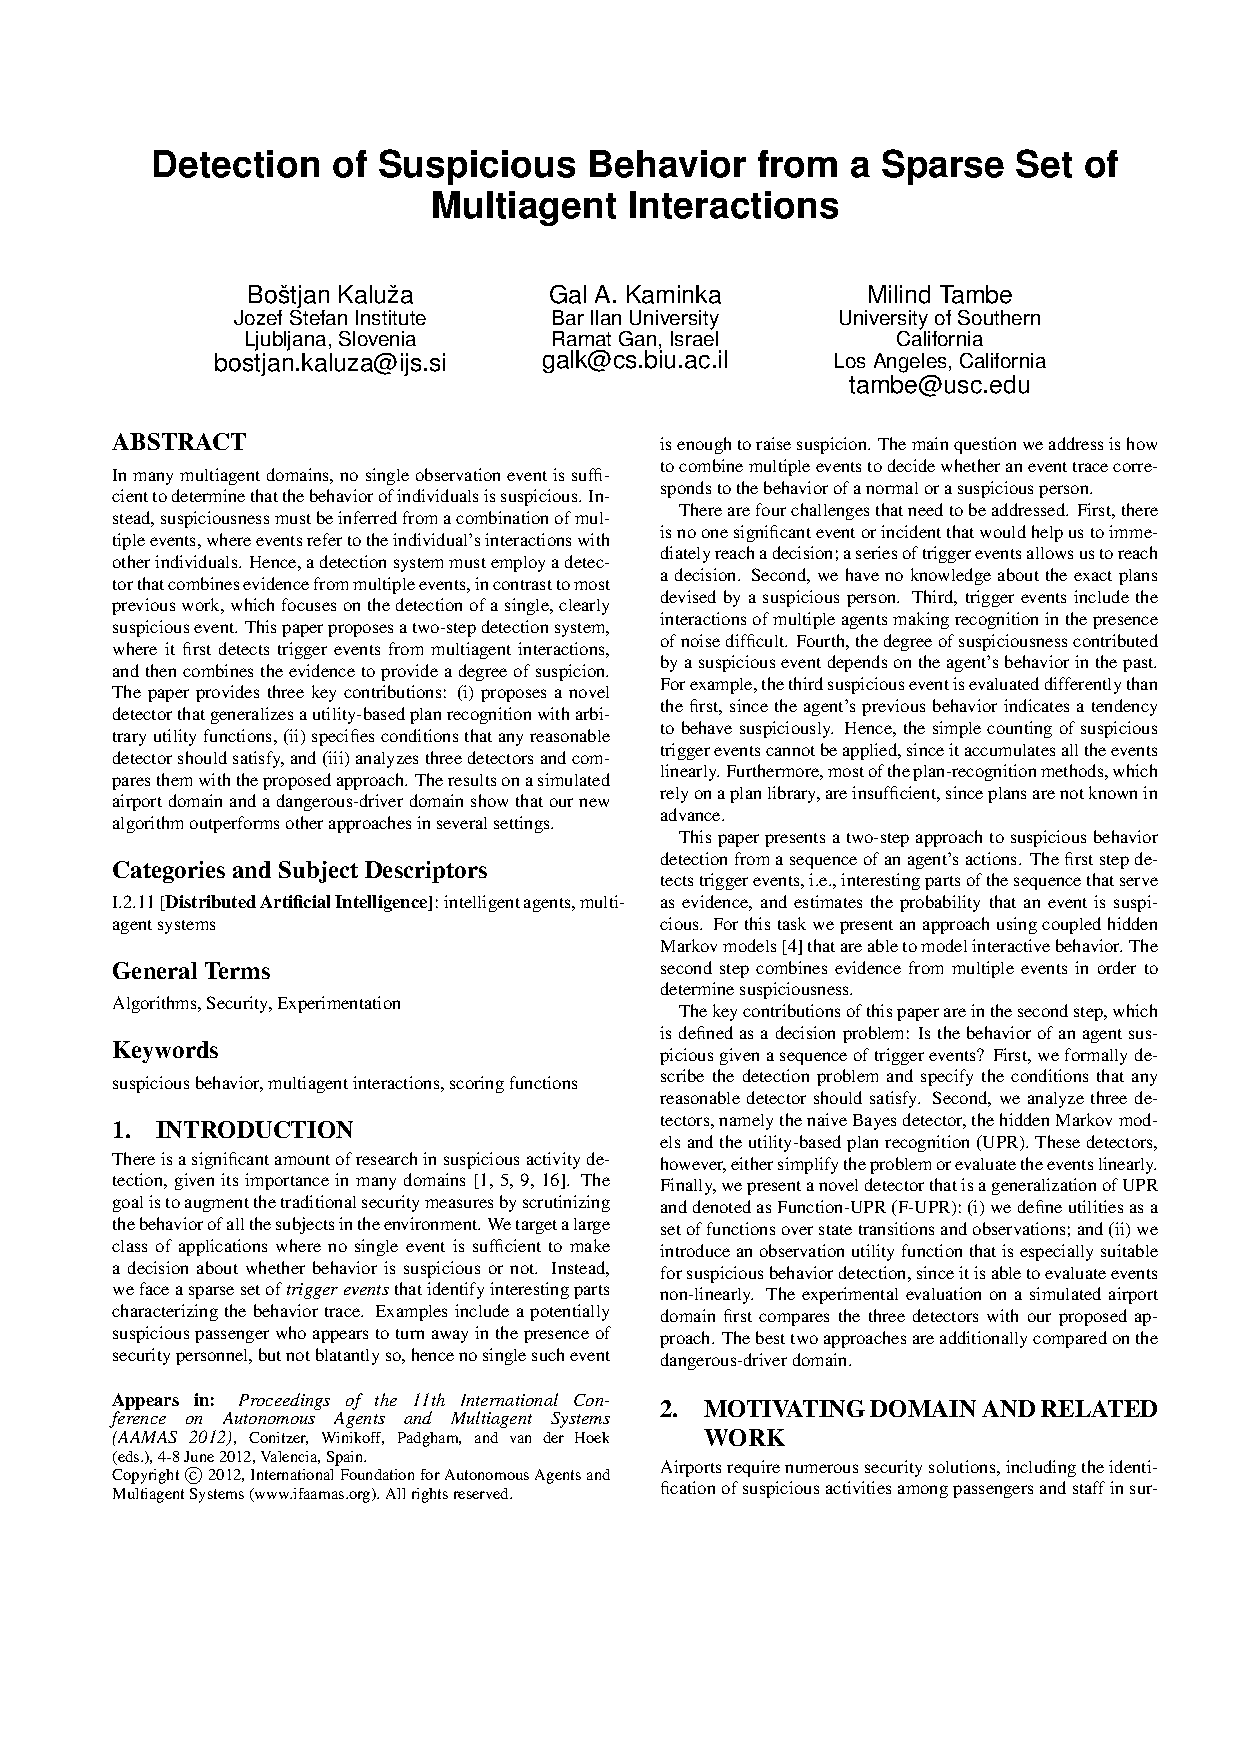
\includepdf[pages=1-last, fitpaper=true, addtotoc={
% 1, section, 1, {Detection of Suspicious Behavior from a Sparse Set of Multiagent Interactions}, sec:aamas, %
% 1, subsection, 2, {Introduction}, sec:aamas:intro, %
% 1, subsection, 2, {Motivating Domain and Related Work}, sec:aamas:related, %
% 2, subsection, 2, {Definitions and Assumptions}, sec:aamas:definitions, %
% 3, subsection, 2, {Problem Definition}, sec:aamas:problem, %
% 4, subsection, 2, {Detectors}, sec:aamas:detectors, %
% 	4, subsubsection, 3, {Naive Bayes Detector}, sec:aamas:detectors:bayes, %
% 	4, subsubsection, 3, {Hidden Markov Models}, sec:aamas:detectors:hmms, %
% 	5, subsubsection, 3, {Utility-Based Plan Recognition}, sec:aamas:detectors:upr, %
% 	%5, subsubsubsection, 4, {Utilities as Potential Functions}, sec:aamas:detectors:upr:potential, %
% 	%5, subsubsubsection, 4, {Observation Utility for Suspicious Behavior Detection}, sec:aamas:detectors:upr:exponential, %
% 6, subsection, 2, {Experimental Evaluation}, sec:aamas:experiments, %
% 	6, subsubsection, 3, {Airport Domain}, sec:aamas:experiments:airport, %
% 	8, subsubsection, 3, {Catching a Dangerous Driver}, sec:aamas:experiments:driver, %
% 8, subsection, 2, {Conclusion}, sec:aamas:conclusion, %
% 8, subsection, 2, {References}, sec:aamas:references %
% }]{article/AAMAS2012.pdf}

This chapter focuses on two applications in surveillance domain, where the goal is to detect suspicious agents in the environment. In particular, the chapter targets a large applications class where no single event is sufficient to gauge whether or not agent behavior is suspicious. Instead, we face a sparse set of \emph{trigger events} that identify interesting parts in behavior trace. The first application considers suspicious passenger detection at an airport, while the second application tackles dangerous driver detection.
%The main tasks are, hence, first to detect trigger events, and then combine them over time into a reliable behavior evaluation.


\section{Introduction and Background}


There is significant suspicious activity detection research, given its importance in many domains~\citep{Arsic, Duong2005, Helman1993, Vaswani}. The goal is to augment the traditional security measures by scrutinizing the all subjects' behavior in the environment. 
%
%We target a large class of applications where no single event is sufficient to make a decision about whether behavior is suspicious or not. Instead, we face a sparse set of \emph{trigger events} that identify interesting parts characterizing the behavior trace.  %Examples include a suspicious passenger at an airport that immediately flees the area when noticed by security or a reckless driver zigzagging across two lanes. 
%Examples include a potentially suspicious passenger who appears to turn away in the presence of security personnel, but not blatantly so, hence no single such event is enough to raise suspicion.
The main question we address is how to combine multiple events to decide whether an event trace corresponds to the behavior of a normal or a suspicious person. 





%There are four challenges that need to be addressed. 
%First, there is no one significant event or incident that would help us to immediately reach a decision; a series of trigger events allows us to reach a decision. Second, we have no knowledge about the exact plans devised by a suspicious person. Third, trigger events include the interactions of multiple agents making recognition in the presence of noise difficult. 
%Fourth, the degree of suspiciousness contributed by a suspicious event depends on the agent's behavior in the past. For example, the third suspicious event is evaluated differently than the first, since the agent's previous behavior indicates a tendency to behave suspiciously. 
%Hence, the simple counting of suspicious trigger events cannot be applied, since it accumulates all the events linearly. Furthermore, most of the plan-recognition methods, which rely on a plan library, are insufficient, since plans are not known in advance.


In the airport scenario, various systems were introduced to automatically detect some of the threats, such as leaving objects behind~\citep{Hongeng2003}, suspicious trajectory paths~\citep{Vaswani}, 
%suspicious transportations~\cite{Arsic},  
thefts~\citep{Hongeng2003}, and vandalism acts and fights~\citep{AdvisorProject}. 
There is also a commercially available system~\citep{IBMsmart} that is able to detect such events as running passengers, climbing over a fence, etc.  
However, these approaches mainly deal with the detecting single, clearly suspicious incidents and do not address accumulating suspicion.


%BACKUP PARA: There are four challenges that need to be addressed. First, there is no significant event or incident that would help us to immediately reach a decision; a series of trigger events over time establishes our decision with accumulating effect. This would normally do for the use of plan recognition methods, but unfortunately, the second challenge is that we have no knowledge about the exact plans devised by a suspicious person. Thus most of the plan recognition methods, which rely on a plan library, are insufficient. Third, trigger events include interactions of multiple agents making recognition under noise difficult. Fourth, evaluation of an event changes degree of suspiciousness with the number of detected suspicious events in the past; that is, two suspicious events are evaluated differently according to individual's behavior in the past. Hence, simple counting of suspicious trigger events cannot be applied, since it accumulates all events linearly.



%These challenges disallow direct application of plan recognition as they assume that the plan library is known in advance. Furthermore, simple counting of suspicious trigger events disallows non-linear accumulation. 
%assigned degree of suspiciousness
%The main question we are addressing is how to decide whether an event trace corresponds to behavior of a normal or a suspicious agent.
%interesting parts from \emph{trigger events}, that is interesting events that help to establish our decision. 
%TODO: UPDATE. The current approaches can be divided into three groups. The first group focuses on significant events, we call them incidents, that are used as the evidence of suspicious behavior (for example, leaving object behind [?], vandalism acts[], running passengers[]). Second, trajectory-based approaches examine trajectory shape to identify suspiciousness.  

%The main question we are addressing is how to decide whether an event trace corresponds to behavior of a normal or a suspicious agent. Standard approaches include modeling both normal and suspicious behavior traces of a single agent using probabilistic models, plan recognition, etc. However, behavior of an agent in a multiagent environment is influenced by other agents, which is usually not captured in such models. Instead, we focus on \emph{trigger events} that identify interesting parts characterizing the behavior trace. Trigger events can present either positive or negative belief about the motivating goal and tend to be noisy; it is not clear if a person emitting suspicious events is indeed acting suspiciously. They also involve interactions of multiple agents making recognition under noise difficult. In many cases no single action or event is sufficient to reveal adversary intentions, but a collection of events enables the observer to infer the underlying intentions. Moreover, our belief that an individual is acting suspiciously  increases with the number of detected suspicious events non-linearly; that is, individual's behavior in the past affects current evaluation.


%Problems with current approaches\\
% - modeling complete behavior traces is not feasible\\
% - we establish a formal framework for evaluating event traces and show where are the problems
% - it is hard to do take history into account\\

%Our solution\\
% - focuses on trigger events\\
% - heuristic approach
% - defines a family of \emph{well-behaved} evaluation functions\\
% - proposes an instance of function\\
This chapter addresses how to instantiate the unified detection framework to detect trigger events, that is, interesting trace parts  that serve as evidence, and combine evidence from multiple events in order to estimate suspicion. 
%The first task is based on an approach using coupled hidden Markov models~\cite{Brand} that are able to model interactive behavior. The second task combines evidence from multiple events in order to determine suspiciousness.
%
%The key contributions of this paper are in the second step, which is defined as a decision problem: {Is the behavior of an agent suspicious given a sequence of trigger events?} First, we formally describe the detection problem and specify the conditions that any reasonable detector should satisfy. Second, we analyze three detectors, namely the na{\"i}ve Bayes detector, the hidden Markov models and the utility-based plan recognition (UPR). These detectors, however, either simplify the problem or evaluate the events linearly. Finally, we present a novel detector that is a generalization of UPR and denoted as Function-UPR (F-UPR): (i) we define utilities as a set of functions over state transitions and observations; and (ii) we introduce an observation utility function that is especially suitable for suspicious behavior detection, since it is able to evaluate events non-linearly.
%
The experimental evaluation of a simulated airport application first compares the three detectors from Chapter \ref{chap:accumulation} (Section~\ref{sec:acc-detectors}) with our proposed approach (Section~\ref{sec:FUPR}). The best two approaches are additionally compared in the dangerous-driver application.

%The experimental evaluation on a simulated airport domain first compares the three detectors with our proposed approach. We also compare it to an approach that uses a complete sequence of actions (instead of a sequence of trigger events). \hl{Finally, the best two approaches are compared on the dangerous-driver domain}.


%The experiments in a simulated multiagent environment show that the proposed approach outperforms other approaches in several settings. 
%UPR and its generalization F-UPR are finally compared on the dangerous driver domain confirming the results.


% and assigns them probabilities that  formally defines the problem within a Bayesian framework, analyzes four algorithms to address it, and introduces a new algorithm able to address the abovementioned challenges.
%
%
%This paper introduces a Bayesian plan recognition framework as a formal definition of the problem, analyses four detectors and introduces a new detector that addresses the above-mentioned challenges. 
%The paper introduces three key contributions. 
%First, we show the optimal detection within the proposed Bayesian framework and discuss why it is not feasible in practice. Next, we introduce a Na{\" i}ve Bayes approximation as well as two detectors, namely Hidden Markov Models [] and Utility Plan Recognizer []. Unfortunately, these detectors either over-simplify the approximation, do not take into account history, and accumulate evaluation linearly. Finally, we introduce a family of \emph{scoring functions} for evaluating event traces and propose a heuristic function that evaluates an event trace non-linearly. 
%Experimental results in a simulated airport domain 

%The key contributions of this paper are (1) introduction of a Bayesian suspicious detection framework, (2) analysis of four detectors

%five algorithms. The It shows that the optimal detector within Bayesion framework  solution whithin for evaluating event traces and evaluation (that is, whether a trace is produced by a suspicious agent) does take into account interactions between events. More precisely, evaluation of an event depends not only on the current time step but also on the events in prior time steps. 
%We propose a heuristic approach that defines a family of \emph{well-behaved} scoring functions that interpret an event trace to produce a score presenting overall suspicion that the trace corresponds to the behavior of a suspicious agent. The key component is that the events are evaluated according to the behavior of the agent in the past. We present a set of scoring functions that satisfy that conditions.


%Verification procedure\\
% - evaluation on motivating domain -- airport scenario\\
% - proposes event detection procedure\\
% - compare different approaches using simulation
%Experimental evaluation on a simulated airport domain first compares the three detectors with our proposed approach. We also compare it to an approach that uses a complete sequence of actions (instead of a sequence of trigger events). The experiments in a simulated multiagent environment show that the proposed approach outperforms other approaches in several settings.






%%%%%%%%%%%%%%%%%%%%%%%%%%%%%%%%%%%%%%%%%%%%%%%%%%%%%%%%%%%%%%%%%%%%%%%%%%%%%%%%%%%%%%%%%%%


% \section{Related Work}
% \label{sec:domain}
% %A dramatic increase in air travel in recent years has made every airport a potential terror target, hence intense security is a necessary requirement. This global transportation system is no longer considered as safe, but rather as a potential liability exposed to terrorist attacks and other criminal activities, such as drug and contraband trafficking. Airports require vast security solutions including the identification of suspicious activities amongst passengers and staff in surrounding areas.
% \noindent 
% Airports require numerous security solutions, including the identification of suspicious activities among passengers and staff in surrounding areas.
% %
% Our goal is to monitor passengers during the time they spend at the airport and to detect those that indicate a high level of stress, fear or deception. It is reasonable to assume that there is a camera network to track a passenger throughout the airport. We focus on a task where no single event is sufficient to identify a suspicious passenger, but a series of events establishes the decision over time. The detection of events might be limited due to noise or an inability to extract some features (for example, using a ceiling-mounted camera one can extract the trajectory of a passenger, but not facial expressions), hence a normal person may appear suspicious (and vice versa).
% Also, a precise plan of the suspicious passenger is not known in advance. 
% %
% %Observer might be limited due to various reasons such as inability to detect characterizing features and noisy trigger-event detectors.
% %
% Other domains of interest may include identifying a reckless driver executing dangerous (but still legal) maneuvers~\cite{Avrahami-Zilberbrand2009}, detecting a pirate vessel that plans to capture a transport vessel and therefore avoids security patrols, etc. 

%To run proof-of-concept tests we consider a simulated environment due to several reasons. First, a simulation is controllable and repeatable in terms of ensuring statistical relevance. Second, obtaining real-world data with annotated suspicious behavior might present a difficulty in terms of cost and amount of data required to create a statistically representative dataset. In practice there are tens of hours of several hundred people with only a few instances of suspicious behaviors. Third, a simulator enables the control of the amount of noise that is otherwise introduced by various vision systems (occlusions, false detections, etc.). And last, real-world data in security domain present a difficulty due to privacy issues, confidentiality and national security concerns.

%To run proof-of-concept tests we consider a simulated environment, mainly to avoid difficulties due to privacy and confidentiality issues and as well as due to absence of annotated suspicious behavior in real world. A simulator also enables to control the amount of noise otherwise introduced by various vision systems (occlusions, false detections, etc.), and provides  controllable and repeatable situations. Experiments in this paper use ESCAPES~\shortcite{Tsai2011}, a state-of-the-art multiagent simulator for airport evacuations with several types of agents exhibiting behaviors of regular travelers, authorities, and families. We assume that behavior of the agents corresponds to the behavior of real passengers at the airport.

%
%ESCAPES consists of two parts, a 2D environment based on the open-source project OpenSteer~\cite{OpenSteer}, outputting agents' physical and behavioral information into files, and a 3D visualization component using the Massive Software~\cite{Massive}. 
%The first part consists of agents interacting in an environment, outputting their physical and behavioral information into files later used in a customized Massive extensions to generate 3D movies of the scenarios.
%In one scenario, they modeled the Tom Bradley International Terminal at Los Angeles International Airport including terminals and shops as a realistic simulation environment. This served as our playground for introducing suspicious behaviors prior to an evacuation occurring.


%In many cases, the extra scrutiny is a casual conversation with a TSA behavior officer that shows someone is innocent, 

%"behavioral surveillance" has "enormous potential for violating" privacy.

%"The shortcoming is, we don't know how many people are showing suspicious behaviors and aren't being noticed," Ekman said.

%Although observers can perceive whether someone appears anxious or is acting deceptively, they can't tell whether that person is planning an attack or something such as an extramarital affair, Levenson said.

%Our goal is to monitor a passenger 

%Airport security has increased drastically in recent years.
%Nowadays the security at the airports 
%Motivation...



%\section{Related Work}
%\label{sec:RelatedWork}


%An approach for monitoring behavior of passengers over longer periods of time relies upon security personnel such as behavior detection officers (BDOs) that patrol airport to identify passengers who display \emph{involuntary physical and physiological actions} (US Transportation Security Administration (www.tsa.gov) trained and deployed BDO officers at 161 US airports). In this context we strive to observe passengers for the whole time they spend at the airport. We are focused on trigger events in terms of actions, events and incidents that can be potentially suspicious in order to identify individuals who exhibit behaviors that indicate high levels of stress, fear or deception.

%Describe differen t approaches
%\noindent
%There are two approaches to detecting deviant behavior~\cite{Avrahami-Zilberbrand2009}: \emph{suspicious} and \emph{anomalous} behavior detection. The first approach assumes a behavior library that encodes \emph{negative behavior}, and thus recognizing observed behavior corresponds to identifying a match in the library. The second approach uses the behavior library in an inverse fashion, meaning that the library encodes only \emph{positive behavior}. When an observed behavior cannot be matched against the library it is considered as anomalous. Several approaches have been proposed to tackle the problem either way. % and the literature is vast. 
% In the airport scenario various systems were introduced to automatically detect some of the threats, such as leaving objects behind~\cite{Hongeng2003}, suspicious trajectory paths~\cite{Vaswani}, 
% %suspicious transportations~\cite{Arsic},  
% thefts~\cite{Hongeng2003}, and vandalism acts and fights~\cite{AdvisorProject}. 
% There is also a commercially available system~\cite{IBMsmart} that is able to detect events such as running passengers, climbing over a fence, etc.  
% However, these approaches mainly deal with the detection of single incidents, which are clearly suspicious. They do not address accumulating suspicion as we do.
% % or monitor only a part of the premises. 

% %We focus to related research within recognition from multiple events emphasasing  probabilistic models and plan recognition. 
% Another area of related work includes hidden Markov models (HMMs)~\cite{Rabiner1989} that are widely used in traditional activity recognition for modeling a sequence of actions.  Brand et al.~\cite{Brand} introduced coupled HMMs as an extension with multiple hidden interacting chains that are able to model interactive behavior. 
% %Moreover, layered HMMs~\cite{Oliver2004} and hierarchical HMMs~\cite{Fine1998} can handle activities that have hierarchical structure, for example, activity recognition from trajectories \cite{Nguyen2005}. 
% Duong et al.~\cite{Duong2005} focused on the duration of activities and introduced switching hidden semi-Markov models that provide probabilistic constraints over the duration of plans, and applied them to the detection of anomalies in the activities of daily living. 
% %Vaswani et al.~\cite{Vaswani} introduced Continuous State HMMs for modeling trajectories in order to detect anomalous activities. 
% Although widely used, HMMs may become inadequate when actions are more complex or have long-term temporal dependencies~\cite{KollerFriedman2009}. 
% %
% %Even though our approach is completely different from HMMs, we further discuss some variations of HMMs in Section~\ref{sec:Experiments}.% and compare them with ESPY.


% %\subsection{Utility-based Plan Recognition}
% %\label{sec:UPR}
% Plan recognition algorithms may use a hybrid approach for suspicious activity recognition. A symbolic plan recognizer is used to filter consistent hypotheses, passing them to an evaluation engine, which focuses on ranking. Geib and Goldman presented PHATT~\cite{Geib2009}, a probabilistic approach based on tree grammars able to cope with interleaved goals, partially ordered plans, and failed observed actions. Sukthankar and Sycara~\cite{Sukthankar-AAAI2008} addressed plan recognition for multiagent teams, where plans were ordered by linear accumulation of observed actions consistent with the plan.
% Another approach is presented by Avrahami-Zilberbrand and Kaminka~\ref{Avrahami-Zilberbrand2009, Avrahami-Zilberbrand2007}. Utility-based Plan Recognition (UPR) introduces utility to the observer in selecting the recognition hypotheses. The main strength of UPR is that it can incorporate an observer's bias to events with a low likelihood, for example, the a-priori probability for planting a bomb is very low, but detecting it has a high expected utility. We further discuss this approach in Section~\ref{sec:UPR}. 
% %Other approaches based only on symbolic plan recognition This would normally do for the use of plan recognition methods, but unfortunately, the second challenge is that we have no knowledge about the exact plans devised by a suspicious person.

% Furthermore, intrusion detection systems analyze a variety of person activities to identify suspicious computer activities. Helman and Liepins~\cite{Helman1993} proposed an intrusion detection system that provides a rating for computer activities, demonstrating frequency estimator and matching rules. Esponda et al.~\cite{Esponda2004} analyzed tradeoffs between positive and negative activity patterns in the library and presented an approach based on partially matching rules. These approaches similarly address the problem of how to decide whether a person's activity is suspicious, but differ significantly in using a different approach to match and assess behavior. 

%Our approach in a similar way evaluates the events using utilities but with two key differences: (i) utility functions dynamically change in order to adapt to the behavior history of the observed agent; and (ii) evaluation process in ESPY introduces the forgetting mechanism in order to deal with noise.




%%%%%%%%%%%%%%%%%%%%%%%%%%%%%%%%%%%%%%%%%%%%%%%%%%%%%%%%%%%%%%%%%%%%%%%%%%%%%%%%%%%%%%%%%%%

% \section{Definitions and Assumptions}
% \label{sec:definitions}
% \noindent
% Our methods are general, but for illustrative purposes we will make use of the airport domain to provide examples. We treat subjects as agents in a multi-agent environment. At this point we assume that we can perfectly observe their actions. 
% \begin{definition}
% 	\emph{Action} $a_t$ is a tuple of observed feature values\\ $\langle f_1, ..., f_n \rangle$ that describe state of an agent at a given time stamp $t$.
% \end{definition}
% %
% \begin{definition}
% 	\emph{Action trace} $\avec{l}$ is a totally-ordered sequence of $l$ actions $\avec{l}=(a_1,a_2,...,a_l)$.
% \end{definition}
% %
% \begin{definition}
% 	\emph{Trigger event} $x^{i,j}=(a_i, ..., a_j)$ is a subsequence of action trace $\avec{k}$ (s.t.\  $1 \leq i < j \leq k$). A trigger event $x$ is described by probabilities that the corresponding subsequence is suspicious $s(x)$ and normal $n(x)$.
% \end{definition}
% %
% \begin{definition}
% 	\emph{Event trace} $\xvec{k}$ is a totally-ordered sequence of $k$ trigger events $\xvec{k}=(x_1,x_2,...,x_k)$.
% \end{definition}

% We address the problem of suspicious behavior detection in two steps, as shown in Figure~\ref{fig:architecture}. The first step analyzes an action trace and the surrounding environment to detect trigger events that characterize its interesting parts. The event trace then enters the second step, where it is evaluated. If the evaluation result exceeds a threshold value or is large relative to other evaluations of the event traces, then it is considered as suspicious.

% \begin{figure}[!ht]
% \centering
% \includegraphics[width=0.7\linewidth, bb=34 10 523 530]{chap_surveillance/flowchart.pdf}
% \caption{Two-step detection of suspicious behavior: (1) detection of trigger events and (2) detection of suspicious behavior.}
% \label{fig:architecture}
% \end{figure}


% %\subsection{Trigger Events}
% %\label{sec:events}
% %\noindent
% Trigger events can be any kind of partial observations we are able to extract from the domain. In the airport domain, one can focus on people exhibiting indications of suspicious behavior, such as taking photos of critical infrastructure, revisiting the same location, evading the area when noticed, standing in customer service but not requesting the service, etc. 
% %We focus on a rather novel descriptor we were unable to find in the literature on suspicious behavior detection at the airport. 
% We focus on a well-known detector obtained from conversations with domain experts. %and commonly used by behavior detections officers\footnote{An approach for monitoring behavior of passengers over longer periods of time relies upon security personnel such as behavior detection officers (BDOs) that patrol airport to identify passengers who display \emph{involuntary physical and physiological actions}. US Transportation Security Administration (www.tsa.gov) trained and deployed BDO officers at 161 US airports.}.
% We observe the interactions between agents at the airport, more precisely, we are interested in how a passenger behaves in the presence of a uniformed authority figure. A person exposed to a high level of stress produces behavior that indicates fear, anxiety, pressure, tension, deception, etc. Hence, it is rational for the suspicious agent to minimize contacts with the authorities. Note, that no single avoidance is enough to raise a flag, but many such events put together cause the person to be treated as suspicious. 

% %This results in a set of partial observations describing interactive behavior of a passenger. The recognition process first extracts all interactions between passengers and authority figures inside a given radius, producing a set of trajectory pairs that are transformed to relative presentation. 

% A trigger-event detection able to identify interactive behavior may rely on coupled hidden Markov models (CHMMs), which are briefly described below. The reader is referred to~\cite{Brand} for details; the CHMMs are not the main contribution of the paper.
% %To differentiate between authority-regular and authority-suspicious interactions we present an approach based on coupled hidden Markov models (CHMM). 
% %
% The observations consist of two action traces, namely the action trace of the agent of interest and the action trace of an authority agent when they are within some predefined radius. The CHMMs are able to model the complex, interactive behavior by two HMM chains, where the hidden states from one chain directly impact on the hidden states from the other chain. Figure~\ref{fig:CHMMs} illustrates the CHMM for a pair of action traces with length $l=3$. The current state $Q_t^A$ of agent $A$ is affected by both its previous state $Q_{t-1}^A$ and previous state $Q_{t-1}^B$ of the agent $B$ (similarly $Q_t^B$ is affected by $Q_{t-1}^B$ and $Q_{t-1}^A$). Each state $Q_i$ also impacts the corresponding observation state $Y_t$. For example, if the authority agent moves toward the suspicious agent, the next state of the latter takes this into account and produces an action for an avoidance maneuver. 
% %The joint distribution for a pair of traces of length $k$ can be obtained by unrolling the network until we have $k$ slices, and them multiplying together all of the conditional probability distributions. 


% \begin{figure}[!ht]
% \centering
% \includegraphics[bb=0 0 595 830, angle=-90, width=0.5\linewidth]{chap_surveillance/chmm.pdf}
% \caption{An example of CHMM for a pair of action traces with length $l=3$.}
% \label{fig:CHMMs}
% \end{figure}

% A regular passenger may not turn or do anything different in the presence of authorities, while a suspicious person will (although as described below, an observer may not have perfect observability). Therefore, we create and train two CHMMs: $\hat{N}_I$ models the interactions produced by authorities and regular passengers, while $\hat{S}_I$ models the interactions produced by authorities and suspicious passengers. For a new event (interaction) $x$ we compute the posterior probability that the event is generated with both models yielding $\hat{n}_I(x)=\Prob\{x|\hat{N}\}$ and $\hat{s}_I(x)=\Prob\{x|\hat{S}\}$, respectively. %We also experimented with more complex CHMM structures including other features such as relative speed and distance, but the results were comparable or even worse.


% %As a trigger event we also extract all turns in absence of authority when the trajectory curvature exceeds a threshold value. Probabilities that a turn event was generated by suspicious $\hat{n}_T(x)$ or regular passenger $\hat{s}_T(x)$ is acquired with frequentist estimator from the learning set $D_l$.
% %
% %
% %The second architecture (Figure~\ref{fig:CHMM-3}) incorporates additional information in the form of a model of relative speed between two agents. This model directly impacts the states of both agents. The idea behind this architecture is to improve recognition results with an additional information.
% %
% %Note that for an interaction of length $T$ the architectures presented in Figure~\ref{fig:CHMMs} are unrolled to $T$ slices. %(similar as in Figure~\ref{fig:HMM-4}). 


% %\begin{figure}[!ht]
% %\centering
% %\subfigure[]{
% %\includegraphics[width=0.25\linewidth]{CHMM-2}
% %\label{fig:CHMM-2}
% %}
% %\subfigure[]{
% %\includegraphics[width=0.25\linewidth]{CHMM-3}
% %\label{fig:CHMM-3}
% %}
% %\caption{CHMM presented as 2-sliced DBN: (a) modeling actions of two agents and (b) modeling both actions and relative speed.}
% %\label{fig:CHMMs}
% %\end{figure}




% %%%%%%%%%%%%%%%%%%%%%%%%%%%%%%%%%%%%%%%%%%%%%%%%%%%%%%%%%%%%%%%%%%%%%%%%%%%%%%%%%%%%%%%%%%%


% \section{Problem Definition}
% \label{sec:problem}
% \noindent
% This section formally analyzes how to evaluate a sequence of trigger events. We leverage the Bayesian framework for intrusion detection~\cite{Helman1993} for the problem definition.
% At each time step $t$ we observe an event $x_t$, generated by a hidden stochastic process $H$. Now suppose that $H$ is a mixture of two auxiliary stochastic processes, namely the normal process $N$ and the suspicious process $S$ that correspond to a normal and a suspicious passenger. The random variable $y_t=0$ if $x_t$ is generated by $N$ and $y_t=1$ if $x_t$ is generated by $S$. Since a suspicious passenger always emits a suspicious event (and a normal person a normal event), $y$ for a specific agent does not change over time. In reality, there can be many subprocesses contributing to each of $N$ and $S$; that is, many normal persons with different behavior patterns; however, here we assume only a single $N$ and a single $S$ that capture all the variability. 

% To this point we assumed that an observer is able to perfectly observe whether an event is generated by $S$ or $N$. In practice, however, it may appear that a normal person emits suspicious events (or vice-versa). An observer might be limited for various reasons, such as an inability to detect characterizing features and noisy trigger-event detectors. Therefore, we relax this assumption as follows. An event $x_t$ is observed as generated by $N$ with the probability $n(x_t) = \Prob\{H(t)=x_t|y_t=0\}$ and as generated by $S$ with the probability $s(x_t) = \Prob\{H(t)=x_t|y_t=1\}= 1 - n(x_t)$. The mixture distribution of an event $x_t$ and a prior probability $\lambda$ is
% \begin{equation}
%   \Prob\{H(t)=x_t\} = \lambda s(x_t) + (1-\lambda) n(x_t).
% \end{equation}
  

% The objective of suspicious behavior detection is to identify those traces $\xvec{k}=(x_1,x_2,...,x_k)$ that are likely to be suspicious activities; that is, traces $\mathbf{x}$ for which
% \begin{equation}
% \label{eq:detect}
% 		%\Prob\{y_t=1|H(t)=x_t, t=1,...,k\} > \tau,
% 		\Prob\{y=1|H(t)=x_t, t=1,...,k\} > \tau,
% \end{equation}
% is above some threshold $\tau$ or is large relative to the probability for other traces.
% %
% %An event $x_t$ may depend on the current step $t$ as well as on the pattern of events generated at time steps prior $t$. 
% %This allows that $H$ is non-stationary, where its distribution depends both on actual time step $t$ and previously observed events, for example, if the observer identifies three out of four events in an event trace as generated by $N$, a new event will be most likely again observed as generated by $N$. 
% %The non-stationary nature might reflect that: (i) agent behavior depends on his/her prior actions; (ii) agent's executing goals change over time; (iii) behavior changes over time (different population of agents); and (iv) the environment changes over time.

% The reason why this problem is difficult is because of the non-linear effect. Consider the following example. Suppose we observe a person do a U-turn in front of a police officer, so that the likelihood that this was a suspicious person becomes high. Later we see the same person doing a half-turn in front of a police officer. This trigger event if seen on its own, would not contribute much to the overall suspicion. However, following the initial turn we had observed, this new turn is a much stronger evidence to be attributed to the overall suspicion, because we bias the new event with our previous observation.

% Theoretically, it might be possible to optimally detect suspicious behavior using Equation~(\ref{eq:detect}). Unfortunately, this is usually not the case in practice. 
% %
% %TODO: why is this difficult? Why not use existing methods?
% %
% To see this, let us assume a prior probability $\lambda=\Prob\{y_t=1, t=1, ..., k\}$. In most cases $\lambda$ is close to $0$, since in real-world applications suspicious activities are rare. 
% %
% Let the stochastic processes $N$, $S$ and $H$ denote $n(\xvec{k})=\Prob\{H(t)=x_t, t=1, ..., k|y=0\}$, ~~$s(\xvec{k})=\Prob\{H(t)=x_t, t=1, ..., k|y=1\}$, ~and~~ $h(\xvec{k}) = \Prob\{H(t)=x_t, t=1, ..., k\}$, respectively.
% Using Bayes theorem we can derive from Equation~(\ref{eq:detect})
% \begin{eqnarray}
% \label{eq:bayes}
%         \lefteqn {\Prob\{y=1|H(t)=x_t, t=1,...,k\} = \frac{\lambda \cdot s(\xvec{k})}{h(\xvec{k})} = } \\
% 		%&&=\frac{\Prob\{y_t=1, t=1, ..., k\} \cdot \Prob\{H(t)=x_t|y_t=1, t=1,...,k\}}{\Prob\{H(t)=x_t|t=1,...,k\}} \nonumber\\
% 		%&&=\frac{\lambda \cdot s(\xvec{k})}{h(\xvec{k})} =\nonumber\\
% 		&&=\frac{\lambda \cdot \prod_{t=1}^k s(x_t|x_i, _{i=t-1,...,1})}{\lambda \prod_{t=1}^k  s(x_t|x_i, _{i=t-1,...,1}) + (1-\lambda) \prod_{t=1}^k  n(x_t|x_i, _{i=t-1,...,1})} \nonumber
% \end{eqnarray}

% To this point we implicitly assumed that the distributions $\lambda$, $n$ and $s$ are reliably estimable. The degree to which this assumption is valid depends on our detection capability.
% %
% %For each trace $tr_j=\{x_1,...,x_n\}, tr_j \in D_l$ we have a corresponding trace $Y_j=\{y_1, ..., y_n\}$ that specifies whether events were generated by normal or suspicious agent, meaning $y_1=y_2=...=y_n$. 
% Suppose we have a sufficiently large dataset $D_l$ of labeled event traces, we can estimate the prior probability $\lambda$ from the $D_l$ using the relative frequency, presenting the number of traces generated by a suspicious agent divided by the total number of traces (since traces can be of different lengths, the quotient is normalized by the traces' length).
% %
% %TODO: estimation of $\lambda$, $n()$ and $s()$. Prior probability $\lambda$ can be estimated 
% %
% Note that in order to compute $\Prob\{H(t)=x_t, t=1,...,k|y=1\}$ we have to evaluate
% \begin{eqnarray}
% \label{eq:bayes-opt}
% 	&s(x_1) \cdot s(x_{2}|x_1) \cdot ... \cdot s(x_k|x_{k-1},...,x_1)
% \end{eqnarray}
% %which presents a a challenge since we need to specify (or estimate) conditional probabilities of an event for all possible combinations of history. 
% While some first terms; that is, $s(x_t), s(x_t|x_{t-1})$, can still be estimated, the estimation of latter terms including increasingly more history becomes less and less reliable. In real-world applications we have no direct knowledge of the values of the conditional probabilities; that is, we are unable to specify the probability of an event given all the possible combinations of history. For this reason we must approximate the Bayes optimality in general. In particular, we will be concerned with estimating $\Prob\{y=1|H(t)=x_t, t=1,...,k\}$ using approximate approaches.

% %Problems ??:\\
% % - it is hard to get probabilities for every possible history length\\
% % - we need to simplify: limited history (we may lose important information), event independence (but events are not independent)\\
% % - also: does not incorporate observer's bias (solution: UPR)\\
% % - solution: heuristics -- scoring functions




% %\subsection{Well-behaved Scoring Functions}
% %\noindent
% Given an event trace, some events may appear suspicious and some not. Hence, detection systems must have a scoring function that combines the evidence. The output of a function is interpreted as the degree of suspicion attributed to the event trace. Although any two scoring functions need not be exactly the same, we can specify the conditions that any reasonable scoring function must satisfy.  The class defined below appears to be both natural and general.

% The detection system can employ a \emph{scoring function} $f$ that interprets events to produce a score characterizing the overall suspicion of the trace. Given a threshold value $\tau$ and an event trace $\xvec{k}$ we can classify $\xvec{k}$ as suspicious if $f(\xvec{k}) \geq \tau$.
% \begin{definition}
% 	A scoring function $f$ over a trace of events $\xvec{k}$ is a function
% 	$$
% 	f: \bigcup_{k=1}^{K} \xvec{k} \rightarrow  \mathbb{R}
% 	$$
% %	$$
% %	f: <\{s(x_1), n(x_1), ..., s(x_n), n(x_n)\}>^{2n} \rightarrow  R
% %	$$
% \end{definition}
% The function $f$ assigns a real value to any trace $\xvec{k}$ of length $k=1,...,K$. 

% Let $\Delta(x_t)$ decide whether a single event $x_t$ is suspicious or not
% \begin{eqnarray}
% \label{eq:delta}
%         \Delta(x_t) = 
% 			\begin{cases}
% 		   1; & \text{if } {s'}(x_t) \geq {\tau'} \\
% 		   0; & \text{else }
% 		  \end{cases},\\
% 		{s'}(x_t)=\frac{\lambda \cdot {s}(x_t)}{\lambda \cdot {s}(x_t) + (1-\lambda) \cdot {n}(x_t)}.
% \end{eqnarray}

% \begin{definition}
% A class of \emph{well-behaved} functions consist of scoring functions s.t. $\forall \xvec{k}, x_{k+1}:$
% \begin{eqnarray*}
% f( \xvec{k}, x_{k+1} ) \geq f(\xvec{k}) &&\textrm{ if } \Delta(x_{k+1}) = 1, \\
% f( \xvec{k}, x_{k+1} ) \leq f(\xvec{k}) &&\textrm{ if } \Delta(x_{k+1}) = 0.
% \end{eqnarray*}
% \end{definition}
% \noindent The conditions imply that: (i) the scoring function $f$'s evaluation increases when a new suspicious event is added to the trace and (ii) decreases when a normal event is added to the trace. The well-behaved scoring functions are motivated by the key observation that a suspicious event $x_{k+1}$ (that is, $\Delta(x_{k+1})=1$) is more likely to be generated by a suspicious process $S$ than a normal process $N$, regardless of the history $\xvec{k}$; that is, 
% \begin{eqnarray*}
% s(x_{k+1}|\xvec{k}) \geq n(x_{k+1}|\xvec{k}) &&\textrm{ if } \Delta(x_{k+1})=1 \textrm{ and }\\
% s(x_{k+1}|\xvec{k}) \leq n(x_{k+1}|\xvec{k}) &&\textrm{ if } \Delta(x_{k+1})=0.
% \end{eqnarray*}
% %Given such assumptions the likelihood that a trace is emitted by a suspicious process as given by Equation (\ref{eq:bayes}) is a well-behaved function. 

% \section{Detectors}
% %Several approaches have been proposed to tackle the problem of suspicious behavior detection and the literature is vast. Much of it is only superficially related, in the sense that the overall goals may be the same, but the application domains and the applied methods differ. For instance, detecting suspicious behavior from video surveillance cameras pursue the same goal, but the focus is on video analytics \cite{Visontai}. Similarly, we will not address here related work on suspicious behavior detection from video features, for example, \cite{Arsic,Bak2009,Barbara2008} or anomalous trajectory shapes \cite{Nguyen2005,Piciarelli,Sillito2008,Tung2010}. We focus instead on the observable actions of agents that reveal their intentions. We thus limit ourselves to related research within recognition of multiple events giving a special focus to Hidden Markov Models (HMMs)~\cite{Rabiner1989} and Utility-based Plan Recognition (UPR)~\cite{Avrahami-zilberbrand2007}. 
% %Geib and Goldman~\cite{Geib2002}, for example, addressed the problem of recognizing the plan abandonment resulting in an explosion of hypothesis, which was solved by probabilistic plan revision. However, the main difference between related work in plan recognition and our approach is that we do not assume any plan library but rather evaluate events.


% %TODO: optimal detection is not possible...

% %Given any set of rules, a new transaction may pass some rules and fail others. 
% \noindent
% In this section we analyze the approaches that decide whether an event trace is suspicious. First, we discuss the na{\"i}ve Bayes detector that relaxes the initial assumptions. Next, we discuss an approach that directly tackles the problem of estimating the likelihood that a trace was generated by a suspicious process using HMMs. Finally, we analyze an approach based on plan recognition and present two extensions: (1) we define utilities as a potential function; and (2) we present an observation utility function able to address non-linear accumulation.

% %They estimate conditional probabilities either by simplifying the assumptions or by modeling the conditional probabilities with another process. Finally, as an alternative, we discuss approaches that do not explicitly estimate the probability. Instead, they use heuristics, statistical measures, and plan recognition framework to provide an evaluation that the trace is generated by suspicious agent.

% %There are two approaches to detecting deviant behavior~\cite{Avrahami-Zilberbrand2009}: \emph{suspicious} and \emph{anomalous} behavior detection. The first approach assumes a behavior library that encodes \emph{negative behavior}, and thus recognizing observed behavior corresponds to identifying a match in the library. The second approach uses the behavior library in an inverse fashion, meaning that the library encodes only \emph{positive behavior}. When an observed behavior cannot be matched against the library it is considered as anomalous. 




% \subsection{Naive Bayes Detector}
% %myopic approximation of Bayesian
% %The resulting Bellman equations are identical to the above equations for Bayesian planning, except the belief state is not updated on the right-hand side
% \noindent
% A naive approach assumes that 
% events are independent,
% %(i) events are independent and (ii) processes $\hat{N}$ and $\hat{S}$ are stationary, 
% which means that the current event depends only on the current time step $t$ and not on the time steps prior to $t$. The evaluation of Equation~(\ref{eq:bayes}) is simplified using the naive assumption:
% \begin{eqnarray}
% \label{eq:naive-bayes}
%     \lefteqn {\Prob\{y=1|H(t)=x_t, t=1,...,k\} = }\nonumber \\
% 	&&\frac{\lambda \cdot \prod_{t=1}^{k}\hat{s}(x_t)}{\lambda \cdot \prod_{i=1}^{k}\hat{s}(x_t) + (1-\lambda) \cdot \prod_{i=1}^{k}\hat{n}(x_t)} 
% \end{eqnarray}
% We have to evaluate the probability $\Prob\{H(t)=x_t|y_t\}$ that an event is generated by a normal process $\hat{n}(x_t)$ and a suspicious process $\hat{s}(x_t)$, which is tractable in terms of evaluation. The approaches for estimating $\hat{n}$ and $\hat{s}$ may include a frequentist estimator, hidden Markov models, k-nearest neighbors, neural networks, etc. We showed an approach using CHMM in Section~\ref{sec:definitions}. An evaluation of the event trace is also well behaved when $\tau'=\lambda$.

% In practice, the assumptions may oversimplify the model; however, we will use it as a baseline in our experiments.


% \subsection{Hidden Markov Models}
% \noindent
% An estimation of the conditional probabilities including the history can be encoded with hidden Markov models (HMMs)~\cite{Rabiner1989}. A HMM is a temporal probabilistic model with two embedded stochastic processes: an unobservable (hidden) process $Q$, which can be observed only through another (visible) stochastic process $O$. Each state in $Q$ has state-transition probabilities (which are visible) and a probability distribution over the possible values of $O$. The key assumption is that the current hidden state of the agent is affected only by its previous state. 

% Now suppose we create a HMM to estimate $\Prob\{H(t)=x_t|y=1, t=1,...,k\}$, more precisely, it models the probability that a trace of events is generated by a suspicious agent. The hidden states of the process $Q$ may be referred to as internal states presenting the intentions of the suspicious agent. For the sake of clarity, let us assume only two hidden states: a normal intention and a suspicious intention, emitting normal and suspicious events, respectively. The transitions between the hidden states can be explained as probabilities that the agent will either follow or change its current intention. 
% Informally, this switching of intentions may be interpreted as follows: from an observer's perspective, sometimes suggesting that the observed agent is switching intentions appears to provide a better explanation of the behaviors.
% %Note, that HMM here relaxes assumption that a suspicious agent always emits suspicious events and allows hidden states to emit different events. In general, a HMM can comprise several hidden states blurring the intuition what intentions present.

% %HMM also relaxes the assumption that a suspicious agent always emits suspicious events. do not assume that a particular hidden state (that is, intention) 

% We construct two HMM models: a normal model $\bar{N}$ and a suspicious model $\bar{S}$. We split all the labeled traces $\mathbf{x} \in D_l$ to traces generated by normal and suspicious agents, and use them to learn the parameters of the models $\bar{N}$ and $\bar{S}$, respectively. The model parameters can be locally optimized using an iterative procedure such as Baum-Welch method~\cite{Rabiner1989}.
% %
% Given a new event trace $\xvec{k}=(x_1, x_2, ..., x_k)$ we compute the probability that the trace was generated by each model $\Prob\{\xvec{x}|\bar{N}\}$ and $\Prob\{\xvec{x}|\bar{S}\}$ using a forward-backward procedure~\cite{Rabiner1989}. Given the prior probability $\bar{\lambda}$ we compute an estimate the trace $\xvec{k}$ was generated by the suspicious process $S$:
% \begin{eqnarray}
% \label{eq:hmms}
%     \lefteqn {\Prob\{y=1|H(t)=x_t, t=1, ..., k\} = }\nonumber \\
% 	&\frac{\bar{\lambda} \cdot \Prob\{\xvec{k}|\bar{S}\}}{\bar{\lambda} \cdot \Prob\{\xvec{k}|\bar{S}\} + (1-\bar{\lambda}) \cdot \Prob\{\xvec{k}|\bar{N}\}}. 
% \end{eqnarray}

% Although the information about previous behavior is now partially encoded in the transition probabilities (that is, given the agent's intention at time step $t$ is suspicious it is more likely that the intention at $t+1$ will be suspicious as well), the model still uses the Markov assumption; that is, the next agent's intention depends only on it's current intention. It is possible to introduce more complex HMM structures with long-term dependencies, but learning and inference in such models become computationally intractable~\cite{KollerFriedman2009}.


% %Both of these baselines share the property that their re- ward bonuses decrease independently per state's action pair as each is sampled. Both intuitively measure the uncertainty the agent has for that state–action pair. However, neither accounts for information contained in the prior distribution (unless that prior is a fac- tored Dirichlet). In the next subsection, we define the variance-based reward bonus, which is capable of mea- suring the uncertainty of arbitrary Bayesian priors over environments

% %The approaches discussed so far require estimation of the conditional probabilities including all the history. We call them \emph{modeling approaches}. On the plus side, they directly attack the problem of suspicious activity detection, while on the minus side, modeling approached require simplifications that are likely to be sensitive to the amount of data available for learning. As an alternative, we discuss \emph{nonmodeling approaches} that do not explicitly estimate probability. Instead, they use heuristics, statistical measures, and plan recognition framework.

% %Todo: use Markov assumption

% %Hidden Markov Models (HMMs)~\cite{Rabiner1989} are widely used in traditional activity recognition for representing and learning a sequence of actions. HMM is a temporal probabilistic model with two embedded stochastic processes: an unobservable (hidden) process which can be observed only through another stochastic process that produces the sequence of observations. Each state has state transition probabilities (which are visible) and probability distribution over the possible output symbols. The key assumption is that the current state of an agent is affected only by its previous state.


% \subsection{Utility-Based Plan Recognition}
% \label{sec:UPR}
% %Todo: utility-based approach, incorporates stationary observer's bias 
% \noindent
% We exploit UPR, an \textit{Utility-based Plan Recognition}, briefly described below. The reader is referred to~\cite{Avrahami-Zilberbrand2007} for details.
% %
% UPR consists of a plan library, which encodes behaviors of the observed agents in a form of directed graph, and a matching algorithm. It follows the footsteps
% of the hierarchical HMM in representing probabilistic information in the plan library. 
% %Plan step $q$ is a set of actions that maintain or achieve a goal. 
% A plan step can be atomic, or non-atomic; that is, broken down into atomic sub-steps, each a plan step in itself. 
% %A plan sequence $\langle q_1, q_2, ..., q_n \rangle$ is a totally ordered sequence of 
% Plan steps are linked via sequential edges, describing the execution order of a given plan and its sub-steps. 
% %For each plan step three probabilities are maintained: sequential transition probability,  interruption probability (of the sequence in current plan step), and decomposition probability (from the current plan step into its substeps).
% %Each leaf has an output emission probability vector $B=b(o)$ over observation symbols. Similarly, 
% %UPR introduces three types of utilities on the edges: (a) sequential utility $u_{i,j}$ from the current step $q_i$ to $q_{i+1}$; (b) interruption utility $v_{i, end}$ from the current step $q_i$ to the end of the current plan step $q_{end}$; and (c) decomposition utility $w_i^{d}$ from the current step $q_i^d$ at level $d$ to its first substep $q_k^{d+1}$ at the level $d+1$. A corresponding probability is maintained for each utility.
% %
% UPR introduces three types of utilities on the edges: (a) the sequential utility from the current step to the next; (b) the interruption utility from the current step to the end of the  plan; and (c) the decomposition utility from the current step at current level to its first substep at the sub-level. A corresponding probability is maintained for each type of utility.
% %
% %Input to the UPR is an observation sequence $o$ that in our case corresponds to an event trace $\mathbf{x}$. 
% The observation sequence $o$ is matched against the library using a \textit{Symbolic Plan Recognizer}~\cite{Avrahami-Zilberbrand2009}, which filters hypotheses that are consistent with $o$. Finally, the hypotheses are ranked by their expected utility.

% We use a heuristic version of UPR as follows. Let $\hat{s}(x_t)=1-\hat{n}(x_t)$ be the probability that the trigger event $x_t$ was generated by a suspicious person. Let $c_s>0$ be the cost of the damage caused by a suspicious person if we do not stop him, and similarly, let $d_n=0$ be the cost of the damage caused by a normal person. The expected cost of letting this person go (marking him as normal) is $c_{go} = c_s \hat{s}(x_t)  + d_n \hat{n}(x_t) = c_s \hat{s}(x_t)$. Now suppose $c_n>0$ is the cost of arresting an innocent person and $d_s=0$ is the cost of the damage caused by a suspicious person when arrested. The expected cost of stopping this person (marking him as suspicious) is $c_{stop} =  c_n \hat{n}(x_t) + d_s \hat{s}(x_t) = c_n \hat{n}(x_t) $. 
% If there was only one event, we would compare both hypotheses and choose the one with the lowest expected cost. Supposing in this case $c_n \hat{n}(x_t)$ is lower, we would call this person suspicious.

% One possible approach, based on the above expected-cost calculation, would be to determine whether a trigger event is to be categorized as suspicious or normal, and then to accumulate the total number of suspicious events, and subtract the total number of normal events; unfortunately, this simple strategy performs poorly. %Therefore, we add weights, so that not only do we count whether an event is suspicious or normal, but give it a weight, proportional to the benefit or cost accrued. 
% Therefore, not only do we count whether an event is suspicious or normal, but we give it a weight, proportional to the benefit or cost accrued. 
% %
% %Following the approach for identifying a dangerous driver~\cite{Avrahami-Zilberbrand2009}, we propose two single-plan steps encoded in the plan library, as shown in Figure~\ref{fig:UPR}. Note that instead of utility we use the notion of cost. \hl{An agent producing an event $x_t$ follows step $q_s$ (suspicious event) with the sequential probability $\hat{s}(x_t)$ or step $q_n$ (normal event) with the sequential probability $\hat{n}(x_t)$, followed by the end of the plan. We assign two costs: (i) $c_n$ for marking a normal person as suspicious; and (ii) $c_s$ for marking a suspicious person as normal. All other costs are zero. At each event a hypothesis with the highest expected cost is selected. 
% The function $U_{\UPR}$ hence evaluates an event trace $\xvec{k}$ of a person by accumulating the weighted benefit of stopping this person and subtracting the weighted cost of arresting a normal person:
% \begin{eqnarray}
% 	U_{\UPR}(\xvec{k}) &=&  \sum_{t = 1}^{k} b(x_t),\\
% 	b(x_t) &=& 
% 		\begin{cases}
% 				~~~~c_s \hat{s}(x_t); & \text{if } c_n \hat{n}(x_t) \leq c_s \hat{s}(x_t) \\
% 	   		-c_n \hat{n}(x_t); & \text{if } c_n \hat{n}(x_t) > c_s \hat{s}(x_t) \\
% 	  	\end{cases}.
% \end{eqnarray}
% If the accumulated cost exceeds a threshold value $\tau'$, the person (that is, trace $\xvec{k}$) is marked as suspicious.

% This remains a heuristic approach and further investigations could be a topic for future work; however, given that our next approach performs significantly superior, we chose to investigate that in more detail rather than providing more heuristics for the current approach.

% % 
% %\begin{figure}[!ht]
% %\centering
% %\includegraphics[width=0.6\linewidth]{UPRplan}
% %\caption{A single-step plan in the UPR plan library.}
% %\label{fig:UPR}
% %\end{figure}

% %Such a plan avoids the precise modeling of adversary plans, which are not known in advance. Instead, the only inputs are trigger events and the plan recognizer must combine the evidence to produce a score. Although the evaluation function $U_{\UPR}$ is well behaved, the utilities are constant and hence do not allow a dynamic adjustment to the behavior of the agent in the past. Thus, for instance, the first time we note a suspicious event, and the second time we note the same agent making a suspicious event, count equally.

% %In this approach the utilities are constant and hence do not allow a dynamic adjustment to the behavior of the agent in the past. Thus, for instance, the first time we note a suspicious event, and the second time we note the same agent making a suspicious event, count equally.



% \subsubsection{Utilities as Potential Functions}
% \noindent
% Although the evaluation function $U_{\UPR}$ is well behaved, the utilities are constant and hence do not allow a dynamic adjustment to the behavior of the agent in the past. Thus, for instance, the first time we note a suspicious event, and the second time we note the same agent making a suspicious event, count equally. 
% These utilities, however, are unable to express the characteristics of the empirical observations. Therefore, we extend the notion of utility and define the utility $U$ as follows.
% %First, we simplify the notation by writing $u(q_{i-1}, q_i)$, where $u$ is either a sequential, transition or decomposition utility. 
% %Next, we define $f$ also over observation sequence $\mathbf{x}$:
% \begin{definition}
% The utility function $U$ over a plan step $q_a$, a plan step $q_{b}$, and the entire observation sequence $\xvec{t}$ until current time step $t$ is a function
% $$
% U: \langle q_a, q_{b}, \xvec{t} \rangle ^n \rightarrow \mathbb{R}. 
% $$
% \end{definition}
% %
% Utility function can be written as
% $$
% U(q_a, q_{b}, \xvec{t}) = \sum_{j=1}^n \lambda_j u_j(q_a, q_{b}, \xvec{t}),
% $$
% where each utility function $u_j$ can be sequential, interruption,  decomposition or any other utility, and $\lambda_j$ are parameters to be defined. 
% %
% This allows us to introduce a set of auxiliary utility functions $u_j$ describing not only the plan-step transitions but also the additional characteristics of the observation sequence. For example, the sequential utility from step $q_i$ to $q_{i+1}$ can be written as $u_t(q_i, q_{i+1}, \xvec{t}) = c$, but in general, the constant $c$ can be replaced with any function over $q_i$, $q_{i+1}$ and $\xvec{t}$.


% \begin{lemma}
% $U$ is a well behaved function iff $$\forall u_j, j=1...k: u_j \text{ is well a behaved function.}$$
% \end{lemma}
% \begin{proof}
% Consider two well behaved functions $f$ and $g$, and two scalar constants $\lambda_f$ and $\lambda_g$. Let  $f'=\lambda_f f$. Since multiplication with scalar preserves well-behaved property, $f'$ is also a well behaved function. Let function $u$ denote $u=f'+g'$. Then, $u(\xvec{t}, x_{t+1})$ $=$ $f'(\xvec{t}, x_{t+1})+g'(\xvec{t}, x_{t+1}) \geq u(\xvec{t})$ $=$  $f'(\xvec{t})+g'(\xvec{t})$ ~if $\Delta(x_{t+1}=1)$, since $f$ and $g$ ~are ~well behaved ~and ~therefore $f'(\xvec{t}, x_{t+1})$ ~and ~$g'(\xvec{t}), x_{t+1})$ ~are ~~non-negative. ~~Similarly, $f'$ and $g'$ are non-positive when $\Delta(x_{t+1})=0$.
% \end{proof}




%TODO: what is wrong with this

%\subsection{Scoring Functions}
%TODO: summarize previous approaches, motivate our solution
%All of the previous approaches (except HMMs) share the property that events are evaluated according to the probability of being generated by the suspicious process.
%However, neither fully use the information contained in the prior behavior of the agent -- HMMs consider only the previous state, while UPR considers linear relation between the events.
%In this subsection, we define the scoring function, which is capable of estimating event in a trace according to the complete prior history in a non-linear fashion.




%
%The true likelihood function is difficult to obtain. Therefore, we defined the following well-behaved heuristic function to approximate it.
%
%TODO: introduce rule for $\eta_n(j)$


% \subsubsection{Observation Utility for Suspicious Behavior Detection}
% \noindent
% In order to include the past behavior of an agent in an evaluation of the evidence, the utility function must be defined over the observation sequence.  We propose an observation utility function that assigns cost using the number of normal and suspicious events in the past.
% %
% Consider the example from Section~\ref{sec:problem}. Suppose we see a person do a full U-turn in front of a police officer and we give this event a cost of 1. Later we see the same person doing a half-turn in front of a police officer. This event if seen on its own, would be given cost 0.5. However, following this initial turn where we had given a cost of 1, this new turn, becomes a 1 instead of 0.5.
% So, a linear accumulation would have given us a cost of 1.5, whereas because we bias the new event to register higher on our scale, our cost is 2 instead of 1.5.


% Let $\eta_s(\xvec{k})$ define the number of suspicious events in an event trace $\xvec{k}$:
% \begin{equation}
%         \eta_s(\xvec{k}) = \sum_{t=1}^k\Delta(x_t),
% \end{equation}
% %where $\lambda_\eta$ is prior probability for detecting suspicious event (if we have no prior knowledge, we can assume $\lambda_\eta=0.5$), $\hat{s}$ and $\hat{n}$ can be the same procedures as discussed previously, and $\tilde{\tau}$ is a threshold value (if $\lambda_\eta = \tilde{\tau} = 0.5$ the condition in~(\ref{eq:delta}) can be simplified to $\hat{s}(x_t) > \hat{n}(x_t)$).
% Similarly, let $\eta_n(\xvec{k}) = k - \eta_s(\xvec{k})$ represent the number of normal events. 
% %
% Suppose we observed a trace $\xvec{k}$ of all the suspicious events; that is, $\forall t, t=1,...,k: \Delta(x_t) = 1$. Intuitively, %terms in Equation~(\ref{eq:bayes-opt}) suggest that
% the likelihood that an event $x_t$ was indeed generated by a suspicious process increases exponentially according to the number of suspicious events in the past. % terms; that is, to the number of events. 
% On the other hand, if the events in $\mathbf{x}$ were normal; that is, $\forall t, t=1,...,k: \Delta(x_t) = 0$, the likelihood exponentially decreases as the number of normal events increases.
% %TODO: introduce an instance of the family\\
% We define an observation utility function $u_o$ over the current event $x_t$ and trace $\xvec{t-1}$ recursively as follows:
% \begin{eqnarray}
% \label{eq:fe}
%         u_o(x_t, \xvec{t-1}) &=& \psi(\xvec{t}) \cdot (u_o(\xvec{t-1}) + \omega(\xvec{t})),\\
% 		u_o(\xvec{0}) &=& 0,\nonumber\\
% 		\omega(\xvec{t}) &=& \alpha \cdot \eta_s(\xvec{t})^{s(x_t) / \beta},\\
% 		\psi(\xvec{t}) &=& \gamma \cdot \rho^{{-\eta^*_n(\xvec{t})}/{\eta_s(\xvec{t})}}.
% 		%e^{\frac{\delta \cdot \eta'_n(i)}{(\gamma+\eta_s(i))}} \cdot [f_e(x_{i-1}) + \beta \cdot \eta_s(i)^{\alpha (\tilde{s}(x_i) - \tilde{\tau})}]
% 			%e^{- \ro \eta_n'(i)/{\gamma + \eta_s(i)}}; & \text{else }
% 		   	%e^{x}; & \text{else }
% \end{eqnarray}
% The term $\omega(\xvec{t})$ uses an exponential function to assign a cost to the likelihood $s(x_t)$ that an event is suspicious. The parameter $\alpha > 0$ is the initial cost,  $\eta_s$ corresponds to the growth factor, and the parameter $0 < \beta < 1$ is the likelihood required for the cost to increase by the growth factor. The parameters $\alpha$ and $\beta$ are estimated from the data. Suppose we observe two full U-turns, the second U-turn attributes higher cost to the overall suspicion, since the exponent base is increased due to the first U-turn.

% Additionally, the term $\psi(\xvec{t})$ employs an exponential time decay function that discounts the accumulated cost at time $t$ according to the number of consecutive normal events $\eta^*_n$. The modified $\eta^*_n$ represents \emph{the time elapsed} since the last  event $\Delta(x_i) = 1$; that is, the number of normal events since the last suspicious event. The higher the number of consecutive normal events, the faster the cost decay. The parameter $0 < \gamma \leq 1$ is the initial decay, the parameter $0 < \rho < 1$ is the decay factor, and $\eta_s$ is used to specify the number of events required for the decay to decrease by the decay factor. The parameters $\gamma$ and $\rho$ are also estimated from the data. Suppose we observe two agents, one already having made two U-turns and the other with only one U-turn. Suppose we observe both agents do a clearly normal event. The overall suspicion of the first agent is reduced less than the overall suspicion of the second agent. Hence the higher the number of suspicious events, the slower the suspicion decay.


% %Parameter $\beta \geq 0$ is also estimated from the data.  The modified $\eta^*_n$ presents \emph{the time elapsed} since the last event $\Delta(x_i) = 1$, that is, the number of normal events since the last suspicious event; the higher the number of normal events the faster the time decay.}
% %Finally, we use a threshold value to decide whether a trace is generated by suspicious agent or not $f_e(\mathbf{x}) > \tau_{f_e}$. 
% The function $u_o$ is a well-behaved function by definition. Equation~(\ref{eq:fe}) can be rewritten, which gives us the utility function $U_{\FUPR}$: 
% %$$u_o(\xvec{k}) =  \sum_{t = 1}^{k}(\omega(\xvec{t}) \prod_{i=t}^{k} \psi(\xvec{i})),$$ 
% %which gives us the utility function $U_{\FUPR}$
% \begin{eqnarray}
% 	U_{\FUPR}(\xvec{k}) &=&  \sum_{t = 1}^{k} \sum_{j = 1}^n \lambda_j f_j(\xvec{t}, q(t-i), q(t)) \nonumber \\
% 	%&=& \lambda_d \sum_{t = 1}^{k} d(x_t) + \lambda_o \sum_{t = 1}^{k}(\omega(\xvec{t}) \prod_{i=t}^{k} \psi(\xvec{i})).\nonumber
% 	&=& \sum_{t = 1}^{k}(\omega(\xvec{t}) \prod_{i=t}^{k} \psi(\xvec{i})).
% \end{eqnarray}
% %\hl{The $U_{\FUPR}$ utility function assigns a cost using both the sequential utility $d(x_t)$ and the observational utility $u_o(\xvec{t})$. Their contributions to the accumulated cost are regulated by the parameters $\lambda_d$ and $\lambda_o$. In the practical experiments, however, the observational utility proved to be sufficient, hence $\lambda_d=0$ and $\lambda_o=1$.}

% %Consider the following example. Suppose we have a trace $\xvec{18}=(x_1, ..., x_{18})$, where events $x_i>\tilde{\tau}$, for $t=\{1,6,12\}$ (most likely suspicious) and $x_t<\tilde{\tau}$ elsewhere (most likely not suspicious). The evaluation of trace $f_e(\xvec{k})$ is showed in Figure~\ref{fig:ef-plot} for each time step; that is, after each event. The score is much higher for each subsequent suspicious event, while it decreases at slower rate.
% %\begin{figure}[!ht]
% %\centering
% %\includegraphics[width=0.8\linewidth]{ESPY-example}
% %\caption{Evaluation of a trace $f_e(\mathbf{x})$ over time.}
% %\label{fig:ef-plot}
% %\end{figure}


\section{System Architecture}

Airports require numerous security solutions, including suspicious activity identification among passengers and staff in surrounding areas.
%
Our goal is to monitor passengers and to detect those that indicate a high level of stress, fear, or deception. It is reasonable to assume that there is a camera network to track a passenger throughout the airport. We focus on a task where no single event is sufficient to identify a suspicious passenger, but a series of events establishes the decision over time. The event detection might be limited due to noise or an inability to extract some features, for example, ceiling-mounted cameras can extract passenger trajectories, but not facial expressions; hence, a normal person may appear suspicious and vice versa. 
%Also, a precise plan of the suspicious passenger is not known in advance. 
%
%Observer might be limited due to various reasons such as inability to detect characterizing features and noisy trigger-event detectors.
%
Other domains may include identifying a reckless driver executing dangerous (but still legal) maneuvers~\citep{Avrahami-Zilberbrand2009}, detecting a pirate vessel that plans to capture a transport vessel and therefore avoids security patrols, etc. 

\index{unified framework}
The unified detection framework is instantiated as shown in Figure~\ref{fig:architecture-fupr}. The lowest level implements a simulated environment that provides Cartesian coordinates of agents' movements in time. Atomic activity recognition is simplified to recognize relative movements from the current position, while compound activity recognition extracts trigger events; that is, interesting behavior parts. Behavior is then evaluated with two detectors and accumulated over time with approaches presented in Chapter~\ref{chap:accumulation}.

\begin{figure}[!ht]
\centering
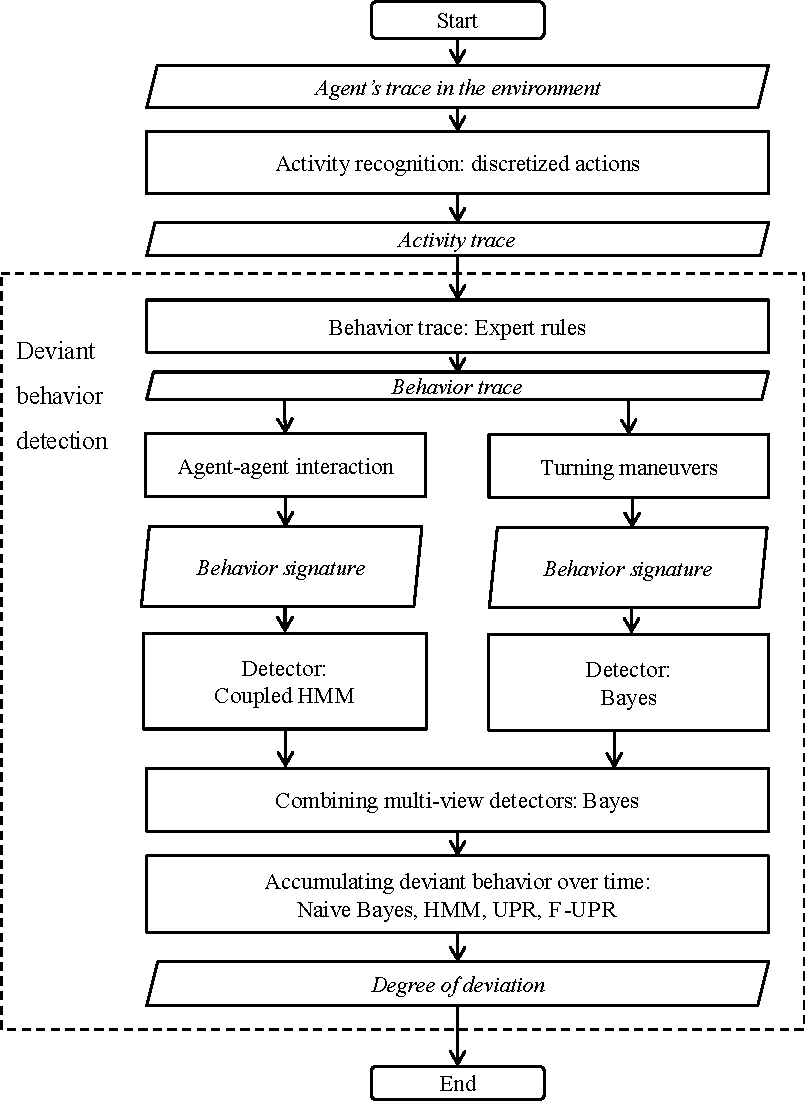
\includegraphics[width=0.8\linewidth]{chap_surveillance/stack-SURV.pdf}
\caption{Flowchart of the instantiated unified framework using two trigger event detectors and accumulating suspicious behavior.}
\label{fig:architecture-fupr}
\end{figure}


\subsection{Sensors and Observations}

The experiments in this chapter use ESCAPES~\citep{Tsai2011}, a state-of-the-art, multiagent airport evacuations simulator with several agent types exhibiting behaviors of regular travelers, authorities, and families. The agents' behavior incorporates emotional and informational interactions, such as emotional contagion, the spread of knowledge/fear, social comparison, etc. Therefore, an agent is affected other agents' emotional states, and is faced with uncertainty as to what happened and where the nearest exits are. We assume that the agent behavior corresponds to real airport passengers behavior.

ESCAPES consists of two parts: a two-dimensional environment based on the open-source project OpenSteer~\citep{opensteer}, outputting agents' physical trace coordinates; and a three-dimensional visualization component using the Massive Software~\citep{massive} to generate three-dimensional movies of the scenarios. We used a scenario that implemented the Tom Bradley International Terminal at Los Angeles International Airport, including terminals and shops as a realistic simulation environment. 

In addition to behaviors already modeled within ESCAPES, we introduced a suspicious behavior profile: an agent that behaved suspiciously prior an evacuation. Additional implementation details  are given in the experimetal section. An output example is shown in Figure~\ref{fig:airport:traces}, where traces of authorities (green), suspicious (red) and usual passengers (grey, blue) are plotted.
\begin{figure}[!ht]
\centering
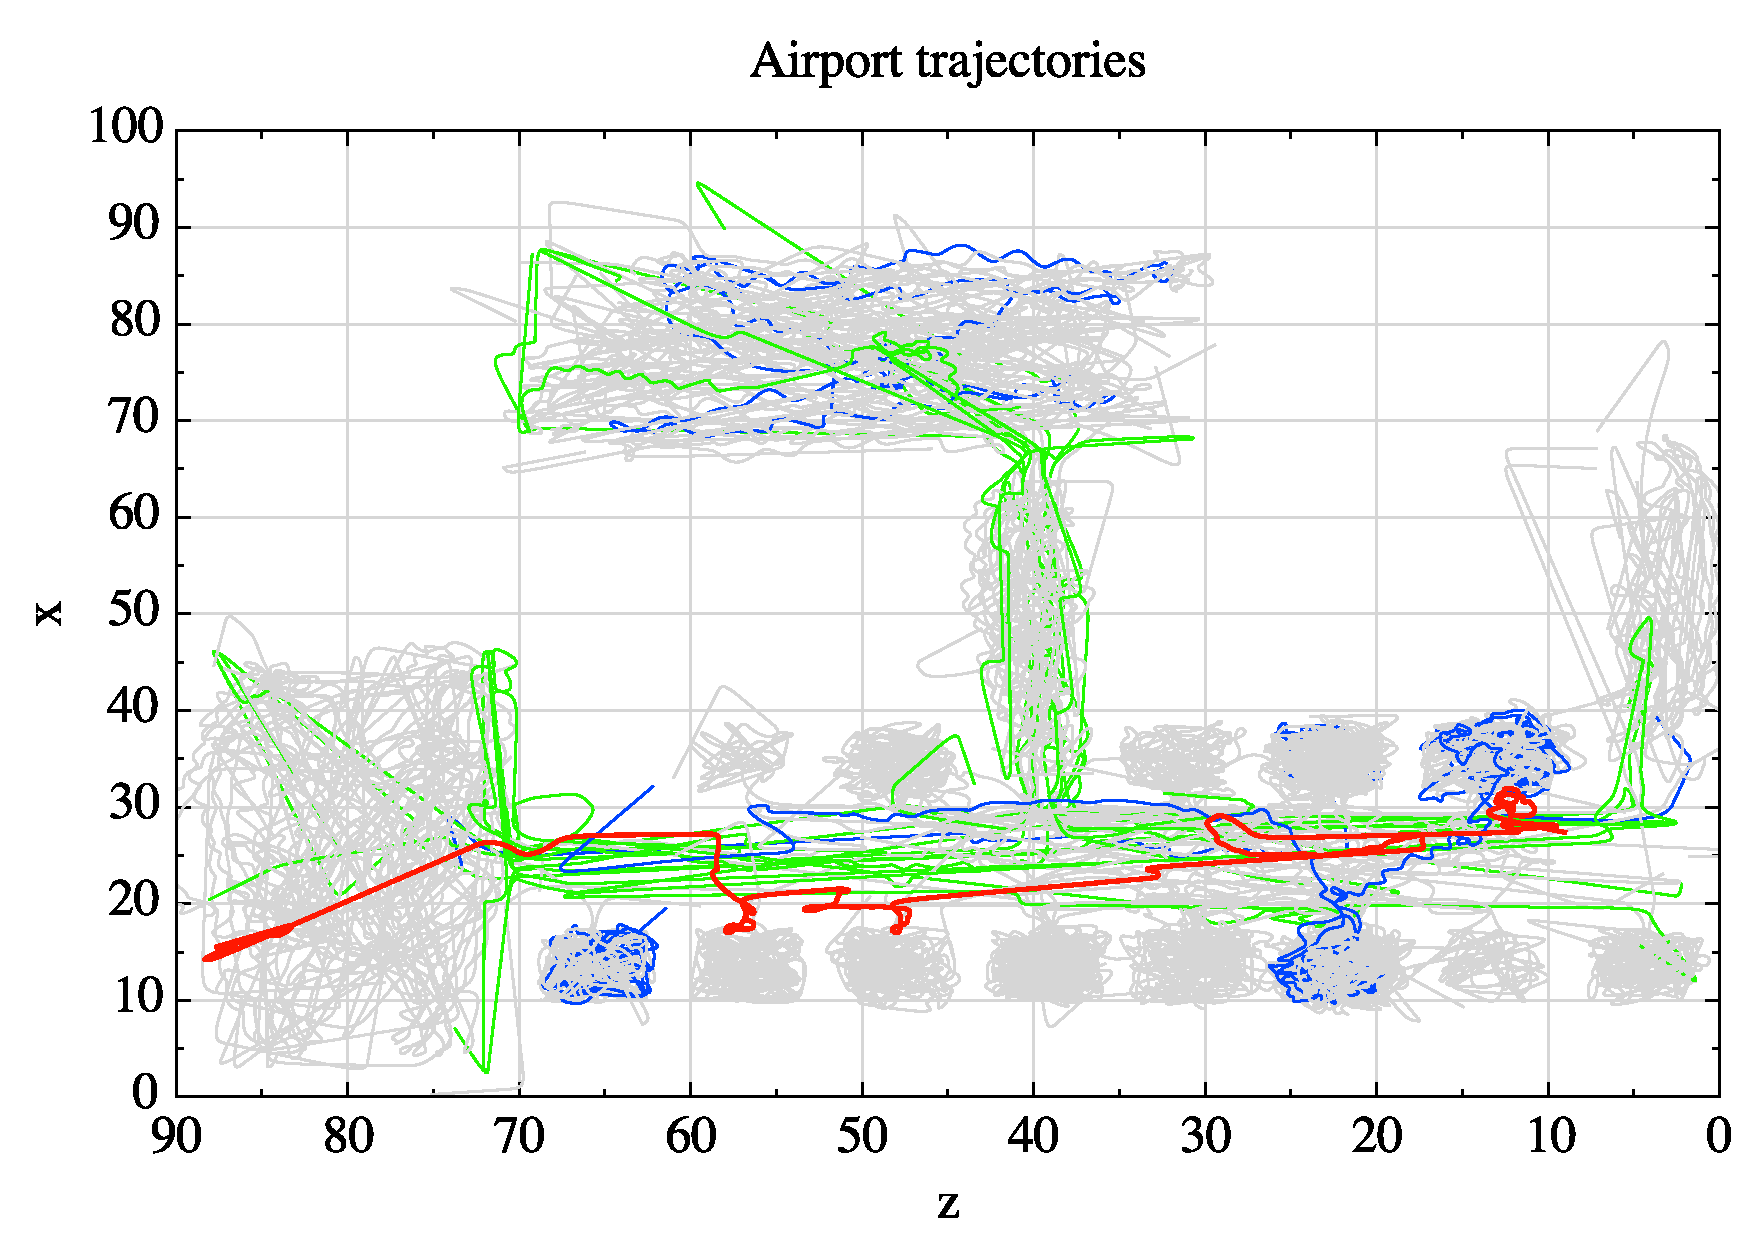
\includegraphics[width=0.95\linewidth]{chap_surveillance/airport}
\caption{Traces of all agents at the end of a simulation: authorities (green), suspicious (red), usual passengers (grey), and selected highlighted usual passengers (blue).}
\label{fig:airport:traces}
\end{figure}

An observation vector corresponds to absolute Cartesian coordinates at the airport map $\mathbf{x}_t=\tuple{x_t, y_t}$. Observation is then a sequence of vectors obtained during simulation; that is, $\mathbf{X} = \{\mathbf{x}_1, \dots, \mathbf{x}_T\}$.

%
%----------------------------------------------------------------------
%
\subsection{Atomic Activities}

%The trace of the coordinates was preprocessed to the action trace as follows. A change in position from the previous to the current state was described as taking the action of moving North, South, East and West, and their combinations (nine in total). This transformation describes the shape of a trajectory but discards the location information, which leads to better generalization. We also experimented with other transformations, for example, a more general one that also discards the orientation (forward, backward, left, right), and a less general one that divides the airport map with a square-based grid with numbered squares~\cite{Avrahami-Zilberbrand2009}. Preliminary tests showed the best performance when using the first transformation.

\index{activity recognition}
We considered three transformations of observation vectors to actions. The first divides the airport map  with a square-based grid into $N$ numbered squares~\citep{Avrahami-Zilberbrand2009}, which gives a set of possible atomic actions $\mathbb{A}_{fixed}=\{a_{s1}, \cdots, a_{sN}\}$.
Each observation sequence with Cartesian coordinates is transformed into a sequence of squares. We denote this as \emph{fixed representation}. By adjusting the square size, we can relax the model. By decreasing the square size, the model is more strict, less generalized, and may over-fit, since a too large size would cause over-generalization, that is, trajectories that are not similar might fit. %his presentation corresponds to approaches for detecting suspicious trajectories~\cite{Avrahami-Zilberbrand2009}.

The second representation, denoted as \emph{relative representation}, transforms Cartesian coordinates to actions taken in each time step as moving North, South, East, West and their combinations (nine in total); that is, 
$$\mathbb{A}_{rrep}=\{a_N, a_S, a_E, a_W, a_{NE}, a_{NW}, a_{SE}, a_{SW}, a_0\}.$$
Compared to fixed representation, relative representation also describes trajectory shape, but discards the location information, which leads to better generalization. 

The third representation, denoted as \emph{relative position and orientation}, defines actions as moving Forward, Backward, Left, Right and their combinations; that is, 
$$\mathbb{A}_{rrepor}=\{a_F, a_B, a_L, a_R, a_{FL}, a_{FR}, a_{BL}, a_{BR}, a_0\}.$$ Compared to relative representation, it also discards orientation information. 

%Preliminary tests showed 
Preliminary tests showed  the relative representation performed best \citep{Kaluza2011:PAIR}. The output of this level is an action sequence $\mathbf{a}=\{\mathbf{a}_1, \dots, \mathbf{a}_T\}$, where an action is assigned to each observation vector.


%The initialized system arch

%We address the problem of suspicious behavior detection in two steps, as shown in Figure~\ref{fig:architecture}. The first step analyzes an action trace and the surrounding environment to detect trigger events that characterize its interesting parts. The event trace then enters the second step, where it is evaluated. If the evaluation result exceeds a threshold value or is large relative to other evaluations of the event traces, then it is considered as suspicious.


%\subsection{Trigger Events}
%\label{sec:events}
%\noindent


%
%----------------------------------------------------------------------
%
\subsection{Compound Activities and Agent-Agent Interactions}

We focus on a well-known detector obtained from conversations with domain experts, and which is commonly used by behavior detection officers\footnote{An approach for monitoring passengers behavior over longer periods of time relies upon security personnel such as behavior detection officers (BDOs) that patrol airports to identify passengers who display \emph{involuntary physical and physiological actions}. US Transportation Security Administration (www.tsa.gov) trained and deployed BDO officers at over 160 US airports by 2011.}.
We observe the interactions between airport agents; more precisely, we are interested in how a passenger behaves in a uniformed authority figure's presence. A person exposed to a high level of stress produces behavior that indicates fear, anxiety, pressure, tension, deception, etc. Hence, it is rational for the suspicious agent to minimize contact with the authorities. Note, that no single avoidance is enough to raise a flag, but many such events taken together label the person as suspicious. 

We consider two types of trigger events or compound activities: interactions with authorities $\mathbb{I}=\{pass, avoid\}$, and changes of direction $\mathbb{B}=\{turn, no\_turn\}$. The idea behind these two trigger event types is to detect the likelihood that a passenger is trying to avoid an authority figure and that the change of direction occurs in general.

Both types of compound activities are detected with basic rules. The change of direction is detected by a threshold value over a trajectory curvature, while the interaction is detected by a threshold value over the distance between an authority and a passenger. The output of this level is behavior trace, where a tuple consists of a compound activity (indicating activity) and corresponding action subsequence (indicating spatial information); that is, 
$\mathbf{b}=\{\tuple{b_1, \mathbf{a}_{b_1}}, \dots, \tuple{b_{T'}, \mathbf{a}_{b_{T'}}}\}$. Such tuple is denoted \emph{trigger event} $e$, hence $\mathbf{b}=\{e_1, \dots, e_{T'}\}$.

%
%----------------------------------------------------------------------
%
\subsection{Suspicious Behavior Evaluation}

Behavior evaluation first evaluates each trigger event and estimates the likelihood that it was generated by a legitimate or a suspicious passenger, then combines the evaluations as shown in Chapter~\ref{chap:accumulation}.

The probabilities for each type of the trigger events are estimated separately. The turn event uses a \emph{frequentist estimator}; that is, \emph{a-priori} probability that a turn is generated by a suspicious or legitimate passenger:
\begin{equation}
		\hat{n}(e_t) = \Prob\{y=0|b=\text{turn}\},
\label{eq:freq-n}
\end{equation}
\begin{equation}
		\hat{s}(e_t) = \Prob\{y=1|b=\text{turn}\}.
\label{eq:freq-n}
\end{equation}

Interaction probability estimation is implemented with coupled hidden Markov models (CHMMs, introduced in Section~\ref{sec:ar:interactions}).
% %This results in a set of partial observations describing interactive behavior of a passenger. The recognition process first extracts all interactions between passengers and authority figures inside a given radius, producing a set of trajectory pairs that are transformed to relative presentation. 
%
%A trigger-event detection able to identify interactive behavior may rely on coupled hidden Markov models (CHMMs), which are briefly described below. The reader is referred to~\cite{Brand} for details; the CHMMs are not the main contribution of the paper.
% %To differentiate between authority-regular and authority-suspicious interactions we present an approach based on coupled hidden Markov models (CHMM). 
% %
The observations are constructed from two action sequences, namely the agent of interest's action sequence and the  authority agent's action sequence when they are within some predefined radius. The CHMMs use two HMM chains, where the hidden states from one chain directly impact the hidden states from the other chain. 
%Figure~\ref{fig:CHMMs} illustrates the CHMM for a pair of action traces with length $l=3$. The current state $Q_t^A$ of agent $A$ is affected by both its previous state $Q_{t-1}^A$ and previous state $Q_{t-1}^B$ of the agent $B$ (similarly $Q_t^B$ is affected by $Q_{t-1}^B$ and $Q_{t-1}^A$). Each state $Q_i$ also impacts the corresponding observation state $Y_t$. 
For example, if the authority agent moves toward the suspicious agent, the next state of the latter takes this into account and produces an action for an avoidance maneuver. 
% %The joint distribution for a pair of traces of length $k$ can be obtained by unrolling the network until we have $k$ slices, and them multiplying together all of the conditional probability distributions. 


% \begin{figure}[!ht]
% \centering
% \includegraphics[bb=0 0 595 830, angle=-90, width=0.5\linewidth]{chap_surveillance/chmm.pdf}
% \caption{An example of CHMM for a pair of action traces with length $l=3$.}
% \label{fig:CHMMs}
% \end{figure}

\index{detector}
A regular passenger may not turn or do anything different in the presence of authorities, while a suspicious person will, although as described below, an observer may not be perfectly observable. Therefore, we create and train two CHMMs: $\hat{N}_I$ models authorities' and regular passengers' interactions, while $\hat{S}_I$ models authorities' and suspicious passengers' interactions. For a new event (that is, interaction) $e$, we compute the posterior probability that the event is generated with both models yielding 
\begin{equation}
		\hat{n}(e_t) = \Prob\{e|\hat{N}\},
\label{eq:freq-n}
\end{equation}
\begin{equation}
		\hat{s}(e_t) = \Prob\{e|\hat{S}\}.
\label{eq:freq-n}
\end{equation}
\noindent
We also experimented with more complex CHMM structures including other features such as relative speed and distance, but the results were comparable or even worse. 


The second step, which evaluates the trigger event sequence, uses one of the detectors introduced in Chapter~\ref{chap:accumulation}: na{\"i}ve Bayes, HMMs, UPR, and F-UPR detector.
% %As a trigger event we also extract all turns in absence of authority when the trajectory curvature exceeds a threshold value. Probabilities that a turn event was generated by suspicious $\hat{n}_T(x)$ or regular passenger $\hat{s}_T(x)$ is acquired with frequentist estimator from the learning set $D_l$.
% %
% %
% %The second architecture (Figure~\ref{fig:CHMM-3}) incorporates additional information in the form of a model of relative speed between two agents. This model directly impacts the states of both agents. The idea behind this architecture is to improve recognition results with an additional information.
% %
% %Note that for an interaction of length $T$ the architectures presented in Figure~\ref{fig:CHMMs} are unrolled to $T$ slices. %(similar as in Figure~\ref{fig:HMM-4}). 


% %\begin{figure}[!ht]
% %\centering
% %\subfigure[]{
% %\includegraphics[width=0.25\linewidth]{CHMM-2}
% %\label{fig:CHMM-2}
% %}
% %\subfigure[]{
% %\includegraphics[width=0.25\linewidth]{CHMM-3}
% %\label{fig:CHMM-3}
% %}
% %\caption{CHMM presented as 2-sliced DBN: (a) modeling actions of two agents and (b) modeling both actions and relative speed.}
% %\label{fig:CHMMs}
% %\end{figure}





%
%==========================================================================================
%
\section{Experimental Evaluation}
\label{sec:Experiments}
\noindent
In cooperation with security officials, we defined a scenario where a suspicious passenger goes from point $A$ to point $B$ while trying to avoid security personnel at the airport. One may argue that an adversary that plans to do something malicious would behave normally in the presence of authorities, and this might be true for a highly trained individual. As discussed previously, an average person exposed to a high level of stress exhibits fear, anxiety, and tension, and, hence, tries to cover it by minimizing close-range interactions by making U-turns, avoidance maneuvers, hiding in nearby shops, etc. The agent behavior implementation details within ESCAPES are provided in Appendix B.

A simulation in ESCAPES is run with a given airport map, authority agents, regular passengers, and a suspicious agent going from point $A$ to point $B$, outputting traces with 2D coordinates for all agents. 
%An example is visualized in Figure~\ref{fig:airport:traces}, where the trace of the suspicious agent is marked with red (going from left to right), traces of authorities are green and regular passengers are blue and gray.
We initialized the simulator with $100$ agents, including $K_a \in \{5,10,15,20,25\}$ authorities and a suspicious person with randomly chosen initial and final points. For each $K_a$ setting, we ran $30$ simulations, each consisting of 1,500--3,000 time steps and $100$ traces. On average, there were $215$ interactions between the authorities and the passengers per run. 
%
To avoid issues that can arise with highly unbalanced datasets, we used random re-sampling without replacement to balance the data to the ratio \textit{suspicious : normal $=20:80$}. %From the original dataset we randomly selected ${}^2/_3$ of the suspicious examples representing $20\%$ of the new dataset, and then randomly selected the matching $80\%$ from the normal examples. For each configuration we repeated the random resampling ten times and averaged the results.
For the evaluation, we used \emph{precision}, \emph{recall}, \emph{specificity} and \emph{F-measure}. 
%Precision is defined as the number of true positives (all suspicious cases correctly classified as suspicious) divided by the number of all cases marked as suspicious (true and false positives): $pr=TP/(TP+FP)$. A perfect score $1$ means that all cases marked as suspicious were indeed suspicious. Hence, the score $1-pr$ represents the rate of \emph{false alarms}. Recall is defined as the number of true positives divided by the number of all the suspicious cases: $re=TP/(TP+FN)$. A perfect score $1$ means that all the suspicious cases were detected (but says nothing about falsely marked normal cases). Similarly, the specificity is defined for normal cases $sp=TN/(TN+FP)$. There are two points of interest, depending on our objective. The first one is when both scores are minimized; that is, the trade-off point between false alarms and non-detected suspicious passengers, which can be detected with the F-measure $FM=2 \cdot pr \cdot re/(pr+re)$. The other case is when a high false-alarm rate is acceptable and non-detected cases are extremely costly. In this case we are interested in precision when recall $re=1$; that is, all the suspicious passengers are found. In the worst-case scenario, all the passengers are marked as suspicious. 
We evaluate the statistical significance of our results using the two-sample $t$-test.








\begin{figure}[!ht]
	\centering
	\subfloat[$\exists k$ rule]{\label{fig:results:rule}
		\includegraphics[width=0.45\linewidth]{chap_surveillance/k-rule}}
	\subfloat[Naive Bayes]{\label{fig:results:bayes}
		\includegraphics[width=0.45\linewidth]{chap_surveillance/bayes}}

	\subfloat[HMMs]{\label{fig:results:hmm}
		\includegraphics[width=0.45\linewidth]{chap_surveillance/hmm}}
	\subfloat[UPR]{\label{fig:results:upr}
		\includegraphics[width=0.45\linewidth]{chap_surveillance/upr}}

	\subfloat[F-UPR]{\label{fig:results:fupr}
		\includegraphics[width=0.45\linewidth]{chap_surveillance/espy}}

\caption{Confusion error rates for different threshold values.}
\label{fig:results}
\end{figure}






%In our case we have a two-class problem; a trace can be classified as generated either by suspicious or normal passenger. 





%TODO: comment this approach ...
%\\...
%\\...

%\subsection{Detection Based on Multiagent\\ Interactions}
%\label{sec:2Layers}
%This section compares approaches based on a two-level architecture. The first level detects trigger events, while the second level takes a trace of events and decides whether it was generated by suspicious agent. We first present the detection of trigger events based on Coupled HMMs and trajectory curvature, and then compare the discussed approaches at the second level.




%\subsubsection{Results}



%\noindent
In the first experiment, we fixed the number of authority figures $K_a=10$. We instantiated the na{\"i}ve Bayes, HMMs, UPR, and F-UPR detectors. Additionally, we considered another baseline detector using a simple rule over the threshold $k$ and the event trace $\evec{t}$, saying that if the number of suspicious events exceeds $k$ (that is, $\exists k: \eta_s(\evec{t}) > k$), then mark trace $\evec{t}$ as suspicious.
%The input to the detectors is an event trace produced by the previous level. We instantiated Naive Bayes, HMMs, UPR, and Scoring function detectors. Additionally, we consider another baseline detector using a simple rule saying that if a trace $\mathbf{x}$ contains more than $k$ events most likely generated by a suspicious passenger, then classify it a suspicious. 
%
All the detectors used the event-trace probabilities $s'(\evec{t})$ and $n'=1-s'(\evec{t})$ as returned by the event-detection step. For the HMM approach, we considered two ergodic HMMs as described in Section~\ref{sec:HMMexp}. We used two observations, the normal $\Delta(e_t)=0$ and the suspicious $\Delta(e_t)=1$ event, and varied the hidden state number. The best results were achieved with three hidden states. Note that the HMM detector applied on top of the CHMM detector basically presents a version of the mixed- layer HMM structure~\citep{Fine1998, Nguyen2005, Duong2005}. All the models, including UPR and F-UPR detectors, were evaluated with 10-fold-cross validation. %We evaluated the statistical significance of our results using two-sample $t$-test. 

Figures~\ref{fig:results}(a)--\ref{fig:results}(e) show the confusion error rates for suspicious (1-\emph{recall}) and normal (1-\emph{specificity}) passengers as a function of the normalized threshold value for all the five algorithms. For example, if the threshold is zero, then all the passengers are marked as suspicious. In this case, all the suspicious passengers are correctly identified as suspicious; hence the error rate is also zero. Also, all the normal passengers are incorrectly identified as suspicious; hence the error rate is 1. As the threshold value increases, the error rate for correctly identifying suspicious passengers increases, while the error rate for correctly identifying normal passengers decreases.

There are two points of interest: (i) when the error rates cross each other; that is, the \emph{F-measure} is maximized; and (ii) the right-most point when the error rate for suspicious passengers is zero; that is, \emph{recall}$=1$ and the false-positive rate is minimized. These cases are tabulated in Table~\ref{tab:fmeasure}. The first case is summarized in columns 2--4 showing the  recall, precision and F-measure. F-UPR outperforms the $\exists k$ rule ($p<0.01$), na{\"i}ve Bayes ($p<0.01$), HMMs ($p<0.01$), and UPR ($p<0.01$). 
{The second case, where the threshold value is such that all the suspicious passengers are discovered, is shown in columns 5 and 6. Column 5 shows the confusion error for normal passengers (that is, 1-\emph{specificity}), while column 6 shows the ratio of correctly raised alarms (that is, \emph{precision}). The $\exists k$ rule, for instance, marks all the passengers as suspicious (FP rate is $100\%$) and consequently almost $80\%$ of alarms are false. HMMs achieve better performance, but still mark more than $50\%$ of normal passengers as suspicious. Other methods mark between 1/5 and 1/4 of normal passengers as suspicious, but precision is around $50\%$, which means that every second passenger marked as suspicious is indeed suspicious (and all suspicious passengers are discovered!). Overall, F-UPR in this setting outperforms the $\exists k$ rule ($p<0.01$), na{\"i}ve Bayes ($p<0.05$), HMMs ($p<0.01$), and UPR ($p<0.05$).
Finally, Figure~\ref{fig:ROC} depicts the ROC curves showing that F-UPR performs the same, or better, in all the threshold settings. 

\begin{figure}[!ht]
\centering
\includegraphics[width=0.8\linewidth]{chap_surveillance/ROC}
\caption{ROC curves comparing all the detectors.}
\label{fig:ROC}
\end{figure}

\begin{table}
\centering
\caption{Evaluation results when the F-measure is maximized (columns 2--4) and all the suspicious cases are discovered (the last two columns).}
\renewcommand{\arraystretch}{1.2}
\begin{tabular}{c|ccc|cc}
	\hline
						&	\multicolumn{3}{c|}{maximized F-measure}		&	\multicolumn{2}{c}{$recall$=1}		\\
	\hline
		Algorithm					& $re$	& $pr$	& $FM$		& $1-spec$		& $pr$\\		
	\hline
	$\exists k$ rule		& 0.619		& 0.464		& 0.530		& 1.000		& 0.202		\\		
	Naive Bayes				& 0.857		& 0.581		& 0.693		& 0.270		& 0.436		\\
	HMMs						& 0.600		& 0.706		& 0.649		& 0.526		& 0.286		\\
	UPR						& 0.857		& 0.720		& 0.783		& 0.256		& 0.477		\\
	F-UPR						& 0.905		& 0.905		& 0.905		& 0.217		& 0.539		\\
	\hline
\end{tabular}
\label{tab:fmeasure}
\end{table}

%\begin{table}
%\centering
%\caption{False positive and false negative rate when all suspicious cases are discovered ($re=1$).}
%\renewcommand{\arraystretch}{1.2}
%\begin{tabular}{c|c|c}
%	\hline
%		Algorithm			&FP rate ($1 - spec$)	 & Precision\\		
%	\hline
%	$\exists k$ rule		& 1.000		&0.202		\\		
%	Naive Bayes				& 0.270		&0.436 		\\
%	HMMs						& 0.526		&0.286	\\
%	UPR						& 0.256		&0.477	\\
%	F-UPR						& 0.217		&0.539	\\
%	\hline
%\end{tabular}
%\label{tab:getall}
%\end{table}


\begin{figure}[!ht]
\centering
\subfloat[F-measure is maximized.]{
\includegraphics[width=0.6\linewidth]{chap_surveillance/authvar-fm}
\label{fig:authvar:fmeasure}
}

\subfloat[All suspicious passengers are discovered.]{
\includegraphics[width=0.6\linewidth]{chap_surveillance/authvar-pr}
\label{fig:authvar:precision}
}
\caption{Evaluation results for varying the authority figure number in the simulation and two different threshold values.}
\label{fig:authvar}
\end{figure}

In the last experiment, we varied the number of simulated authorities. We expected that increased authority figures will result in more interactions with suspicious passengers, making detection easier. Figure~\ref{fig:authvar} shows the results for the $K_a \in \{5,10,15,20,25\}$ authority figures in a simulation:  Figure~\ref{fig:authvar:fmeasure} shows the F-measure for a maximizing threshold, while Figure~\ref{fig:authvar:precision} shows the precision when $\text{recall}=1$. Increased authority figures significantly increases detection capabilities. For example, the F-measure for F-UPR increases by $15\%$ when the security resources are doubled from five to ten, but as the number increases, the impact is smaller. We can also see that F-UPR achieves the same performance as other methods using significantly fewer security resources. 
%



\subsection{Detection Based on the Action Sequence}
\label{sec:HMMexp}
\noindent
We also applied a sanity check and tested the suspicious behavior detection from a sequence of agent actions (that is, action sequence $\mathbf{a}$) instead of a sequence of trigger events (that is, event trace $\mathbf{e}$). We used HMMs, since they are considered a baseline for modeling action sequences. The goal is to differentiate between a sequence produced by a suspicious and by a regular passenger. We expect this approach to perform poorly, since it is too general to precisely model interactive behavior present in a multiagent environment.

The suspicious behavior detector consists of two ergodic HMMs: $S'$ trained on the suspicious traces and $N'$ trained on the regular action traces. A new trace is first transformed to the action trace $\avec{k}$ as previously described and then matched against both HMMs, yielding the likelihood that it produced the given $\avec{k}$. If the likelihood is greater than a threshold, the action trace is marked as suspicious. 
%
%, and normal otherwise.%a behavior produced by the most probable model.%: $argmax(H_s(r), H_n(r))$.
%$$\frac{\lambda' \Prob\{ \avec{k}|S'\}}{(\lambda'}\Prob\{ \avec{k}|S'\} + (1-\check{\lambda})\Prob\{ \mathbf{x}|\check{N}\})} > \check{\tau},$$
%We run the experiments on We experimented with different number of hidden states and the best results are summarized in Table~\ref{}.
%We first report the results of running single-level HMMs with three different state presentations. 
%Table~\ref{tab:HMMresults} shows recall, precision and F-measure for trajectories presented with absolute position (column 2), relative position (column 3), and relative position and orientation (column 4). The second row shows results with acceptable discovery rate (recall), but extremely low precision around $10\%$ in the third row. This means that only $1$ out of $10$ passengers marked as suspicious was indeed suspicious. States presented with relative position outperform presentations with absolute position, which was expected. Absolute position requires a large data set to cover the complete state space, and second, it is prone to over-fitting. The presentations with relative position and orientation achieved lower recall than other presentations and slightly better precision. The reason can be in over-generalization. However, states represented with relative position were used in further experiments. 
%
We tested this approach for $K_a=10$ authorities. At the threshold value such that the highest F-measure 18.01 was achieved, this approach achieved an acceptable discovery rate ($\text{recall}=66.23$) and an extremely low precision (10.42). Such a performance positions this approach under the $\exists k$ rule.  The overall performance was consistent with our expectation that modeling single-agent actions in a multiagent environment would not capture the interactive behavior. 

%\begin{table}
%\centering
%\caption{Evaluation results for HMMs applied to the whole sequence of 2D coordinates presented as actions.}
%\renewcommand{\arraystretch}{1.2}
%\begin{tabular}{c|ccc}
%	\hline
%		[\%]		& Abs. pos.	& Rel. pos.	& Rel. pos.\&ori.\\		
%	\hline
%	Recall		& 62.63		& 66.23		& 40.86 		\\		
%	Precision	& 7.04		& 10.42		& 11.54 		\\
%	F-measure	& 13.24		& 18.01		& 18.00 		\\
%	\hline
%\end{tabular}
%\label{tab:HMMresults}
%\end{table}




\section{Identifying a Dangerous Driver}
\noindent
In addition to the airport domain, we applied UPR and F-UPR to the dangerous-driver domain, as introduced in \cite{Avrahami-Zilberbrand2009}. This domain also includes behavior that becomes increasingly costly if repeated: a driver switching a lane once or twice is not necessarily acting suspiciously, but a driver zigzagging across two lanes is dangerous. Our goal was to detect such drivers as soon as possible. 
%An example shown in Figure~\ref{fig:driver} depicts two lanes divided by a gird. There are two straight trajectories and one zigzag trajectory from left to right lane. 
%From each position, the driver can move horizontally to the next cell in the row, or to one of the diagonal cells.  A car in the left lane may be mistakenly observed (with small probability) to be in the right lane, and vice versa.

%\begin{figure}[h]
%\centering
%\includegraphics[width=0.7\textwidth, bb=0 0 1170 355]{lanes.pdf}
%\caption{Simulated trajectories for drivers~\cite{Avrahami-Zilberbrand2009}.}
%\label{fig:driver}
%\end{figure}

We generated 100 zigzagging driver observation sequences, each consisting of N observations, and 1,000 safe driver sequences. The trajectory observations were sampled with 10\% noise. If the driver stayed on the same lane as in the previous sample, the event was considered normal; otherwise, it was considered dangerous. For each sequence of trigger events, we accumulated the associated cost using both UPR and F-UPR. 
%Depending on a chosen threshold value, a driver may be declared dangerous if its accumulated cost is greater than the threshold, and safe if its accumulated cost is smaller than the threshold. 
Due to observation noise, the task is expected to be more difficult when less observations are available. As the number of available observations increases, it should be easier to distinguish between safe and dangerous drivers.


Table~\ref{tab:zigzag} reports the performance at the peak F-measure for different observation sequence lengths. The results confirm the airport domain experiments for two points. First, F-UPR performs better than UPR for any selected sequence length. Second, the performance of both methods increases as the number of observations increases, where F-UPR requires fewer observations than UPR to achieve the same performance. 
%Figure~\ref{fig:error} shows the confusion error rates at $N=75$, while Figure~\ref{fig:roc} compares ROC curves at the same observation sequence length. Figures for other $N$ values are quite similar and hence omitted.


\begin{table}[]
\centering
\caption{Evaluation results at the peak F-measure in the dangerous driver domain.}
\begin{tabular}{ccc}
\toprule
	Sequence length $N$ & F-UPR & UPR	\\
	\hline
	25 	&	0.632	&	0.540	\\
	50 	&	0.720	&	0.667	\\
	75 	&	0.900	&	0.800	\\
	100 &	0.952	&	0.857	\\
	125 &	1.000	&	0.947	\\
\toprule
\end{tabular}
\label{tab:zigzag}
\end{table}


\section{Conclusion}
\label{sec:Conclusion}
\noindent
This chapter instantiated the unified detection framework to successfully address the problem of suspicious behavior detection from a set of observations, where no single observation suffices to make the decision. The chapter addressed the problem in two steps; that is, the trigger event detection and a combination of evidence to reach a final conclusion. The proposed F-UPR approach was compared to competing approaches with comprehensive experiments on two simulated domains.
%a simulated airport domain. 
%By providing a new algorithm that outperforms other approaches, this paper has advanced the state of the art.




%We have modeled a trace of multiple trigger events as a mixture of two stochastic processes, normal and suspicious. We have defined detection of suspicious behavior as identifying those traces generated by the suspicious process. We have shown that optimal detection must take into account the complete history in the trace, which present a challenge in real-world applications. We discuss approaches that simplify detection by estimating conditional probabilities as well as approaches that relay on other frameworks such as plan recognition. We proposed a heuristic approach based on a family of \emph{well-behaved} scoring functions that interpret event to produce a score presenting overall suspicion that the trace corresponds to behavior of the suspicious agent using the complete behavior of the agent in the past. The approach was compared on the airport domain against both trajectory-based detection using HMMs and event-based detection using CHMM for detecting events and Naive Bayes, HMMs, UPR, and rule baseline for evaluating event traces. All of them were outperformed by the proposed approach.

%Verification procedure\\
% - evaluation on motivating domain -- airport scenario\\
% - proposes event detection procedure\\
% - compare different approaches using simulation
%Experimental evaluation on the airport domain first proposes an approach for detecting trigger events and then compares discussed approaches for evaluating whether an event trace is generated by normal or suspicious agent against the heuristic approach. The experiments in simulated multiagent environment show that the proposed approach outperforms other discussed solutions.


%TODO: UPDATE \emph{The paper presented EPSY, an event-based keyhole detector of suspicious behavior based on evaluating multiple partial observations by incorporating four key features: (i) dealing with infrequent partial observations; (ii) incorporating uncertainty arising from keyhole approach; (iii) forgetting mechanism; and (iv) adaptive reward and penalty functions. The approach was demonstrated on a motivating domain showing that ESPY is significantly better than basic, single-layered HMMs and two-layered HLHMMs, and comparable to the UPR approach. However, the ESPY showed that it can provide a viable solution for the detection of suspicious behavior by evaluating partial observations. It should be noted that the originality of this approach is inherent in the adaptive evaluation of multiple partial observations related to the behavior of an agent in the past. 
%
%An interesting perspective for the enrichment of the ESPY consists in active detection of erratic behavior by intentionally provoking responses from an agent for which there is either unclear or not enough information to draw the conclusion.}

With automatic behavior surveillance is it possible to identify passengers showing suspicious behavior that currently remains unnoticed. However, there are still shortcomings that are hard to bypass. For instance, observers can perceive whether someone appears anxious or is acting deceptively, they cannot tell whether that person is planning an attack or an extramarital affair. Although the \emph{intelligent behavioral surveillance} presents an important leap in security, it raises several privacy violation concerns, which should be addressed before deploying such systems in practice.



%In many cases, the extra scrutiny is a casual conversation with a TSA behavior officer that shows someone is innocent, 

%"behavioral surveillance" has "enormous potential for violating" privacy.

%"The shortcoming is, we don't know how many people are showing suspicious behaviors and aren't being noticed," Ekman said.

%Although observers can perceive whether someone appears anxious or is acting deceptively, they can't tell whether that person is planning an attack or something such as an extramarital affair, Levenson said.

%Our goal is to monitor a passenger 

%Airport security has increased drastically in recent years.
%Nowadays the security at the airports 
%Motivation...


%ACKNOWLEDGMENTS are optional
%\section{Acknowledgments}
%The authors would like to thank Zhengyu Yin for valuable discussion and suggestions, and Jason Tsai and Matthew Brown for their help with implementation challenges in the ESCAPES simulator. The work of Bo{\v s}tjan Kalu{\v z}a was supported partly by the Slovene Human Resources Development and Scholarship Fund and partly by the Slovenian Research Agency.

\newpage \thispagestyle{empty}

%!TEX root = thesis.tex


%
%==========================================================================================
%
\chapter{Security Domain}
\label{chap:civabis}

% \includepdf[pages=2-last, fitpaper=true, addtotoc={
% 2, section, 1, {A Probabilitic Risk Analysis for Multimodal Entry Control}, sec:eswa, %
% 2, subsection, 2, {Introduction}, sec:eswa:intro, %
% 3, subsection, 2, {Related Work}, sec:eswa:related, %
% 3, subsection, 2, {Hierarchical Multimodal Framework}, sec:eswa:framework, %
% 	3, subsubsection, 3, {Functional Description}, sec:eswa:framework:desc, %
% 	4, subsubsection, 3, {Architecture}, sec:eswa:framework:architecture, %
% 	4, subsubsection, 3, {Observing the person's behavior}, sec:eswa:framework:observing, %
% 	4, subsubsection, 3, {Experimental Environment}, sec:eswa:framework:environment, %
% 	5, subsubsection, 3, {Ontology}, sec:eswa:framework:ontology, %
% 5, subsection, 2, {Modules and Algorithms}, sec:eswa:modules, %
% 	5, subsubsection, 3, {Expert Rules}, sec:eswa:modules:rules, %
% 	6, subsubsection, 3, {Micro Learning}, sec:eswa:modules:micro, %
% 	6, subsubsection, 3, {Macro Learning and Meta-Learning}, sec:eswa:modules:macro, %
% 	7, subsubsection, 3, {Visual Learning}, sec:eswa:modules:visual, %
% 	7, subsubsection, 3, {Integration}, sec:eswa:modules:integration, %
% 8, subsection, 2, {Experimental Results}, sec:eswa:experiments, %
% 	8, subsubsection, 3, {Learning Phase}, sec:eswa:experiments:learning, %
% 	8, subsubsection, 3, {Evaluation Phase}, sec:eswa:experiments:evaluation, %
% 9, subsection, 2, {Discussion and Conclusion}, sec:eswa:conclusion, %
% 9, subsection, 2, {References}, sec:eswa:references %
% }]{article/ESWA5529.pdf}

Entry control is an important security measure that prevents undesired persons from entering secure areas. The unified detection framework utilized in this chapter allows an advanced risk analysis to distinguish between acceptable and unacceptable entries, based on several entry sensors, such as fingerprint readers, and intelligent methods that learn behavior from previous entries. First, it analyzes person behavior from different viewpoints and then performs a joint risk analysis. The obtained results represent an improvement in detecting security attacks.

%%%%%%%%%%%%%%%%%%%%%%%%%%%%%%%%%%%%%%%%%%%%%%%%%%%%%%%%%%%%%%%%%%%%%%%
%
% I N T R O D U C T I O N
%
%%%%%%%%%%%%%%%%%%%%%%%%%%%%%%%%%%%%%%%%%%%%%%%%%%%%%%%%%%%%%%%%%%%%%%%

\section{Introduction and Background}

Building and system safety and integrity have become more important due to the increased threat of terrorist attacks, system intrusions, and frauds. An important security requirement is to ensure effective entry controls that prevent unauthorized persons from accessing specific areas. 

The general approach is to combine a two-stage security check: the identification stage, where the person introduces his/her identity; and the verification stage, based on a password and/or one or more signals derived from physical traits, such as fingerprint, voice, iris or written signature. Although widely used, entry control has certain weaknesses in the real world. Classic security methods fail to recognize unauthorized access if, for example, an identification card is stolen, a fingerprint is faked, or an employee is forced to open the door for unauthorized persons. 
%Furthermore, a human supervisor or guard is not able to effectively control a variety of access points for several hours and can be fooled even by simple tricks.
However, intelligent access-control systems offer the promise of improved performance at a reasonable cost.

A common practice in most reported studies is to improve the two-stage security by (i) using advanced biometric methods \citep{Wahyudi2007, Wong2009, Sun2008}; (ii) analyzing behavior \citep{Zhang2007, Lin2008, Quah2008, Alexandre1997, wilson2006, Stephen2005, Depren2005}; or (iii) combining multiple sensors into a single, reliable estimation \citep{lamborn2006, Bontempi2005, Fierrez-Aguilar2005}. In all the above-referenced studies, the methods successfully reduced the risk of intrusion, although each approach was focused on one specific viewpoint. \citet{Wahyudi2007}, for example, presented a verification based on speech analysis. They constructed voice-based models for authorized persons and performed the identification with an adaptive network-based fuzzy-inference system. In a similar way, \citet{Wong2009} and \citet{Sun2008} focused on face recognition. Various facial features were extracted from video, saved in a database and compared with a new entry. The authors report an accuracy of over 90\%.

Recent research efforts have focused on meta-learning \citep{Brazdil2009, Vilalta02, Wang1997}. The basic objective is to consider various aspects and hypotheses about an event and the environment to construct a situational awareness;  then, on this basis, risk is reliably estimated. \citet{lamborn2006} introduced an intelligent system that consists of several heterogeneous sensors divided into clusters according to their GPS location using self-organizing maps. Sensor outputs are classified into each cluster and a voting algorithm is used to compute the final classification. Several data-mining methods were tested for cluster classification; for example, k-NNs, neural networks, and SVMs. A similar system was presented by \citet{Bontempi2005}. In addition, \citet{Fierrez-Aguilar2005} exploited person-specific multimodal biometric parameters. They proposed an adapted local learning scheme (person-de\-pen\-dent) and global learning scheme (person-in\-de\-pendent), with both results fused with weighted voting. The authors reported that the adapted learning outperformed the results from single learning.


The described approaches use state-of-the-art methods that successfully reduce intrusion risk. They use additional biometric sensors and behavior analyses as upgrades to classic access control. Our approach is a further step in combining an arbitrary number of methods in three stages. In the first stage, an arbitrary number of intelligent modules is utilized, with analyzing person behavior from different viewpoints and performing its own risk analysis. Similar to \citet{lamborn2006}, our system constructs a situational awareness from different sensors, but, in contrast to their method, the intelligent module outputs in the second stage are assembled using meta-learning, on top of which the final reasoning is performed with a Bayesian network. In addition, the intelligent modules utilize both person-specific parameters and global knowledge similar to \citet{Fierrez-Aguilar2005}, but the last integration is fused proficiently. Finally, the system is also able to explain the evaluations to a human operator and helps him/her to understand the situation. The basic assumptions of our approach are that (i) person behavior rarely changes significantly over time, and (ii) combined methods are much harder to bypass than a single sensor or method.

%The rest of this chapter is structured as follows. Related work is described in detail in Section~\ref{sec:relatedWork}. The general structure of the proposed framework is presented in Section~\ref{sec:system}, while Section~\ref{sec:modules} describes the individual modules and the final integration in detail. Section~\ref{sec:results} presents the experimental evaluation and results with an on-line adversary test. Finally, Section~\ref{sec:conclusion} summarizes the work done and concludes the chapter with a discussion.


%%%%%%%%%%%%%%%%%%%%%%%%%%%%%%%%%%%%%%%%%%%%%%%%%%%%%%%%%%%%%%%%%%%%%%%
%
% R E L A T E D   W O R K
%
%%%%%%%%%%%%%%%%%%%%%%%%%%%%%%%%%%%%%%%%%%%%%%%%%%%%%%%%%%%%%%%%%%%%%%%


%%%%%%%%%%%%%%%%%%%%%%%%%%%%%%%%%%%%%%%%%%%%%%%%%%%%%%%%%%%%%%%%%%%%%%%
%
% S Y S T E M
%
%%%%%%%%%%%%%%%%%%%%%%%%%%%%%%%%%%%%%%%%%%%%%%%%%%%%%%%%%%%%%%%%%%%%%%%

\section{Hierarchal Multimodal Framework}
\label{sec:system}

%\subsection{Functional Description}
%\label{sec:system:description}

The aim of our system is to ensure increased security in critical areas, such as military headquarters or political institutions, by detecting irregular accesses or unusual access point behavior, and, on this basis, raising an alarm. In order to reduce intrusion risk, we have designed a modular system that relies heavily on intelligent methods.

\subsection{Functional Description}
\label{sec:system:description}

The entry procedure is shown in Figure~\ref{fig:procedure} and is as follows: first, a person is identified. Next, if his/her identity exists, the person is verified, which leads to the door lock being released. The verification process is performed in two stages: a classic biometric verification, and an intelligent verification. Intelligent modules evaluate the entry and suggest the proper action.

\begin{figure}[!ht]
\centering
\includegraphics[width=0.6\linewidth]{chap_security/entry}
%\includegraphics[bb=100 230 380 600, width=8cm]{chap_security/entry.pdf}
\caption{Entry identification and verification procedure at a high-secured access point.}
\label{fig:procedure}
\end{figure}

The proposed intelligent access-control system's development was based on the following five requirements: first, the system must monitor entries and process evaluations in real time. Second, several access points may need to be monitored at the same time, taking into account knowledge of the person's movement between them. Third, an arbitrary number of sensors and intelligent modules will be used, depending on the equipment at specific access points and data availability. Fourth, the system is expected to evaluate an entry and suggest the proper action. Finally, the system should explain its evaluation in a user-friendly, interactive control panel. In short, the aim is to create a system that will improve entry control security and help the operator to control numerous access points effectively. 


\subsection{Architecture}
\label{sec:system:architecture}

\index{unified framework}
The main architectural tasks are collecting the data from the peripheral devices and sensors, processing and analyzing this data, integrating the analyses into a human-readable form, and displaying them to a person with a suggestion for an appropriate action (Figure~\ref{fig:architecture}). 


\begin{figure}[!ht]
\centering
\includegraphics[width=1\linewidth]{chap_security/stack-SEC}
%\includegraphics[bb=80 410 470 780, width=8cm]{chap_security/architecture.pdf}
\caption{Flowchart of the instantiated unified framework using multiple time scales and modalities to evaluate behavior.}
\label{fig:architecture}
\end{figure}

% \begin{figure}[]
% \centering
% \includegraphics[width=0.8\linewidth]{chap_security/architecture}
% %\includegraphics[bb=80 410 470 780, width=8cm]{chap_security/architecture.pdf}
% \caption{General architecture of the system. Our contribution is in gray.}
% \label{fig:architecture}
% \end{figure}


The system's architecture is designed in eight layers. In the first layer, various access point sensors are deployed, such as biometric sensors, visual sensors, or door opened/closed sensors. The sensors' output is captured in the next layer through a controller, providing an observation vector $\mathbf{x}_t$ at time step $t$, augmented with additional contextual information.

\index{activity recognition}
The activity recognition layer is simplified to recognizing $\mathbb{A}=\{entry, other\}$. If all the formal criteria are met, that is, the observation consists of all the required elements, then the activity is marked as \textit{entry} and evaluated as shown in Figure~\ref{fig:procedure}; otherwise, the entry is not completed and an alarm is raised immediately.

The next three levels are implemented in several parallel instances. Each instance constructs its own behavior patterns from a specific data type, such as visual data or temporal relations,  and applies an intelligent method to evaluate the behavior. The methods include decision trees, outlier detection, expert rules, computer vision and others. Finally, all previous parallel detector outputs are gathered and the system outputs the final evaluation using a Bayesian network.


\subsection{Observing the User's Behavior}
\label{sec:system:behavior}

Each human tends to perform activities in a specific way, be it on micro-or macro-scale. However, the person behavior in our system is actually monitored from three different points of view. In the first of these, denoted as the \textit{micro-level}, one typically deals with behavior that changes in seconds or tenths of a second. For example, one person always carries his identity card in a wallet and puts the whole wallet near the wireless identity-card reader, while another person carries her card in a handbag and requires some time to take it out, identify herself, and put the card back. The person's movement around the access point depends on his/her habits and mental/physical state. These facts determine the persons' micro-level patterns.

The second viewpoint, denoted as the \textit{macro-level}, describes the persons' daily routines. The activities are the access point arrival times, the movements between various access points in the access-control network, and even the connections between persons; for example, person $A$ often enters a short time after person $B$. The time scale used at the macro-level can vary from seconds to months.

The third viewpoint, denoted as the \textit{visual level}, captures the persons' access point visual movement using a camera. It is also focused on micro-level movements; that is, behavior that changes over a short time interval. However,  in addition to micro-level features, it obtains visual characteristic features of the person and his/her movement; for example, the person's height and the door-opening dynamics.

Several rules additionally control the regular entry procedure, the regular working time, and access permissions.


\subsection{Experimental Environment}
\label{sec:system:experimental}

To design and test our intelligent access control modules, we set up the experimental environment shown in Figure~\ref{fig:environment}, which consisted of a single access point protecting an office in a building. The access point was equipped with a camera (on the ceiling), a card reader and a fingerprint reader (on the wall near the door), an electronic lock, and an open/close sensor on the door. The input signals were collected with a multi-channel access controller connected to various peripheral devices. 
%Such controllers can be dynamically combined in order to ensure the centralized data management of sensors covering a complete access-control network. However, for our purpose, one controller was sufficient.

\begin{figure}[!ht]
\centering
\includegraphics[width=0.8\linewidth]{chap_security/soba}
\caption{Prototype access-point configuration (camera view). The task is to detect suspicious entries of persons, for example, under the influence of drugs or with a gun that is outside the camera's field of view.}
\label{fig:environment}
\end{figure}

When a person passed the access point, four different times were registered:
\begin{itemize}
    \item	$t_c$ -- time of card-reader acceptance,
    \item	$t_f$ -- time of fingerprint-reader acceptance,
    \item	$t_{do}$ -- time of door opening,
    \item	$t_{dc}$ -- time of door closing.
\end{itemize}
The data was collected and written into the ontology for additional processing by six intelligent modules. The first module, denoted as the \textit{expert rules}, detected prohibited and basic undesired behavior. It used SWRL rules to query the system ontology (see Section~\ref{sec:modules:rules}). The second module, \textit{micro-learning}, learned person micro-level behavior patterns during the entry. The learning was performed with a local outlier-detection me\-thod (LOF) (described in more detail in Section~\ref{sec:modules:micro}). The three  \textit{macro-learning} modules learned the macro-level access patterns and were then combined at the meta-level (see Section~\ref{sec:modules:macro}). The last module, \textit{visual learning}, used optical flow histograms to detect visual-level behavior patterns (see Section~\ref{sec:modules:visual}).

Each module performed its own entry risk analysis and then returned an evaluation with an explanation. The meta-module used basic weighted voting based on single-module decisions, while the integration module accepted the module classifications as observations and performed the reasoning with a Bayesian network. 

\begin{figure}[]
\centering
%\includegraphics[bb=60 100 570 350, type=eps,ext=.eps,read=.eps,width=18cm]{chap_security/shema}
\includegraphics[width=0.95\textheight, angle=90]{chap_security/shema.pdf}
\caption{Information flow in the implemented platform.}
\label{fig:implementation}
\end{figure}
%\clearpage

Based on the final probability, the entry was classified into one of the classes: \textit{OK}, for regular entry, and \textit{alarm}, for irregular entry.
The system ontology stored each module's evaluations and explanations. The platform is presented in Figure~\ref{fig:implementation}. 
%It comprehends information flow from peripheral sensors through modules, up to the final integration and reports available to the human operator. 


\subsection{Ontology}
\label{sec:ontology}

The modules and methods use the same or similar data while processing, and therefore require a comprehensible presentation. Besides the basic relationships between pieces of information, such as the sensor's value, complex representations are also required; for example, a sensor \textit{belongs to} an access point.

We have developed an ontology using the Web Ontology Language (OWL) \citep{Horrocks03} and the ontology editor \cite{Protege}. 
The ontology consists of a central part, including event data and its classifications, and several local parts, each of them storing particular module knowledge. The central part includes information about: 
\begin{itemize}
    \item  	access points: position, security requirements etc; 
    \item 	persons: personal details, position in a company, rooms of the building that a person has permission to enter etc; 
    \item 	sensors: type; for example, biometric sensor, sensor access point;   
    \item 	events: person who produced the event, access point where it was produced, event sensors, individual module and final classification, and actions enabled via evaluation.
\end{itemize}

The ontology structure ensures knowledge of the system and its setting in a flexible presentation. This means that new sensors, modules, and access points can be easily added.





%%%%%%%%%%%%%%%%%%%%%%%%%%%%%%%%%%%%%%%%%%%%%%%%%%%%%%%%%%%%%%%%%%%%%%%
%
% M O D U L E S
%
%%%%%%%%%%%%%%%%%%%%%%%%%%%%%%%%%%%%%%%%%%%%%%%%%%%%%%%%%%%%%%%%%%%%%%%

\section{Detectors}
\label{sec:modules}

\index{detector}
This section describes the modules and algorithms in more detail. In this particular implementation, we prefer algorithms that can provide as much of an explanation as possible, but in general, it is possible to select any learning algorithm.


\subsection{Expert Rules Detector}
\label{sec:modules:rules}

The first module consists of expert rules defined by a security expert or a human operator. These rules do not learn from past person behavior; instead each rule has adjustable parameters, enabling new rule creation by specifying the rule-parameter values. 
The rules are described in the SWRL language \citep{W3Cswrl} for querying data stored in the OWL. A test over the events is performed by the Jess rule engine \citep{Jess}. 

We have implemented two types of rules. If the entry procedure is violated, the first rule type triggers an alarm independently of the other modules. The second rule type refers to the entry observation; for example, \textit{``The person accessed this area more than five times in the past two minutes''}. Instead of unconditionally triggering an alarm, each triggered rule $R_i$ returns a probability $\Prob\{R_i\}$ that the entry is regular. If several second-type rules $R_1, \dots, R_n$ are triggered, then $min(\Prob\{R_1\}, \dots, \Prob\{R_n\})$ is returned and the module composes an explanation consisting of the violated rules and their parameters. Otherwise, if none of the rules is violated, the entry is regular according to the rules, and, therefore, the returned probability $p$ equals $1$.

An example of the second-type SWRL rule is shown in Figure~\ref{fig:SWRL}.
\begin{figure}[]
\centering
\begin{verbatim}


event(?event_object) & swrl_end_of_testing(?event_object, ?event_swrl) &
swrlb:equal(?event_swrl, false) & card_time(?event_object, ?time_of_event) &
swrlb:greaterThan(?time_of_event,  "18:00:00") &
swrlb:lessThan(?time_of_event, "7:00:00")
THEN
swrl_rules_result(?event_object, "0.0") &
swrl_rules_explanation(?event_object, ?event_swrl_explanation) &
swrlb:stringConcat(?event_swrl_explanation, 
                   "Alarm: event time is between 18:00 and 7:00")
\end{verbatim}
\caption{An expert-rule example written in SWRL.}
\label{fig:SWRL}
\end{figure}
The rule queries events that occurred between 6:00pm and 7:00am and marks these events as alarms, since events are not allowed at night.



\subsection{Micro-Movement Detector}
\label{sec:modules:micro}

The micro-learning module learns short-term behavior. The attributes are calculated as three time differences from four input times:
\begin{eqnarray}
   \Delta t_1 &=& t_f-t_c, \\
    \Delta t_2 &=& t_{do}-t_f, \\
    \Delta t_3 &=& t_{dc}-t_{do}.
\end{eqnarray}
Each observation $\mathbf{x}_i$ is thus represented by a triple $\mathbf{x}_i=(\Delta t_{i,1},\Delta t_{i,2},\Delta t_{i,3})$. All the regular entries of a particular person form a learning set $\mathcal{X}=\{\mathbf{x}_1,\mathbf{x}_2,\dots ,\mathbf{x}_n\}$. When the person produces a new observation $\mathbf{x}_{n+k}$, the module compares it with the learning set $\mathcal{X}$ and returns an outlier factor: if the new observation is similar to the existing observations, $\mathbf{x}_{n+k}$ is a regular observation with a low outlier factor; otherwise, it is an outlier with a high outlier factor.

In previous work, \cite{Tusar2006} examined various outlier detection algorithms, selected the LOF (Local Outlier Factor, \citep{Breunig2001}) and implemented it. The algorithm reportedly achieves reliable performance where instances are not uniformly distributed in the attribute space. 
The LOF for a new observation $\mathbf{x}_i$ is defined as 
\begin{equation}
LOF_k (\mathbf{x}_i )=\frac{1}{|ngb_k (\mathbf{x}_i,\mathcal{X})|} * \sum_{\mathbf{y} \in ngb_k(\mathbf{x}_i,\mathcal{X})} \frac{ldns_k(\mathbf{y})}{ldns_k (\mathbf{x}_i)},
\end{equation}
where $ngb(\mathbf{x}_i,\mathcal{X})$ is the set of $k$-nearest neighbors of the observation $\mathbf{x}_i$, and $ldns_k(\mathbf{y})$ is the local density of an observation $\mathbf{y}$ and its $k$ nearest neighbors. Intuitively, $LOF_k (\mathbf{x}_i ) \leq 1$ when the new observation is near an existing cluster within $\mathcal{X}$, and $LOF_k (\mathbf{x}_i )  >1$ when the observation is far from the cluster.

The final outputs of the module are the LOF value, the probability that the entry is regular, and a visual explanation. The probability is computed from the LOF value using the following procedure. Let $\tau_l < 1$ denote the regular entry threshold value and let $\tau_u > 1$ denote the irregular entry threshold value. Then, the probability $\Prob\{\mathbf{x}\}$ that the entry $\mathbf{x}$ is regular is computed as a linear threshold values combination:
\begin{equation}
   p(e) =  \begin{cases} 
1.0 & \text{if } LOF(e) \leq \tau_l, \\
0.0 & \text{if } LOF(e) \geq \tau_u, \\
\frac{\tau_u-LOF(e)}{\tau_u-\tau_l} & \text{otherwise}.
\end{cases}
\end{equation}


%\frac{b_u-LOF}{b_u-b_l} \text{otherwise} \\

Since the module uses only three micro-attributes, its visualization can be presented in a three-dimensional space, with one dimension for each attribute. The entries are thus presented as points, and the each point's LOF value is represented by a color: red for outliers, yellow for unclear entries, and green for regular clustered entries. Figure~\ref{fig:microLOF} shows an entry cluster in a learning set $\mathcal{X}$ (circles) and a new entry $\mathbf{x}_i$ (a plus).


\begin{figure}[]
\centering
%\includegraphics[type=eps,ext=.eps,read=.eps,width=8cm]{chap_security/mikro1}
%\includegraphics[bb=45 75 375 270, width=8cm]{chap_security/mikro1}
\includegraphics[width=0.9\linewidth]{chap_security/mikro1}
\caption{Regular entries of a particular person (circles) and a new entry denoted as an outlier ('+').}
\label{fig:microLOF}
\end{figure}


\subsection{Macro-Movement and Meta-Detector}
\label{sec:modules:macro}

The macro-level data are used in three modules, two of which also exploit the micro-level data. The macro-level attributes are divided into two groups describing a current entry and the relation between the current entry and previous entries. The attributes from the first group are, for example, the current time and date, the day of the week, the date in relation to the month (that is, the second Friday in the month). The second group defines such relations as the number of previous entries in the same day (for the current person), the person who entered previously in a specific time interval, the entry time on the same day in the previous week, etc. 
It is important to note that macro-learning would be more powerful if we had monitored more than one access point.

The first macro-module learns only from macro-attributes. The positive learning examples are a person's regular entries, while the negative learning examples are a person's  irregular entries and the entries of other persons. Several machine-learning algorithms were tested and, finally, decision trees were selected,  Weka's J48 implementation of C4.5, in particular \citep{Witten2005}. The main decision tree benefit is the ability to explain a decision after classification. The path leading from the root to the chosen leaf is colored according to the classification: green for regular entries and red for alarms. Target variable distribution in the chosen leaf is interpreted as the probability that the entry is regular. The classification problem was introduced as a verification, where each person has his/her own decision tree with two possible outcomes: true, if the claimed identity is valid, and false otherwise.

The second macro-module applies the same algorithm as the previous module, but uses both micro- and macro-attributes. While the first macro-module considers only macro-level behavior and discovers patterns, for example, \textit{``User X comes to work on Mondays between 8.15 and 8.40~(93\%)''}, the second macro-module refines these patterns by incorporating micro-attributes.

\index{local outlier factor, LOF}
In the third macro-module, the macro- and micro-attributes are used for learning with the LOF algorithm. In contrast to the micro-module, where the visualization was intuitive, the large number of attributes requires a different representation. For this purpose, we implemented parallel coordinate visualization. Each attribute is presented on one vertical axis, ranging from the minimum to the maximum normalized value. Thus, each entry is represented as a broken line intersecting the attribute value coordinates. The line is colored according to the entry's LOF value: green for regular entries, yellow for unclear entries, and red otherwise. Figure~\ref{fig:macroLOF} shows a cluster of learning set entries and the new entry as a dotted line.

\begin{figure}[]
\centering
%\includegraphics[type=eps,ext=.eps,read=.eps,width=8cm]{chap_security/makro-lof}
%\includegraphics[bb=80 50 390 300,width=8cm]{chap_security/makro-lof}
\includegraphics[width=0.7\linewidth]{chap_security/makro-lof}
\caption{Multi-dimensional representation of regular entries (thin lines) and a new entry (dotted line) classified as an alarm. There are nine attributes with values normalized between the minimum and maximum values.}
\label{fig:macroLOF}
\end{figure}


Finally, the macro-meta-module combines the classifications of all three macro-modules. Then, all the results and visualizations are written into the ontology. %In the tested prototype, only weighted voting was implemented; however, several meta-level learning algorithms were applied later. 
Also, in the tested implementation, only the macro-meta-learning was applied, but in principle, an arbitrary subgroup of modules could be connected using meta-learners. 

\subsection{Visual Detector}
\label{sec:modules:visual}

The visual learning module developed by \cite{pers2007} learns person movement patterns using an access point video camera and classifies a new entry as either regular or not. For this purpose, a web camera with a $1.3$ Mpixel resolution and 30-fps rate was used.

When a new entry occurs, the last 30 seconds of video are analyzed in the following steps: first, the optical flow histograms are computed and divided into six segments, approximating body parts. Next, in each segment, the prevailing movement is estimated and transferred into a sequence of symbols. This sequence defines the movement's digital signature and is used for the verification. Each person has a learning set of valid regular entries, which are compared with the new entry signatures. Finally, the module outputs the classification and probability that the entry is regular as a normalized comparison. 

It should be noted that other sensor analyses, such as speech or walking patterns, could be added as well.

\subsection{Multimodal Detector Integration}
\label{sec:modules:integration} 
	
After the expert rules, micro-learning, macro-learning, meta-learning, and visual-learning have made their assessments, their results are integrated into a current entry joint risk analysis. It estimates the event probability $\Prob\{$\textit{entry $|$ entry is regular}$\}$ given the module observations. If the estimated probability does not exceed a threshold value, an alarm is triggered. Note that an alarm can also be triggered by expert rules when there is sufficient certainty.

The reasoning in the prototype system is performed with a Bayesian network, structured as shown in Figure~\ref{fig:bayesianNetwork}. Four modules have a direct impact on the entry event; that is, expert rules, micro-learning and visual learning, and a macro-meta-learning module, while the macro-meta-learning module depends only on the three macro-modules. The network probabilities are computed from the train dataset, using the \textit{m-estimate} for conditional probabilities and the \textit{Laplace estimate} for a-priori probabilities. 
\begin{figure}[]
\centering
\includegraphics[width=0.8\linewidth]{chap_security/BayesNetwork2}
%\includegraphics[bb=30 590 360 820,width=8cm]{chap_security/BayesNetwork.pdf}
%\includegraphics[bb=0 540 440 800,width=8cm]{chap_security/BayesNetwork2.pdf}
\caption{Bayesian network used for reasoning.}
\label{fig:bayesianNetwork}
\end{figure}

The integration proceeds in three steps. Firstly, the output from each module is converted to interval the $[0, 1]$ representing the a-posteriori probability $\Prob\{M_i\}$ that the entry event is regular. Secondly, given the Bayesian network and the probabilities $\Prob\{M_i\}$, the estimated  probability of an entry event is computed from the network.
%\begin{eqnarray}
%P(E | M_1, M_2, \dots, M_n) = P(E) \frac{P(M_1, M_2, \dots, M_n | E)}{P(M_1, M_2, \dots, M_n)}
%\end{eqnarray}
%Numerator is developed with chain rule and due to the structure of the network is simplified to:
%\begin{multline}
%P(M_1, M_2, \dots, M_n | E) = \prod_{i=1}^{n} P(M_i | Parents(M_i)) = \\
% = \prod_{i=1}^{n} p_{M_i} P(M_i=1|E) + (1-p_{M_i}) P(M_i=0|E)
%\end{multline}
%Denominator, on the other hand, is independent of the event E, thus is developed as follows:
%\begin{multline}
%P(M_1, M_2, \dots, M_n) = \\
% = \sum_{e\in\{0, 1\}} P(E=e) P(M_1, M_2, \dots, M_n | E=e)  =\\
% = \sum_{e\in\{0, 1\}} P(E=e) \prod_{i=1}^{n} (p_{M_i} P(M_i=1|E=e) + \\
% + (1-p_{M_i}) P(M_i=0|E=e))
%\end{multline}

Finally, the integration module outputs the joint analysis as a probability that the entry is regular and provides an explanation. According to the threshold values, the integration module triggers \textit{alarm} or \textit{OK} and stores the results in the ontology. In high-security areas, the cost of a false alarm is negligible compared to the cost of an unrecognized intruder; therefore, the system is set to minimize the latter.



%%%%%%%%%%%%%%%%%%%%%%%%%%%%%%%%%%%%%%%%%%%%%%%%%%%%%%%%%%%%%%%%%%%%%%%
%
% E X P E R I M E N T A L   R E S U L T S
%
%%%%%%%%%%%%%%%%%%%%%%%%%%%%%%%%%%%%%%%%%%%%%%%%%%%%%%%%%%%%%%%%%%%%%%%

\section{Experimental Results}
\label{sec:results}
  



An experimental verification was performed in the prototype environment as described in Section~\ref{sec:system:experimental}. It consisted of learning and evaluation phases. In this chapter, we report on one learning and three evaluation experiments.

\subsection{Learning Phase}
In the learning phase, four people were recorded accessing the system. Each individual completed 40 regular entries that were used as positive learning examples. The negative learning examples for one individual were the entries of the other three people. We built decision trees for the macro-modules, constructed learning sets for the LOF algorithm in the micro-and macro-module and a comparison set for the visual learning module, and adjusted the system parameters. After the learning was completed, the system was ready to operate. 


\subsection{Evaluation Phase}
In the evaluation phase, we performed three experiments: two with simulated entries and one real-time experiment with security experts. 

The first two experiments were performed off-line with simulated tests. The focus was on a \textit{fake-identity} scenario, where an adversary has stolen an employee's identity. We recorded the regular entries of four people in the role of an employee (the system already knew them) and three people in the role of an intruder (new to the system). Each person made 31 regular entries, serving as the testing examples. Both experiments were tested without the visual learning since it did not allow offline testing. Consequently, the Bayesian network for the integration was slightly changed, omitting the visual learning module. The experiments were run on already-learned and tuned modules from the learning phase, while the Bayesian network probabilities were obtained with a 10-fold cross-validation.

In the first experiment, the identities of the employees were swapped. We took four employees that were known to the system and shuffled their identities in order to simulate a scenario where an employee hands over his/her identity. The dataset contained 496 examples with a distribution of 75\% negative examples (fake identity). 

The system and the module performance in the first experiment is presented in Table~\ref{tab:dataset1}. The first two columns represent irregular entries, where employee identity was swapped, and regular entries with the correct employee identity. Each number denotes an accuracy; for example, the left-most number represents the irregular entry percentage predicted as regular by the expert rules. The last column presents the overall module accuracy. The system achieved an overall accuracy of 95.77\%. The expert rules always predicted \textit{OK}, because all the entries were formally regular according to the entry procedure. The micro-learning detected both irregular and regular entries well, while the macro-learning had 10.08\% more mistakes. The high accuracy of the micro-module was expected because it is relatively easy to distinguish the movement of a couple of people given sufficient learning examples.

In the second experiment, we used the intruders' entries, which were unknown to the system, and assigned them the employees' identities. In this way, we simulated a stolen-identity scenario. The dataset consisted of 496 examples with a distribution 75\% of negative examples.

The second experiment measurements are shown in Table~\ref{tab:dataset2}. The system achieved an overall accuracy of 96.57\%. In contrast with the results in Table~\ref{tab:dataset1}, where macro-learning classified 16.13\% false positives, the number of false positives in Table~\ref{tab:dataset2} is only 1.88\%. However, the trend in the micro-learning is just the opposite; the overall accuracy is comparable in both datasets. The decline in micro-learning performance was to be expected, since it is more difficult to classify new, unseen behavior than to distinguish between known cases.

\begin{table}[!ht]
\centering

\begin{tabular}{cccccc}
\toprule
\multicolumn{ 1}{c}{} &                   \multicolumn{ 4}{c}{Scenarios} &            \\
%\hline
		& \multicolumn{ 2}{c}{Irregular entries} & \multicolumn{ 2}{c}{Regular entries} &   Overall  \\
 		&   {\it OK} & {\it alarm} &   {\it OK} & {\it alarm} &   Accuracy \\
Modules	&   [\%] & [\%] &   [\%] & [\%] &  [\%] \\
\hline
Expert rules &   100.00 &     0.00 &   100.00 &     0.00 &    25.00 \\

Micro learning &     5.91 &    94.09 &    92.74 &     7.26 &    93.75 \\

Macro learning &    16.13 &    83.87 &    83.06 &    16.94 &    83.67 \\
\hline
Integration &     1.08 &    98.92 &    86.29 &    13.71 &    95.77 \\
\toprule
\end{tabular}  
 
\caption{System and module performance in the offline \textit{swapped identity} experiment with four employees only.}
\label{tab:dataset1}
\end{table}

\begin{table}[!ht]
\centering

\begin{tabular}{cccccc}
\toprule
\multicolumn{ 1}{c}{} &                   \multicolumn{ 4}{c}{Scenarios} &            \\
%\hline
		& \multicolumn{ 2}{c}{Irregular entries} & \multicolumn{ 2}{c}{Regular entries} &   Overall  \\
 		&   {\it OK} & {\it alarm} &   {\it OK} & {\it alarm} &   Accuracy \\
Modules	&   [\%] & [\%] &   [\%] & [\%] &  [\%] \\
\hline
Expert rules &   100.00 &     0.00 &   100.00 &     0.00 &    25.00 \\

Micro learning &    22.04 &    77.96 &    92.74 &     7.26 &    81.65 \\

Macro learning &     1.88 &    98.12 &    82.26 &    17.74 &    94.15 \\
\hline
Integration &     0.00 &   100.00 &    86.29 &    13.71 &    96.57 \\
\toprule
\end{tabular}  
  
 
\caption{System and module performance in the offline \textit{stolen identity} experiment with four employees and three intruders.}
\label{tab:dataset2}
\end{table}

In the third, most relevant experiment, we invited security experts from the Slovenian Ministry of Defense to test the system with a live simulation of various security attacks.  For the purpose of scientific experimentation, the following eight scenarios were proposed, tested and executed live by the experts:
\begin{enumerate}
    \item regular entry: a person enters normally;
    \item unusual time: the access time is out of normal working hours or on a non-working day;
    \item multiple entries: a person regularly accesses a secure room several times in a short period of time;
    \item unusual behavior: a person is under threat or in a strange state of mind;
    \item tailgating: two persons access a secure room using a single identity;
    \item burglary: an attacker disables the hardware protection by force;
    \item fake identity: an attacker accesses a secure room with a stolen identity card and a forged fingerprint;
    \item kidnapping: an attacker forces an employee to enable secure room access.
\end{enumerate}
Each scenario was imitated several times by different persons and in a different order, as requested by the security experts. In total, 45 irregular entries and 15 regular entries were performed. The video learning module was active.

The results described in Table~\ref{tab:results} are separated into two groups: regular entries (scenario 1) and irregular entries (scenarios 2-8). The numbers show the percentage of test examples classified as \textit{OK}, \textit{alarm} or \textit{failed} by the corresponding module. The classification may fail due to the disabling of sensors (for example, the burglary scenario).


\begin{table}[!ht]
\centering

\begin{tabular}{ccccccc}
\toprule
           &                                \multicolumn{ 5}{c}{Scenarios} &            \\
%\hline
		   & \multicolumn{ 3}{c}{Irregular entries} & \multicolumn{ 2}{c}{Regular entries} &   Overall  \\
           &   {\it OK} & {\it alarm} & {\it failed} &   {\it OK} & {\it alarm} &   Accuracy \\
Modules    &   [\%] 	& [\%] & [\%] &   [\%] & [\%] &  [\%] \\
\hline
Expert rules &    84.44 &    15.56 &     0.00 &   100.00 &     0.00 &    36.67 \\

Micro learning &     0.00 &    88.89 &    11.11 &    93.33 &     6.67 &    90.00 \\

Macro learning &     0.00 &    88.89 &    11.11 &    86.67 &    13.33 &    88.33 \\

Visual learning &     8.89 &    88.89 &     4.44 &    73.33 &    26.67 &    85.00 \\

Integration &     0.00 &   100.00 &     0.00 &    86.67 &    13.33 &    96.67 \\
\toprule
\end{tabular}  


\caption{System and module performance in the experiments with four employees and four  security experts in a role of intruder.}
\label{tab:results}
\end{table}

The system achieved an overall accuracy of 96.67\%, identifying all the irregular entries, and being too suspicious of two regular entries. Once again, the expert rules classified with a low accuracy (36.67\%), but when an entry was classified as an alarm, it was indeed so. The rules were more robust compared to the other modules, which, for example, failed to recognize the burglary scenario. The micro- and macro-learning modules recognized the irregular entries with the same accuracy, but macro-learning made more mistakes when classifying the regular entries. It should be noted that all the tests were performed within two hours, which is not well suited to macro-learning. The visual learning was slightly more robust (that is, less failures) than the learning modules, but achieved a lower accuracy. 





%%%%%%%%%%%%%%%%%%%%%%%%%%%%%%%%%%%%%%%%%%%%%%%%%%%%%%%%%%%%%%%%%%%%%%%
%
% C O N C L U S I O N
%
%%%%%%%%%%%%%%%%%%%%%%%%%%%%%%%%%%%%%%%%%%%%%%%%%%%%%%%%%%%%%%%%%%%%%%%
\section{Discussion}
\label{sec:conclusion}

We have designed a modular, intelligent system for analyzing access point intrusion risk. The system, in principle, combines an arbitrary number of intelligent modules on  top of an arbitrary number of physical devices. The emphasis is on modeling the behavior of the regular person and estimating the risk that a new entry is not regular, based on meta-learning and integration. 

In a practical evaluation\footnote{A short video of the third experiment is available online:\\http://www.youtube.com/watch?v=BNDgfFRQkU4.} we presented three experiments, which demonstrated encouraging results.
It was clear that each module has its own strong and weak points. However, an advanced combination and integration overcomes the individual weaknesses and combines different aspects into a reliable risk evaluation. For example, if we had used only the best module (micro-learning) in the third experiment, the achieved accuracy would have been 90.00\%, while the default accuracy (which is rather meaningless) would have been 75.00\%. The accuracy of the integrated system was 96.67\%.

In each system, there is a fine line between being too sensitive and not being sensitive enough to small changes in behavior. Although some of the methods, for example, the Bayesian network, are quite robust, any practical application needs some fine tuning of the system parameters. One of the first major benchmarks painfully reminded us of the difference between a laboratory test and a field test; that is, one of the early system versions was able to successfully distinguish between normal persons, but security experts found a way to trick the intelligent modules. Only after incorporating  some modifications, was the system able to cope with human expertise, as presented in Table~\ref{tab:results}.

One of the system drawbacks is that it requires a learning procedure: the system can be used only after a certain amount of regular accesses have been made. Furthermore, if a person changes behavior, for example, due to an injury, the learning must start anew. Further work on the system must include a mechanism for continuous learning and person adaptation over time.

The complex methods implemented seem to be excessive for a simple commercial application. In its current form, the system is more appropriate for high-security areas. Namely, the joint-verification methods turned out to be very hard to bypass. A single method can be fooled relatively easily, but deceiving different methods within a normal time interval is a much harder task. 

In summary, intelligent access-point risk analysis represents an improvement and has the potential to demonstrate this in real-time applications.


%\section*{Acknowledgment}
%This study has received funding, partly from the Slovenian Ministry of Defense (MORS) and partly from the Slovenian Research Agency (ARRS). The authors also thank the 20 members of the project team, in particular Jana Krivec, Robert Blatnik and Ale{\v s} Tav{\v c}ar, as well as the security experts and supervisors.
\newpage \thispagestyle{empty}


%
%==========================================================================================
%

%!TEX root = thesis.tex

\chapter{Conclusions}
\label{chap:conclusions}

\section{Summary and Discussion}
This thesis addressed the problem of deviant behavior pattern detection within a large class of problems with complex, spatio-temporal, sequential data generated by an entity capable of physical motion in an environment.

The central scientific hypothesis of this thesis states that \textit{it is possible to leverage the available spatio-temporal cues, temporal dependencies, various time scales and modalities, and repetitive behavior patterns to detect anomalous and suspicious behavior.}

To this end, we developed new methods to extract spatio-temporal cues and temporal dependencies, and proposed a unified detection framework to address various viewpoints, as well as repetitive behavior patterns for anomalous and suspicious behavior detection.
%
To examine the validity of the hypothesis, we empirically demonstrated the unified detection framework on three domains.
%with results that generally outperformed the competing baselines. 
In the ambient assisted living domain, we demonstrated how to apply the framework to monitor an elderly person in a home environment to detect daily living anomalies, where the key component is an activity recognition pipeline and a spatio-activity matrix analysis. In the surveillance domain, we addressed the issue of repeated behavior detection and applied the framework to detect suspicious passengers at the airport. The novel F-UPR detector significantly outperformed the competing approaches. Finally, in the security domain, where the goal is to verify entering persons at a high-security access control point, we demonstrated a proof of concept of how the multimodal detection is beneficial. In summary, the thesis hypothesis is supported by the empirical evaluation and thus confirmed.% by the investigation within this thesis. 

\section{Scientific Contributions}

%We can now state the scientific contributions of this thesis, which closely match our initial expectations presented in the introduction. 
The work in this thesis has led to the following original contributions to science:
%This thesis addressed the problem of analyzing agent's activities from prior knowledge and external observations to detect deviant behavior patterns. We proposed a general framework for anomalous and suspicious behavior detection that accommodates the above-mentioned challenges. The main contributions are listed as follows:
\begin{enumerate}

	\item \textbf{A unified anomalous and suspicious behavior detection framework}:
	We proposed a unified framework for detection of anomalous and suspicious behavior that can be observed from complex, spatio-temporal sequential data generated by an agent moving in a physical environment. The framework incorporates several components to address the main challenges and is demonstrated empirically in three studies. 

	\item \textbf{Contribution to anomalous and suspicious behavior detection}: We gave the first clear problem definition and established a theoretical framework for anomalous and suspicious behavior detection from agent traces to show \textbf{how to optimally perform detection}. We discussed why detection error is often inevitable and \textbf{proved the lower error bound}. We further provided several heuristic approaches that either estimated distributions required to perform detection or directly rank the behavior signatures using machine-learning approaches.

	\item \textbf{Contribution to repeated behavior detection}: We extend the established theoretical framework and showed how to perform detection when an agent is observed over longer periods of time and no significant event is sufficient to reach decision. We first specified \textbf{conditions any reasonable detector should satisfy} and analyzed several detectors. We further proposed a novel approach denoted as \textbf{F-UPR detector} that generalizes utility-based plan recognition with arbitrary utility functions.
	
	\item \textbf{Contribution to behavior analysis}: We proposed a novel, efficient encoding denoted as \textbf{spatio-activity matrix} that is able to capture behavior dynamics in a specific time period using spatio-temporal features. We provided a visualization technique to compare different  behavior patterns. We further provided a feature extraction technique based on principal component analysis to reduce the spatio-activity matrix dimensionality, which can be directly used in anomaly detection algorithms.
	
	\item \textbf{Contribution to activity recognition}: 
	To address the problem of activity recognition from sensor data we introduced ARPipe, an \textbf{Activity Recognition Pipeline} that includes filtering, attribute construction, activity recognition, and activity smoothing. Within the pipeline, several novel algorithms were introduced including \textbf{body filter}, which applies human-body constraints to location-based body-attached sensors, and two approaches for \textbf{reducing spurious activity transitions} that cannot occur in reality are demonstrated.

	%\item \textbf{Unified detection framework}: TODO

	%\item \textbf{Empirical studies}: 

\end{enumerate}

\section{Future Work}

% key contributions

Anomalous and suspicious behavior patterns are rare, hence, a direction for future work is to consider approaches to expedite their appearance. For example, if the obtained deviation degree does not lead to confirmation, an observer might trigger an action toward the observed agent and observe its response to disambiguate his intentions, as it was demonstrated on an air-combat domain in a seminal work by \cite{Tambe95a}.

The unified framework proposed in this thesis has certain limitations in terms of deployment; for example, once the framework is trained and installed it does not take into consideration any feedback provided by the human operators behind it. One way to overcome this is to consider an online-learning mechanism that is able to incorporate human operator feedback in future behavior evaluations. Such a mechanism must not only adapt specific detectors to provide feedback, but also has to take into account gradual behavior drift of the agents interacting with(in) the environment. 
\cite{*}

% - activity recognition recursively applied on each level\\
% - formally analyze error bounds of specific methods\\
% - learning phase, online learning\\
% - actively trigger response from agent to determine behavior\\


\newpage \thispagestyle{empty}

%\chapter{References}

%Bibliography

\bibliographystyle{MPSPhDBib}                      % bibliography style with names and years
\renewcommand{\bibname}{References}         % changes default name Bibliography to References
%\cite{*}
\bibliography{suspicious,bostjan-papers,noise,ijcai09,aal} % References file (with a .bib ending)

\newpage \thispagestyle{empty}



%
%==========================================================================================
%
\part*{Appendices}
\label{part:appendices}

%!TEX root = thesis.tex

\chapter*{\vspace{-2.3cm} \Large Appendix A: Generating Suspicious Behavior \vspace{1.7cm}}
\addcontentsline{toc}{chapter}{Appendix A: Generating Suspicious Behavior}
\label{chap:pub}

\fancyhead[LO]{}
\fancyhead[RE]{Appendix B:  Generating Suspicious Behavior}

%%%%%%%%%%%%%%%%%%%%%%%%%%%%%%%%%%%%%%%%%%%

To simulate suspicious passenger behavior within ESCAPES simulator, we defined a new agent type going unnoticed from point $A$ to point $B$ as follows: suspicious agent's state contains the current position $Q_s(x,y)$. At each time step, the agent $\mathtt{s}$ computes the probability for being seen by any authority figure $\mathtt{a} \in \mathcal{S}$, where $\mathcal{S}$ is a set of authorities in a certain range. Similarly, a state of an authority agent $\mathtt{a}$ is defined by position $Q_a(x,y)$ and direction $\vec{d_a}$. Probability that the authority agents $\mathtt{a}$ sees another agent at distance $r$ with an offset angle $\theta$ from the current direction $\vec{d_a}$ is defined as a bivariate normal distribution $N_a(r, \theta)$ as shown in Figure~\ref{fig:bivariate}.

\begin{figure}[!ht]
\centering
\includegraphics[width=\linewidth]{chap_surveillance/authority}
%\caption{Authority's viewpoint bounded by distance $r$ and angle $\theta$ is modeled with bivariate normal distribution $N(r, \theta)$. Warmer color represents higher and cold color represents lower probability too see a particular point.}
\caption{Authority's viewpoint modeled with bivariate normal distribution $N(r, \theta)$. Warmer color represents higher probability too see a particular point.}
\label{fig:bivariate}
\end{figure}

Points $A$ and $B$ are randomly chosen for each independent simulation. When the agent $\mathtt{s}$ reaches the point $B$, the simulation ends. The behavior of the suspicious agent follows a few simple rules:
\begin{enumerate}
 	\item Compute $p$ as a sum of probabilities for being seen by any authority figure $\mathtt{a} \in A$ in the current position $Q_s$ (and nearby $\pm\epsilon$ region)
	\begin{equation}
		p = \sum_{a \in A} \iint_{Q_s-\epsilon}^{Q_s+\epsilon}N_a(r, \theta) 
	\end{equation}
	\item If $p$ exceeds a threshold value, then compute eight random points $c_i \in C$ in radius $r$, else restore the original final point $B$ and go to step 4.
	\item Select a point such that the sum of probabilities among the current point $Q_s$ and the end point $c_i$ is the smallest 
	\begin{equation*}
		\operatorname*{arg\,min}_{c_i \in C}\sum_{a \in A}\int_{Q_s}^{c_i}N_a(r, \theta)
	\end{equation*}
	and define it as a new final point $B'$.
	\item Move towards the final point. If the distance $d(Q_s, B) < \epsilon$, end, else go to step 1.
\end{enumerate}

%Although there is a single procedure defining actions of suspicious agent, t
The resulting behavior is quite convincing and complex; ability to take into account several authorities and find the best solution in the given situation results in avoiding authorities in a half circle, making U-turns and continuing in the opposite direction, and even hiding in nearby stores. A visualization of the airport with viewpoint cones for eight authorities is shown in Figure~\ref{fig:airport:authorities}.

\begin{figure}[!ht]
\centering
\includegraphics[width=\linewidth]{chap_surveillance/airport2}
%\caption{Authority's viewpoint bounded by distance $r$ and angle $\theta$ is modeled with bivariate normal distribution $N(r, \theta)$. Warmer color represents higher and cold color represents lower probability too see a particular point.}
\caption{Authorities' viewpoints at the airport displayed with colormap: red for high and yellow for low probability.}
\label{fig:airport:authorities}
\end{figure}
\newpage \thispagestyle{empty}

%!TEX root = thesis.tex

\chapter*{\vspace{-2.3cm} \Large Appendix B: Bibliography \vspace{1.7cm}}
\addcontentsline{toc}{chapter}{Appendix B: Bibliography}
\label{chap:pub}

\fancyhead[LO]{}
\fancyhead[RE]{Appendix A: Bibliography}

%%%%%%%%%%%%%%%%%%%%%%%%%%%%%%%%%%%%%%%%%%%
\section*{B.1 Publications Related to This Thesis}
\label{sec:pub:thesis}
%%%%%%%%%%%%%%%%%%%%%%%%%%%%%%%%%%%%%%%%%%%

%-----------------------------------------------
\subsection*{B.1.1 Journal Articles}
%-----------------------------------------------

\begin{itemize}

\item \bibentry{Kaluza2013:IJAIT}, \textbf{JCR: 0.22}
\item \bibentry{Kaluza2012:JAISE}, \textbf{JCR: 0.63}
\item \bibentry{Kaluza2010:ESWA}, \textbf{JCR: 2.203}
\item \bibentry{Dovgan2010jami}, \textbf{JCR: 1.5}
\item \bibentry{Lustrek2009Fall}

\end{itemize}

%-------------------------------------------------
\subsection*{B.1.2 Conference Papers}
%-------------------------------------------------
\begin{itemize}

\item \bibentry{Lustrek2012:ECAI}.
\item \bibentry{Kaluza2012:AAMAS}.
\item \bibentry{Kaluza2012:AAMASdemo}.

\item \bibentry{Dovgan2010Improving}.
\item \bibentry{Kaluza2010Agentbased}.
\item \bibentry{Kaluza2010ADL}.

\item \bibentry{Lustrek2009Behavior}.
\item \bibentry{Kaluza2009Glajenje}.
\item \bibentry{Dovgan2009Agent}.
\item \bibentry{Kaluza09Reducing}.
\item \bibentry{Kaluza2008fall}.
\item \bibentry{Kaluza08Odkrivanje}.
\item \bibentry{Kaluza08Intelligent}.


\end{itemize}

%-------------------------------------------------
\subsection*{B.1.2 Workshop Papers and Posters}
%-------------------------------------------------
\begin{itemize}

\item \bibentry{Kaluza2012:AAAI}.

\item \bibentry{Kaluza2011:PAIR}.
\item \bibentry{Kaluza2011:IPSSC}.
\item \bibentry{Kaluza2011:AAL}.
\item \bibentry{Kaluza2011:AIHC}.

\item \bibentry{Kaluza2010MAS}.

\item \bibentry{Kaluza09Ubiquitous}.
\item \bibentry{Kaluza2009Intelligent}.
\item \bibentry{Mircevska2009Towards}.

\end{itemize}

%---------------------------------------------------
\subsection*{B.1.3 Popular Articles}
%---------------------------------------------------
\begin{itemize}

\item \bibentry{Gams2009Varnostni}.
\item \bibentry{Kaluza2008ZIT}.

\end{itemize}

%%%%%%%%%%%%%%%%%%%%%%%%%%%%%%%%%%%%%%%%%%%
\section*{B.2 Other Publications}
%%%%%%%%%%%%%%%%%%%%%%%%%%%%%%%%%%%%%%%%%%%

%-----------------------------------------------
%\subsection*{E.1.1 Journal Articles}
%-----------------------------------------------

%\begin{itemize}
%\item
%\end{itemize}

%---------------------------------------------------
\subsection*{B.2.1 Conference Papers}
%---------------------------------------------------
\begin{itemize}


\item \bibentry{Cvetkovic2012:AmI}.



\item \bibentry{Gimon2010acc}.
\item \bibentry{Cvetkovic2010prilagajanje}.



\item \bibentry{Gams2008patologija}.

\item \bibentry{Kaluza08Razpoznavanje}.

\item \bibentry{Kaluza07Pearl}.
\item \bibentry{Kaluza07Pathology}.
\item \bibentry{Gorup07Eavesdroping}.

\end{itemize}

%-------------------------------------------------
\subsection*{B.1.2 Workshop Papers and Posters}
%-------------------------------------------------
\begin{itemize}
\item \bibentry{Cvetkovic2011:STAMI}.

\item \bibentry{Mirchevska2010learning}.
\item \bibentry{Mirchevska2010feedback}.

\end{itemize}
\newpage \thispagestyle{empty}

%!TEX root = thesis.tex

\chapter*{\vspace{-2.3cm} \Large Appendix C: Biography \vspace{1.7cm}}
\addcontentsline{toc}{chapter}{Appendix C: Biography}

\fancyhead[LO]{}
\fancyhead[RE]{Appendix C: Biography}

Bo{\v s}tjan Kalu{\v z}a received his Diploma in 2008 from the Faculty of Computer and Information Science, University of Ljubljana, Slovenia, by defending the thesis \textit{Analysis of Minimax Pathology and Pearl Game}. He was awarded with the Pre{\v s}eren Award (the highest faculty award) for his thesis.

In 2008, he enrolled in the \textit{New Media and E-Science} program at the Jo\v{z}ef Stefan International Postgraduate School, Ljubljana, Slovenia. He held a young researcher scholarship for doctoral studies and research training awarded by the Slovene Research Agency.

He spent an academic year as a visiting researcher at the University of Southern California in the Teamcore research group under the advisement of Prof.\ Dr.\ Milind Tambe, where he studied anomalous and suspicious agent behavior.

Since October 2008, he has been working at the Department of Intelligent Systems at the Jo\v{z}ef Stefan Institute, under the advisement of Prof. Dr. Matja\v{z} Gams. His research focuses on the development of novel algorithms and approaches, with an emphasis on %two domains: 
analysis of agent behavior from sensor data. For his work, he has received two best student paper awards, one at the International Conference on Machine Learning and Data Analysis (San Francisco, 2010), and the other at the 3rd Jo\v{z}ef Stefan International Postgraduate School Students' Conference (Ljubljana, 2011).

\newpage \thispagestyle{empty}

%!TEX root = thesis.tex

\chapter*{\vspace{-2.3cm} \Large Appendix D: Acknowledgments \vspace{1.7cm}}
\addcontentsline{toc}{chapter}{Appendix D: Acknowledgments}

\fancyhead[LO]{}
\fancyhead[RE]{Appendix D: Acknowledgments}

%This thesis would not have been possible without the generous help and support of my colleagues and family.

First of all, I would like to thank my supervisor Prof.\ Dr.\ Matja\v{z} Gams and co-supervisor Dr.\ Mitja Lu\v{s}trek. They provided me guidance, support, understanding, and professional assistance of the most valuable kind. Their extensive discussions and insightful explorations have been of great value for this work, which  could not have been carried out without them.

I am very grateful to my colleagues at the Department of Intelligent Systems at the Jo{\v z}ef Stefan Institute, several of whom deserve special merits. As regards the security domain, studied within the CIVaBiS project, I would like to thank the project team, in particular Tea Tu{\v s}ar, Erik Dovgan, Jana Krivec, Ale{\v s} Tav{\v c}ar, Robert Blatnik, as well as the security experts from the Slovenian Ministry of Defense, the {\v S}pica International d.o.o. team, who provided the hardware components, and Dr.\ Janez Per{\v s} from the Faculty of Electrical Engineering at the University of Ljubljana for computer vision expertise. 

The AAL domain experiments were made within the EU FP7 project Confidence. I am very thankful to the project team, in particular to Erik Dovgan, Violeta Mirchevska, Bo{\v z}idara Cvetkovi{\'c}, Rok Piltaver, Barbara Tvrdi, Bla{\v z} Strle, and colleges from the Department for Automation, Biocybernetics and Robotics at the Jo{\v z}ef Stefan Institute, as well as anonymous volunteers that made experimental recordings possible.   

I would like to express my deep gratitude to Prof.\ Dr.\ Milind Tambe for his encouragement, thoughtful guidance, support, and understanding during the course of research at the University of Southern California. I am also thankful to the members of the Teamcore research group for their useful discussions and friendly help. In particular, I would like to thank to Zhengyu Yin for valuable comments and suggestions regarding theoretical detection framework, Jason Tsai and Matthew Brown for their help with implementation challenges in the ESCAPES simulator, and James Pita, my office mate, for keeping me motivated. I am sincerely thankful to Prof.\ Gal Kaminka for constructive critisim and excellent insights. My warm thanks also go to Prof.\ Dr.\ Emma Bowring, Prof.\ Dr.\ Paul Scerri, Prof.\ Dr.\ Louis-Philippe Morency, and Prof.\ Dr.\ Ram Nevatia for providing valuable comments. 


I am also very thankful to Prof.\ Dr.\ Bogdan Filipi\v{c} and Prof.\ Dr.\ Marko Bohanec, who monitored my progress during the study and helped me to focus my research.

%I have to thank to my colleagues from Department of Intelligent Systems, several of whom deserve special merits. Bo\v{s}tjan Kalu\v{z}a shared with me many new valuable ideas and helped me to solve problems with software, especially problems with \LaTeX{}, which emerged in the last stages of writing this thesis. Damjan Ku\v{z}nar and Jana Krivec helped me in the early stages of the development of the HMDM method. The research on web genres presented in this thesis was built on the work done in collaboration with Dr.\ Mitja Lu\v{s}trek and Ale\v{s} Tav\v{c}ar. I am very thankful to Sanja Kova\v{c} who helped me to conduct experiments with genres.

%CIVABIS\\
%Tea, Erik, Ales, Jana, MG


I wish to thank to my family, to my wife Ajda, sister Mateja, and parents Damjana and Janko. They believed in me and were always there when I needed them.

I also want to thank to my classmates and good friends Ale\v{s} Tav{\v c}ar, {\v C}rt Gorup, Erik Dovgan, Dejan Petelin and Miha Mlakar, who helped me make my everyday commitments much easier, and Tony Guan, who made my Los Angeles experience exciting.

Last, but not the least, I am grateful to the Department of Intelligent Systems, Jo\v{z}ef Stefan Institute, and the Slovene Research Agency for providing me a scholarship, which made this thesis possible.

\newpage \thispagestyle{empty}

%\chapter*{\vspace{-2.3cm} \Large Appendix F: Raz{\v s}irjen povzetek \vspace{1.7cm}}
\addcontentsline{toc}{chapter}{Appendix F:  Raz{\v s}irjen povzetek}

\fancyhead[LO]{}
\fancyhead[RE]{Appendix F: Biography}

Tu bo povzetek disertacije v slovenskem jeziku.

%\newpage \thispagestyle{empty}

\cleardoublepage
\fancyhead{}
\fancyfoot{}
\fancyhead[RO]{\footnotesize \thepage}
\fancyhead[LO]{}
\fancyhead[LE]{\footnotesize \thepage}
\fancyhead[RE]{\footnotesize {Index}}
\addcontentsline{toc}{chapter}{Index}
\renewcommand\indexname{\vspace{-2.4cm} \Large Index \vspace{1.5cm}}
\printindex

\end{document}
